\errorcontextlines32
\documentclass[10pt]{book} %twoside and openright are default for the the book class
\title{Title}
\author{Carmela Filosa}
\date{\today}

\usepackage{cmtt,lmodern}      %Computer Modern Bright text with Latin Modern math
\usepackage[T1]{fontenc}           %T1 font encoding to copy and search symbols like
\usepackage[UKenglish,dutch]{babel} %for appropriate hyphenation


\usepackage[paperwidth=17cm,paperheight=24.5cm,top=2.51cm,bottom=2.005cm,inner=2.5cm,outer=1.5cm,headheight=12.0pt,headsep=0.58cm]{geometry}



%!TEX root = thesis.tex
%%%% PACKAGES %%%%
\usepackage[T1]{fontenc}
\usepackage{amsmath,amsfonts,amssymb,amsthm}
\usepackage{mathrsfs}
\usepackage{dsfont}
\usepackage[hidelinks]{hyperref}  %to adapt page numbers in pdf. The option [hidelinks] hides hyperlinks
\usepackage{color}            %for nb comments
\usepackage{setspace}
%Figures
\usepackage{wrapfig}
\usepackage{float}
\usepackage{subcaption}
\usepackage{longtable}
%\usepackage{acro}
%\addtolength{\subfigcapskip}{-25pt}
%\addtolength{\subfigbottomskip}{-25pt}
%\addtolength{\subfigtopskip}{-25pt}
%Watermark
%\usepackage{draftwatermark}
%\SetWatermarkText{DRAFT}
%\SetWatermarkScale{1}

\usepackage{algorithm}
\usepackage{algpseudocode}
%\usepackage[notcite,notref]{showkeys}

\usepackage{enumitem}% http://ctan.org/pkg/enumitem
%\setlist{nolistsep}
%\setlist[enumerate]{topsep=0pt}
\usepackage{epstopdf}
\usepackage{graphicx}
%\usepackage{fullpage}
\usepackage{mathtools}
\usepackage{nomencl}
\usepackage{verbatim}
\usepackage{tikz}
\usetikzlibrary{shapes,arrows}
\usepackage{textcomp}         %for copyright symbol and bullets
\usepackage[nottoc]{tocbibind} %include bibliography in toc (don't put the toc itself in the toc)
\usepackage{url}              %for url's in bibliography

%\setlength{\parindent}{0pt}
%\setlength{\parskip}{\baselineskip}

%TOC
\usepackage[titles]{tocloft}
%\setlength\cftparskip{-5pt}
%\setlength\cftbeforesecskip{-5pt}
%\setlength\cftaftertoctitleskip{0.5pt}
\setlength\cftparskip{-2pt}
\setlength\cftbeforesecskip{1pt}
\setlength\cftaftertoctitleskip{2pt}
%Footnote without number
\newcommand\blfootnote[1]{%
  \begingroup
  \renewcommand\thefootnote{}\footnote{#1}%
  \addtocounter{footnote}{-1}%
  \endgroup
}


%%%%% THEOREMS, etc ... %%%%%%%

\theoremstyle{plain}
\newtheorem{theorem}{Theorem}[section]
\newtheorem{thm}[theorem]{Theorem}
\newtheorem{lemma}[theorem]{Lemma}
\newtheorem{lem}[theorem]{Lemma}
\newtheorem{prop}[theorem]{Proposition}
\newtheorem{corollary}[theorem]{Corollary}
\newtheorem{cor}[theorem]{Corollary}
\newtheorem{hyp}[theorem]{Hypothesis}
\newtheorem{defn}[theorem]{Definition}
\newtheorem{definition}[theorem]{Definition}
\theoremstyle{definition}
\newtheorem{assume}[theorem]{Assumption}

\theoremstyle{remark}
\newtheorem{example}[theorem]{Example}
\newtheorem{ex}[theorem]{Example}
\newtheorem{remark}[theorem]{Remark}
\newtheorem{rem}[theorem]{Remark}
\newtheorem{nota}[theorem]{Notation}
\numberwithin{equation}{section}
\newtheorem*{theorem*}{Theorem}

%%%%%%%%%%%%%%%BRS%%%%%%
\newcommand{\R}{\mathbb{R}}

%%%%%COLORS%%%%%%%%

\newcommand{\US}{\color{red}}


\newcommand\skp[2]{\left\langle #1 , #2 \right\rangle}
\newcommand\bra[1]{\left({#1}\right)}
\newcommand\pra[1]{\left[{#1}\right]}

%\newcommand\set[1]{\left\{#1\right\}}
\newcommand\norm[1]{\left\lVert#1\right\rVert}
\newcommand\abs[1]{\left\lvert#1\right\rvert}
\DeclareMathOperator*{\argmax}{arg\,max}
\DeclareMathOperator*{\argmin}{arg\,min}
\DeclareMathOperator*{\esssup}{ess\,sup}
\DeclareMathOperator{\variable}{var}
\DeclareMathOperator{\Id}{Id}
\DeclareMathOperator{\Jac}{Jac}
\DeclareMathOperator{\J}{J}
\DeclareMathOperator{\Tr}{tr}
\DeclareMathOperator{\AC}{AC}
\DeclareMathOperator{\PI}{PI}
\DeclareMathOperator{\TI}{TI}
\DeclareMathOperator{\LSI}{LSI}
\newcommand{\EX}[1][E]{\ensuremath {\mathds{#1}}}





\def\div{\mathop{\mathrm{div}}\nolimits}
\def\US{\color{red}}
\def\vep{\varepsilon}
\DeclareMathOperator{\TV}{TV}



% Definition of undecided symbols
%\DeclareMathOperator{\RelEnt}{H}
\def\RelEnt{\mathbf H}
%\DeclareMathOperator{\RF}{RF}
\def\RF{\mathbf{RF}}
\DeclareMathOperator{\Wasser}{W}
\DeclareMathOperator{\I}{I}
\def\I{\mathbf{I}}
\def\Hausdorff{\mathcal{H}}





%%%%%%From DOG paper%%%%%
\def\opN{\mathcal N}
\def\LDJ{\mathcal J}
\def\hrho{\hat{\rho}}
\def\opL{\mathscr L}
\DeclareMathOperator\Int{Int}
\def\Lebesgue{\mathcal L}
\def\g{\gamma}
\def\G{\Gamma}
\newcommand\TA{T\!A}
\def\d{\delta}

\DeclareMathOperator{\supp}{supp}







%% end code


\graphicspath{{figures/}}

%\usepackage{titlesec}
%\titleformat{\section}{\newpage \large\bfseries}
%{\thesection.}{0.5em}{} 
%
%\titlespacing{\section}{12pc}{1.5ex plus .1ex minus .2ex}{1pc}


\usepackage{fancyhdr}

\usepackage{appendix} % For appendix

\begin{document}

%\begin{spacing}{1.1}

\pagenumbering{gobble}  %geen paginanummers
%\selectlanguage{UKenglish}

\selectlanguage{UKenglish}

\thispagestyle{plain}

\vspace*{4cm}

\begin{center}
{\Huge \textbf{Phase Space Ray Tracing for Illumination Optics}}\\
\vspace{1cm}
{\huge{Carmela Filosa}}
\end{center}



\clearpage
\thispagestyle{plain}

\vspace*{\fill}



\noindent Cover art: \\
Photography: 

\vspace{1cm}

\noindent A catalogue record is available from the Eindhoven University of Technology Library\\
\\
\noindent ISBN:  978-90-386-4504-9\\

\vspace{1cm}

\noindent Copyright \copyright{} 2017 by C. Filosa. \\
All rights are reserved. No part of this publication may be reproduced, stored in a retrieval system, or transmitted, in any form or by any means, electronic, mechanical, photocopying, recording or otherwise, without prior permission of the author.

\clearpage

\selectlanguage{dutch}

\thispagestyle{plain}

\begin{center}
\begin{large}
\vspace*{3cm}
\textbf{Phase Space Ray Tracing for Illumination Optics}

\vspace*{2cm}

PROEFSCHRIFT

\vspace*{1.5cm}

ter verkrijging van de graad van doctor aan de \\ Technische Universiteit Eindhoven, op gezag van de \\ rector magnificus prof.dr.ir. F.P.T. Baaijens, voor een \\ commissie aangewezen door het College voor \\ Promoties, in het openbaar te verdedigen \\ op woensdag 30 mei 2018 om 16:00 uur






\vspace*{1.5cm}

door

\vspace*{1.5cm}

Carmela Filosa

\vspace*{1.5cm}

geboren te Torre del Greco, Itali\"e 

\end{large}
\end{center}

\clearpage
\thispagestyle{plain}
\begin{large}
\noindent Dit proefschrift is goedgekeurd door de promotoren en de samenstelling van de promotiecommissie is als volgt:\\
\vspace{0.4cm}\\
\begin{tabular}{ll}
voorzitter: & prof.dr. J.J. Lukkien \\
$1^{\text{e}}$ promotor: & prof.dr. W.L. IJzerman \\
copromotor: &  dr. J.H.M. ten Thije Boonkkamp \\
leden: & prof.dr.ir. G.M.W. Kroesen \\
& prof. Dr. A. Herkommer (Universität Stuttgart)\\
& dr. Y. Meuret (KU Leuven)\\
& prof.dr.ir. B. Koren\\
& dr. S.M.B. Baumer (TNO Den Haag)\\
& prof.dr. W.H.A. Schilders \\
\end{tabular}

\vspace*{10cm}
\noindent Het onderzoek of ontwerp dat in dit proefschrift  wordt beschreven is uitgevoerd in overeenstemming met de TU/e Gedragscode Wetenschapsbeoefening.
\end{large}
\clearpage

\selectlanguage{UKenglish}



\pagenumbering{roman}


%\chapter*{}
%\pagenumbering{gobble}
%\renewcommand{\epigraphwidth}{\setlength{12cm}}
\clearpage{\pagestyle{empty}\cleardoublepage}
%\begin{center}
%{\Large  ``{ \textit...all actions in their entirety culminate in knowledge   }''}
%\end{center}
%\renewcommand{\epigraphwidth}{\setlength{5cm}}


%\chapter*{Abstract}

% Write the abstract

\medskip

\noindent \textbf{Keywords}: 

% Keywords
%alalalalalalal

\smallskip

%\noindent \textbf{MSC 2010}: 49S05, 49J45, 47H20, 60F10, 60G50, 60J05, 60J75, 60J60, 74C15, 
%35A02, 35F20, 45K05, 35L65, 70F45, 92D25.


%\clearpage{\pagestyle{empty}\cleardoublepage}


\pagestyle{empty}

\setcounter{tocdepth}{1}
\tableofcontents


\clearpage{\pagestyle{empty}\cleardoublepage}


%%%%%FANCYHDR%%%%%%%%%%%%%

\pagestyle{fancy}


\renewcommand{\chaptermark}[1]{ \markboth{#1}{}}

\renewcommand{\sectionmark}[1]{}



%%%%%%%%%

\pagenumbering{arabic}


%%%%%Chapters%%%%%

%\documentclass{article}
\newcommand{\set}[3]{$\emph{#1}_{\textit{#2#3}}$}
\newcommand{\map}[3]{\mathrm{#1}_{\textit{#2#3}}}
\newcommand{\mapnumb}[1]{\mathrm{#1}}
\newcommand{\setbound}[4]{$\emph{#1}_{\textit{#2#3}}^{#4}$}
\newcommand{\variabile}[1]{\textit{#1}}
\newcommand{\inversemap}[3]{\mathrm{#1}_{{#2#3}}^{-1}}
\newcommand{\vect}[1]{\textit{\textbf{#1}}}
\newcommand{\point}[1]{\textsf{#1}}
\newcommand{\scalar}[2]{(#1 #2)}
\newcommand{\const}[1]{\textrm{#1}}
\newcommand{\myangle}{\theta}
\newcommand{\mytime}{t}
\newcommand{\mynormal}{$\boldsymbol{\nu}$}
\newcommand{\lineai}{\variabile{j}}
\newcommand{\lineaj}{\variabile{k}}
\newcommand{\lineak}{\variabile{l}}
\newcommand{\nline}{\textrm{Nl}}
\newcommand{\npath}{\textrm{Np}}
\newcommand{\nbin}{\textrm{Nb}}
\newcommand{\nrays}{\textrm{Nr}}
\newcommand{\n}{\variabile{n}}
\newcommand{\optangle}{t}
\newcommand{\psangle}{\tau}
\newcommand{\position}[2]{\variabile{q}_{\textrm{#1} \textit{#2}}}
\newcommand{\direction}[2]{\variabile{p}_{\textrm{#1} \textit{#2}}}
\newcommand{\pos}[2]{\variabile{q}_{\textrm{#1} \textit{#2}}}
\newcommand{\dir}[2]{\variabile{p}_{\textrm{#1} \textit{#2}}}
\newcommand{\qmin}[1]{$\variabile{q}^{\textrm{\,min}}$}
%\newcommand{\qmax}[1]{$\variabile{q}^{\textrm{\,max}}$}
%\newcommand{\setbound}[4]{$\emph{#1}_{\textit{#2#3}}^{#4}$}
\chapter*{List of symbols}


\begin{tabular}{l l}
$\Phi_{\textrm{r}}$ &{Radiant flux}\\
$Q$ &{Total energy emitted from a light sorce or received by a target}\\
$\mytime$ & {time}\\
$\Phi$ &{Luminous flux}\\
$y$ &{Luminous efficacy function}\\
$\lambda$ &{Wavelength}\\
$\Psi_{\textrm{r}}$ & {Spectral radiant flux}\\
$\Psi$ & {Spectral luminous flux}\\
$\bar{y}(\lambda)$ & {Luminousity efficiency function}\\
$E$ &{Illuminance}\\
$P$ &{Irradiance (Radiant flux density)}\\
${\Omega}$ & {Solid angle}\\
$\boldsymbol{\nu}$ & {Surface normal}\\
$I$ &{Intensity}\\
$L$ &{Luminance}\\
$U$ &{\'{e}tendue}\\
$\n$ &{Index of refraction}\\
$\myangle$& {Polar angle between $\boldsymbol{\nu}$ and the direction of the central line of $\textrm{d}\Omega$}\\
$\phi$ & {Azimuthal angle between $\boldsymbol{\nu}$ and the direction of the central line of $\textrm{d}\Omega$}\\
$\vect{t}_\textrm{i}$ &{Direction of the incident ray}\\ 
$\vect{t}_\textrm{r}$ &{Direction of the reflected ray}\\ 
$\vect{t}_\textrm{t}$ &{Direction of the transmitted ray}\\ 
\variabile{s} &{Arc length}\\
$\n_\textrm{i}$ &{Index of refraction of the medium in which the incident ray travels}\\
$\n_\textrm{r} = n_\textrm{i}$ &{Index of refraction of the medium in which the reflected ray is located}\\
$\n_\textrm{t}$ &{Index of refraction of the medium in which the transmitted ray travels}\\
$\myangle_\textrm{i}$& {Angle between the incident ray and the normal \mynormal}\\
$\myangle_\textrm{r}$ &{Angle between the reflected ray and the normal \mynormal}\\
$\myangle_\textrm{t}$ & {Angle between the transmitted ray and the normal \mynormal}\\
$P_{}$\\
$\mathcal{E}$ &{Electric field}\\
$\mathcal{B}$ &{Magnetic field}\\
$\myangle_\const{c}$& {Critical angle}\\
$\vect{t}_\textrm{i}$ &{Direction of the incident ray}\\
$\vect{t}_\textrm{r}$ &{Direction of the reflected ray}\\
$\vect{t}_\textrm{t}$ &{Direction of the transmitted ray}\\
$\boldsymbol{\nu}_{\lineai}$ & {Normal to the line $\lineai$}\\
$\optangle_\lineai$ & {Angle that the ray located on line $\lineai$ forms with respect to the optical axis}\\
$\myangle_{\lineai}$ & {Angle between the ray and the normal $\boldsymbol{\nu}_{\lineai}$ to line $\lineai$ }\\
$\n_\lineai$ &{Index of refraction of the medium in which line $\lineai$ is located}\\
\end{tabular}

%\end{document}
\chapter{Introduction}
\section{Motivation}
A significant amount of the total electricity is consumed by residential and commercial illumination.
According to the U.S. Energy Information Administration (EIA) about $7\%$ of the total electricity consumed in the U.S. in 2017 was for lighting \cite{electricity_light}. These figures are impressive if one considers that the global electricity consumption was more than $20,\!000$ TWh in 2016 \cite{statistic}. 

The energy consumed by an illumination device is clearly related to the efficiency of the device itself. 
In particular, part of the energy consumption consists of excessive, misdirected and inefficient use of light, which could be used in a smarter way. A tangible aspect of such lack of efficiency is light pollution, a persistent and increasing problem in most cities. Light pollution is not only wasted energy but can also have adverse impacts on for example human sleep patterns, bird and fish migration, and plant growth \cite{bergesen2016potential}. Figures \ref{fig:light_pollution} and \ref{fig:light_pollution2} show the light pollution of Manhattan, New York.
\begin{figure}[t]
  \begin{minipage}[t]{0.49\textwidth}
    \includegraphics[width  = \textwidth]{new_york_carlo}
    \caption{\textbf{Night view of Manhattan, New York.}}
    \label{fig:light_pollution}
\end{minipage}
\hfill
 \begin{minipage}[t]{ 0.49\textwidth}
    \includegraphics[width  =\textwidth]{new_york_nasa_cut}
    \caption{\textbf{Satellite view of New York City \cite{nasa_image}.}}
    \label{fig:light_pollution2}
\end{minipage}
  \end{figure}

Using efficient light sources could help to mitigate both the amount of energy consumption and light pollution. % Efficienza LED allungo il brodo 
Solid-state lighting systems using light-emitting diodes (LEDs) can reach a luminous efficacy up to $120$ \textrm{lm}/\textrm{W} versus only around $60$ \textrm{lm}/\textrm{W} achieved by a fluorescent lamp \cite{bergesen2016potential, humphreys2008solid}.
Because of this, many optical industries are interested in fabricating efficient light sources.
Currently, LEDs are replacing traditional sources \cite{koshel2012illumination}. 
This is mainly due to their high energy efficacy and very long lifetime. 
LED systems consist of several components. 
Electronic devices convert the AC mains voltage into a voltage suitable for the LED source.
An optical system is required, it is formed by optical components such as lenses and reflectors \cite{moreno2008modeling} (see Figures \ref{fig:led} and \ref{fig:tir_example_3D}).

Light emitted from the LED propagates within the system which reshapes light according to physical laws (e.g. reflection, refraction and scattering phenomena). LED systems are increasingly used in many applications such as street lights, automotive lighting and home illumination. Yet, the efficiency of the source does not reflect how much light is transferred from source to target, and for each application, a certain target distribution is desired. For example, street lights should provide a uniform illumination of the streets; car headlights should be built such that they have a powerful and uniform light while avoiding uncomfortable glare for the oncoming traffic. The material and the shape of the optical components are very important for the efficiency of the entire lighting system. Thus, the aim of optical design is to create optical systems which direct light only where illumination is desired, avoiding to spread light everywhere \cite{taguchi2008present, haitz2011solid}. 
\begin{figure}[t]
\centering
  \begin{minipage}[t]{0.42\textwidth}
    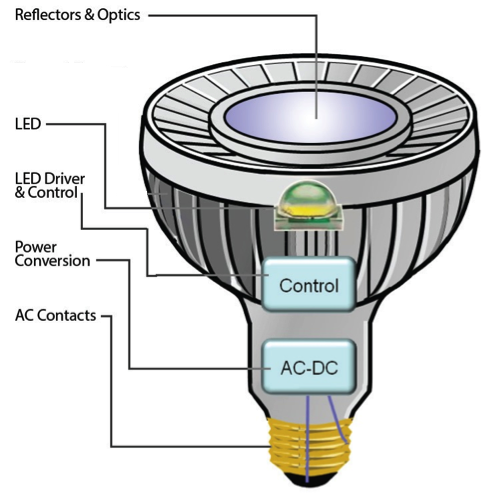
\includegraphics[width  = \textwidth]{otherlightbulb}
    \caption{\textbf{LED system \cite{Schweber}.}}
    \label{fig:led}
\end{minipage}\hfill
 \begin{minipage}[t]{0.42\textwidth}
    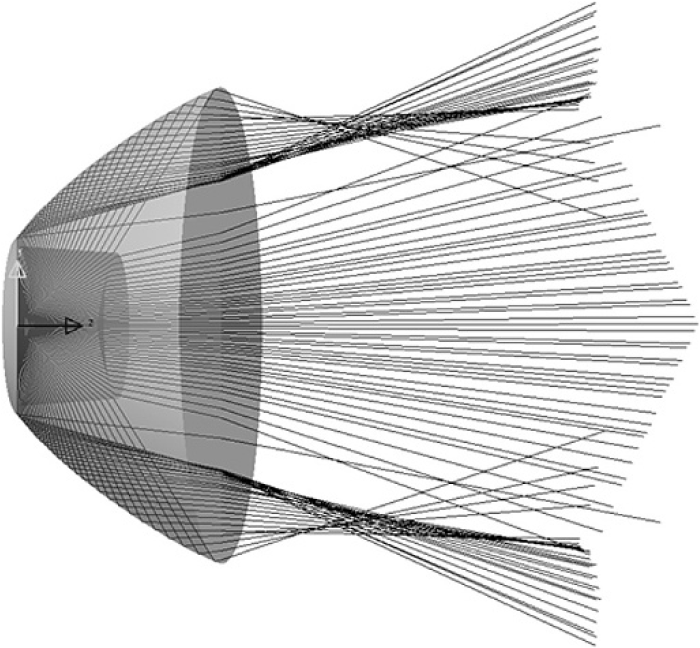
\includegraphics[width  = \textwidth]{TIR3D}
    \caption{\textbf{Example of an optical system.} A total internal reflector in $3$D \cite{prins2014inverse}.}
    \label{fig:tir_example_3D}
\end{minipage}
\end{figure}

Illumination optics is the branch of optics that deals with the design of optical systems. It concerns the transfer of light from source to target. The goal in illumination optics is to obtain the desired light distribution at the receiver after its propagation through an optical system. Depending on the required intensity distribution, an optical engineer can determine what type of optics is needed. To this purpose, it is important to understand how light propagates through a given optical system.

Light can be seen as the electromagnetic radiation perceived by the human eye \cite{schreuder2008outdoor}. Therefore, it propagates as an electromagnetic wave and, as such, it has a certain wavelength. Visible light has wavelength in the range between $400$ and $700$ nm. Usually the wavelength of light is extremely small compared to the dimensions of the optics with which it interacts, so it is reasonable to consider the limit of infinitely short wavelengths. The field of optics that discards the microscopic wave behavior of light is called \textit{geometric optics}. In the geometric optics approximation, light is described by rays that propagate perpendicularly to the wavefront, transporting electromagnetic energy. Since the dimensions of the optical components used for illumination systems are very big compared to the wavelength of visible light, illumination optics is usually described in terms of geometric optics \cite{born2013principles}. 

To compute photometric variables at the target of an
optical system, the ray tracing procedure is widely used in the field of geometric optics \cite{glassner1989introduction}.
Ray tracing is a forward method which provides the light distribution at the target given a light source and an optical system \cite{Gross2005Handbook}. Every ray is considered to be a straight line when propagating in free space. Once the ray hits an optical surface its direction changes according to reflection and refraction laws. Ray tracing computes the intersection points of every ray emitted from the source with \textit{all} the optical surfaces that it encounters. Next, it calculates the surface at the closest distance from the point where the ray was emitted. The new ray direction at the intersection point ray is computed. The procedure continues until the ray reaches the target. These steps are repeated for all the rays traced.
There are many ways to implement the ray tracing process.

Monte Carlo (MC) ray tracing is often used in non-imaging
optics. This method is based on a probabilistic interpretation
of the rays distribution at the source of the optical
system \cite{liu2010precise,Ting:1}: many rays are traced randomly from the source,
and their distribution at the target is estimated to compute the
photometric variables of the output light. For example, the output intensity distribution is provided dividing the target into equal cells and counting the number of rays that arrive at each cell of the target. Although the MC
procedure constitutes a robust method, it remains a slow and
numerically costly procedure, as it converges proportionally
to the reciprocal value of the square root of the number of rays
traced. Therefore, to obtain a good accuracy of the intensity distribution at the target, millions of rays need to be traced.

To speed up MC ray tracing, deterministic Quasi-Monte Carlo (QMC) ray tracing was introduced. The difference between MC and QMC is that in the latter the coordinates of the rays traced are distributed according to \textit{low-discrepancy sequences}. Intuitively, the discrepancy indicates how much the rays distribution differs from a uniform distribution.  Hence, low discrepancy sequences are close to uniformly distributed sequences \cite{levy2002introduction}.
Numerical simulations show that in most cases QMC ray tracing is an improvement of MC ray tracing \cite{ohbuchi1996quasi, caflisch1998monte}. However, it is not possible to predict the convergence of QMC ray tracing as the error is always bounded by a term proportional to the discrepancy of the initial sample of rays \cite{tuffin2004randomization}.

The purpose of this thesis is to provide tools to improve illumination optics design by using faster and more accurate methods than the current state-of-the-art ray tracing methods.
To do so, we analyze optical systems using the concept of \textit{phase space} (PS) \cite{torre2005linear}.
The PS of an optical surface is described by the position and direction coordinates of all the rays that hit the surface \cite{testorf2009phase}. We restrict ourselves to the two-dimensional case, which is particularly relevant as it constitutes a good test case to
demonstrate the performance of the new ray tracing method. For any rotationally symmetric
system, the 2D case is very useful to study. Optical designers often start working in two dimensions where only the
meridional plane is taken into account. In two dimensions we refer to \textit{optical lines} instead of optical surfaces. The PS of a two-dimensional system is a two-dimensional space described by all the possible ray positions and directions. 

Optical phenomena can be analyzed by using the PS, and photometric variables can be defined in PS as well \cite{rausch2014illumination}.  
%For example, the \'{e}tendue can be seen as the area covered by the rays in phase space which can be calculated either using numerical integration or, for very simple systems, even analytically. The luminance is the power distribution in phase space. For systems formed by a Lambertian source the output luminance is a positive constant when different from zero. The intensity is given by an integration of the luminance over all the possible positions in phase space. Assuming a Lambertian source, the intensity along every direction is simply the support of the luminance given by the sum of the distances between the rays located on the boundaries of the regions with positive luminance. 
Currently, some literature based on phase space optics has been published, showing that light propagation can be investigated using the PS concept \cite{rausch2012phase,rausch2014phase, herkommer2012phase}. 
In particular, it has been proved that the radiance and irradiance distribution at the target can be analyzed by looking at PS transformations from source to target.
Also, PS optics might constitute an alternative approach for describing aberration phenomena \cite{herkommer2013phase, babington2017freeform, wolf1993relativistic}. In this thesis we introduce new methods based on PS providing a new way to calculate the light distribution at the target of optical systems. Our PS methods allows tracing less rays inside the system than existing procedures, i.e., MC and QMC ray tracing. This significantly reduces the computational time compared to conventional ray tracing.
Next, the methods and results are briefly discussed. 
\section{Phase space methods and results}
The new methods presented in this thesis are based on PS rays tracing. The PS of a line is a $2$D space defined by all possible position and one-direction coordinate of rays that hit the line. 
The position coordinate is given by one of the two coordinates of the intersection point between the rays and the optical line. The direction coordinate is the sine of the angle $t$ that the ray forms with the normal of the line encountered, measured counterclockwise and multiplied by the index of refraction $n$ of the material in which the line is located \cite{wolf2004geometric}. In Figure \ref{fig:TIR_intro} we show a ray propagating inside a two-dimensional optical system in the $(\variabile{x}, \variabile{z})$-plane. This ray is described by a unique point in target PS with corresponding coordinates $(\variabile{x}, n\sin(t))$ (see Figure \ref{fig:PS_intro}).
\begin{figure}[t]
  \begin{minipage}[t]{0.49\textwidth}
    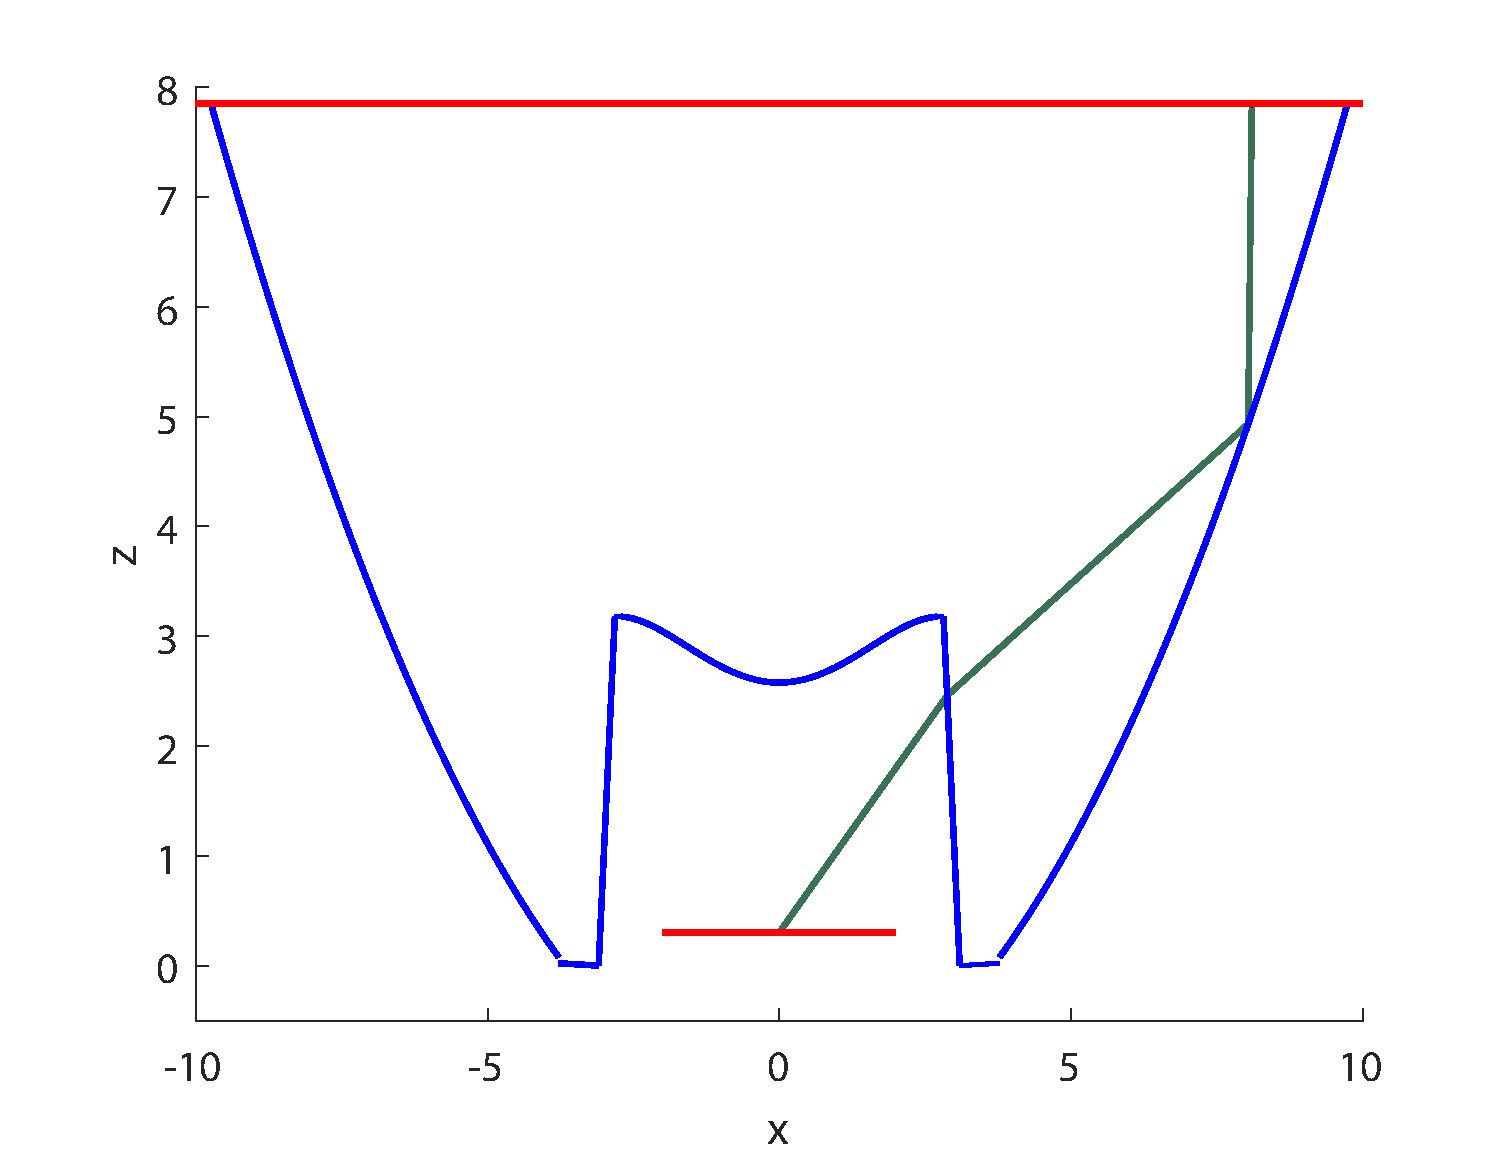
\includegraphics[width  = \textwidth]{tir_1ray}
    \caption{\textbf{A ray propagating inside an optical system.}}
    \label{fig:TIR_intro}
  \end{minipage}
\hfill
  \begin{minipage}[t]{0.47\textwidth}
    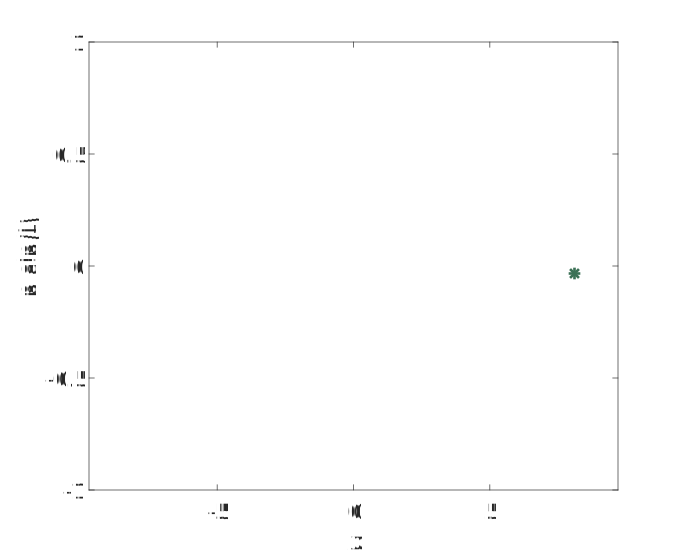
\includegraphics[width=\textwidth]{PS_tir_1ray}
  \caption{\textbf{Ray at the target PS of the system.} A ray in PS is a point with coordinates $(x, n\sin(t))$.}
\label{fig:PS_intro}
 \end{minipage}
\end{figure}
PS ray tracing takes into account the \textit{path} followed by every ray, that is, the sequence of the optical components encountered by every ray traced.
Considering, for every ray traced, its corresponding path, we observe that the PS of the source and the target are partitioned into regions, each of them corresponds to rays that follow the same path. 
While the source PS is completely covered by these rays, the target PS is not.

The boundaries of the regions in target PS give important information about the output photometric variables because there the target luminance has a jump discontinuity from zero to a positive value. 
%LED light sources are close to Lambertian, i.e., they emit equal luminance in every direction \cite{taylor2000illumination}. For systems with a Lambertian source the boundaries of these regions give \textit{all} the information needed for computing the luminance and the intensity and, as a consequence, it is not required to trace rays that will be located in the interior of these regions.
%In the general case of a non-Lambertian source, a sample of rays inside 
The positive luminance regions should be considered over all the possible directions to provide the profile of the output luminance, and numerical integration gives the target intensity profile. Detecting the boundaries of the positive luminance regions, the photometric variables can be quickly computed without the need for tracing millions of rays, which is instead necessary for conventional procedures such as MC and QMC ray tracing. We focus on two different procedures: phase space ray tracing and backward ray mapping in phase space.

\textit{Phase space ray tracing} is a forward method that employs the source and the target PS representation of the optical system. The key idea is to construct a nonuniform triangulation in source PS such that more triangles are defined close to the discontinuity of the luminance. The coordinates of the vertices of each triangle correspond to the coordinates of the rays traced that will be located close to the discontinuities of the luminance. In order to compute the target photometric variables, the boundaries of the positive luminance regions need to be calculated. 
%Assuming a Lambertian source, these boundaries give \textit{all} the information needed for the luminance and the intensity calculation. 
Therefore, we provide two different approaches to obtain an approximation of the boundaries at the source PS.

The first technique is based on $\alpha$-shapes. 
Given a triangulation in source PS (usually the Delanauy triangulation \cite{marsden2003texts}), a parameter $\alpha$ is used to decide which triangles have to be included for the boundaries computation and which have to be removed. In general it is not easy to establish the value of $\alpha$ that gives the desired boundary computation \cite{teichmann1998surface}. We develop a procedure based on \'{e}tendue conservation \cite{filosa2015new}. 

The second technique for the boundaries computation exploits the triangulation refinement explained above. The approximation of the boundaries in source PS is obtained by connecting the vertices on one side of the boundary between two regions, corresponding to rays that follow different paths.
%The $\alpha$-shapes method considers a triangulation (usually the Delanauy triangulation \cite{marsden2003texts}) of the set of points obtained from the triangulation refinement of the source PS. Then, the parameter $\alpha$ is used to decide which triangles have to be considered for the boundaries computation and which have to be removed. For every triangle the radius of its circumcircle is considered. If it is greater than $\alpha$, then the triangle is eliminated from the triangulation. Connecting the edges of the remaining triangles belonging to only one triangle, the $\alpha$-shape of the points cloud is found. In general it is not easy to establish the value of parameter $\alpha$ that gives the desired boundary computation \cite{teichmann1998surface}. We develop a procedure based on \'{e}tendue conservation \cite{filosa2015new}. \\ \indent The second technique for the boundaries computation exploits the triangulation refinement explained above. The approximation of the boundaries in source PS is obtained by connecting the vertices on one side of the boundary between two regions, corresponding to rays that follow different paths. The finer the triangulation, the more accurate the boundaries are. 
\'{E}tendue conservation is used to provide a stopping criterion for the triangulation refinement \cite{filosa2016ray, filosa2017phase}.  

Once the boundaries are calculated at the source PS, also the boundaries at the target are obtained (edge-ray principle, \cite{Ries:2}). Assuming a Lambertian source, the output intensity is calculated by only tracing the rays located on these boundaries. 

Numerical results are provided using both $\alpha$-shapes and the triangulation refinement for several optical systems.
To validate the method, the intensities found are compared to both MC and QMC simulations. The results demonstrate that using PS ray tracing allows tracing far less rays than MC ray tracing to obtain an accurate approximation of the intensity profile. However, when using $\alpha$-shapes, the number of rays traced depends on the complexity of the design of the optical system. On the other hand, computing the boundaries employing the triangulation refinement, a speed of convergence proportional to the inverse of the number of rays traced is obtained for all the systems considered versus a speed of convergence proportional to the inverse of the square root of the number of rays traced for MC ray tracing. Numerical simulations show that PS ray tracing based on the triangulation refinement gives speed advantages also comparable with QMC ray tracing when applied to some optical systems, while it is slower than QMC for some other systems.
PS ray tracing is therefore further improved by introducing the backward ray mapping method based on a ray mapping reconstruction in PS. 

\textit{Backward ray mapping in phase space} is first developed for systems formed by straight line segments. In this case, the phase spaces of \textit{all} the lines that constitute the system are considered. We assume that the optical lines are designed such that they can both receive and emit light while the source can only emit light and the target only receive it. Both source and target PS of each line are computed, and only one PS is implemented for the source and the target. Concatenating all the PSs with two different maps, we are able to construct an inverse map from the target to the source. This explains the name \textit{concatenated backward ray mapping} for this method. Numerical results show that only the rays on the target PS located \textit{exactly} at the boundaries of the positive luminance regions are traced. The output intensity is computed by integrating the luminance at the target PS. A comparison between concatenated backward ray mapping and QMC ray tracing demonstrates that our method computes the \textit{exact} intensity, significantly reducing the computational time. 

In order to modify the method to systems including curved lines, we use a different approach, which employs the PS representation of only the target of the optical system. Applying a bisection method combined with backward ray tracing, we are able to construct the inverse map from the target to the source \textit{directly}. This allows tracing only the rays at the boundaries of the positive luminance regions \cite{filosa2017inverse}. From these rays the output intensity is calculated. We show in simulations that \textit{direct backward ray mapping} is more accurate and faster than QMC ray tracing.

Finally, direct backward ray mapping is modified for systems with Fresnel reflections. In this case every ray incident on a Fresnel lens is split into a reflected and a refracted ray, each of them carry a fraction of the energy of the incident ray. This leads to a multitude of possible paths. 
%Direct backward ray mapping is applied considering every possible path separately. Given a path the rays located on the boundary of the corresponding region in target PS are traced from the target to the source. 
Numerical simulations show that direct backward ray mapping is able to detect \textit{all} the possible paths and to determine the boundaries of \textit{all} the positive luminance regions in target PS. Since, for Fresnel systems, the luminance is not constant at the target, a sample of rays inside those regions needs to be traced for calculating the luminance and the intensity profile.
\section{Outline of this thesis}
This work is organized in the following way.

In Chapter \ref{chap:Illumination optics} an overview of the physics of illumination optics is provided. After a short introduction of radiometric variables, the photometric counterparts are defined. The reflection and refraction laws are described and total internal reflection is discussed. A description of Fresnel reflection is included. In this chapter we follow the literature reported in \cite{hecht1998hecht, feynman2011feynman, feynman1964feynman}.

Chapter \ref{chap:raytracing} includes a discussion on classical ray tracing. In particular, MC and QMC ray tracing are discussed. They are based on a combination of MC and QMC procedures with ray tracing methods. We explain how to calculate the target intensity using these techniques. Numerical results for a simple system show the convergence of the approximated intensities to the exact intensity by increasing the number of rays traced.

Chapter \ref{chap:PS} introduces the PS concept for two-dimensional optical systems. We show that the PS provides a complete description of optical systems. We explain how to construct the triangulation refinement on which PS ray tracing is based. The PS representation of both source and target of a simple system (the two-faceted cup) shows that the phase spaces are divided into several regions formed by rays that follow the same path when they propagates through the system. Two techniques for calculating the boundaries of these regions are provided next. 
 
A method based on $\alpha$-shapes is presented in Chapter \ref{chap:boundaries_alpha}. A technique based on \'{e}tendue conservation is developed and numerical results for two different total internal reflection (TIR)-collimators are provided. For these systems also the target intensity in PS is calculated and it is compared with MC ray tracing. The chapter ends with a discussion of the results obtained.

A different approach for the boundaries calculation, which employs a triangulation refinement in source PS, is presented in Chapter \ref{chap:triangulation}. The method is applied to three different systems: the two-faceted cup, a TIR-collimator and a parabolic reflector. Numerical results are compared with both MC and QMC ray tracing.

Next, a second method based on ray mapping reconstruction from the target to the source is developed. Chapter \ref{chap:raymapping1} includes the description of concatenated backward ray mapping for systems formed by straight and reflective line segments. The target intensity is computed for two different optical systems: the two-faceted cup and a multifaceted cup. Numerical results are compared to QMC ray tracing. 

In Chapter \ref{chap:raymapping2} we present the direct backward ray mapping method, which is a modification to systems including curved and refractive lines. A detailed explanation of the idea and the algorithm used are given. The results for the TIR-collimator and the parabolic reflector validate the method showing that it calculates the intensity correctly. 

The research is concluded with Chapter \ref{chap:fresnel}, which discusses direct backward ray mapping applied to systems with Fresnel reflection. The theoretical explanation of the method is followed by numerical results applied to a system formed by the source, the target and a simple convex lens. We show in simulations that the boundaries of the positive luminance regions are calculated correctly. Finally, the profile of the luminance is obtained considering a sample of rays inside these regions and the intensity is given by integrating the luminance over all the possible positions. 

Chapter \ref{chap:conclusions} summaries the finding and presents discussions and insights for future research.

Two appendices provide technical details about MC integration and MC ray tracing, and the exact computation of the target intensity for the two-faceted cup.
\clearpage{\pagestyle{empty}\cleardoublepage}
 
\chapter{Illumination optics}\label{chap:Illumination optics}
% Explain what is a ra
This chapter provides some concepts of illumination optics used in this thesis. We start explaining the difference between radiometry and photometry.
In particular, we focus on the photometric variables, defining them both in three and two dimensions. The reflection and refraction laws and the phenomenon of total internal reflection are explained next. The last paragraph of the chapter gives a brief introduction to Fresnel reflection. 
\section{Radiometric and photometric variables}\label{sec:photometry}
Radiometry is concerned with the measurement of electromagnetic radiation across the entire electromagnetic spectrum. Photometry is the subfield of radiometry that takes into account only the portion of the electromagnetic spectrum corresponding to the visible light \cite{zalewski1995radiometry}. Radiometry deals with radiometric quantities. An important radiometric quantity  is the radiant flux $\Phi_{\textrm{r}}$ (unit watt \textrm{W}) which is the total energy emitted from a source or received by a target per unit time:
\begin{equation}
\Phi_{\textrm{r}} = \frac{\textrm{d}Q}{\textrm{d}\mytime}\,,
\end{equation}
where $Q$ is the energy and $\mytime$ the time.\\
\indent In illumination optics the measurement of light is given in terms of the impression that it gives on the human eye. Therefore, illumination optics deals with photometric variables rather than with radiometric variables. The most important photometric variables are defined in the following using the notation adopted by Chaves in \cite{chaves2015introduction}. The luminous flux $\Phi$ (unit lumen \textrm{lm}) is defined as the \textit{perceived} power of light by the human eye.
 The radiant and the luminous flux are related by the luminous efficacy function $y$, unit \textrm{lm}/\textrm{W}, which defines how many lumen correspond to one Watt of power at a given wavelength.
 The luminous efficacy function reaches its maximum  at a wavelength of $555$ $\textrm{nm}$ where it is equal to $683$ $\textrm{lm}/\textrm{W}$.
  We may normalize the luminous efficacy function with its maximum value of $683$.
  The normalized function $\bar{y}(\lambda)$ is the luminous efficiency shown in Figure $\ref{fig:luminosityfunction}$ where $\lambda$ is the wavelength. It is a \textit{dimensionless} quantity with a range of value between $0$ and $1$ \cite{schubert2005light}.
\begin{figure}[h]
%\label{fig:luminousfunction}  
  \begin{center}
  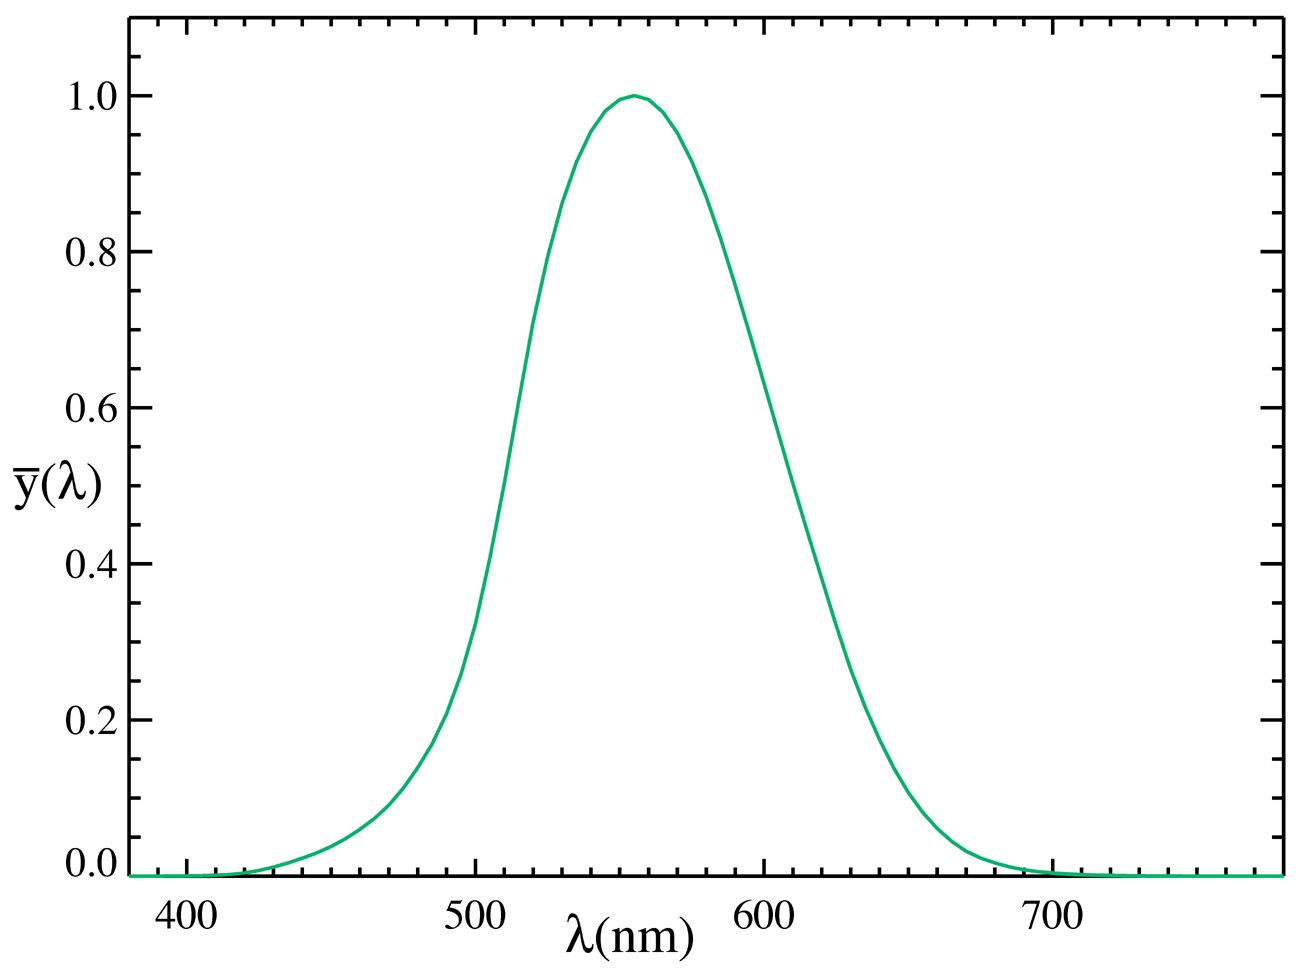
\includegraphics[width=7cm]{CIELuminosity}
  \end{center}
  \caption{\textbf{Luminosity function $\bar{y}(\lambda)$}. relation between the eye's sensitivity and the wavelength of light. The luminosity function is dimensionless  \cite{wiki}.}
  \label{fig:luminosityfunction}
  \end{figure}
\\ \indent The luminous flux corresponding to one Watt of radiation power at any wavelength is given by the product of $683$ $\textrm{lm/W}$ and the luminosity function at the same wavelength,
i.e. $683 \, \bar{y}(\lambda)$. Hence, the total luminous flux $\Phi$ has unit lumen (\textrm{lm}) and it is defined as:
\begin{equation}\label{eq:luminous_flux}
\Phi = 683 \int_0^\infty \Psi_\textrm{r}(\lambda) \bar{y}(\lambda)\textrm{d}\lambda,
\end{equation}
where $\Psi_\textrm{r}(\lambda)$ is the spectral radiant flux, i.e. the power (in Watt) per unit wavelength (unit \textrm{W}/\textrm{m}). The corresponding photometric variable of is the spectral luminous flux $\Psi(\lambda)$ (unit \textrm{lm}/\textrm{m}), i.e. the flux as perceived by the human eye as a function of the wavelength. 
Using the relation following between $\Psi_\textrm{r}$ and $\Psi$:
\begin{equation}
683 \bar{y} = \frac{\Psi}{\Psi}, 
\end{equation}
Equation (\ref{eq:luminous_flux}) can be written as:
\begin{equation}
\Phi = \int_0^\infty \Psi(\lambda)\textrm{d}\lambda.
\end{equation}
%% Explain while integrals between 0 and infinity
%The luminous emittance $M = M(\vect{x}, \myangle)$ is the total flux emitted in all direction from a unit area. It is measured in lumens pr square meters (\textrm{lm}/$\textrm{m}^2$).
\\ \indent Geometric optics describes a beam of light as a collection of parallel light rays, where a light ray can be interpreted as a line or curve along which the energy travels. A ray is always direct perpendicular to the light's wavefront.  
The infinitesimal luminous flux $\textrm{d}\Phi$ incident on an infinitesimal surface $\textrm{d}A$ is called illuminance $E$ (unit $\textrm{lm}/\textrm{m}^2$)
and is defined as:
\begin{equation}
 E=E(\vect{x}) = \frac{\textrm{d}\Phi}{\textrm{d}A}\;,
 \end{equation}
The corresponding radiometric variable is called \textit{irradiance}, we indicate it with $P$. The density of light emitted by a point source in a given direction is determined by the solid angle.\\ \indent
The solid angle in a given direction is expressed by a cone of rays emitted in that particular direction by a point source located at the center of the unit sphere \cite{koshel2012illumination}. 
Let $\textrm{d}S$ be the area on the unit sphere subtended by the cone,
the infinitesimal solid angle $\textrm{d}\Omega$ is given by:
\begin{equation}\label{solid_angle}
\textrm{d}\Omega = \textrm{d}S= \sin(\theta)\textrm{d}\theta \textrm{d}\phi\,
\end{equation}
 where $\myangle$ and $\phi$ are the polar and the azimuthal angle that the normal $\boldsymbol{\nu}$ to the infinitesimal area $\textrm{d}A$ makes with the direction of the central line of $\textrm{d}\Omega$, respectively (see Figure \ref{fig:rad}).
The solid angle on the entire unit sphere is $\Omega = 4\pi$ and its unit is steradian $\textrm{sr}$ \cite{arecchi2007field}.
The luminous intensity $I$ (unit candela $\textrm{cd}=\textrm{lm}/\textrm{sr}$) is defined as the luminous flux $\textrm{d}\Phi$ per solid angle
$\textrm{d}\Omega$ and is given by:
\begin{equation}\label{intensity}
I = I(\myangle, \phi) = \frac{\textrm{d}\Phi}{\textrm{d}\Omega}\;.
\end{equation}
 \begin{figure}[h]
%\label{fig:cup}
  \begin{center}
  \includegraphics[width=6 cm]{SolidAngle}
  \end{center}
  \caption{\textbf{Solid angle}. $\textrm{d}\Omega$ is in a given direction $\myangle$ with $\myangle$ the angle that the central line forms with the normal to the area $\textrm{d}A$.}
  \label{fig:rad}
  \end{figure}
\\ \indent Let us now consider a finite source $\textrm{d}A$.
The luminance $L = L(\vect{x}, \myangle)$ (unit $\textrm{cd} / \textrm{m}^2$) depends both on the position and the direction, it is the luminous flux per unit solid angle $\textrm{d}\Omega$ and  per unit projected area $\cos\myangle \textrm{d}A$.  $L$  is given by:
\begin{equation}\label{luminance1}
  L=L(\vect{x}, \myangle) = \frac{\textrm{d}\Phi}{\cos\myangle\textrm{d}A\textrm{d}\Omega}\,.
\end{equation}
\noindent Note that from ($\ref{intensity}$) and ($\ref{luminance1}$) we can derive a relation between the intensity and the luminance. 
The intensity $I$ emitted by the infinitesimal area $\textrm{d}A$ is given by:
\begin{equation}\label{eq:int_lum}
I = \frac{\textrm{d}\Phi}{\textrm{d}\Omega}= L(\vect{x},\myangle)\cos\myangle\textrm{d}A \,.
\end{equation}
When the luminance is uniform over a finite area $A$, the luminous intensity emitted in the direction $\myangle$ is:
\begin{equation}
I(\vect{x}, \myangle) = I(\myangle) = L(\myangle) A \cos\myangle\,.
\end{equation}
Thus, when $L(\vect{x},\myangle)$ does not depend on the position and the direction (i.e. $L(\vect{x},\myangle)=L$), we obtain Lambert's cosine law:
\begin{equation}
I(\myangle) = I_0\cos\myangle ,
\end{equation}
where $I_0 = I(\myangle = 0) = LA$. Light sources emitting light with a constant luminance are called \textit{Lambertian} sources.\\
\indent Finally, we give a definition of the \'{e}tendue $U$ (unit $\textrm{m}^2\textrm{sr}$).
Etendue is a french word that means extent or spread. In geometric optics, it is a quantity to describe how light is spread out in terms of area and solid angle \cite{lerner2006etendue, zhu2011etendue}.
The quantity $ \textrm{d}U $ of a source $\textrm{d}A$ is defined as:
\begin{equation}\label{etendue}
\textrm{d}U = n^2  \frac{1}{L}\textrm{d}\Phi = n^2 \cos\myangle\textrm{d}A\textrm{d}\Omega,
\end{equation}
where $n$ is the index of refraction of the medium in which $\textrm{d}A$ is immersed. In phase space optics the \'{e}tendue is considered to be a volume in phase space (or an area for two-dimensional systems). This concept will be clarified in Chapter \ref{chap:PS} in which we treat the phase space in more detail.
An important \'{e}tendue property is its conservation within an optical system in absence of absorption. 
In the following we show, using the approach of Chaves in \cite{chaves2015introduction}, 
how conserservation of \'{e}tendue in a lossless system can be derived. For the optical systems we will consider in this work, the source and the target are located in the same medium (air) with $n=1$, so the luminance $L$ equals the basic luminance $L^* = L/n^2$ at the source and the target of the system. 
Consider a light ray emitted from an infinitesimal area $\textrm{d}A_1$ to the area $\textrm{d}A_2$. Suppose that the centers of $\textrm{d}A_1$ and $\textrm{d}A_2$ 
are located at a distance \variabile{d} from each other, see Figure \ref{fig:etendue_conservation}.
\begin{figure}[t]
 \label{fig:etendue_conservation}
     \begin{center}
     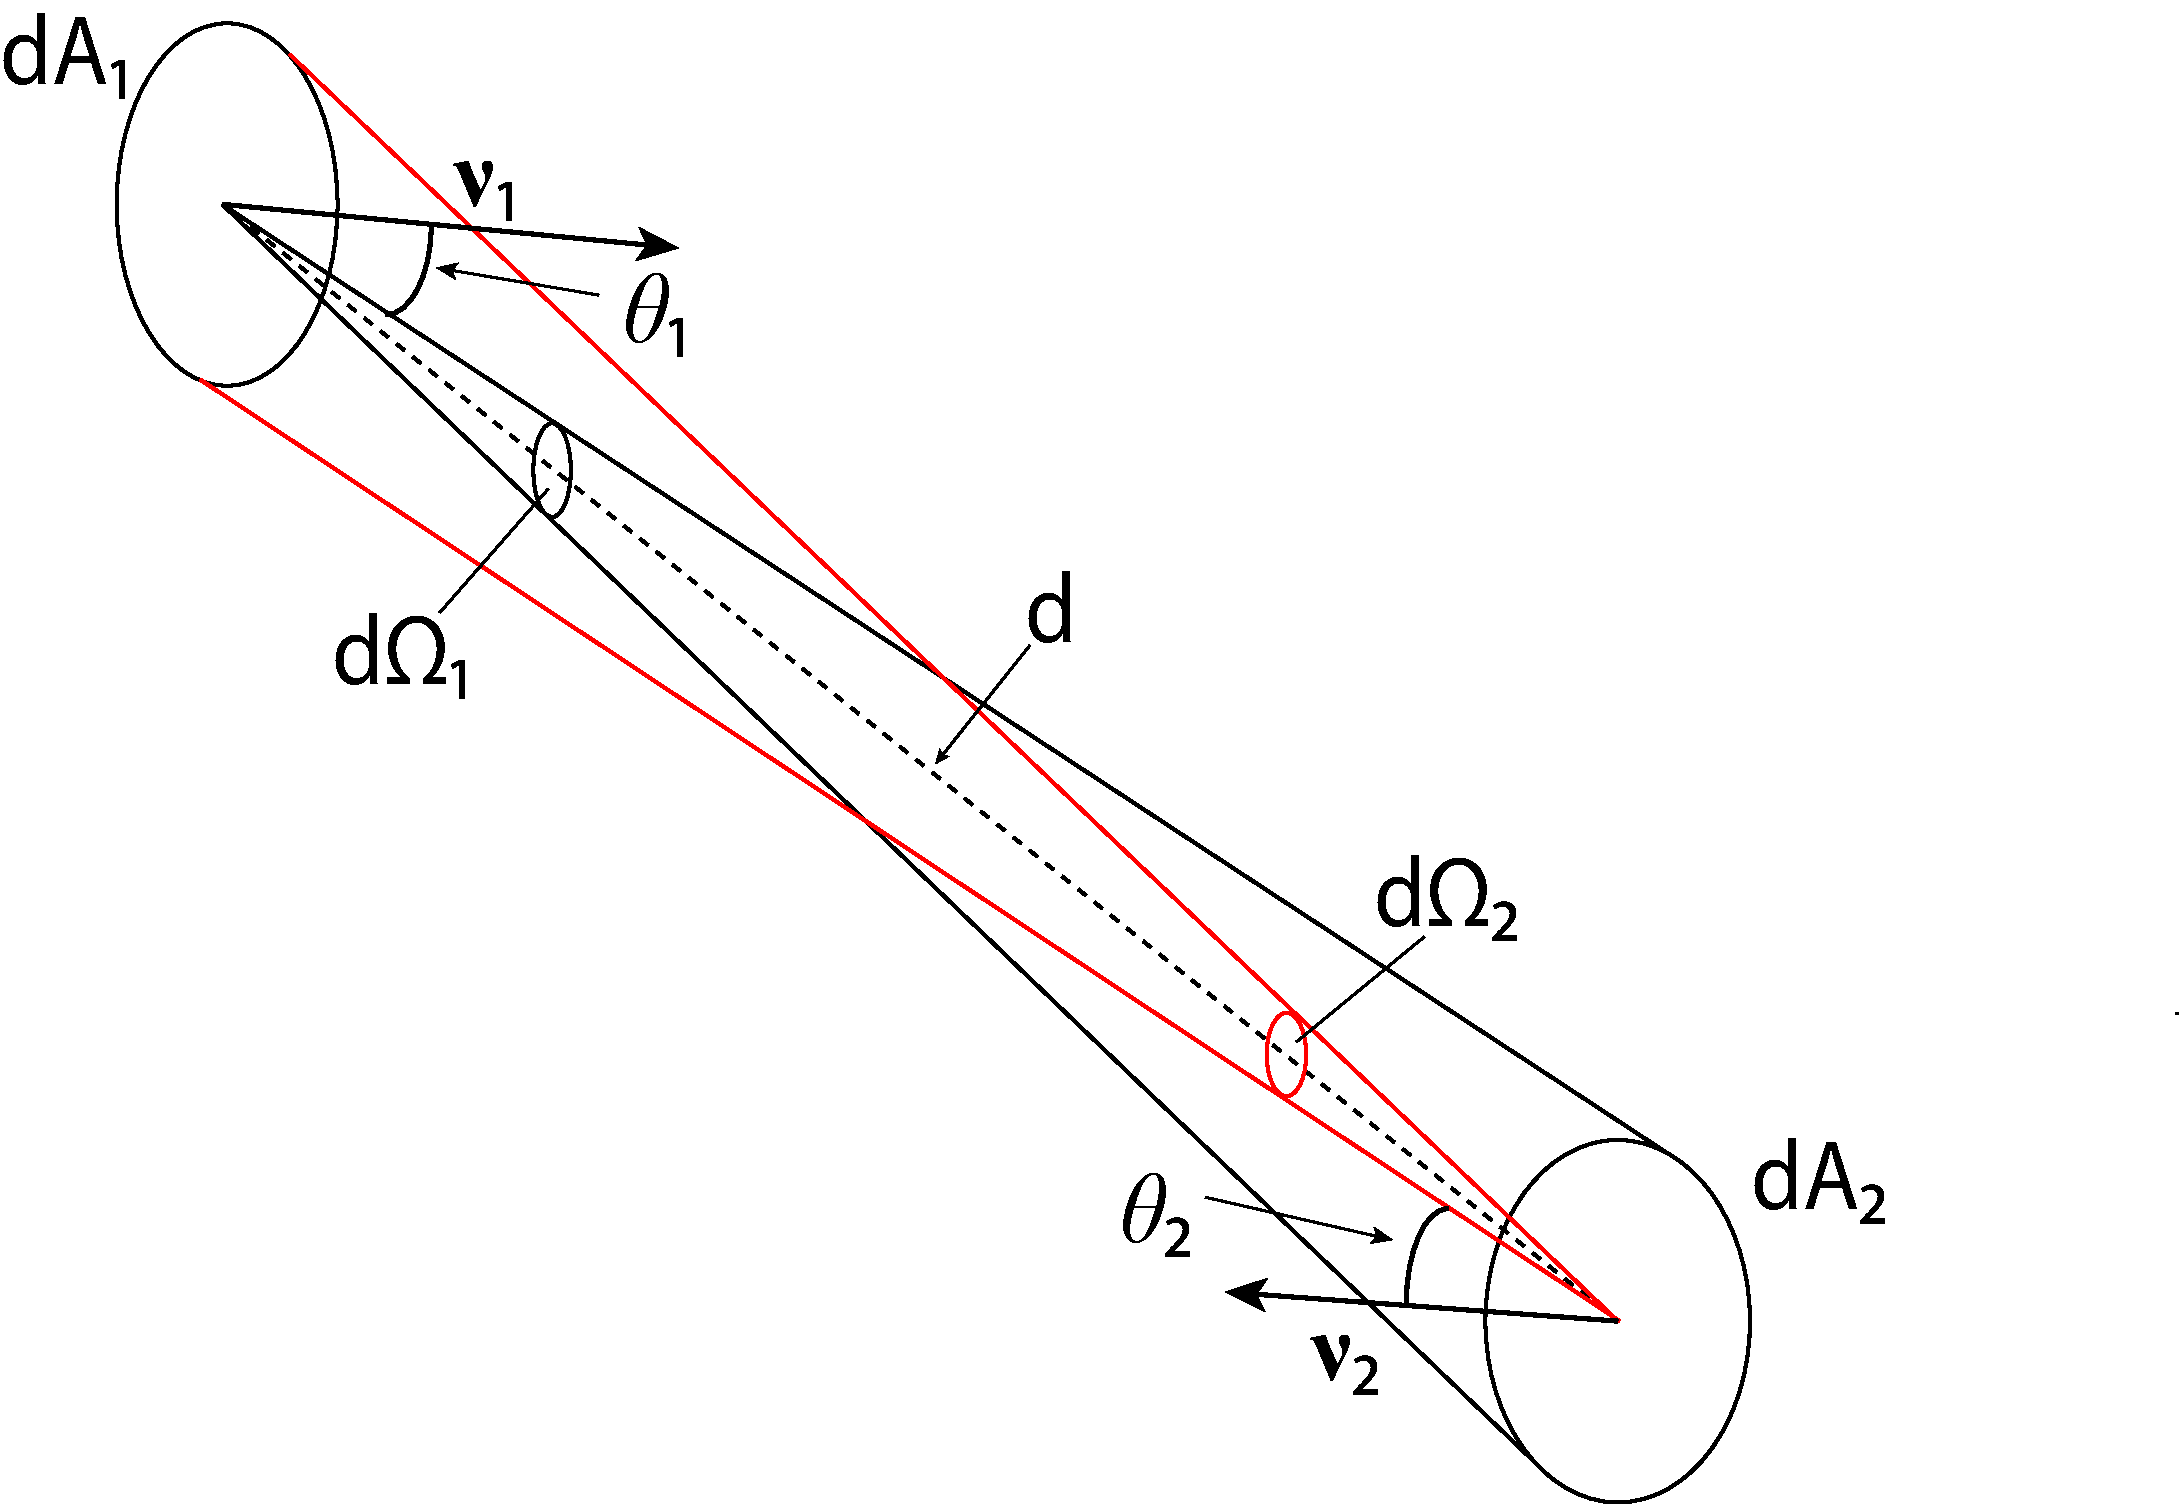
\includegraphics[width=10cm]{areas.pdf}
     \end{center}
     \caption{\textbf{Transfer of flux from the source $\textrm{d}A_1$ to the target $\textrm{d}A_2$.} $\textrm{d}A_1$ and $\textrm{d}A_2$ are two surfaces with normals $\nu_1$ and $\nu_2$, respectively. Their centers are located at a distance \variabile{d}.
$\myangle_1$ and $\myangle_2$ are the angles made by the central ray with the normals $\nu_1$ and $\nu_2$, respectively.}
\label{fig:etendue_conservation}
 \end{figure}
We derive \'{e}tendue conservation for the case in which $\textrm{d}A_1$ and $\textrm{d}A_2$ are located in the same medium (see \cite{chaves2015introduction, koshel2012illumination} for the general case).
We indicate with $\boldsymbol{\nu}_1$ and $\boldsymbol{\nu}_2$ the normals to the surfaces $\textrm{d}A_1$ and $\textrm{d}A_2$, and with $\myangle_1$ and $\myangle_2$ the angles that the ray connecting the centers of $\textrm{d}A_1$ and $\textrm{d}A_2$ forms with $\boldsymbol{\nu}_1$ and $\boldsymbol{\nu}_2$. The differential solid angle $\textrm{d}\Omega_1$ subtended by $\textrm{d}A_2$ at the center of $\textrm{d}A_1$ and the flux $\textrm{d}\Phi_1$ passing through $\textrm{d}A_2$ emitted from $\textrm{d}A_1$ and the corresponding solid angle are defined as:
\begin{subequations}
\begin{align}
\label{eq:omega1}
\textrm{d}\Omega_1 &= \frac{\textrm{d}A_2\cos(\myangle_2)}{\variabile{d}^2}\,,\\
\textrm{d}\Phi_1 &= L_1 \cos\myangle_1 \textrm{d}A_1 \textrm{d}\Omega_1. \label{eq:phi1}
\end{align}
\end{subequations}
Similarly, the differential solid angle $\textrm{d}\Omega_2$ subtended by $\textrm{d}A_1$ at the center of $\textrm{d}A_2$ and the flux $\textrm{d}\Phi_2$ passing through $\textrm{d}A_1$ emitted from $\textrm{d}A_2$ are equal to:
\begin{subequations}\begin{align}\label{eq:omega2}
\textrm{d}\Omega_2 &= \frac{\textrm{d}A_1\cos\myangle_1}{\variabile{d}^2}\,,\\
\textrm{d}\Phi_2 &= L_2 \cos\myangle_2 \textrm{d}A_2 \textrm{d}\Omega_2.\label{eq:phi2}
\end{align}
\end{subequations}
Then from Equation (\ref{etendue}) we obtain the following relations: 
\begin{subequations}
\begin{align}
\textrm{d}U_1 &= n^2\cos\myangle_1 \textrm{d}A_1\textrm{d}\Omega_1= \frac{n^2\cos\myangle_1 \textrm{d}A_1\textrm{d}A_2\cos\myangle_2}{\variabile{d}^2},\\
\textrm{d}U_2 &= n^2 \cos\myangle_2\textrm{d}A_2\textrm{d}\Omega_2= \frac{ n^2 \cos\myangle_2\textrm{d}A_2\textrm{d}A_1\cos\myangle_1}{\variabile{d}^2}, \label{eq:dU2}
%\end{split}
\end{align}
\end{subequations}
for $\textrm{d}A_1$ and $\textrm{d}A_2$, respectively.
%From equation ($\ref{etendue1}$) and ($\ref{etendue2}$) 
From the previous equations we can conclude that $\textrm{d}U_1=\textrm{d}U_2$ and therefore the \'{e}tendue is conserved along a beam of light. 
Since the system is a lossless system energy is conserved from the source to the target ($\textrm{d}\Phi_1= \textrm{d}\Phi_2$), therefore the \'{e}tendue conservation implies:
\begin{equation}\label{basicluminance}
L_1 = n^2 \frac{\textrm{d}\Phi_1}{\textrm{d}U_1} = n^2 \frac{\textrm{d}\Phi_2}{\textrm{d}U_2} = L_2\,,
\end{equation}
where the first equality comes from Equation (\ref{luminance1}) combined with Equation (\ref{etendue}).
In this thesis we consider two-dimensional optical systems. 
 Hence, the definitions of the photometric parameters have to be adapted in two-dimensions. An infinitesimal line segment of length $\textrm{d}\variabile{a}$ emitting a ray that makes an angle $\myangle$ with the normal $\boldsymbol{\nu}$ are considered, see Figure \ref{fig:2Dsolidangle}. 
\begin{figure}[t]
 \label{fig:2Dsolidangle}
     \begin{center}
     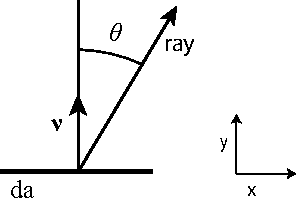
\includegraphics[width=7cm]{solidangle2D.pdf}
     \end{center}
     \caption{\textbf{Ray emitted by an infinitesimal line segment.} $\textrm{d}a$ makes an angle $\myangle$ with respect to the line normal $\boldsymbol{\nu}$.}
\label{fig:2Dsolidangle}
 \end{figure}
The two-dimensional illuminance (unit $\textrm{lm}/\textrm{m}$) denotes the luminous flux received by an infinitesimal line segment of length $\textrm{d}\variabile{a}$ 
and it is given by:
 \begin{equation}
 E=\frac{\textrm{d}\Phi}{\textrm{d}\variabile{a}}\;.
 \end{equation}
%The luminous emittance $M = M(\variabile{x}, \myangle)$ is the total flux emitted in all direction from a line segment.
The luminous intensity \big(unit $\big[\textrm{lm}/\textrm{rad}\big]$\big) is the luminous flux per angle $\textrm{d}\myangle$:
 \begin{equation}
 I=\frac{\textrm{d}\Phi}{\textrm{d}\myangle}\;.
 \end{equation}
 The two-dimensional luminance (unit $\textrm{lm}/(\textrm{rad}\,\textrm{m})$) is given by:
 \begin{equation}
 L= \frac{\textrm {d}\Phi}{\cos\myangle\,\textrm{d}\variabile{a} \,\textrm{d}\myangle}.
 \end{equation}
 Thus the following relation holds:
 \begin{equation}
 I = L(x, \myangle)\cos\myangle\,\textrm{d}\variabile{a}
 \end{equation}
where $x$ is a certain position at the light source $\textrm{d}\variabile{a}$. 
 Finally, the \'{e}tendue $\textrm{d}U $ (unit $\textrm{m}\;\textrm{rad}$) in two-dimensions is given by:
\begin{equation}\label{etendue2d}
\textrm{d}U = n\cos\myangle\textrm{d}\variabile{a}\,\textrm{d}\myangle.
\end{equation}
An overview of the photometric variables used in this thesis is given in Table \ref{tab:photometric_variables}
\begin{table}[t] 
\centering
\caption{\bf Photometric variables}
\begin{tabular}{lllll}
 \hline   \\
Name  & Symbol & Unit ($3D$) & Unit ($2D$) \\
  \hline 
Luminous flux & $\Phi$   & $\textrm{lm}$   &  $\textrm{lm}$ \\
%Spectral luminous flux & $\Phi_\lambda$   & $$   &  $1.75\cdot10^{-4}$ \\
Illuminance/emittance  & $E$    & $\textrm{lm}/{\textrm{m}^2} $ & $\textrm{lm}/{\textrm{m}^2}$  \\
Intensity  & $I$    & $\textrm{lm}/{\textrm{srad}} = \textrm{cd}$  & $\textrm{lm}/\textrm{rad}$ \\
Luminance  & $L$  & $ \textrm{cd}/{\textrm{m}^2}$   & $\textrm{lm}/(\textrm{rad} \,\textrm{m})$ \\
Etendue & $U$  & $\textrm{m}^2\; \textrm{srad}$   & $\textrm{m}\; \textrm{rad}$ \\
 \hline
 \end{tabular}
\label{tab:photometric_variables}
 \end{table}
\\ \indent In order to determine the light distribution on a surface and to compute the photometric variables on that surface, we need to understand how the light emitted from the source propagates. In the field of geometric optics the light propagation is described by light rays.
The propagation of a light ray traveling through  different media is determined by the reflection and refraction law.
In the following we introduce these two laws and we explain the total internal reflection phenomenon.
\section{Reflection and refraction law}\label{sec:reflection}
A light ray is described by a position vector \vect{x} on a surface and a direction vector \vect{t} and can be parameterized by the arc length \variabile{s}.
Light rays travel in a homogeneous medium along straight lines, once they hit a reflective surface their direction changes.
 Denoting with $\vect{t}_\textrm{i}$ the direction of the incident ray and with $\boldsymbol{\nu}$ the unit normal to the surface at the location of incidence, the direction $\vect{t}_\textrm{r}$ of the reflected ray is given by:
 \begin{equation}\label{Reflection}
  \vect{t}_\textrm{r} = \vect{t}_\textrm{i}-2 (\vect{t}_\textrm{i}\boldsymbol{\cdot}\boldsymbol{\nu})\boldsymbol{\nu},
\end{equation}
where the vectors $\vect{t}_\textrm{i}$ and $\boldsymbol{\nu}$ are unit vectors and $\vect{t}_\textrm{i}\boldsymbol{\cdot}\boldsymbol{\nu}$ indicates the scalar product of
$\vect{t}_\textrm{i}$ and $\boldsymbol{\nu}$. 
From the previous equation follows that the vector  $\vect{t}_\textrm{r}$ is a unit vector too, indeed considering the scalar product $\vect{t}_\textrm{r}\boldsymbol{\cdot}\vect{t}_\textrm{r}$ we conclude:
\begin{equation}\label{unit_vector}
\vect{t}_\textrm{r}\boldsymbol{\cdot}\vect{t}_\textrm{r} = \vect{t}_\textrm{i}\boldsymbol{\cdot}\vect{t}_\textrm{i} 
- 4(\vect{t}_\textrm{i}\boldsymbol{\cdot}\boldsymbol{\nu})(\vect{t}_\textrm{i}\boldsymbol{\cdot}\boldsymbol{\nu})+
4(\vect{t}_\textrm{i}\boldsymbol{\cdot}\boldsymbol{\nu})^2(\boldsymbol{\nu}\boldsymbol{\cdot}\boldsymbol{\nu})=1 .
\end{equation} 
Note from Equation (\ref{Reflection}) that the vectors $\vect{t}_\textrm{i}$, $\vect{t}_\textrm{r}$ and $\boldsymbol{\nu}$ are coplanar.
Indicating with $\myangle_\textrm{i}$ the incident angle and with $\myangle_\textrm{r}$ the reflective angle such that $\myangle_\textrm{i}$, $\myangle_\textrm{r} \in[0, \pi/2)$,
the reflection law states that $\myangle_\textrm{i}=\myangle_\textrm{r}$, see Figure \ref{fig:Snell}.
\begin{figure}[t]
 \label{fig:Snell}
     \begin{center}
     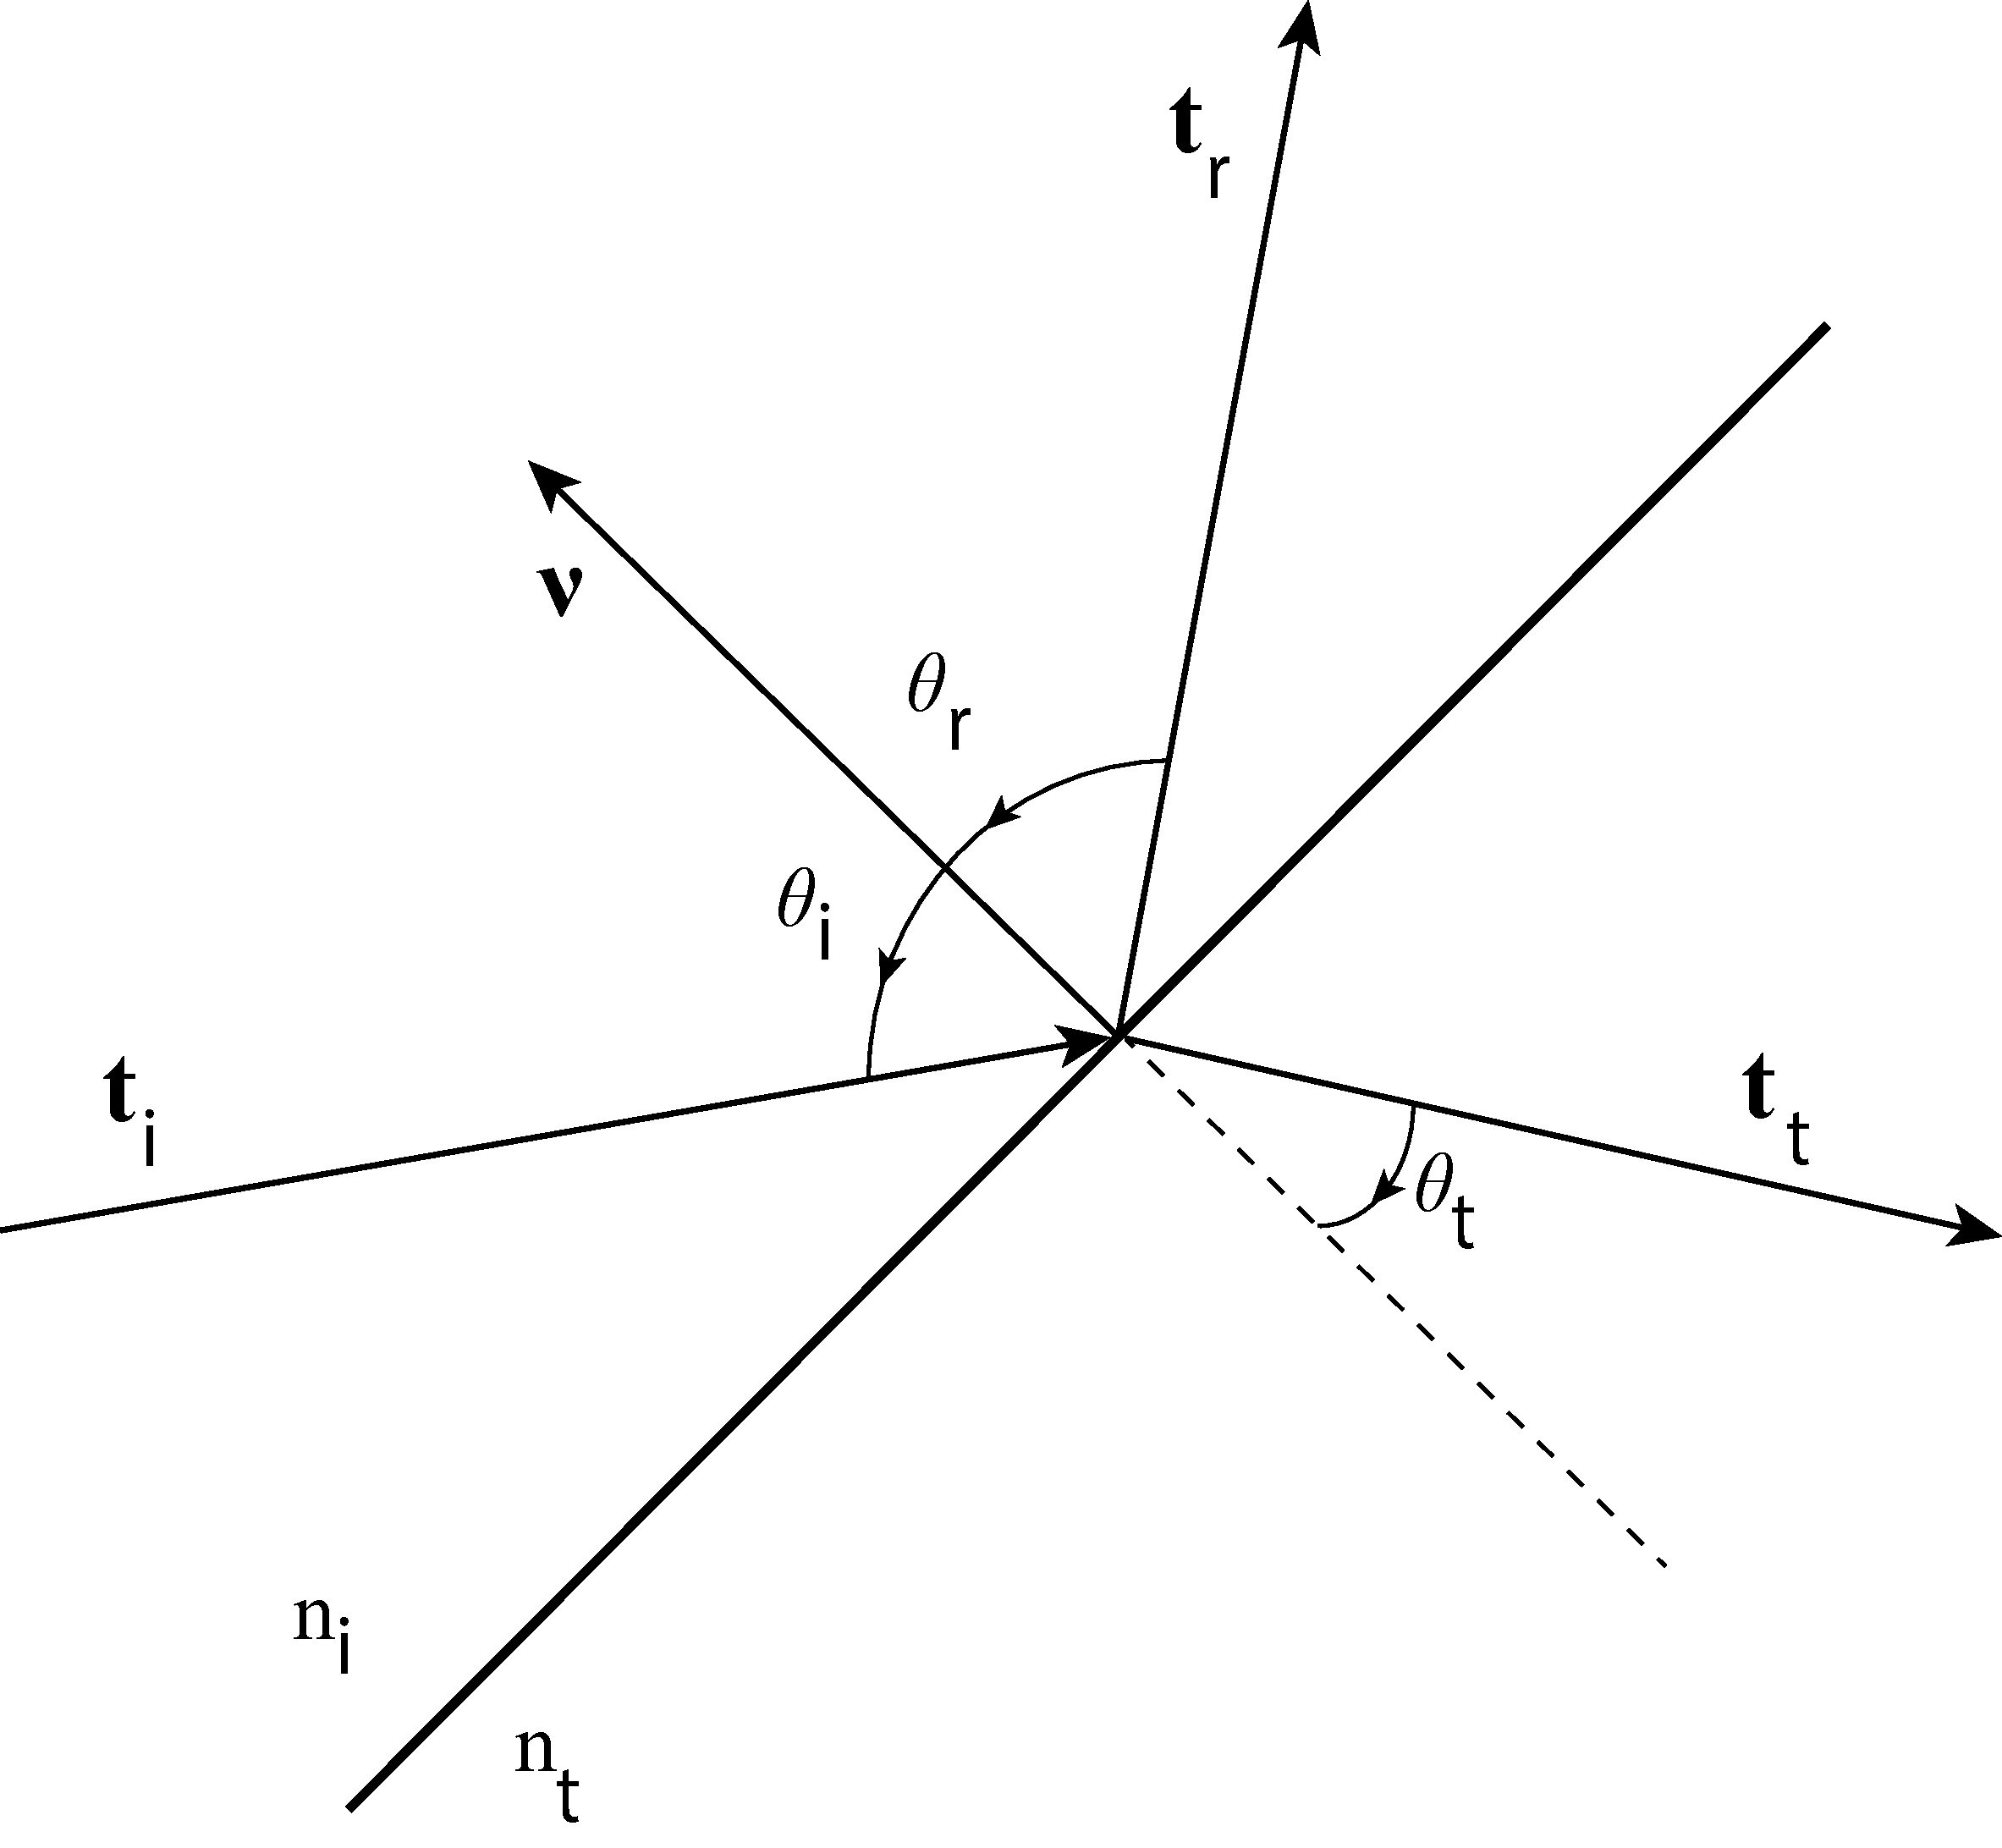
\includegraphics[width=8cm]{reflection}
     \end{center}
     \caption{\textbf{Propagation of a ray.} The ray travels through two materials with index of refraction $n_\textrm{i}$ and $n_\textrm{t}$.}% \bolsymbol{$\nu$} is the normal to the surface $A$ that the incident ray hits.
%$\vect{t}_i$, $\vect{t}_r$ and $\vect{t}_t$ are the direction vectors of the incident, reflected and refracted (or transmitted) ray, respectively. }}
%\myangle$_{i}$, \myangle$_{r}$ and \myangle$_{t}$ are the angles between \bolsymbol{$\nu$} and the incident, reflected and transmitted ray, respectively.}}
\label{fig:Snell}
 \end{figure}
\\ When a ray propagates through two different media, its direction changes according to the law of refraction. 
Indicating with $n_\textrm{i}$ the index of refraction of the medium in which the incident ray travels and with 
$n_\textrm{t}$ the index of refraction of the medium of the transmitted ray, the direction $\vect{t}_\textrm{t}$ of the transmitted ray is given by:
\begin{equation}\label{Refraction}
\vect{t}_\textrm{t} = n_{\textrm{i},\textrm{t}}\,\vect{t}_\textrm{i}+
\Big[\sqrt{1-n_{\textrm{i},\textrm{t}}^2+
n_{\textrm{i},\textrm{t}}^2(\boldsymbol{\nu}\boldsymbol{\cdot}\vect{t}_\textrm{i})^2}
-n_{\textrm{i},\textrm{t}}(\boldsymbol{\nu}\boldsymbol{\cdot}\vect{t}_\textrm{i}) \Big]\boldsymbol{\nu}\,,
\end{equation}
where $n_{\textrm{i},\textrm{t}}=n_\textrm{i}/n_\textrm{t}$ \cite{chaves2015introduction}.
While the direction of the normal $\boldsymbol{\nu}$ to the surface is not relevant for the computation of the direction of the reflected ray, in fact:
\begin{equation}
\vect{t}_\textrm{r} = \vect{t}_\textrm{i}-2(\vect{t}_\textrm{i}\boldsymbol{\cdot}\boldsymbol{\nu})\boldsymbol{\nu}= \vect{t}_\textrm{i}-2(\vect{t}_\textrm{i}\boldsymbol{\cdot}(-\boldsymbol{\nu}))(-\boldsymbol{\nu}), 
\end{equation}
for computing the direction of the refracted ray, we need to specify the direction of $\boldsymbol{\nu}$ which is usually chosen in such a way that the angle that it forms with the incident ray $\vect{t}_\textrm{i}$ is smaller than or equal to $\pi/2$. 
Considering the cross product of both the terms in Equation (\ref{Refraction}) and the normal $\boldsymbol{\nu}$ of the incident surface we obtain:
\begin{equation}
\vect{t}_\textrm{t}\times\boldsymbol{\nu} = n_{\textrm{i},\textrm{t}}(\vect{t}_\textrm{i}\times\boldsymbol{\nu})
\end{equation}
which leads to the Snell's law:
\begin{equation}\label{eq:snell}
n_\textrm{t}\sin(\myangle_\textrm{t}) = n_\textrm{i}\sin(\myangle_\textrm{i}).
\end{equation}
\\\indent
Note that Equation (\ref{Refraction}) is only valid for 
\begin{equation}\label{tir}
1-n_{\textrm{i},\textrm{t}}^2+n_{\textrm{i},\textrm{t}}^2(\boldsymbol{\nu}\boldsymbol{\cdot}\vect{t}_\textrm{i})^2\geq 0 
\end{equation} which implies that
\begin{equation}
\frac{n_\textrm{t}}{n_\textrm{i}}\geq \sqrt{1-(\boldsymbol{\nu}\boldsymbol{\cdot}\vect{t}_\textrm{i})^2},
\end{equation}
from which we obtain:
\begin{equation}
 %n_\textrm{t}\geq n_\textrm{i}\sqrt{1-\cos^2\myangle_\textrm{i}}= 
 n_\textrm{t}\geq n_\textrm{i} \sin\myangle_\textrm{i}\,.
\end{equation}
 The angle $\myangle_{\textrm{c}}$ for which the equality holds is
\begin{equation}\label{critical}
\myangle_{\textrm{c}} = \arcsin\Big(\frac{n_\textrm{t}}{n_\textrm{i}}\Big),
\end{equation} and it is called the critical angle \cite{chaves2015introduction}.
%Note that the condition $\frac{n_t}{n_i}<1$ is verified as in this case $\sin(\myangle_\textrm{i})<1$.
When the incident angle $\myangle_{\textrm{i}}$ is exactly equal to the critical angle $\myangle_{\textrm{c}}$, the square root in Equation (\ref{Refraction}) is zero and $\vect{t}_\textrm{t}\boldsymbol{\cdot}\boldsymbol{\nu})=0$, hence the transmitted ray propagates parallel to the refractive surface. 
When $\myangle_{\textrm{i}}>\myangle_{\textrm{c}}$ the light ray is no longer refracted but is only reflected by the surface. This phenomenon is called total internal reflection (TIR). When TIR occurs, $100\%$ of light is reflected and there is no refraction. Therefore, optical systems designed such that rays are reflected by TIR are very efficient. \\ \indent 
In general, light that hits an ordinary refractive surface can be both reflected and refracted. Every incident ray generates two rays when interacting with a surface. Each of the them carries a fraction of the total energy of the incident ray. Obviously, the sum of the reflected and transmitted energy equals the incident power.
The amount of energy transported by the reflected and the refracted ray is determined by the Fresnel's coefficients.
In the next paragraph an overview of the Fresnel equations is given.
\section{Fresnel equations}\label{sec:fresnel}
In order to derive Fresnel equations we need to describe light as an electromagnetic wave. 
It is therefore useful to study the light propagation from the perspective of electromagnetic theory which gives information about the incident, reflected and transmitted radiant flux density, which are denoted with $P_\textrm{i}$, $P_\textrm{r}$ and $P_\textrm{t}$, respectively.  
The electric field $\boldsymbol{\mathcal{E}}$ can be written as: 
\begin{equation}
\boldsymbol{\mathcal{E}}(\vect{x}, \mytime) = \boldsymbol{\mathcal{E}}_0(\vect{x} )e^{i( \vect{k}\boldsymbol{\cdot}\vect{x}-\omega \mytime)},
\end{equation}
where \vect{k} is the vector in the direction of the field propagation with modulus 
$|\vect{k}| = k$, \vect{x} is the position vector and $\mytime$ is the time. The amplitude $\boldsymbol{\mathcal{E}}_0(\vect{x})$ is constant in time and $\omega = \frac{c |\vect{k}|}{n}$ is the value of the angular frequency with $c$ the velocity of light and $n$ the index of refraction in which the wave is traveling, which is the ratio of $c$ and the speed of light $v$ in the material. Note that the angular frequency can be also written as $\omega = v\, k$ (in vacuum $n=1$ and $\omega=ck$). The value
$k = \frac{2\pi}{\lambda}$ is the wave number in vacuum, with $\lambda$ the wavelength. \\ \indent Similarly, the magnetic field has the form:
\begin{equation}
\boldsymbol{\mathcal{B}}(\vect{x}, \mytime) = \boldsymbol{\mathcal{B}}_0(\vect{x}) e^{i( \vect{k}\boldsymbol{\cdot} \vect{x}-\omega \mytime )}\,.
\end{equation}
The electric and magnetic fields satisfy the following relations:
\begin{subequations}
\begin{align}
\frac{\vect{k}}{|\vect{k}|} \boldsymbol{\times} \boldsymbol{\mathcal{E}} & = v \, \boldsymbol{\mathcal{B}}, \label{eq:electric_magnetic}\\
\frac{\vect{k}}{|\vect{k}|} \boldsymbol{\cdot}\boldsymbol{\mathcal{E}} &=0.
\end{align}
\end{subequations}
% Say right hand system
\\ \indent Light can be seen as an electromagnetic wave consisting of an electric field $\boldsymbol{\mathcal{E}}$ and a field $\boldsymbol{\mathcal{B}}$ which propagates always perpendicular to $\boldsymbol{\mathcal{E}}$ and $\vect{k}$ (see Equation (\ref{eq:electric_magnetic})). By convention, the direction of the electric field $\boldsymbol{\mathcal{E}}$ \cite{feynman1964feynman} with respect to the incident plane defines the \textit{polarization} of an electromagnetic wave. The direction of $\boldsymbol{\mathcal{E}}$ is given by the incident and reflected rays as is shown in Figure \ref{fig:planeofincidence}. \\
\indent Fresnel equations were introduced to describe the effect of an incident wave when encountering an interface located between two media having a different indices of refraction. In particular Fresnel coefficients determine the fractions of transmitted and reflected energy.  
In the following we provide Fresnel coefficients and we briefly explain their physical interpretation. 
We refer the reader to \cite{born2013principles, hecht1998hecht, feynman2011feynman} for more details. To derive Fresnel equations the polarization of light must be taken into account.
\\ \indent Light is said to be \textit{polarized} if the electric field oscillates in a single plane. Light is \textit{unpolarized} when the direction of this electric field changes randomly in time.
\begin{figure}[t]
 \label{fig:planeofincidence}
     \begin{center}
     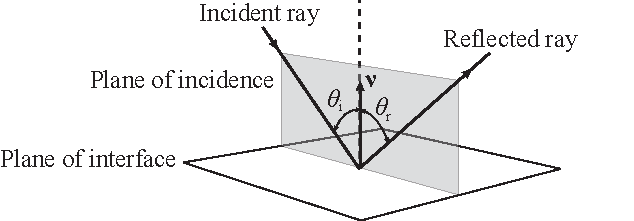
\includegraphics[width=10cm]{plane_of_incidence1}
     \end{center}
     \caption{\textbf{Light ray that hits a mirror located on the reflecting plane.} The incident and the reflected ray are coplanar to the normal to the mirror. The plane of incidence is spanned by the reflected and the refracted rays. The plane of interface is perpendicular to the plane of incidence.}
\label{fig:planeofincidence}
 \end{figure}
The light polarization can be classified into three different kinds of polarization:
\begin{itemize}
\item \textit{Linear polarization}: The electric filed is confined to a single plane perpendicular along the direction of propagation;
\item \textit{Circular polarization}: The electric field describes a circle around the direction of polarization;
\item \textit{Elliptic polarization}: The electric field describes an ellipse around the direction of polarization.
\end{itemize}
Any form of light can be defined by two ortogonal linear polarization.
Hence, the two following cases of light polarization are considered: 
\begin{enumerate}
\item $\boldsymbol{\mathcal{E}}$ is perpendicular to the plane of incidence and, therefore $\boldsymbol{\mathcal{B}}$ is parallel to it (see Figure \ref{fig:electric_field}). In this case light is said to be \textit{s-polarized} (from the German word \textit{senkrecht}).
\item $\boldsymbol{\mathcal{E}}$ is parallel to the plane of incidence and, therefore $\boldsymbol{\mathcal{B}}$ is perpendicular it (see Figure \ref{fig:electric_field_p}). In this case light is said to be \textit{p-polarized} (from the German word \textit{parallel}).
\end{enumerate}
\begin{figure}[h]
 \label{fig:electric_field}
     \begin{center}
     \includegraphics[width=8cm]{electric_field}
     \end{center}
     \caption{\textbf{Propagation of an electromagnetic wave where $\boldsymbol{\mathcal{E}}$ is perpendicular to the incident plane.} The components of $\boldsymbol{\mathcal{E}}$ are indicated with the green circles.
The components of $\boldsymbol{\mathcal{B}}$ are indicated with red arrows.}
\label{fig:electric_field}
 \end{figure}
\begin{figure}[h]
 \label{fig:electric_field_p}
     \begin{center}
     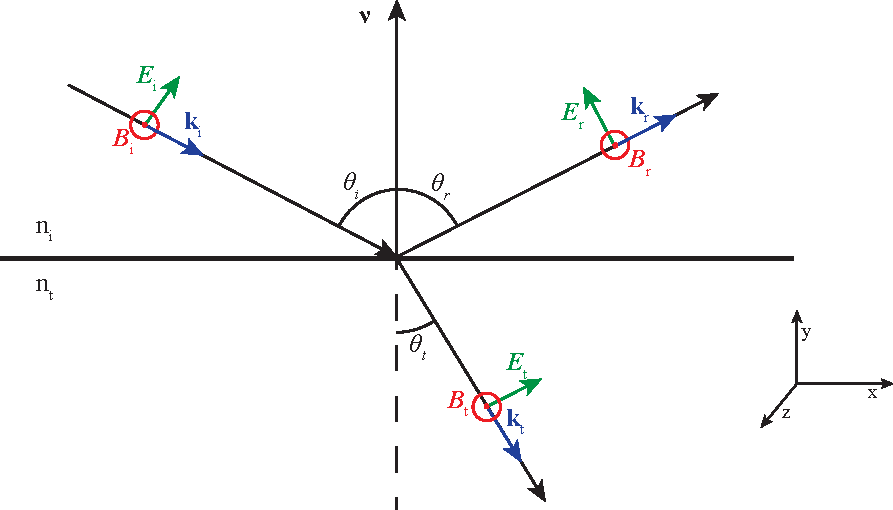
\includegraphics[width=8cm]{electric_field_p}
     \end{center}
 \caption{\textbf{Propagation of an electromagnetic wave where $\boldsymbol{\mathcal{E}}$ is parallel to the incident plane.} The components of $\boldsymbol{\mathcal{B}}$ are indicated with the red circle.
%, they are in the $(\variabile{x},\variabile{z})$ plane and they are oriented in the positive direction of $\variabile{z}$. 
The components of $\boldsymbol{\mathcal{E}}$ are indicated with greed arrows.}
%and they are located in the $(\variabile{x}, \variabile{z})$ plane.}
\label{fig:electric_field_p}
 \end{figure}
Energy conservation gives the boundary conditions of the electromagnetic field at the plane of the interface (perpendicular to the incident plane), from which the Fresnel coefficients are derived. They are defined in both case $1$ and case $2$. Since the mathematical formulation is similar for the two cases, in the following we explain in details the computation of the Fresnel coefficients only for s-polarized light (case $1$).\\ 
\indent For s-polarized light the tangential components of $\boldsymbol{\mathcal{E}}$ and $\boldsymbol{\mathcal{B}}/\mu$ across the boundary between the two different media must be continuous. From now on, all quantities defined in the medium of the incident, reflective and transmitted light are indicated with the subscripts \textrm{i}, \textrm{r} and \textrm{t}, respectively. The continuity of the tangential component of $\boldsymbol{\mathcal{E}}$ leads to:
\begin{equation}\label{Econservation}
|\boldsymbol{\mathcal{E}}_{0\textrm{i}}|+|\boldsymbol{\mathcal{E}}_{0\textrm{r}}|= |\boldsymbol{\mathcal{E}}_{0\textrm{t}}|,
\end{equation} 
%where we have indicated with $\mathcal{E}_{0\textrm{i}}$, $\mathcal{E}_{0\textrm{r}}$ and $\mathcal{E}_{0\textrm{t}}$
%the magnitudes of $\boldsymbol{\mathcal{E}}_{0\textrm{i}}$, $\boldsymbol{\mathcal{E}}_{0\textrm{r}}$ and $\boldsymbol{\mathcal{E}}_{0\textrm{t}}$, respectively.
while the continuity of the tangential component of $\boldsymbol{\mathcal{B}}/\mu$ gives:
\begin{equation}\label{Bconservation}
-\frac{|\boldsymbol{\mathcal{B}}_{0,\textrm{i}}|}{\mu_\textrm{i}}\cos\myangle_{\textrm{i}}+\frac{|\boldsymbol{\mathcal{B}}_{0,\textrm{r}}|}{\mu_\textrm{r}}\cos\myangle_{\textrm{r}} = 
-\frac{|\boldsymbol{\mathcal{B}}_{0,\textrm{t}}|}{\mu_\textrm{t}}\cos\myangle_{\textrm{t}},
\end{equation}
where the sign convention is chosen as illustrated in Figure \ref{fig:electric_field}.
%where we have indicated with $\mathcal{B}_{\textrm{i}}$, $\mathcal{B}_{\textrm{r}}$ and $\mathcal{B}_{\textrm{t}}$
%the absolute values of $\boldsymbol{\mathcal{B}}_{\textrm{i}}$,$\boldsymbol{\mathcal{B}}_{\textrm{r}}$ and $\boldsymbol{\mathcal{B}}_{\textrm{t}}$, respectively.
Since $|\boldsymbol{\mathcal{B}}| = |\boldsymbol{\mathcal{E}}|/v$, Equation (\ref{Bconservation}) can be written as 
\begin{equation}
\frac{1}{\mu_{\textrm{i}}v_{\textrm{i}}}(|\boldsymbol{\mathcal{E}}_{0,\textrm{i}}|-|\boldsymbol{\mathcal{E}}_{0,\textrm{r}}|)\cos\myangle_{\textrm{i}} = \frac{1}{\mu_{\textrm{t}}v_{\textrm{t}}}|\boldsymbol{\mathcal{E}}_{0,\textrm{t}}|\cos\myangle_{\textrm{t}},
\end{equation}
where we employed the fact that $v_{\textrm{i}}= v_{\textrm{r}}$, and $\myangle_{\textrm{i}}= \myangle_{\textrm{r}}$. 
Since $n = c/v$, the previous equation becomes:
\begin{equation}
\frac{n_{\textrm{i}}}{\mu_{\textrm{i}}}(|\boldsymbol{\mathcal{E}}_{0\textrm{i}}|-|\boldsymbol{\mathcal{E}}_{0\textrm{r}}|)\cos\myangle_{\textrm{i}} = \frac{n_{\textrm{t}}}{\mu_{\textrm{i}}}|\boldsymbol{\mathcal{E}}_{0\textrm{t}}|\cos\myangle_{\textrm{t}}.
\end{equation}
Most often used optical materials are non-magnetic, hence we assume that $\mu_{\textrm{i}}=\mu_{\textrm{t}}=\mu_{0}$ \cite{lvovsky2013fresnel}. Employing Equation (\ref{Econservation}) we arriving at the Fresnel coefficient for s-polarized light:
\begin{equation} \label{Fresnel_perpendicular}
\begin{split}
r_{s} & =\frac{|\boldsymbol{\mathcal{E}}_{0 \textrm{r}}|_{s}}{|\boldsymbol{\mathcal{E}}_{0\textrm{i}}|_s} = 
\frac{n_\textrm{i}\cos\myangle_\textrm{i}-n_\textrm{t} \cos\myangle_\textrm{t}}{n_\textrm{i}
\cos\myangle_\textrm{i}+n_\textrm{t}\cos\myangle_\textrm{t}},\\
t_{s} & = \frac{|\boldsymbol{\mathcal{E}}_{0 \textrm{t}}|_s}{|\boldsymbol{\mathcal{E}}_{0\textrm{i}}|_s} 
=\frac{2n_\textrm{i}\cos\myangle_\textrm{i}}{n_\textrm{i}\cos\myangle_\textrm{i}+n_\textrm{t}\cos\myangle_\textrm{t}},\\
\end{split}
\end{equation}
where the subscript $s$ is used to remind the reader that we are considering s-polarized light. The coefficients $r_s$ and $t_s$ are perpendicular components of the amplitude coefficients of the reflected and transmitted light:
\begin{equation}
\begin{split}
r & =\frac{|\boldsymbol{\mathcal{E}}_{0 \textrm{r}}|}{|\boldsymbol{\mathcal{E}}_{0\textrm{i}}|}, \\
t & =\frac{|\boldsymbol{\mathcal{E}}_{0 \textrm{t}}|}{|\boldsymbol{\mathcal{E}}_{0\textrm{i}}|}.
\end{split}
\end{equation}
Using Snell's law (Equation (\ref{eq:snell})) the first pair of Fresnel equation become:
\begin{equation} \label{simple_Fresnel}
\begin{split}
r_{s} & = -\frac{\sin(\myangle_i-\myangle_t)}{\sin(\myangle_i+\myangle_t)},\\
t_{s} & = -\frac{2\sin \myangle_t \cos \myangle_i}{\sin(\myangle_i+\myangle_t)}\,.
\end{split}
\end{equation}
\indent A similar argument for the p-polarized light leads to the calculation of the parallel components $r_p$ and $t_p$ of $r$ and $t$. 
The boundaries conditions for the electric and magnetic field:
\begin{subequations}
\begin{align}
|\mathcal{E}_{0 i}|\cos(\myangle_{\textrm{i}}) - |\mathcal{E}_{0 r}|\cos(\myangle_{\textrm{r}}) &= |\mathcal{E}_{0 t}|\cos(\myangle_{\textrm{t}})\\
|\mathcal{B}_{0 i}| + |\mathcal{B}_{0 r}| &= |\mathcal{B}_{0 t}|
\end{align}
\end{subequations}
leads to the second pair of Fresnel equations:
\begin{equation}\label{Fresnel_parallel}
\begin{split}
r_{p} & = \frac{|\boldsymbol{\mathcal{E}}_{0 \textrm{r}}|_{p}}{|\boldsymbol{\mathcal{E}}_{0\textrm{i}}|_p} = \frac{n_t\cos\myangle_i-n_i \cos\myangle_t}{n_i \cos\myangle_t+n_t\cos\myangle_i},\\
t_{p} & =\frac{|\boldsymbol{\mathcal{E}}_{0 \textrm{t}}|_{p}}{|\boldsymbol{\mathcal{E}}_{0\textrm{i}}|_p} =  \frac{2n_i\cos\myangle_i}{n_i\cos\myangle_t+n_t\cos\myangle_i}\,,
\end{split}
\end{equation}
and their simplified versions reduce to:
\begin{equation} \label{simple_Fresnel}
\begin{split}
r_{p} & =  \frac{\tan(\myangle_i-\myangle_t)}{\tan(\myangle_i+\myangle_t)},\\
t_{p} & = \frac{2\sin \myangle_t \cos \myangle_i}{\sin(\myangle_i+\myangle_t)\cos(\myangle_i- \myangle_t)}.
\end{split}
\end{equation}
Furthermore, it can be checked that
 \begin{equation}
\begin{split}
t_s-r_s &= 1, \\
t_p+r_p &=  1.
\end{split}
\end{equation}
\\ \indent The amplitude coefficients are shown in Figure \ref{fig:coefficients} for the case in which light travels from a less dense to a more dense medium, i.e. $n_\textrm{i}<n_\textrm{t}$ where $n_{\textrm{i}}= 1$ and $n_{\textrm{t}}=1.5$. 
In Figure \ref{fig:coefficients2} the reflection coefficients are shown for the case in which $n_\textrm{i}>n_\textrm{t}$ with $n_{\textrm{i}}= 1.5$ and $n_{\textrm{t}}=1$. Note from Figure \ref{fig:coefficients} that $r_p$ approaches to $0$ when $\myangle_i$ approaches to $\myangle_p$ and it gradually decreases reaching $-1$ for an incident angle $\myangle_i=90^\circ$. The angle $\myangle_p$ is called \textit{Brewster's angle} or polarization angle as only the component perpendicular to the incident plane is reflected at that angle and therefore light is perfectly polarized. Similarly, Figure \ref{fig:coefficients2} shows that $r_p=0$ for $\myangle_i= \myangle_{p\prime}$. It can be show that $\myangle_p+ \myangle_{p\prime}= 90^\circ$. Both $r_p$ and $r_s$ reach $1$ when $\myangle_i= $ $\myangle_c$. $\myangle_c$ is called the critical angle. Light that hits the incident plane with an incident angle equal to or greater than $\myangle_{c}$ is totally reflected back and no transmitted light is observed. This phenomenon is called total internal reflection. 
\begin{figure}[h]
  \begin{minipage}[h]{0.48\textwidth}
    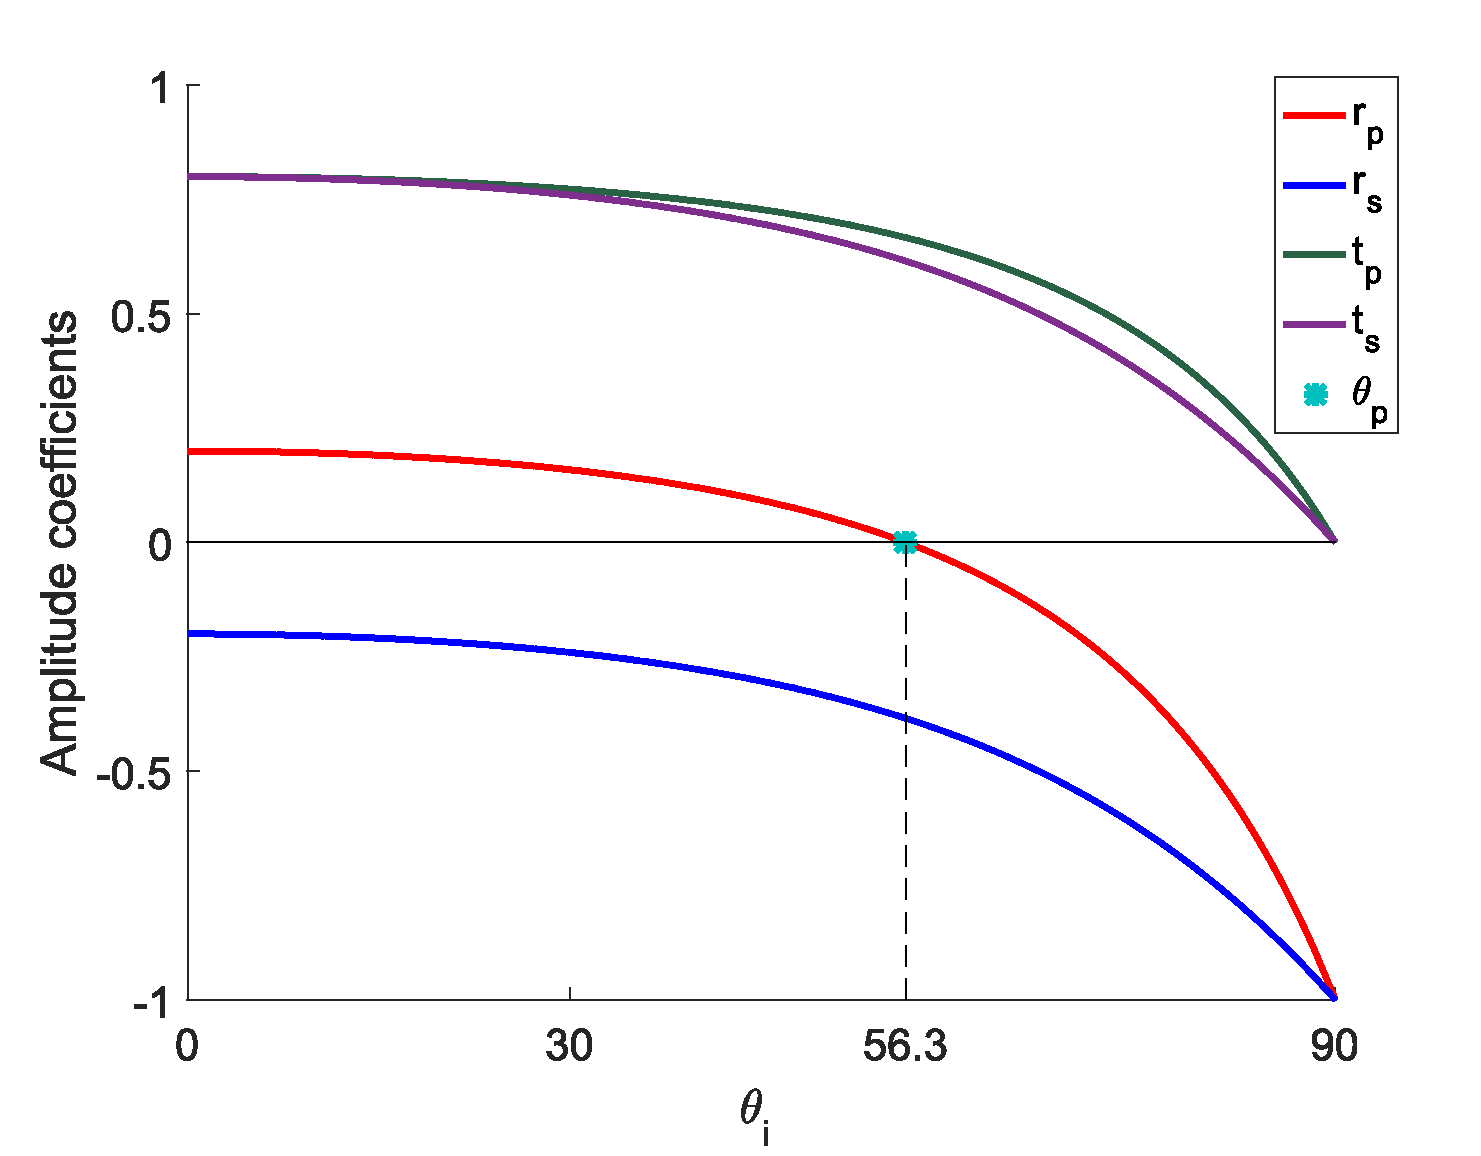
\includegraphics[width=\textwidth]{amplitude_coefficients}
    \caption{\textbf{Amplitude coefficients of reflection and transmission.} $n_\textrm{t}<n_\textrm{i}$
($n_\textrm{t} = 1$ and $n_\textrm{i}=1.5$). $\myangle_p = 56.3^\circ$ is the polarization angle.}
    \label{fig:coefficients}
  \end{minipage}\hfill
  \begin{minipage}[h]{0.48\textwidth}
    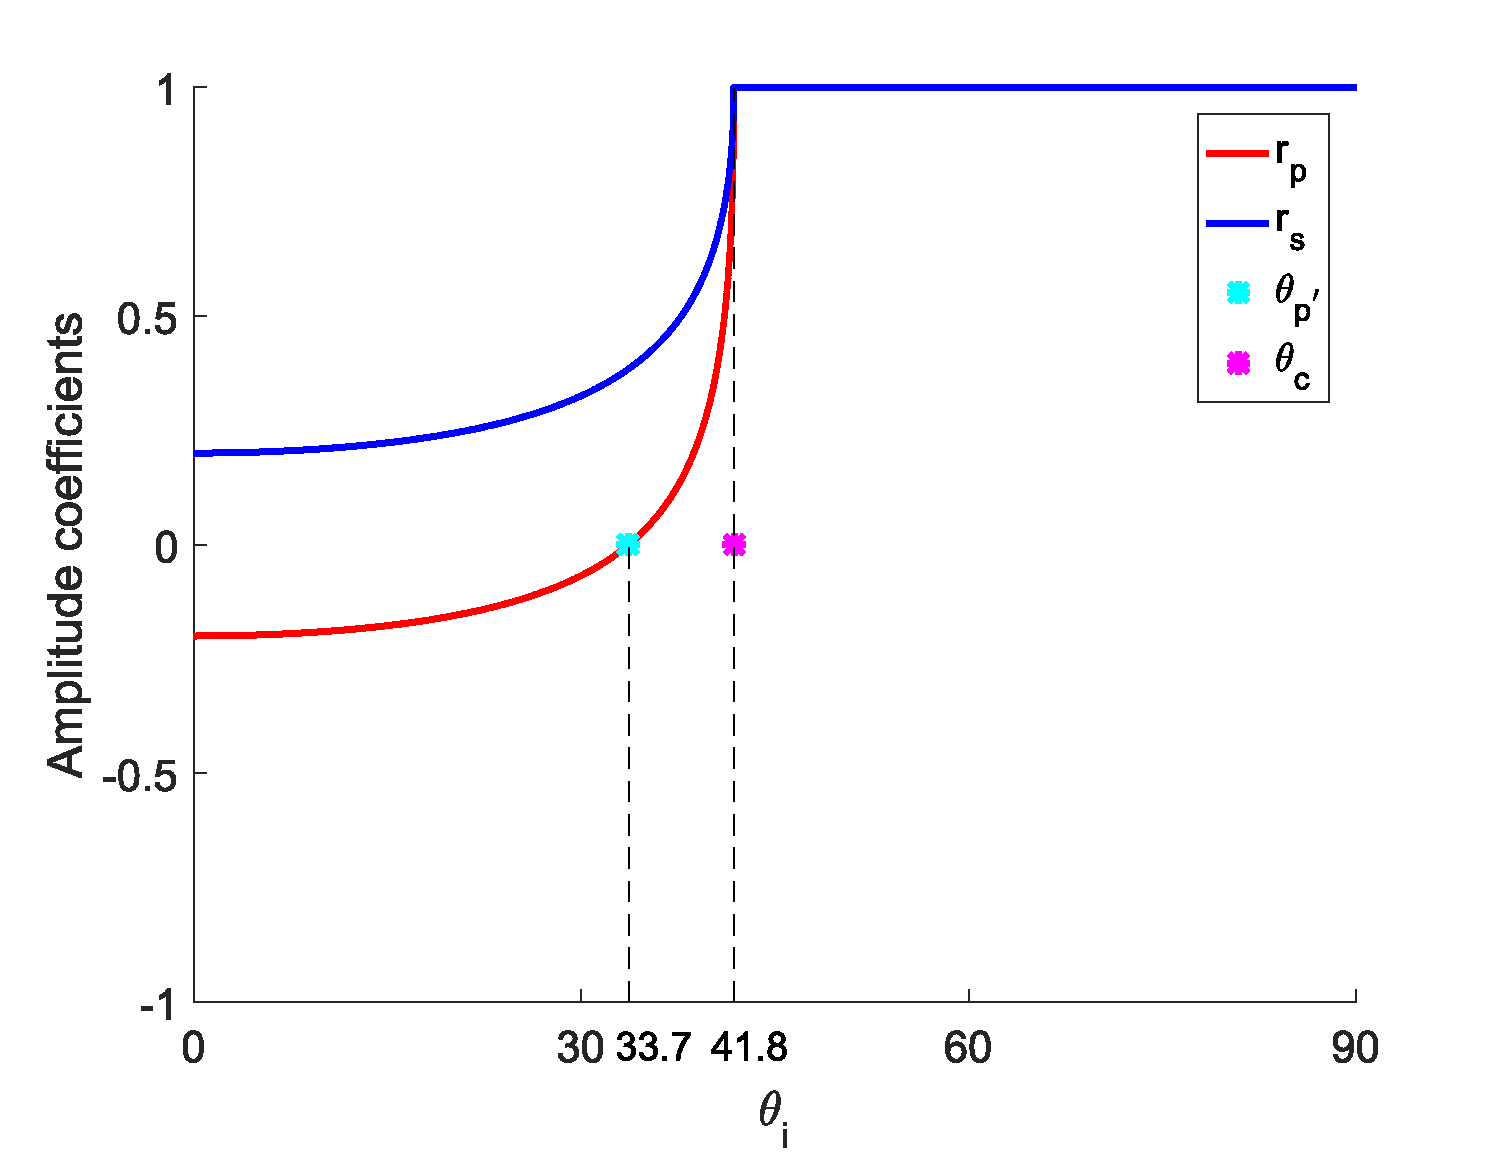
\includegraphics[width=\textwidth]{rprs}
    \caption{\textbf{Amplitude reflection coefficients.} $n_\textrm{t}>n_i$
($n_\textrm{t} = 1.5$ and $n_\textrm{i}=1$). $\myangle_{p\prime}= 33.7^\circ$ is the polarization angle and $\myangle_c= 41.8^\circ$ is the critical angle.}
   \label{fig:coefficients2}
 \end{minipage}
\end{figure}\\
%\indent The  we introduce the Poynting vector \vect{P} that defines the energy flux of an electromagnetic field. 
%It is measured in $[\textrm{W}/\textrm{m}^2]$, and it is given by:
%\begin{equation}
%\vect{P} = \frac{1}{\mu}\Big(\boldsymbol{\mathcal{E}}\boldsymbol{\times} \boldsymbol{\mathcal{B}}\Big),
%\end{equation}
%where $\mu = \frac{1}{\varepsilon v^2}$ is the permeability and $\varepsilon$ the permittivity of the medium.
% In the following, the parameters for vacuum are indicated with the subscript $0$. Optical rays are perpendicular to the wave front of an electromagnetic wave and parallel to the Poynting vector \cite{jones2015optical}.
\indent It can be useful to define the reflection and transmission coefficients in terms of the irradiance (or radiant flux density) $P$ rather than amplitudes of the electric field. For a wave of amplitude $|\mathcal{E}_0|$ propagating in a non-magnetic medium with a refractive index $n$, $P$ is given by:
%Therefore, defining the average of the vector \vect{P} over the time as:
%\begin{equation}
%\langle \vect{P} \rangle_T = \frac{1}{T}\int_0^T \vect{P}\textrm{d}T
%\end{equation}
%we can write the irradiance $E$ as:
\begin{equation}
P = \frac{c\, n \, \varepsilon_0}{2}|\boldsymbol{\mathcal{E}_0}|^2 \,.
\end{equation}
For a beam of light that hits a surface such that an area $A$ is illuminated,
$P$ is the average energy that crosses in unit time a unit area $A$ perpedicular to the direction of the energy flow.
We indicate with $P_{\textrm{i}}$, $P_{\textrm{r}}$ and $P_{\textrm{t}}$ the incident, reflected and transmitted flux densities, respectively.
The energy per unit time for the incident, reflected and transmitted beams are 
$P_\textrm{
i} A\cos\myangle_\textrm{i}$ $P_\textrm{r} A\cos\myangle_\textrm{r}$ and 
$P_\textrm{t} A\cos\myangle_\textrm{t}$, respectively. % as is shown in Figure \ref{}
The reflectance $\mathcal{R}$ is the ratio of the reflected power to the incident power:
\begin{equation}\label{reflectance}
\mathcal{R} = \frac{P_\textrm{r}\cos\myangle_r}{P_\textrm{i}\cos\myangle_\textrm{i}} = \frac{|\boldsymbol{\mathcal{E}}_{0 \textrm{r}}|^2}{|\boldsymbol{\mathcal{E}}_{0 \textrm{i}}|^2} = r^2
\end{equation}
where the second equality holds because $v_{\textrm{i}}= v_{\textrm{t}}$, $\varepsilon_{\textrm{i}} = \varepsilon_{\textrm{t}}$ and $\myangle_{\textrm{i}} = \myangle_{\textrm{t}}$.
Similarly, the transmittance $\mathcal{T}$ is the ratio between the transmitted to the incident power:
\begin{equation}\label{transmittance}
\mathcal{T} = \frac{P_\textrm{t} \cos\myangle_\textrm{t}}{P_\textrm{r}\cos\myangle_\textrm{r}} = \frac{n_\textrm{t} \cos\myangle_\textrm{t}}{n_\textrm{t} \cos\myangle_\textrm{i}}\frac{|\boldsymbol{\mathcal{E}}_{0 \textrm{t}}|^2}{\boldsymbol{|\mathcal{E}}_{0 \textrm{i}}|^2} = \frac{n_\textrm{t} \cos\myangle_\textrm{t}}{n_\textrm{t} \cos\myangle_\textrm{i}} t^2\,.
\end{equation}
Employing total energy conservation, that is:
\begin{equation}
P_\textrm{i} A\cos\myangle_\textrm{i} = P_\textrm{r} A\cos\myangle_\textrm{r}+P_\textrm{t} A\cos\myangle_\textrm{t},
\end{equation}
we can easily prove that:
\begin{equation}
\mathcal{R}+\mathcal{T}=1\,.
\end{equation}
 The parallel and perpendicular components of $\mathcal{R}$ and $\mathcal{T}$ are:
\begin{equation}\label{Fresnel_pands}
\begin{split}
\mathcal{R}_p& =  {r_p^2},\\
\mathcal{T}_p &=  \frac{n_t \cos\myangle_t}{n_t \cos\myangle_i}t_p^2,\\
\mathcal{R}_s &=  r_s^2,\\
\mathcal{T}_s &= \frac{n_t \cos\myangle_t}{n_t \cos\myangle_i}t_s^2.\\
\end{split}
\end{equation}
It can be show that
\begin{equation}
\begin{split}
\mathcal{R}_s+\mathcal{R}_p &= 1,\\
\mathcal{T}_s+\mathcal{T}_p &=1\,.
\end{split}
\end{equation}
For normal incidence, i.e. $\myangle_i = 0$, the incident plane is not defined and there is no distinction between the perpendicular and the parallel components of $\mathcal{R}$ and $\mathcal{T}$. As a consequence, (\ref{Fresnel_pands}) leads to:
\begin{equation}\label{eq:fresnel_pands2}
\begin{split}
\mathcal{R} &= \mathcal{R}_p = \mathcal{R}_s = \Bigg(\frac{n_i-n_t}{n_t+n_i}\Bigg)^2, \\
\mathcal{T} &= \mathcal{T}_p = \mathcal{T}_s = \frac{4n_i n_t}{(n_t+n_i)^2}\,.
\end{split}
\end{equation}
\indent %In two dimensions light hits lines instead of surfaces. Therefore only the plane of incidence is defined and it has no sense to consider separately the parallel and the perpendicular polarization. 
Many common light sources such as the sun, halogen lighting, LED spotlights, and incandescent bulbs produce unpolarized light. 
In this case, light can be represented by the sum of two ortogonal states. If $\mathcal{R}_p = \mathcal{R}_s$ and $\mathcal{T}_p = \mathcal{T}_s$, then the amount of energy in one of the two polarization states is the same of that in the other \cite{hecht1998hecht}.
Hence it is reasonable to take as reflectance and transmittance the average of the quantities calculated considering first p-polarized light and then $s$-polarization, that is:
\begin{equation}\begin{split}
\mathcal{R} &= \frac{\mathcal{R}_p+ \mathcal{R}_s}{2},\\
\mathcal{T} &= \frac{\mathcal{T}_p+ \mathcal{T}_s}{2}.
\end{split}
\label{eq:RandTin2D}
\end{equation}
The reflectance $\mathcal{R}$ and the transmittance $\mathcal{T}$ give the fraction of the power of energy reflected and transmitted at every interaction of a light ray with a Fresnel surface.
 \\
\indent With this overview we conclude this chapter. The notions given in Section \ref{sec:photometry} will be used in the entire thesis as our goal is to study the distribution of light at the target of some optical systems. In particular we will focus on the computation of the output intensity distribution. The reflection and refraction laws explained in Section \ref{sec:reflection} are needed to determine how the optical system changes the ray's direction every time that it hits a surfaces (or a line in the two-dimensional case). In Chapters \ref{chap:raytracing}-\ref{chap:raymapping2} only systems where the reflection and refraction laws play a role are considered. Systems with Fresnel reflection are treated in the last chapter. The amount of reflected and transmitted light is calculated using the Fresnel equations. In our simulations we consider the general case of unpolarized light. 

\chapter{Ray tracing}\label{chap:raytracing}
Optical ray tracing is a tool to calculate the transport of light within optical systems.
Given an optical system and a set of rays at the source, ray tracing relates the emitted light with its output distribution. 
The influence of diffraction on the transport of a ray is neglected. \\ \indent
Although the method can be implemented for two or more dimensions and for any optical system, here we consider the two-dimensional case only. 
We will thus refer to optical lines instead of optical surfaces.
The two-dimensional case has some limitations. For example, it may not identify skew rays that are turned back by the system, with the consequence that a 2D analysis cannot guarantee a proper treatment of non-meridional rays in 3D. 
Nevertheless, the two-dimensional case is particularly relevant because it is a good test case to demonstrate the performance of new methods.
Optical designers often start with 2D systems, where only the meridional plane is taken into account because it gives a good prediction of the target distribution of the rays
(see \cite{winston2005nonimaging}, chapter $4$).
% Why there are alternatives
\section{Ray tracing for two-dimensional optical systems}\label{sec:raytracing}
The purpose of ray tracing applied to non-imaging optical systems is to calculate the target rays distribution given an optical system and an initial distribution of the rays at the source.
Light rays are straight lines and they are reflected or refracted by the optical components of a system.
Every ray emitted from the source is followed until it reaches the target.  
The ray tracing procedure is constructed such that the position and the direction of the rays are calculated on every optical line that they hit. \\ \indent
Given a Cartesian coordinate system $(\variabile{x}, \variabile{z})$, a two-dimensional optical system symmetric with respect to the $\variabile{z}$-axis is defined.
Hence, we assume that the optical axis coincides with the $\variabile{z}$-axis.
The optical system is formed by a source \point{S}, a target  \point{T} and some optical components labeled with indexes $\lineai$ where $\lineai \in \{2, \cdots, \nline-1\}$ and $\nline$
 indicates the number of lines that form the system. \point{S} and \point{T} are indicated with the indexes $1$ and $\nline$, respectively.
The index of refraction of the medium in which line $\lineai$ is located is indicated with $\n_\lineai$.
Every ray emitted by \point{S} (line $1$) can hit some optical components $\lineai\in\{2, \cdots, \nline -1\}$ before reaching \point{T} (line $\nline$).
The intersection point of the rays with line $\lineai$ are $(\variabile{x}_\lineai, \variabile{z}_\lineai)_{\lineai =1, \cdots, \nline}$ and, $\vect{s}_\lineai= (-\sin \optangle_\lineai, \cos \optangle_\lineai)$ indicates the direction vector of the rays that leave $\lineai$,
with $\optangle_\lineai$ the angle that the ray forms with respect to the optical axis measured counterclockwise. As we consider only forward rays, the angles
$\optangle_\lineai\in (-\pi/2, \pi/2)$.
Therefore, a ray segment between $(\variabile{x}_\lineai, \variabile{z}_\lineai)$ and $(\variabile{x}_\lineaj, \variabile{z}_\lineaj)$
with $\lineaj\neq\lineai$ is parameterized in real space by:
\begin{equation}
\label{parametrization}
\vect{r}(\variabile{s})=
\left( \begin{array}{cc}
\variabile{x}_\lineai-\variabile{s}\sin\optangle_\lineai \\
\variabile{z}_\lineai+\variabile{s}\cos\optangle_\lineai\end{array} \right) \qquad \quad 0< \variabile{s}\leq \variabile{s}_{\textrm{max}}\,,
\end{equation}
where \variabile{s} denotes the arc-length and $\variabile{s}_{\textrm{max}}$ is the maximum value that it can assume.
Figure \ref{fig:cup} shows an example where a single ray is traced inside a very simple optical system, the so-called two-faceted cup.
\begin{figure}[t]
\label{fig:cup}
  \begin{center}
%\vspace{-1.5cm}
  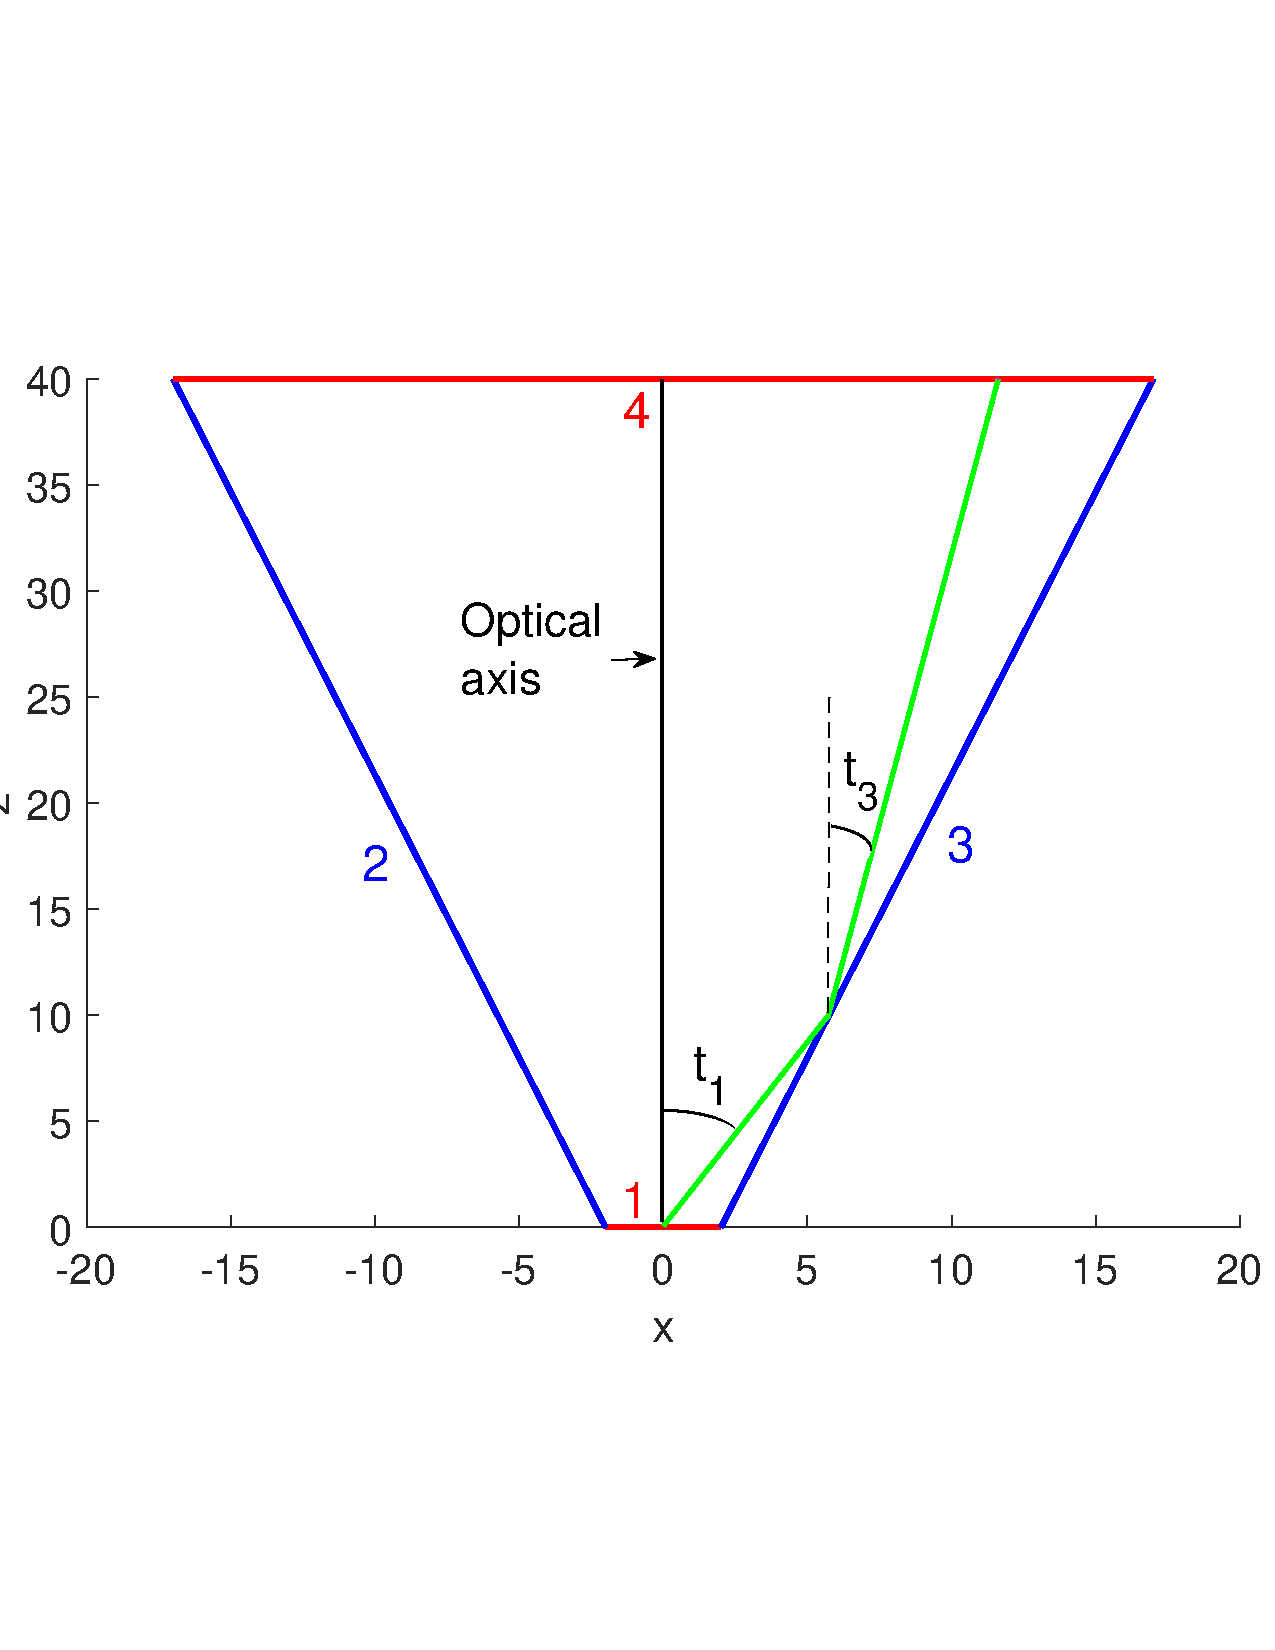
\includegraphics[width=6.7cm]{cup.pdf}
  \end{center}
%\vspace{-2cm}
  \caption{\textbf{Shape of the two-faceted cup.}  Each line of the system is labeled with a number.
   The source \point{S}$= [-2,2]$ (line number $1$) is located on the $\variabile{x}$-axis.
   The target \point{T}$= [-17, 17]$ (line $4$) is parallel to the source and is located at a height $\variabile{z}= 40$.
   The left and right reflectors (line $2$ and $3$) connect the source with the target.}
  \label{fig:cup}
\end{figure}
The light source \point{S}$= [-\variabile{a}, \variabile{a}]$ (line $1$) and the target \point{T}$~=~ [-\variabile{b}, \variabile{b}]$ (line $4$) are two segments normal to the \variabile{z}-axis, where $\variabile{a}=2$ and $\variabile{b}=17$.
The left and right reflectors (line $2$ and $3$) are oblique segments that connect the source and the target.
All the optical lines $\lineai \in \{1, \cdots, 4\}$  are located in air, thus the refractive index is $\n_{\lineai}=1$ for every $\lineai$. \\ \indent
In order to compute the target photometric variables, we need to know how the optical system influences the direction of the rays when they hit an optical line.
Ray tracing relates the position coordinates
 $ (\variabile{x}_1, \variabile{z}_1)$ and the direction vector $\vect{s}_1$ of every ray at the source $\point{S}$ with the corresponding position $(\variabile{x}_\nline, \variabile{z}_\nline)$ and direction $\vect{s}_\nline$
 at the target $\point{T}$. In the following we will often use the target coordinates of the rays thus, to simplify the notation, we do not write the subscript $\nline$ for the target coordinates. We rather write $(\variabile{x},\variabile{z})$ instead of $(\variabile{x}_\nline, \variabile{z}_\nline)$,  $\optangle$ instead of $\optangle_\nline$ and $\vect{s}$ instead of $\vect{s}_{\nline}$ for the target coordinates.
The ray tracing algorithm can be outlined as follows:
\begin{enumerate}
\item Indicating with $\variabile{i}$ the index of the line that rays leave, start considering a ray thet leaves the source $\point{S}$ (line \variabile{i}=1);
 \item Consider a ray with position coordinates $(\variabile{x}_\variabile{i}, \variabile{z}_\variabile{i})$ and direction $\vect{s}_\variabile{i}~=~(-\sin \optangle_\variabile{i}, \cos \optangle_\variabile{i})$, use equation ($\ref{parametrization}$) to implement the ray parametrization $\vect{r}(\variabile{s})$;
\item Compute the coordinates $(\variabile{x}_\variabile{k}, \variabile{z}_\variabile{k})_{\variabile{k} = 1\cdots, \nline}$ of the intersection point of the parameterized ray $\vect{r}(\variabile{s})$ with all the lines that it crosses
\begin{itemize}
\item[a)] if the shape of the lines is described by an explicit equation, the intersection points are determined analytically;
\item[b)] if there is no analytic description for the optical lines, the intersections need to be determined using iterative methods;
\end{itemize}
\item  Determine the minimal positive distance between $(\variabile{x}_\variabile{i}, \variabile{z}_\variabile{i})$ and $(\variabile{x}_\variabile{k}, \variabile{z}_\variabile{k})$ for every $\variabile{k}=1, \cdots, \nline$.
\item Indicate with $\lineaj$ the line for which its intersection with the ray is located at the minimal distance form $(\variabile{x}_\variabile{i}, \variabile{z}_\variabile{i})$;
\item If $\lineai = \nline$, stop the procedure, the target ray's coordinates $(\variabile{x}, \variabile{z})$ and $\vect{s}$ are found.
\item If $\lineai \neq \nline$, calculate the normal $\boldsymbol{\nu}_\lineai$ to line $\lineai$ at the point $(\variabile{x}_{\lineai}, \variabile{z}_{\lineai})$;
 \item Compute the new ray direction $\vect{s}_\lineai$ of the ray that leaves line $\lineai$ at the point $(\variabile{x}_{\lineai}, \variabile{z}_{\lineai})$:
\begin{itemize}
\item[a)] if the incident line is a reflective line, $\vect{s}_\lineai$ is given by equation (\ref{Reflection});
\item[b)] if the incident line is a refractive line, $\vect{s}_\lineai$ is given by equation (\ref{Refraction});
\end{itemize}
\item Put $\variabile{i}=\lineai$ and restart the procedure from $2.$
\end{enumerate}
% The goal intensity
% Same approach of computing an integral
% How to chose the initial rays at the source
The procedure explained above is repeated for every ray traced through the system \cite{Gross2005Handbook}. 
Once the target position and the direction of every ray are computed, the target photometric variables can be calculated using the definitions explained in the previous chapter, see Section \ref{sec:photometry}.
% Put the algorithm
\\ \indent
There are different ways to implement the ray tracing procedure. The efficiency of the ray tracing can be related to the distribution of the rays at the source. 
If the initial position and direction of the rays are chosen randomly we have Monte Carlo (MC) ray tracing. 
This is a very common method in non-imaging optics as it is very powerful and easy to implement. MC ray tracing will be explained in the next paragraph.
If the rays are chosen from a so-called low discrepancy sequence we have Quasi-Monte Carlo (QMC) ray tracing.
This method is discussed in Section \ref{sec:QMC}.
\section{Monte Carlo ray tracing}
As explained above, the aim of ray tracing is to calculate the target photometric variables given an initial light distribution at the source. To this purpose, we can think of a light source as
emitting a very large number of random rays and keep track of where they go. In this way we can calculate, for instance the target luminance distribution. Next the target intensity is given by the integral of the luminance (see equation (\ref{eq:int_lum})) which can be approximated by the average of the luminance values. This simple method uses the same idea of a family of techniques called Monte Carlo simulation and can be a very easy way to numerically
solve physics problems based on numerical integration \cite{jensen2003monte}.
\\ \indent Before explaining the details of MC ray tracing, we give an introduction to MC methods for the two-dimensional case. Let us consider a set $\mbox{\insieme{D}} = [\vect{a}, \vect{b}]$ with $\vect{a} = (a_1, a_2)$ and $\vect{b} = (b_1, b_2)$ elements of $\mathbb{R}^2$ such that
$[\vect{a}, \vect{b}]  = [a_1, b_1] \times [a_2, b_2]$. Consider a function $f:[\vect{a},\vect{b}]\subset \mathbb{R}^2 \mapsto \mathbb{R}$ and a random variable $\vect{Y}$ with values in \insieme{D} with probability density function $\rho(\vect{y})$, where $\vect{y}$ are the values $\vect{Y}$ in \insieme{D}. Note that we indicate the random variables with capital letters and the corresponding deterministic values with lowercase letters. The expected value of $f$ with respect of $\rho$ is:
\begin{equation}
\mathbb{E}[f] =\int_{\mbox{\insieme{D}}}f(\vect{y})\rho(\vect{y}) \textrm{d}\vect{y}.
\end{equation}
If $\rho$ is a uniform probability density function, the expected value is given by:
\begin{equation}\label{eq:expected_value}
\mathbb{E}[f] =\frac{1}{\lambda([\vect{a},\vect{b}])} \int_{\mbox{\insieme{D}}}f(\vect{y}) \textrm{d}\vect{y},
\end{equation}
where $\lambda([\vect{a},\vect{b}]) = (b_1-a_1)\times (b_2-a_2)$.
Monte Carlo method approximates the integral in equation (\ref{eq:expected_value}) by the sum:
\begin{equation}
S_{N}[f] = \frac{1}{N} \sum_{\variabile{i}=1}^{N} f(\vect{Y}_\variabile{i}),
\end{equation}
where $\{\vect{Y}_\variabile{i}\}_{\variabile{i} = 1, \cdots, N}$ are independent samples of the probability density function $\rho$ with values in \mbox{\insieme{D}} \cite{owen2003quasi}. Thus, MC is based on the following approximation:
\begin{equation}\label{eq:approx_MC_QMC}
\int_{\mbox{\insieme{D}}}f(\vect{y})\rho(\vect{y}) \textrm{d}\vect{y}\approx\frac{1}{N} \sum_{\variabile{i}=1}^{N} f(\vect{Y}_\variabile{i}).
\end{equation}
According to the strong law of large numbers,
\begin{equation}
\const{Pr}\Big(\lim_{N\rightarrow\infty}\frac{1}{N}\sum_{\variabile{i}=1}^{N} f(\vect{Y}_\variabile{i}) = \mathbb{E}[f(\vect{Y})] \Big) = 1.
\end{equation}
Therefore, for sufficiently large $N$ the expected value of $f$ is approximated by the empirical mean:
\begin{equation}
\mathbb{E}[f] \approx \frac{1}{N} \sum_{\variabile{i}=1}^{N} f(\vect{Y}_\variabile{i}).
\end{equation}
From the linearity of the expected value\footnote{Given a set of independent random variables $\{X_\variabile{i}\}_{\variabile{i}=1, \cdots, N}$ and a real number $a$, the expected value satisfies:
$\mathbb{E}\big[\sum_{\variabile{i}=1}^{N}X_{\variabile{i}}\big] = \sum_{\variabile{i}=1}^{N}\mathbb{E}[X_{\variabile{i}}]$ and $\mathbb{E}[a\,X_\variabile{i}] = a\mathbb{E}[X_{\variabile{i}}]$.},
 it follows
\begin{equation}\label{eq:linearity}
\mathbb{E}[S_{N}(f)] = \frac{1}{N}\sum_{\variabile{i}=1}^{\textrm{N}}\mathbb{E}[f(\vect{Y}_{\variabile{i}})] = \mathbb{E}[f(\vect{Y})],
\end{equation}
while the Bienaym\'e formula\footnote{Given a set of \textit{independent} random variables $\{X_\variabile{i}\}_{\variabile{i}=1, \cdots, N}$ and a real number $a$, the variance satisfies:
$\textrm{Var}\big[\sum_{\variabile{i}=1}^{N}X_{\variabile{i}}\big] = \sum_{\variabile{i}=1}^{N}\textrm[X_{\variabile{i}}]$ and $\textrm{Var}[a\,X_\variabile{i}] = a^2\textrm{Var}[X_{\variabile{i}}]$.} leads to
\begin{equation}\label{eq:variance}
\textrm{Var}[S_{N}]= \textrm{Var}\Bigg[\frac{1}{N}\sum_{\variabile{i}=1}^{N}f(\vect{Y}_\variabile{i})\Bigg] =
 \frac{1}{N^2}\sum_{\variabile{i}=1}^{N}\textrm{Var}\big[f(\vect{Y}_\variabile{i})\big] = \frac{1}{N}Var[f(\vect{Y})]
\end{equation}
which can be applied because the random variables $\{\vect{Y}_\variabile{i}\}_{i = 1, \cdots, N}$ are independent \cite{grinstead2012introduction}. 
Suppose that $f$ has variance $\textrm{Var}[f]=\mathbb{E}[(f-\mathbb{E}(f))]^2 = \sigma^2[f] $, equations (\ref{eq:linearity}) and (\ref{eq:variance}) give
\begin{equation}\label{eq:variance2}
\textrm{Var}[S_N(f)] = \mathbb{E}[(S_{N}(f)-\mathbb{E}[S_{N}(f)])^2]= \mathbb{E}[(S_{N}(f)-\mathbb{E}[f])^2] = \sigma^2[f]/N.
\end{equation}
Let us denote the integration error with:
\begin{equation}\label{eq:error1}
\const{err}(f, S_{N}) =\int_{\mbox{\insieme{D}}}f(\vect{y})\rho(\vect{y}) \textrm{d}\vect{y}-S_{N}(f) = \mathbb{E}[f]-S_N(f).
\end{equation}
Considering a convex function $g:\vect{x}\mapsto\vect{x}^2$ we can write:
\begin{equation}
\begin{aligned}
&\mathbb{E}[|\const{err}(f, S_{N})|] = \sqrt{\mathbb{E}[|\const{err}(f, S_{N})|^2]} = \sqrt{g\big(\mathbb{E}[|\const{err}(f, S_{N})|]\big)}) \\&\leq\sqrt{\mathbb{E}[g(|\const{err}(f, S_{N})|]}) = \sqrt{\mathbb{E}[\const{err}^2(f, S_{N})]})
\end{aligned}
%\begin{aligned}
%\mathbb{E}\big[|\const{err}(f, S_{\const{N}})|\big] &= \frac{1}{\const{N}}\sqrt{\Bigg(\sum_{\variabile{1}=1}^\const{N}|\const{err}(f, S_{\const{N}})|\Bigg)^2}  \leq \frac{1}{\const{N}}\sqrt{\const{N}\sum_{\variabile{1}=1}^\const{N}\big(\const{err}(f, S_{\const{N}})\big)^2}  \\
%& =\sqrt{\frac{1}{\const{N}}\sum_{\variabile{1}=1}^\const{N}\big(\const{err}(f, S_{\const{N}})\big)^2}= \sqrt{\mathbb{E}\big[\const{err}(f, S_{\const{N}})^2\big]}
%\end{aligned}
\end{equation} 
where the inequality follows from the Jensen's inequality (\cite{williams1991probability} Chapter $6$).
Using the previous relation and equations (\ref{eq:variance2}) and (\ref{eq:error1}), we obtain:
\begin{equation}\label{eq:mean_error}
\mathbb{E}\big[|\const{err}(f, S_{N})|\big]\leq
\sqrt{\mathbb{E}\big[\const{err}(f, S_{N})^2\big]} = \frac{\sigma[f]}{\sqrt{N}},
\end{equation}
Hence, the absolute value of the integration error is, on average, bounded by $\sigma[f]/\sqrt{N}$, where $\sigma[f]$ is the standard deviation of $f$ \cite{leobacher2014introduction}. It is very important to note that $\const{err}(f, S_{N})$ does not depend on the dimension of $f$.
\\ \indent The MC technique can be combined with ray tracing procedure in order to compute the light distribution at the target of an optical system.
In MC ray tracing the position and the direction of  every ray at the source are chosen randomly. 
In the two-dimensional case, for every ray we need to choose one position coordinate $\variabile{x}_1$ and one angular coordinate $\optangle_1$ at the source, while the $\variabile{z}_1$ coordinate of every ray at the source is always given (for instance, for the two-faceted cup in Figure \ref{fig:cup}, $\variabile{z}_1=0$ for every ray). 
Indicating with $\variabile{x}_{1}^{\variabile{i}}$ the $\variabile{x}$-coordinate of the $\variabile{i}$-th ray and with $\optangle_1^{\variabile{i}}$ its angular coordinate, a set of random variables $\{\vect{Y}_1, \cdots, \vect{Y}_N\}\in [\vect{a}, \vect{b}]\subset\mathbb{R}^2$ is chosen such that $\vect{Y}_{\variabile{i}}= (\variabile{x}_{1}^{\variabile{i}},\optangle_1^{\variabile{i}})$.
% the initial position coordinate $\variabile{x}_1$ of the $\variabile{k}$-th ray corresponds to the first component of the $\variabile{k}$-th random variable $\vect{y}_\variabile{k}$ and, the starting angular coordinate $\optangle_1$ of the $\variabile{k}$-th ray corresponds to the second component of the $\variabile{k}$-th random variable $\vect{y}_\variabile{k}$.
Rays with those random initial coordinates are traced from \point{S} to \point{T} and, a probabilistic interpretation of the output photometric variables is provided.
In particular, we are interested in the target intensity $I$ as a function of the angular coordinate $\optangle$. Using the idea of MC method we approximate its expected value $\mathbb{E}[I]$ by a sum as described in equation (\ref{eq:approx_MC_QMC}) where the function $f$ is now the intensity $I$.
%which is given by:
%\begin{equation}\label{eq:MC_intensity}
%I(\optangle) = \int_{\variabile{x}^{\textrm{min}}}^{\variabile{x}^{\textrm{max}}}L(\variabile{x}, \optangle)\textrm{d}\variabile{x}\,
%\end{equation}
%where $\variabile{x}^{\textrm{min}}$ and $\variabile{x}^{\textrm{max}}$ are the minimum and the maximum position coordinates of the rays at the target. Using the MC average, the previous integral is approximated by:
%\begin{equation}\label{eq:MC_approximated_lum}
%\int_{\variabile{x}^{\textrm{min}}}^{\variabile{x}^{\textrm{max}}}L(\variabile{x}, \optangle)\textrm{d}\variabile{x} \approx \frac{1}{N}\sum_{\variabile{i}=1}^{N}L(\variabile{x}^{\variabile{i}}, \optangle^{\variabile{i}}).
%\end{equation}
\\ \indent The idea is to divide the target into intervals of equal length, the so-called bins and counting on average the number  of rays that fall into each bin. 
In the following we explain how the value of the intensity in each bin is calculate and we provide an estimation of the MC error over every bin. \\ \indent A partitioning
$P_1: -\pi/2 = \optangle_{0}<\optangle_{1}<\cdots <\optangle_{\nbin}=\pi/2$ of the interval $[-\pi/2, \pi/2]$ is defined where $\nbin$ is the number of bins in $P_1$.
We remark that, with a slight abuse of notation, we indicated the angular coordinates of the rays at the target (line $\nline$) with $\optangle_{\variabile{j}}$ instead of $\optangle_{\nline,\variabile{j}}$ for every $\variabile{j}\in\{0, \cdots, \nbin\}$. 
The normalized approximated intensity $\hat{I}_{\const{MC}}(\optangle)$ is a piecewise constant function, whose value over the $\variabile{j}$-th bin is the ratio between the number of rays that fall into that bin
$\const{Nr}[\optangle_{\variabile{j}-1},\optangle_{\variabile{j}})$ and the total number of rays traced $\const{Nr}[-\pi/2, \pi/2)$:
%The averaged normalized MC intensity $\hat{I}_{\const{MC}}$ in a single bin is defined by:
\begin{equation} \label{g_mc}
\hat{I}_{\const{MC}}(\optangle) = \frac{\nrays[\optangle_{\variabile{j}-1},\optangle_{\variabile{j}})}{\nrays[-\pi/2, \pi/2)} \qquad \mbox{ for } \optangle\in[\optangle_{\variabile{j}-1}, \optangle_{\variabile{j}})_{\variabile{j}=1, \cdots, \nbin}.
\end{equation}
The output intensity is computed from the value of the intensity $\hat{I}_{\const{MC}}(\optangle_{\variabile{j}-1/2})$ along the direction $\optangle_{\variabile{j}-1/2}=(\optangle_{\variabile{j}-1}+
\optangle_{\variabile{j}})/2$ for every bin $[\optangle_{\variabile{j}-1},\optangle_{\variabile{j}})_{\variabile{j} = 1, \cdots, \nbin}$.
 The intensity $\hat{I}_{\const{MC}}(\optangle_{\variabile{j}-1/2})$ gives an estimate of the probability that a ray reaches the target with an angle in the $\variabile{j}$-th interval
$[\optangle_{\variabile{j}-1}, \optangle_{\variabile{j}})$ of the partitioning $P_1$. This probability $\const{P}_{\variabile{j}, \Delta\optangle}$ is given by
\begin{equation}\label{eq:probability}
\const{P}_{\variabile{j}, \Delta\optangle} = \Pr(\optangle_{\variabile{j}-1}\leq\optangle<\optangle_{\variabile{j}})=
\frac{\int_{\optangle_{\variabile{j}-1}}^{\optangle_{\variabile{j}}} I(\optangle) \textrm{d}\optangle}{\int_{-\pi/2}^{\pi/2}I(\optangle) \textrm{d}\optangle}\,,
\end{equation}
where $I(\optangle)$ is the output intensity (not normalized).
Note that $\sum_{\variabile{j}=1}^{\nbin}\const{P}_{\variabile{j}, \Delta\optangle}=1$. From the mean value theorem for the function
$I(\optangle)$, which is continuous in $[\optangle_{\variabile{j}-1}, \optangle_{\variabile{j}}]$, there exists a value $\optangle_{\variabile{j}}\in[\optangle_{\variabile{j}-1}, \optangle_{\variabile{j}}]$ for which:
 \begin{equation}\label{eq:deltatI}
\int_{\optangle_{\variabile{j}-1}}^{\optangle_{\variabile{j}}} I(\optangle) \textrm{d}\optangle = \Delta \optangle\;I(\optangle_{\variabile{j}}).
\end{equation}
Hence, $\const{P}_{\variabile{j}, \Delta\optangle}$ is proportional to the size $\Delta\optangle= (\optangle_{\nbin}-\optangle_{0})/{\nbin}$
of the bins and to $I(\optangle_{\variabile{j}})$. Although $I(\optangle_{\variabile{j}})$ does depend on the number of bins \nbin, it is taken constant as it is the value of the intensity on a given direction\footnote{This is possible since $I(\optangle_{\variabile{j}})$ is a continuous function in the closed interval $[\optangle_{\variabile{j}-1}, \optangle_{\variabile{j}}]$.}, so equation (\ref{eq:deltatI}) proves that $\const{P}_{\variabile{j}, \Delta\optangle}$ is inversely proportional to the number of bins $\nbin$ of the partitioning $P_1$.
Indicating with $\Phi = \int_{-\pi/2}^{\pi/2}I(\optangle) \textrm{d}\optangle$ the total flux (measured in lumen, $\textrm{lm}$),
the error between the intensity $I(\optangle_{\variabile{j}-1/2})$
 and the averaged \const{MC} intensity $\Phi I_{\const{MC}}(\optangle_{\variabile{j}-1/2})/\Delta\optangle$ (not normalized) is given by
\begin{equation}\label{eq:error_int}
\begin{aligned}
\Big|I(\optangle_{\variabile{j}-1/2})&-\frac{\Phi}
{\Delta\optangle}I_{\const{MC}}(\optangle_{\variabile{j}-1/2})\Big| \leq\\
 &\Big|I(\optangle_{\variabile{j}-1/2})-\frac{1}{\Delta \optangle}\int_{\optangle_{\variabile{j}-1}}^{\optangle_{\variabile{j}}} I(\optangle)\textrm{d}\optangle\Big|+\\
&\frac{1}{\Delta \optangle}\Big|\int_{\optangle_{\variabile{j}-1}}^{\optangle_{\variabile{j}}} I(\optangle)\textrm{d}\optangle-
\Phi\, \hat{I}_{\const{MC}}(\optangle_{\variabile{j}-1/2})\Big| \,.
\end{aligned}
\end{equation}
\indent The first term on the right hand side of inequality (\ref{eq:error_int}) gives an estimate of how much the averaged intensity
 $\frac{1}{\Delta \optangle}\int_{\optangle_{\variabile{j}-1}}^{\optangle_{\variabile{j}}} I(\optangle)\textrm{d}\optangle$ differs from the exact intensity $I(\optangle_{\variabile{j}-1/2})$.
This term is due to the discretization of the target and therefore depends on the number of bins $\nbin$ considered.
  Substituting $I(\optangle)$ with its first order Taylor expansion around the point $\optangle_{\variabile{j}-1/2}$ we obtain:
\begin{equation}\Big|I(\optangle_{\variabile{j}-1/2})-\frac{1}{\Delta \optangle}\int_{\optangle_{\variabile{j}-1}}^{\optangle_{\variabile{j}}} I(\optangle)\textrm{d}\optangle\Big| = \const{C}_1/\nbin^2\end{equation}
with $\const{C}_1>0$ a certain constant. \\
\indent
The second part on the right hand side of inequality (\ref{eq:error_int}) gives an estimate of the statistic MC error and therefore depends also on the
number of rays traced.
In order to show how this term decreases as a function of the number of rays traced,
we define the random variable $\variabile{X}_\variabile{j}(\optangle)$ as the variable that is equal to $1$ if the ray with angular coordinate $\optangle$
is inside the interval $[\optangle_{\variabile{j}-1}, \optangle_{\variabile{j}})$ and equal to $0$ otherwise:
\begin{equation}
\label{radom_variable}
\variabile{X}_{\variabile{j}}(\optangle) = \begin{cases} \begin{aligned}
1& \qquad \mbox{if} \quad \optangle\in [\optangle_{\variabile{j}-1}, \optangle_{\variabile{j}}),\\
0 & \qquad \mbox{otherwise}.
\end{aligned}\end{cases}
\end{equation}
The Bernoulli trial $ \variabile{X}_{\variabile{j}}$ follows a binomial distribution $B(1,\const{P}_{\variabile{j}, \Delta\optangle})$.
Considering a sample of $\const{Nr}$ rays, the variable $\variabile{Y}_{\variabile{j}} = \sum_{\variabile{k}=1}^{\const{Nr}} \variabile{X}_{\variabile{j}}(\optangle^{\variabile{k}})$
follows a binomial distribution $B(\nrays, \const{P}_{\variabile{j},\Delta \optangle})$, where $\optangle^{\variabile{k}}$ is the angle that the $\variabile{k}$-th ray forms
 with the optical axis. Then, using the de Moivre-Laplace theorem, we conclude that, when a large number of rays is considered, the variable $\variabile{Y}_{\variabile{j}}$ is approximated by a normal distribution with mean value and variance given by 
\begin{subequations}
\begin{align}
\variabile{E}[\variabile{Y}_{\variabile{j}}] &= \nrays\const{P}_{\variabile{j}, \Delta\optangle}, \\ \sigma^2[\variabile{Y}_{\variabile{j}}] &= \nrays\const{P}_{\variabile{j}, \Delta\optangle}(1~-~\const{P}_{\variabile{j}, \Delta\optangle}),\end{align}
\end{subequations}
(see \cite{zolotarev1997modern, rubinstein2016simulation}).
Thus, the normalized intensity along the direction $\optangle_{\variabile{j}-1/2}$ is given by:
\begin{equation}\hat{I}_{\const{MC}}(\optangle_{\variabile{j}-1/2}) = \sum_{\variabile{k}=1}^{\nrays}\variabile{X}_{\variabile{j}}(\optangle^{\variabile{k}})/\nrays.\end{equation}
The corresponding expected value and variance are:
\begin{subequations}
\begin{align}E[\hat{I}_{\const{MC}}(\optangle_{\variabile{j}-1/2})]&=\const{P}_{\variabile{j}, \Delta\optangle},\\ \label{eq:variance_I}
\sigma^2[\hat{I}_{\const{MC}}(\optangle_{\variabile{j}-1/2})] &= \const{P}_{\variabile{j}, \Delta\optangle}(1-\const{P}_{\variabile{j}, \Delta\optangle})/\nrays.
\end{align}
\end{subequations}
Note that the standard deviation $\sigma_\variabile{j}:=\sigma[\hat{I}_{\const{MC}}(\optangle_{\variabile{j}-1/2})]$ is approximated by
\begin{equation}\label{sigma}
\sigma_\variabile{j}= \sqrt{\const{P}_{\variabile{j}, \Delta\optangle}(1-\const{P}_{\variabile{j}, \Delta\optangle})/\const{Nr}}\approx \frac{\const{C}_2}{\sqrt{\nbin\nrays}}\,, \end{equation}
 for some $\const{C}_{2}>0$. $\sigma_\variabile{j}$ can be used to give an estimate of the difference between the intensity $\hat{I}_{\const{MC}}(\optangle_{\variabile{j}-1/2})$ and its mean value $\const{P}_{\variabile{j}, \Delta\optangle}$.
Therefore, the second term of the right hand side of relation ($\ref{eq:error_int}$) becomes
\begin{equation}\begin{aligned}
\frac{1}{\Delta \optangle}\Big|\int_{\optangle_{\variabile{j}-1}}^{\optangle_{\variabile{j}}} I(\optangle)\textrm{d}\optangle -
\Phi\, \hat{I}_{\const{MC}}(\optangle_{\variabile{j}-1/2})\Big| &=  \\
\frac{\Phi}{\Delta \optangle}\Big|\const{P}_{\variabile{j}, \Delta\optangle} -\hat{I}_{\const{MC}}(\optangle_{\variabile{j}-1/2})\Big| &\approx  \\
  \frac{\Phi}{\Delta \optangle}
\sigma_{\variabile{j}}[\hat{I}_{\const{MC}}(\optangle_{\variabile{j}-1/2})]\approx\const{C}_3\frac{\nbin}{\sqrt{\nbin\nrays}} & = \const{C}_3\sqrt{\frac{\nbin}{\nrays}}\,,
\end{aligned}
\end{equation}
for some $\const{C}_3>0$, where the approximation holds because $\sigma_{\variabile{j}}$ gives a measure for the error between
$\hat{I}_{\const{MC}}(\optangle_{\variabile{j}-1/2})$ and the probability $\const{P}_{\variabile{j}, \Delta\optangle}$ \cite{diez2012openintro}. The second approximation follows from (\ref{sigma}). The MC error over the $\variabile{j}$-th bin is estimated by
\begin{equation} \begin{aligned}
\Big|I(\optangle_{\variabile{j}-1/2})&-\frac{\Phi}
{\Delta\optangle}\hat{I}_{\const{MC}}(\optangle_{\variabile{j}-1/2})\Big| \leq
\frac{\const{C}_1}{\nbin^2} + \const{C}_4\sqrt{\frac{\nbin}{\const{Nr}}},
\end{aligned}
\end{equation}
for some $\const{C}_1>0$ and $\const{C}_4>0$.
Considering a fixed number of bins, we obtain that the minimal error is reached when $\nrays\approx \nbin^5$.
Hence, if we double the number of bins we need to trace $2^5 = 32$ times more rays.\\ \indent
We conclude this section implementing MC ray tracing for the two-faceted cup, the profile of which is depicted in Figure \ref{fig:cup}. 
Considering a set of $\nrays = 10^3$ random rays 
%with coordinates $(\variabile{x}_{\variabile{k}}, \optangle_{\variabile{k}})_{\variabile{k}= 1, \cdots, \const{Nr}}$ is generated at the source.
at the source, we obtain an example of the ray distribution on the $(\variabile{x}_1, \optangle_1)$-plane shown in Figure \ref{fig:mc_sample1}. 
Since the rays are chosen randomly, the distribution at the source could be different from the one shown in this figure.
\begin{figure}[h]
\begin{center}
    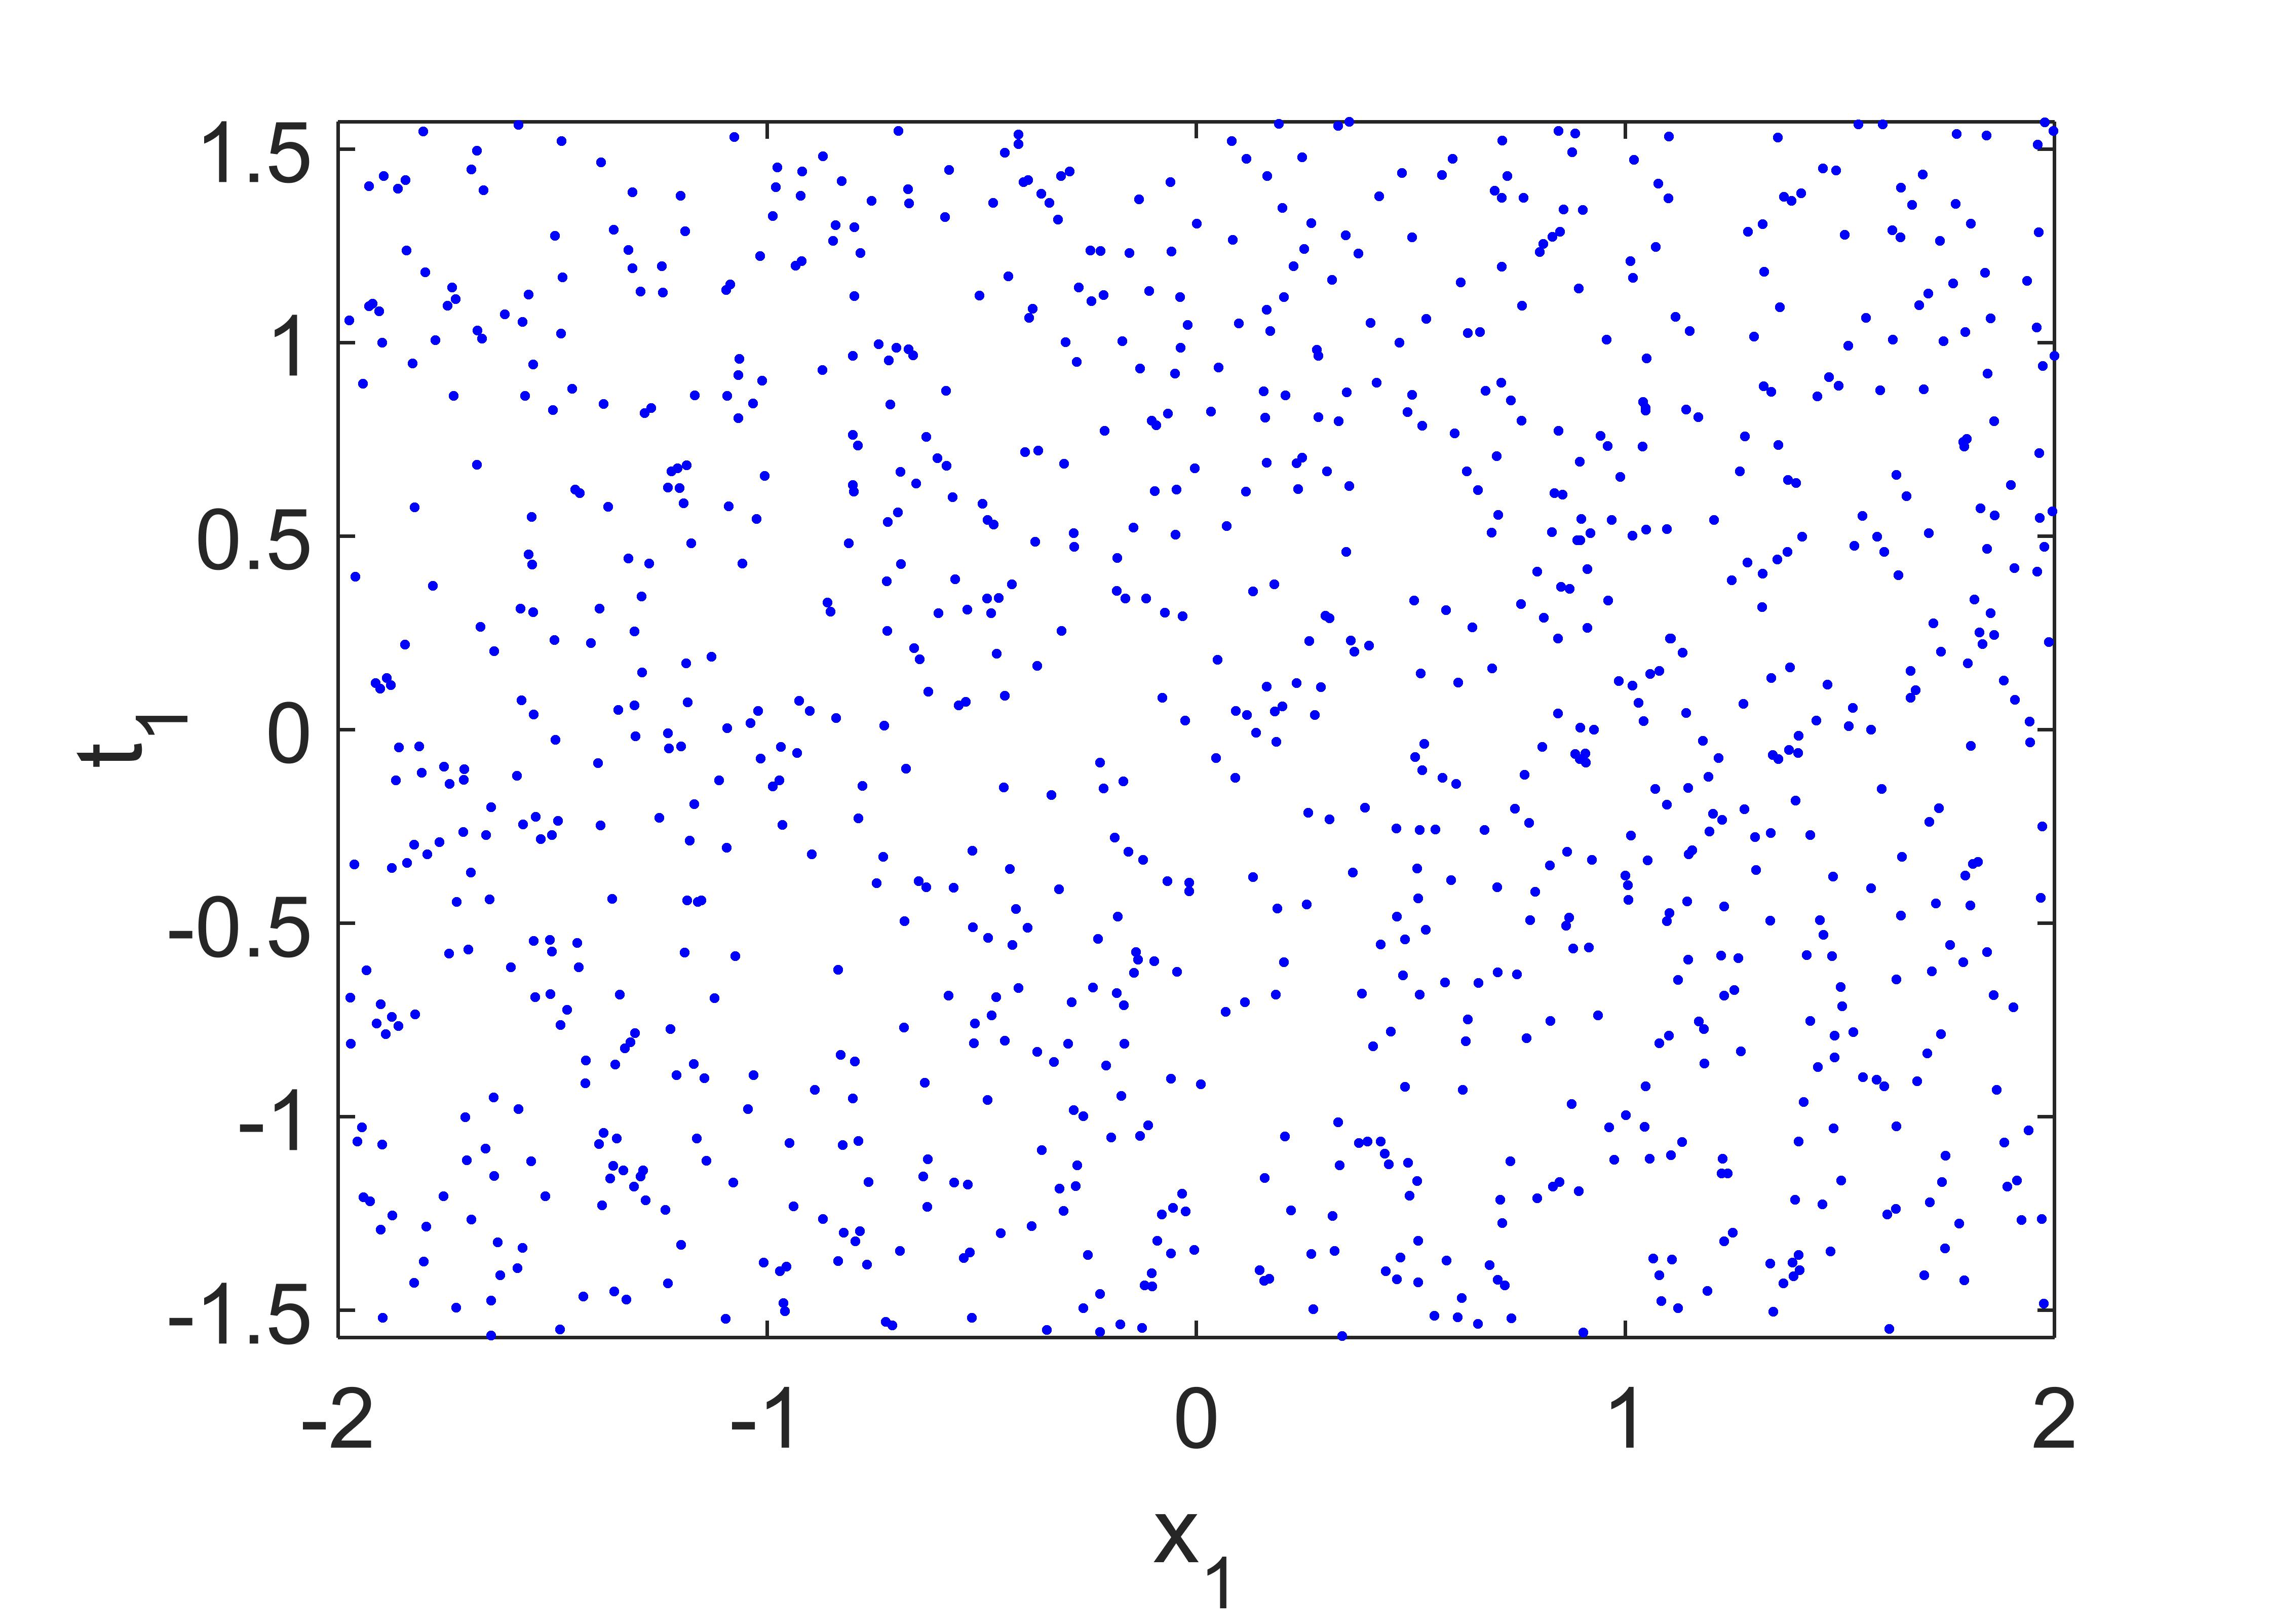
\includegraphics[width=0.8\textwidth]{mc_sample.jpg}
    \caption{Rays at the source of the two-faceted cup with random position coordinate $\variabile{x}$ and random angular coordinates $\optangle$. $10^3$ rays are depicted in this figure.}
    \label{fig:mc_sample1}
\end{center}
  \end{figure}
\\ \indent For the intensity computation we consider a sample of $10^4$ random rays and we divide the target target $\point{T} = [-\variabile{b}, \variabile{b}]$ into $\nbin= 100$ bins.
The profile of $\hat{I}_{\const{MC}}$ is depicted in Figure \ref{fig:mc_intensity} with the red line. The exact intensity is shown with the green line in the same figure.
\begin{figure}[t]
\begin{center}
    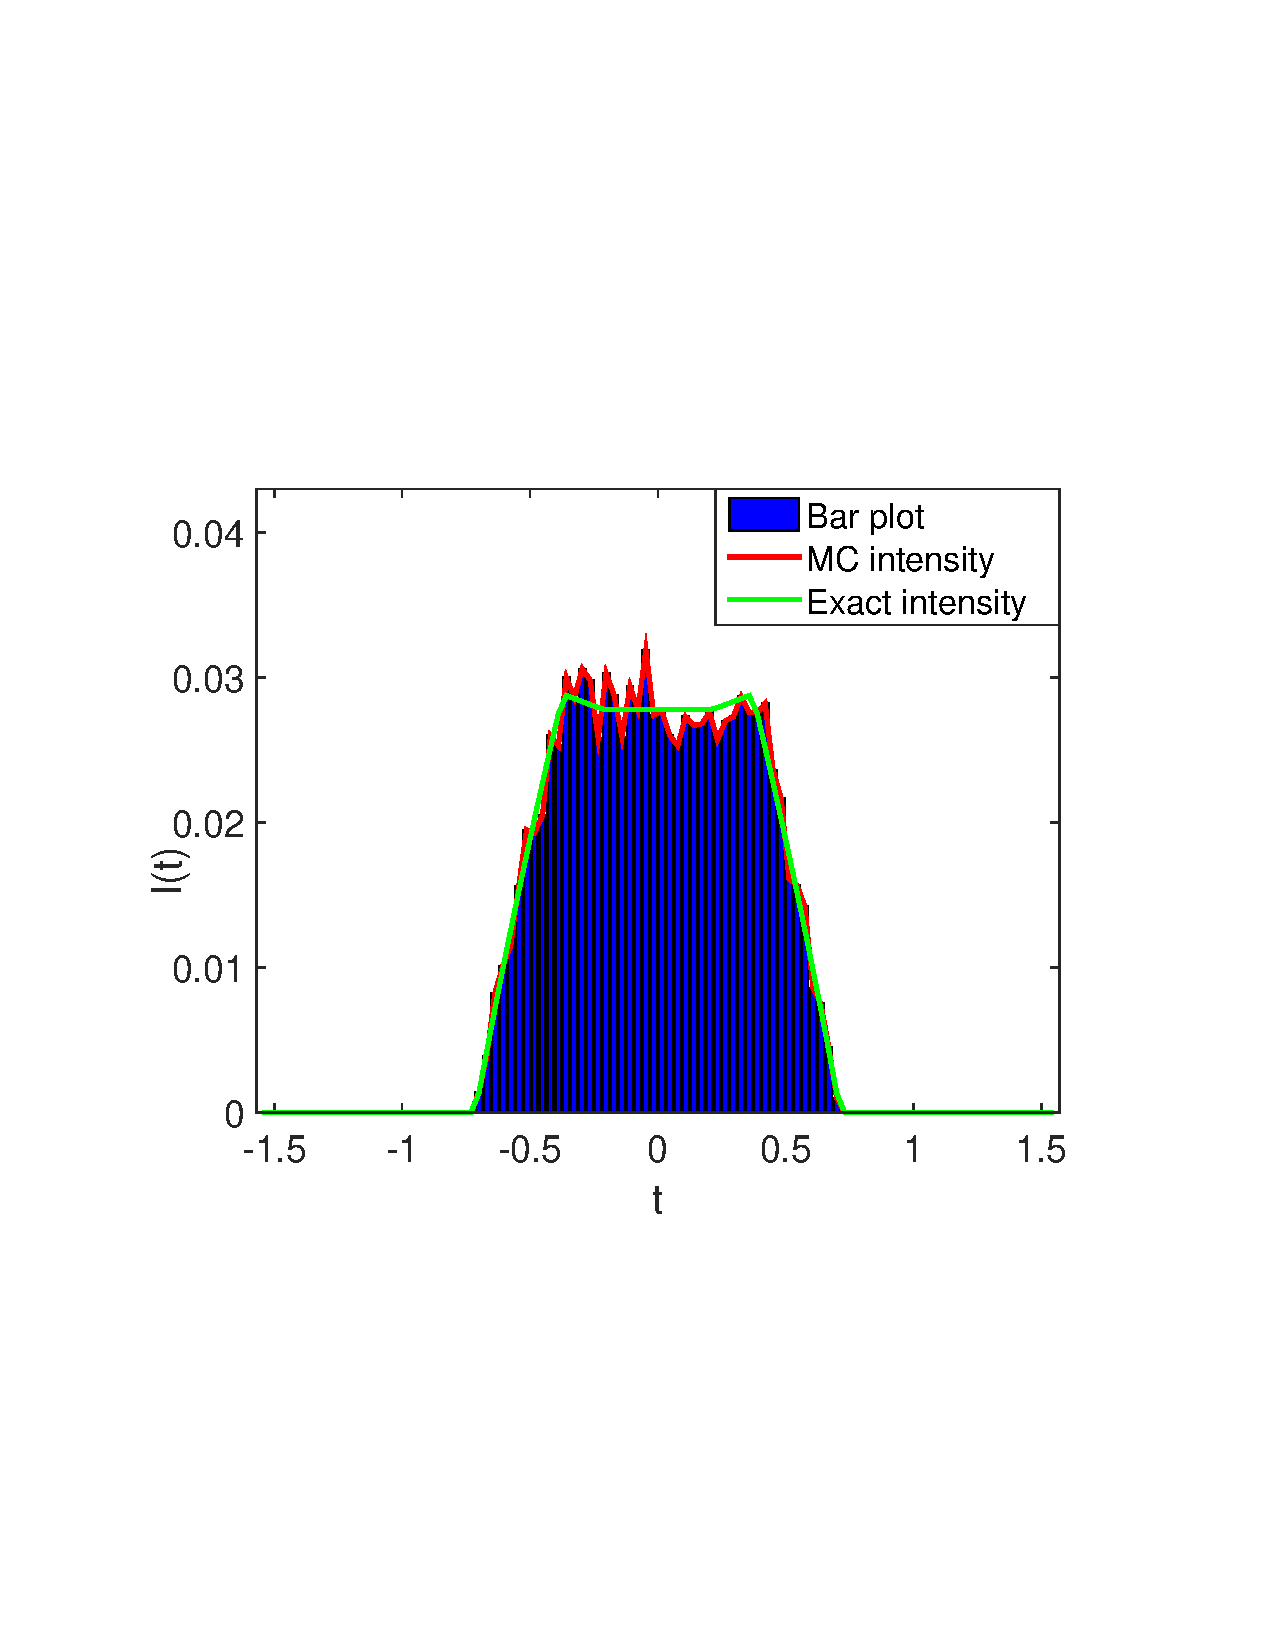
\includegraphics[width=0.8\textwidth]{MC_raytracing.jpg}
    \caption{Comparison between the averaged normalized MC intensity and the normalized exact intensity. The MC intensity is using MC ray tracing with $\nrays = 10^4$ and $\nbin = 100$.}
   \label{fig:mc_intensity}
\end{center}
\end{figure}
MC ray tracing has the advantages of being very easy to implement and it does not require too much regularity of the function that has to be approximated. Furthermore, the error convergence does not depend on the dimension of the domain in which the function is defined.
On the other hand, the MC method is time consuming as the error has a speed of convergence of order $\mathcal{O}(1/\sqrt{\nrays})$ for a large number of rays and a fixed number of bins. 
Thus, to decrease the error of a factor $10$ we need to increase the number of rays by a factor $100$.
Since MC ray tracing is a binning procedure, the error depends also on the number of bins in which the target is divided. Finally we remark that the error bound is only a \emph{probabilistic} error as shown in equation (\ref{eq:mean_error}). This means that, to calculate the value of the error, several simulations have to be repeated and the average of the errors obtained in every simulation has to be calculated. \\ \indent 
The MC noise can be reduced considering a different distribution of the initial rays set.
Instead of considering random variables, the sample of rays can be defined such that they are regularly distributed on the domain $\mbox{\insieme{D}}\subseteq\mathbb{R}^2$ of $f$. Methods based on this deterministic approach are called Quasi-Monte Carlo (QMC) methods. The ray tracing procedure that considers such rays distribution is called QMC ray tracing.
\section{Quasi-Monte Carlo ray tracing}\label{sec:QMC}
As in the previous section we first introduce QMC methods and then we briefly explain QMC ray tracing. QMC methods were proposed for the first time in the 1950s in order to speed up MC. Like MC methods, QMC procedures can be used to approximate the integral of a function $f$ using the approximation in (\ref{eq:approx_MC_QMC}).\\ \indent
This section provides basic the notions about uniform distribution theory following the Chapter $2$ of \cite{leobacher2014introduction}. 
We restrict ourselves to sets of the form $$[\vect{a}, \vect{b})= [a_1,b_1)\times[a_2, b_2)\subseteq[0,1)^2$$ and introduce the concept of sequences uniformly distributed modulo $1$.
\begin{definition}
An infinite sequence $\{\vect{y}_\variabile{n}\}_{\variabile{n}\in\mathbb{N}_0} \in [0,1)^2$ is said to be \textit{uniformly distributed modulo $1$} (or equidistributed), if for every subset $[\vect{a},\vect{b})\subseteq[0,1)^2$
\begin{equation}
\lim_{N\rightarrow \infty}\frac{\textrm{card}(\mbox{\insieme{A}}([\vect{a},\vect{b}), N))}{N} = \lambda([\vect{a},\vect{b}))
\end{equation}
where $\textrm{card}(\insieme{A}([\vect{a},\vect{b}), N))$ is the cardinality of the following set
\begin{equation}
\mbox{\insieme{A}}([\vect{a},\vect{b}), N) = \{\variabile{n}\in \mathbb{N}_0 | 0\leq\variabile{n}\leq \const{N}-1 \mbox{ and } \vect{y}_{\variabile{n}}\in [\vect{a},\vect{b})\}\,,
\end{equation} 
that is the number of $\vect{y}_{\variabile{n}}$ such that $\vect{y}_{\variabile{n}}\in [\vect{a},\vect{b})$ and $\lambda([\vect{a},\vect{b})) =(b_1-a_1)\times (b_2-a_2)$.
\end{definition}
Given a sequence $\{\vect{y}_\variabile{i}\}_{\variabile{i} = 1, \cdots, N}\in[0,1)^2$ uniformly distributed modulo $1$ and a 
Riemann integrable function $f:[0,1]^2\rightarrow \mathbb{R}$, the integral of $f$ can be approximated as the average of the values that $f$ assumes on $\{\vect{y}_\variabile{i}\}$ for every $\lineai=\{1, \cdots, N\}$, that is:
\begin{equation}
 \lim_{N\rightarrow \infty}\frac{1}{N}\sum_{\variabile{i}=1}^{N}f(\variabile{y}_{\variabile{i}}) = \int_{[0,1]^2}f(\vect{y})\textrm{d}\vect{y}.
\end{equation}
The idea of QMC methods is to generate the set of points $\vect{y}_{\variabile{i}}$ in $[\vect{a},\vect{b})$ such that they are not randomly distributed but also not exactly uniformly distributed. 
To measure how much the distribution of these points differs from a uniform distribution, the concept of discrepancy was introduced.  
Random sequences have a very high discrepancy, while uniformly distributed sequences have zero discrepancy. 
\textit{Low-discrepancy sequences} are sequences with a low discrepancy \cite{owen2003quasi} where a discrepancy of a sequence is \textit{low} if the portion of points of the sequences belonging to an arbitrary set is close to the measure of that set.
The definition of discrepancy in more mathematical terms is provided next. 
\begin{definition}
Given a set $\mbox{\insieme{Y}} = \{\vect{y}_1, \cdots, \vect{y}_N\}$ of $N$ points in $[0,1)^2$. The discrepancy $D_N(\mbox{\insieme{Y}})$ of $\mbox{\insieme{Y}}$ is defined as
\begin{equation}
D_N(\mbox{\insieme{Y}}) = \sup_{\vect{a}, \vect{b}\in[0,1)^2}\Big|\frac{\textrm{card}(\mbox{\insieme{A}}([\vect{a},\vect{b}), N))}{N}-\lambda([\vect{a}, \vect{b}))\Big|
\end{equation}
\end{definition} 
Often, it is enough to consider the discrepancy in the subset $[\vect{a},\vect{b})\subseteq[0,1)^2$ with $\vect{a}=0$, in which case we talk about star discrepancy.
 \begin{definition}
Let $\mbox{\insieme{Y}} = \{\vect{y}_1, \cdots, \vect{y}_N\}$ be a set of $N$ points in $[0,1)^2$. The  star discrepancy $D^*_N(\mbox{\insieme{Y}})$ of $\mbox{\insieme{Y}}$ is defined as:
\begin{equation}
D^*_N(\mbox{\insieme{Y}}) = \sup_{\vect{b}\in[0,1)^2}\Big|\frac{\textrm{card}(\mbox{\insieme{A}}([0,\vect{b}), N))}{N}-\lambda([0, \vect{b}))\Big|.
\end{equation}
where $\lambda([0, \point{b})) = \variabile{b}_1\;\variabile{b}_2$. 
%For intervals of the form $[\point{a}, \point{b})\subseteq [0.1)^d$ we have $\lambda_d([\point{a}, \point{b}))=\prod_{\variabile{j}=1}^{d}(\point{b}_\variabile{j}-\point{a}_\variabile{j})$.
\end{definition}
% Maybe add a picture
%Sequences constructed such that the corresponding star discrepancy is of the order of $\mathcal{O}(\log(N)^2/N)$ for $N\rightarrow\infty$ are called \textit{low-discrepancy sequences}, \cite{owen2003quasi}.
An important result shows that, using a low-discrepancy sequence $\{\vect{y}_{\variabile{i}}\}_{\variabile{i}=1, \cdots, N}$, the absolute error of a QMC algorithm in two dimensions:
\begin{equation}
\const{err}(f, S_{N}) =\Bigg|\int_{[0,1)^2}f(\vect{y}) \textrm{d}\vect{y}-\frac{1}{N}\sum_{\variabile{i}=1}^{N}f(\vect{y}_\variabile{i})\Bigg|
\end{equation}
 can be bounded by the product of a term that depends on $f$ and another term that depends on the discrepancy of the set $\{\vect{y}_{\variabile{i}}\}_{\variabile{i}=1, \cdots, N}.$ This is the result provided by the Koksma-Hlawka inequality which gives the following estimation of the error:
\begin{equation}\label{eq:QMC_error}
|\const{err}(f, S_{N})|= \Bigg|\int_{[0,1)^2}f(\vect{y}) \textrm{d}\vect{y}-\frac{1}{N}\sum_{\variabile{i}=1}^{N}f(\vect{y}_\variabile{i})\Bigg|\leq V(f)D^*_N(\mbox{\insieme{Y}}),
\end{equation}
% Explain better the variation function owen2005multidimensional
where $V(f)$ is the so-called variation function of $f$ in the sense of Hardy-Krause (see \cite{brandolini2013koksma} for details). 
The previous equation shows that for a function $f$ with finite variation $V(f)$, QMC methods perform much better than MC. However, equation (\ref{eq:QMC_error}) is not good for predicting when this will happen because $V(f)$ is hard to estimate and in some cases is infinite \cite{wang2008low}. 
%Schlier [32] reports that even for QMC the variance of f is more strongly related to the error than is the variation.
For the functions we analyze in this thesis the corresponding variation function is always bounded. 
Therefore, the convergence of QMC methods strongly depends on the low-discrepancy sequence that is used.\\ \indent
There are many ways to generate low-discrepancy sequences \cite{dalal2008low}. The most common QMC approach uses the so-called Sobol sequence. The algorithm for generating Sobol sequences is widely explained in the literature, (see for instance \cite{bratley1988algorithm}). In appendix \ref{app:Sobol} we give an overview of how these kind of sequences can be constructed. When using Sobol sequences QMC error can be estimated by:
\begin{equation}
\const{err}(f, S_{N})<\const{C} \frac{\log(N)^2}{N}, 
\end{equation}
for some $\const{C}>0$.
For higher dimensions $d>2$, the general relation holds
\begin{equation}
\const{err}(f, S_N)<\const{C} \frac{\log(N)^d}{N}.
\end{equation}
%For small dimensions, QMC performs much better than MC methods, while for large dimension the factor $\log(\const{N})$ could be very big. 
% In the following we show a particular construction of a low-discrepancy sequence for $d=1$ that was introduced the first time by Van der Corput in 1935.  
%This kind of sequences, called \textit{van der Corput} sequences, are particular interesting not only because they give an intuition of how to construct low discrepancy sequences but also because many other kind of sequences in higher dimensions are based on this one-dimensional case. Before introducing these sequences we need to give the concept of radical inverse function. Let $\const{b}\geq 2$ be an integer base. Any natural number $\variabile{n}\in \mathbb{N}_0$ can be decomposed in base $\const{b}$ as follows:
%\begin{equation}
%\variabile{n} = \sum_{\variabile{i}=0}^\infty \variabile{d}_{\variabile{i}}\const{b}^{\variabile{i}}
%\end{equation}
%where $\variabile{d}_{\variabile{i}} \in \{0, 1, \cdots, \const{b}-1\}$ are the digit numbers.
%The radical inverse function $\phi_{\const{b}}:\mathbb{N}_0\mapsto [0,1)$ in base $\const{b}$ is defined as:
%\begin{equation}
%\phi_{\const{b}}(\variabile{n}) = \sum_{\variabile{i}=1}^{\infty}\frac{\variabile{d}_{\variabile{i}-1}}{\const{b}^{\variabile{i}}}.
%\end{equation}
%As an example we provide in the following the radical inverse function $\phi_{\const{b}}(5)$ in base $\const{b} = 2$. 
%The digit expansion in base $\const{b}$ of $\variabile{n}=5$ is:
%\begin{equation}
%5 = 1\cdot 2^0+1\cdot 2^2.
%\end{equation}
%Therefore, $\variabile{d}_0 = 1, \variabile{d}_1 = 0$ and $\variabile{d}_2 = 1$. 
%The radical inverse function $\phi_2(5)$ is:
%\begin{equation}
%\phi_2 (5) = \frac{1}{2}+\frac{1}{8} = \frac{5}{8}.
%\end{equation}
%\begin{definition}
%The Van der Corput sequence in base $\const{b}$ is defined as $\{ \phi_{\const{b}}(\variabile{n})\}_{n\in\mathbb{N}_0}$.
%\end{definition}
%For example, suppose we have the finite sequence of numbers $\variabile{n}\in \{0, 1,\cdots, 8\}$  the corresponding Van der Corput sequence 
%$\{ \phi_{\const{b}}(\variabile{n})_{\variabile{n}\in \{0, 1,\cdots, 8\}}$ in base $\variabile{b}=2$ is:
%\begin{equation}
%\big\{\phi_2(\variabile{n})\big\}_{\variabile{n}\in \{0, 1,\cdots, 8\}} = \Bigg\{0, \frac{1}{2}, \frac{1}{4}, \frac{3}{4}, \frac{1}{8},\frac{5}{8}, \frac{3}{8}, \frac{7}{8}, \frac{1}{16}\Bigg\} \,.
%\end{equation}
%It can be proved that the Van der Corput sequence in base $\variabile{b}$ is uniformly distributed modulo one, \cite{leobacher2014introduction}. 
%The van der Corput sequence has been extended to higher dimensions. 
%The most common QMC approach uses Sobol sequence which is one an extended Van der Corput sequence in base $\variabile{b}=2$ to $\variabile{d}\geq2$. 
\\ \indent Ray tracing based on QMC methods considers as position and angular coordinates of the rays at the source, the coordinates of the corresponding points of a low-discrepancy sequence. 
Therefore, to implement QMC ray tracing in two-dimensions we need to construct a low-discrepancy sequence in two-dimensions.  
Given, for instance, a Sobol sequence $\{\vect{y}_{\variabile{i}}\}_{\variabile{i}=1, \cdots, N}$ with $\vect{y}_\variabile{i}\in[0,1)^2$ for every $\variabile{i}=1, \cdots, N$, the two dimensional QMC ray tracing the coordinates $(\variabile{x}_1^{\variabile{i}}, \optangle_1^{\variabile{i}})$ of the $\variabile{i}$-th ray at the source equal to those of the $\variabile{i}$-th points of the sequence, i.e., $(\variabile{x}_1^{\variabile{i}}, \optangle_1^{\variabile{i}})=\vect{y}_{\variabile{i}}$. A set of $\nrays = N$ rays with these initial coordinates is traced within the system and the target coordinates of all the rays traced are computed. \\ \indent 
Similarly to MC ray tracing, the averaged and normalized QMC intensity $\hat{I}_{\const{QMC}}$ is given by the approximation in (\ref{eq:approx_MC_QMC}), where now the variable $\vect{y}$ is a variable of the Sobol sequence instead of a random variable. Therefore, the target is divided into $\nbin$ bins and the averaged number of rays that follow into each bin is considered. The intensity is still a piecewise constant function, and its value over every bin $[\optangle_{\variabile{j}-1}, \optangle_{\variabile{j}})_{\variabile{j}=1, \cdots, \nbin}$ is given by the intensity $\hat{I}_{\textrm{QMC}}(\optangle_{\variabile{j}-1/2})$ calculated along the direction $\optangle_{\variabile{j}-1/2} = \frac{(\optangle_{\variabile{j}-1}+\optangle_{\variabile{j}})}{2}$ (middle point of the bin). The only difference between MC and QMC ray tracing consists on the choice of the initial ray set. Thus, we expect that QMC and MC errors have the same dependence on the number of bins $\nbin$. More precisely, since the discretization error (first term on the right hand side of inequality (\ref{eq:error_int})) does not depend on MC noise, we expect that it does not change for QMC error. Regarding the second terms on the right hand side of inequality (\ref{eq:error_int}), we showed in the previous section that it depends on the standard deviation of the approximated intensity and on the number of bins. Hence, indicating with $I(\optangle_{\variabile{j}-1/2})$ the exact value of the intensity at direction $\optangle_{\variabile{j}-1/2}$, we can predict that the QMC error over every bin is estimated by:
\begin{equation} \begin{aligned}
\Big|I(\optangle_{\variabile{j}-1/2})&-\frac{\Phi}
{\Delta\optangle}\hat{I}_{\const{QMC}}(\optangle_{\variabile{j}-1/2})\Big| \leq
\frac{\const{C}_1}{\nbin^2} + \const{C}_2\sqrt{\nbin}\frac{\log(\nrays)-\log(\nbin)}{\nrays},
\end{aligned}
\end{equation}
for some $\const{C}_1>0$ and $\const{C}_2>0$.
\\ \indent
In Figure \ref{fig:qmc_sample1} we show the distribution of the position and direction coordinates of the rays at the source of the two-faceted cup in Figure \ref{fig:cup}. 
A set of $10^3$ rays generated from a $2D$ Sobol sequence is considered, the coordinates $(\variabile{x}_1, \optangle_1)$ of every ray at the source are depicted with blue dots.
We note that the rays have a regular distribution on the $(\variabile{x}, \optangle)$-plane.
We need to remark that, for the system in Figure \ref{fig:cup}, $\variabile{x}_1 \in[-2,2]$ and the angular coordinates $\optangle_1 \in[-\pi/2, \pi/2]$. 
Since Sobol sequences are defined inside intervals of the  $[\vect{a}, \vect{b})\subseteq[0,1)^2$, we scaled the points of the sequence $\vect{y}_{\variabile{i}}$ in order to take all the possible positions and directions that the rays can assume at the source, therefore, for this system, $\variabile{x}_1^{\variabile{i}} = -2+4\,y_{\variabile{i}}(1)$ and $\optangle_1^{\variabile{i}} = -\pi/2+\pi\,y_{\variabile{i}}(2)$ where 
$\vect{y}_{\variabile{i}} = \big(y_{\variabile{i}}(1), y_{\variabile{i}}(2)\big)$ is a point of the Sobol sequence. 
\begin{figure}[t]
\begin{center}
    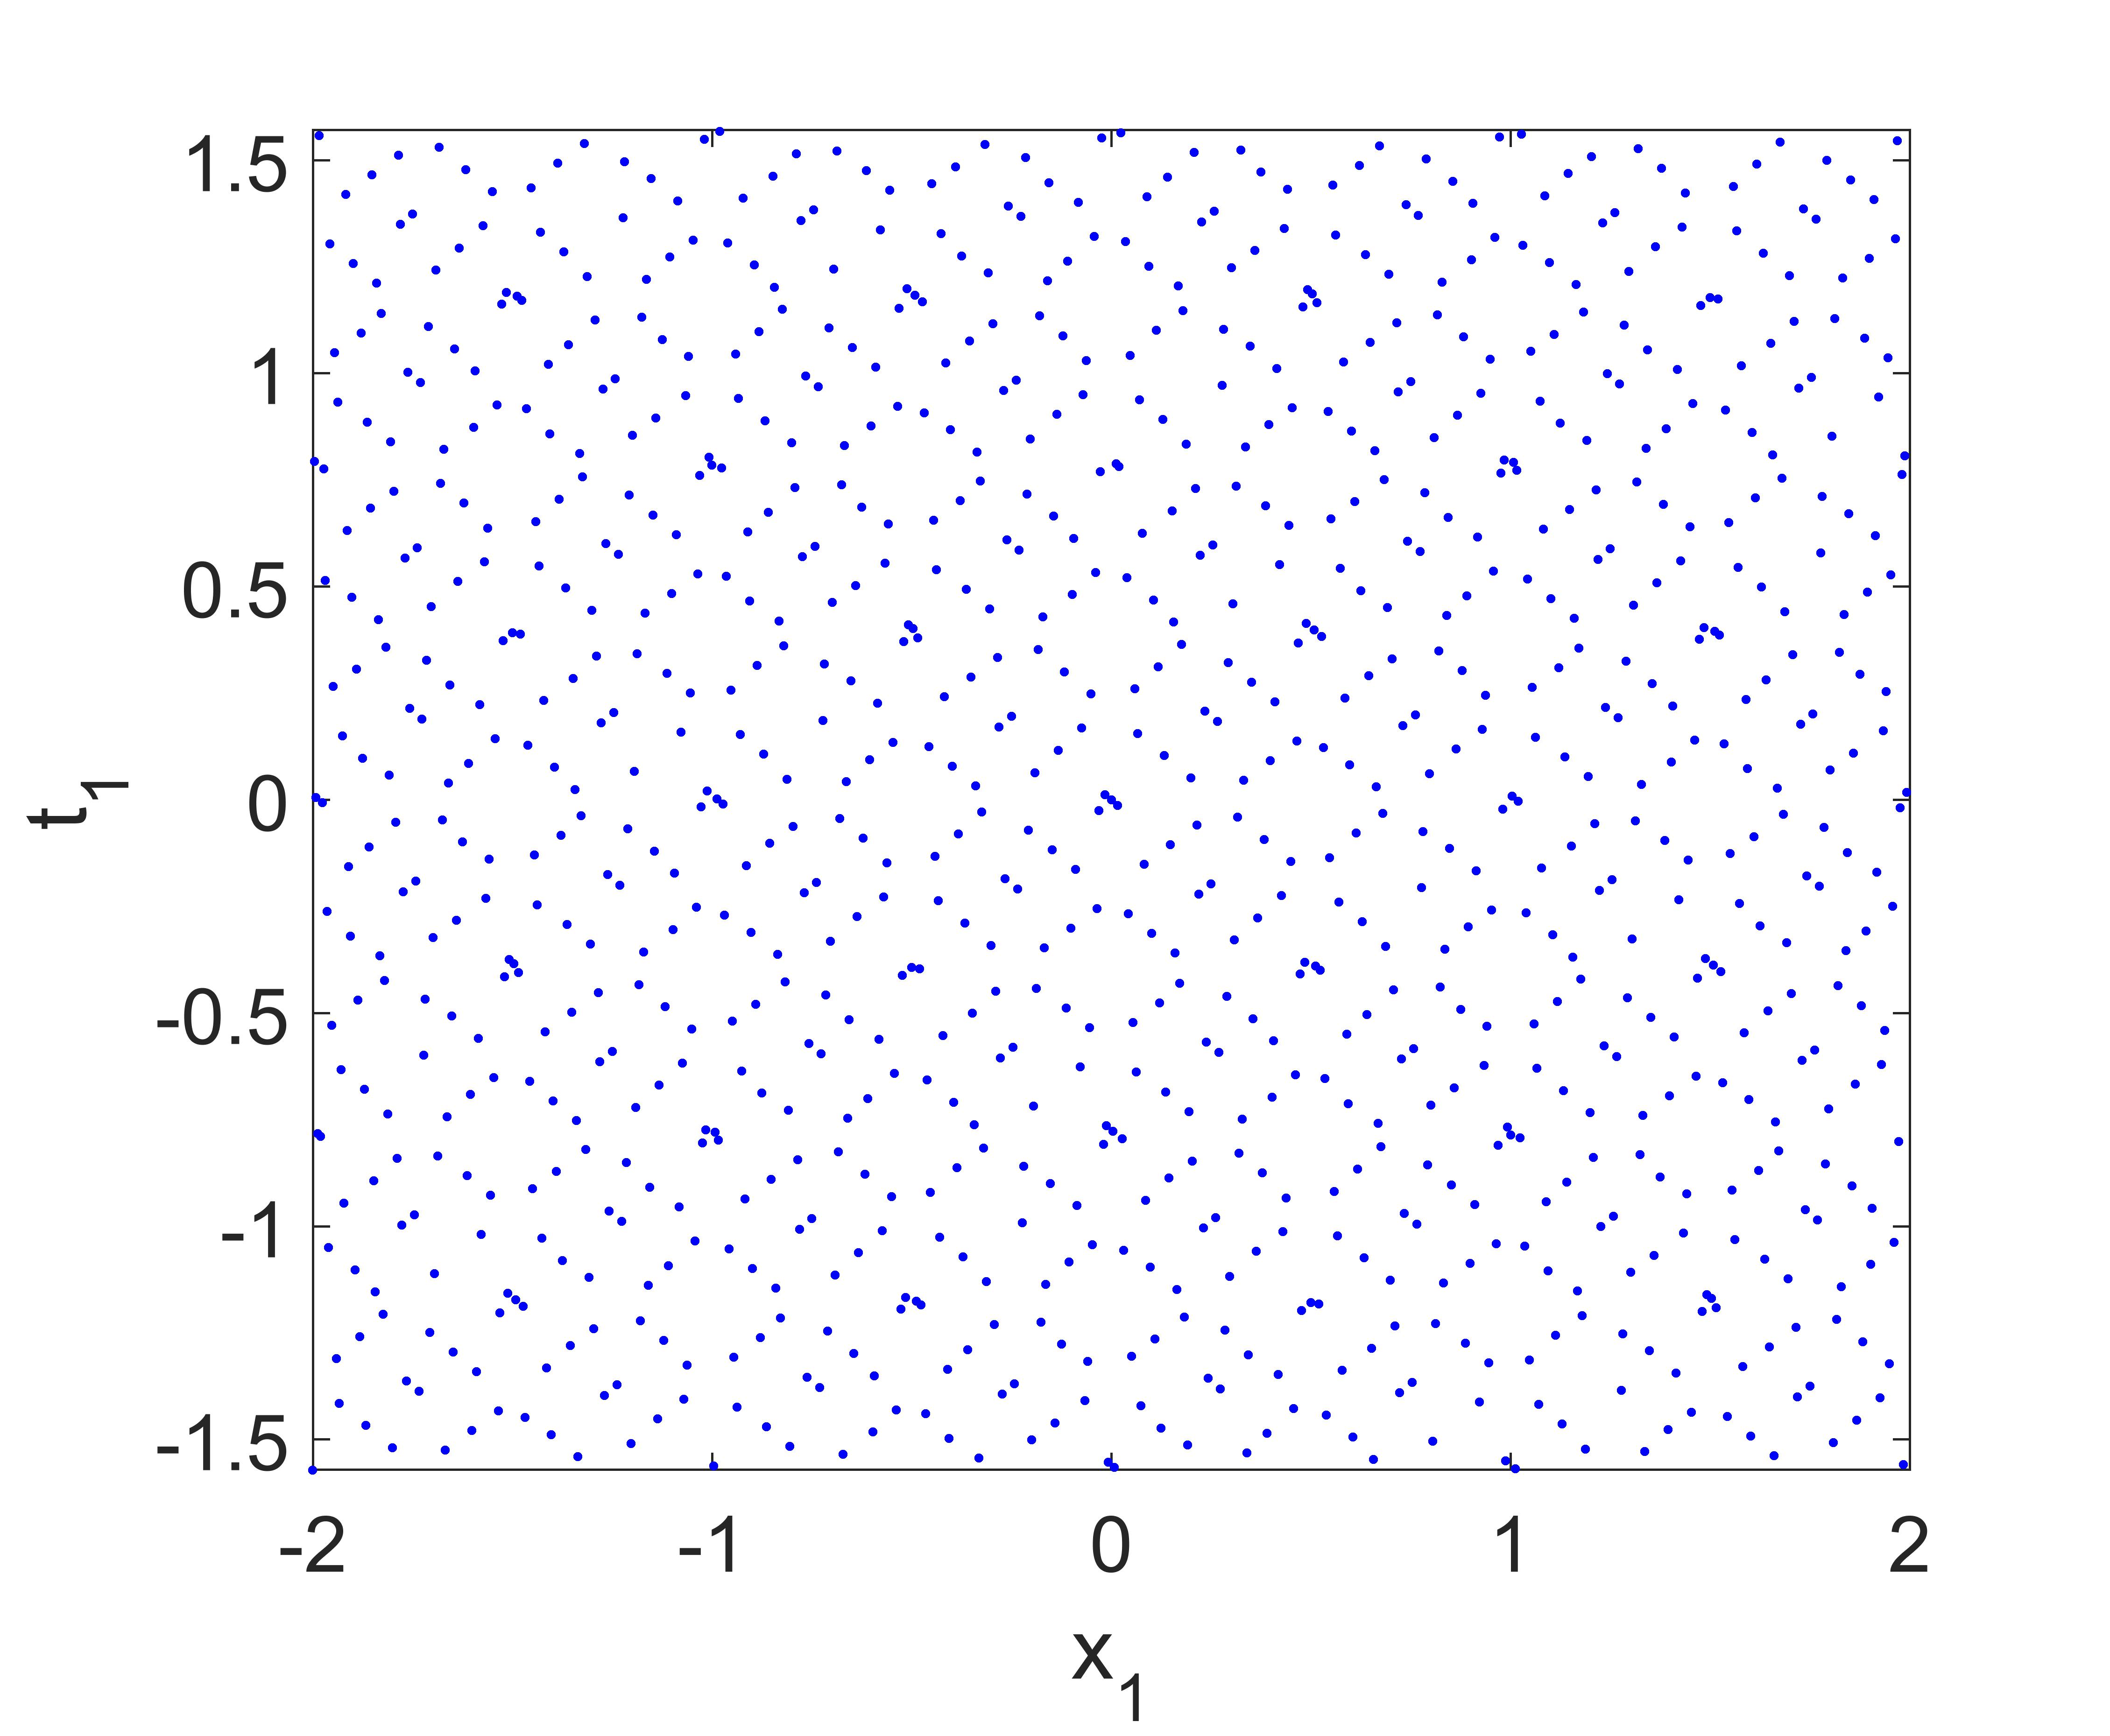
\includegraphics[width=0.8\textwidth]{qmc_sample.jpg}
    \caption{$10^3$ rays at the source of the two-faceted cup with position coordinate $\variabile{x}_1$ and angular $\optangle_1$ coordinate with a regular distributions.
They are distributed as the points of a Sobol sequence in two-dimensions.}
    \label{fig:qmc_sample1}
\end{center}
  \end{figure}
\\ \indent Dividing the target into $\nbin=100$ bins, we computed the target intensity. 
In Figure \ref{fig:qmc_intensity} we show the profile of the output intensity at the target of the two-faceted cup computed using QMC ray tracing with $10^4$ rays. 
The QMC intensity is depicted with the red line. It is compared to the exact intensity shown in the same figure with the green dotted line.
A comparison between Figure \ref{fig:mc_intensity} and \ref{fig:qmc_intensity} shows that for the two-faceted cup and for a set of $\nrays=10^4$ rays, QMC ray tracing performs better than MC ray tracing. In order compare MC and QMC ray tracing, we calculate the target intensity using both methods gradually increasing the number of rays traced inside the two-faceted cup. The errors between the approximated averaged normalized intensity $\hat{I}_{\textrm{A}} (\textrm{A} = \textrm{MC}, \textrm{QMC})$ and the exact normalized intensity $\hat{I}_\textrm{exact}$ are calculated.
% Explain the speed of convergence
The speed of convergence for MC is shown in Figure \ref{fig:Error_cup} with the red, while the behavior of QMC ray tracing is depicted in the same picture with the blue line.
The results shown for a simple optical system are indeed consistent with what we expected from the theoretical analysis.
\\\indent Although QMC ray tracing is an improvement of MC ray tracing for small dimensions, it has still two main disadvantages. 
First, its convergence is strongly related with the dimension in which it is implemented.
Second, likewise MC ray tracing, QMC ray tracing is a binning procedure, therefore the error still depends on the number of bins in which the target is divided and only the averaged value of the intensity over every bin is provided.
\begin{figure}[t]
\begin{center}
    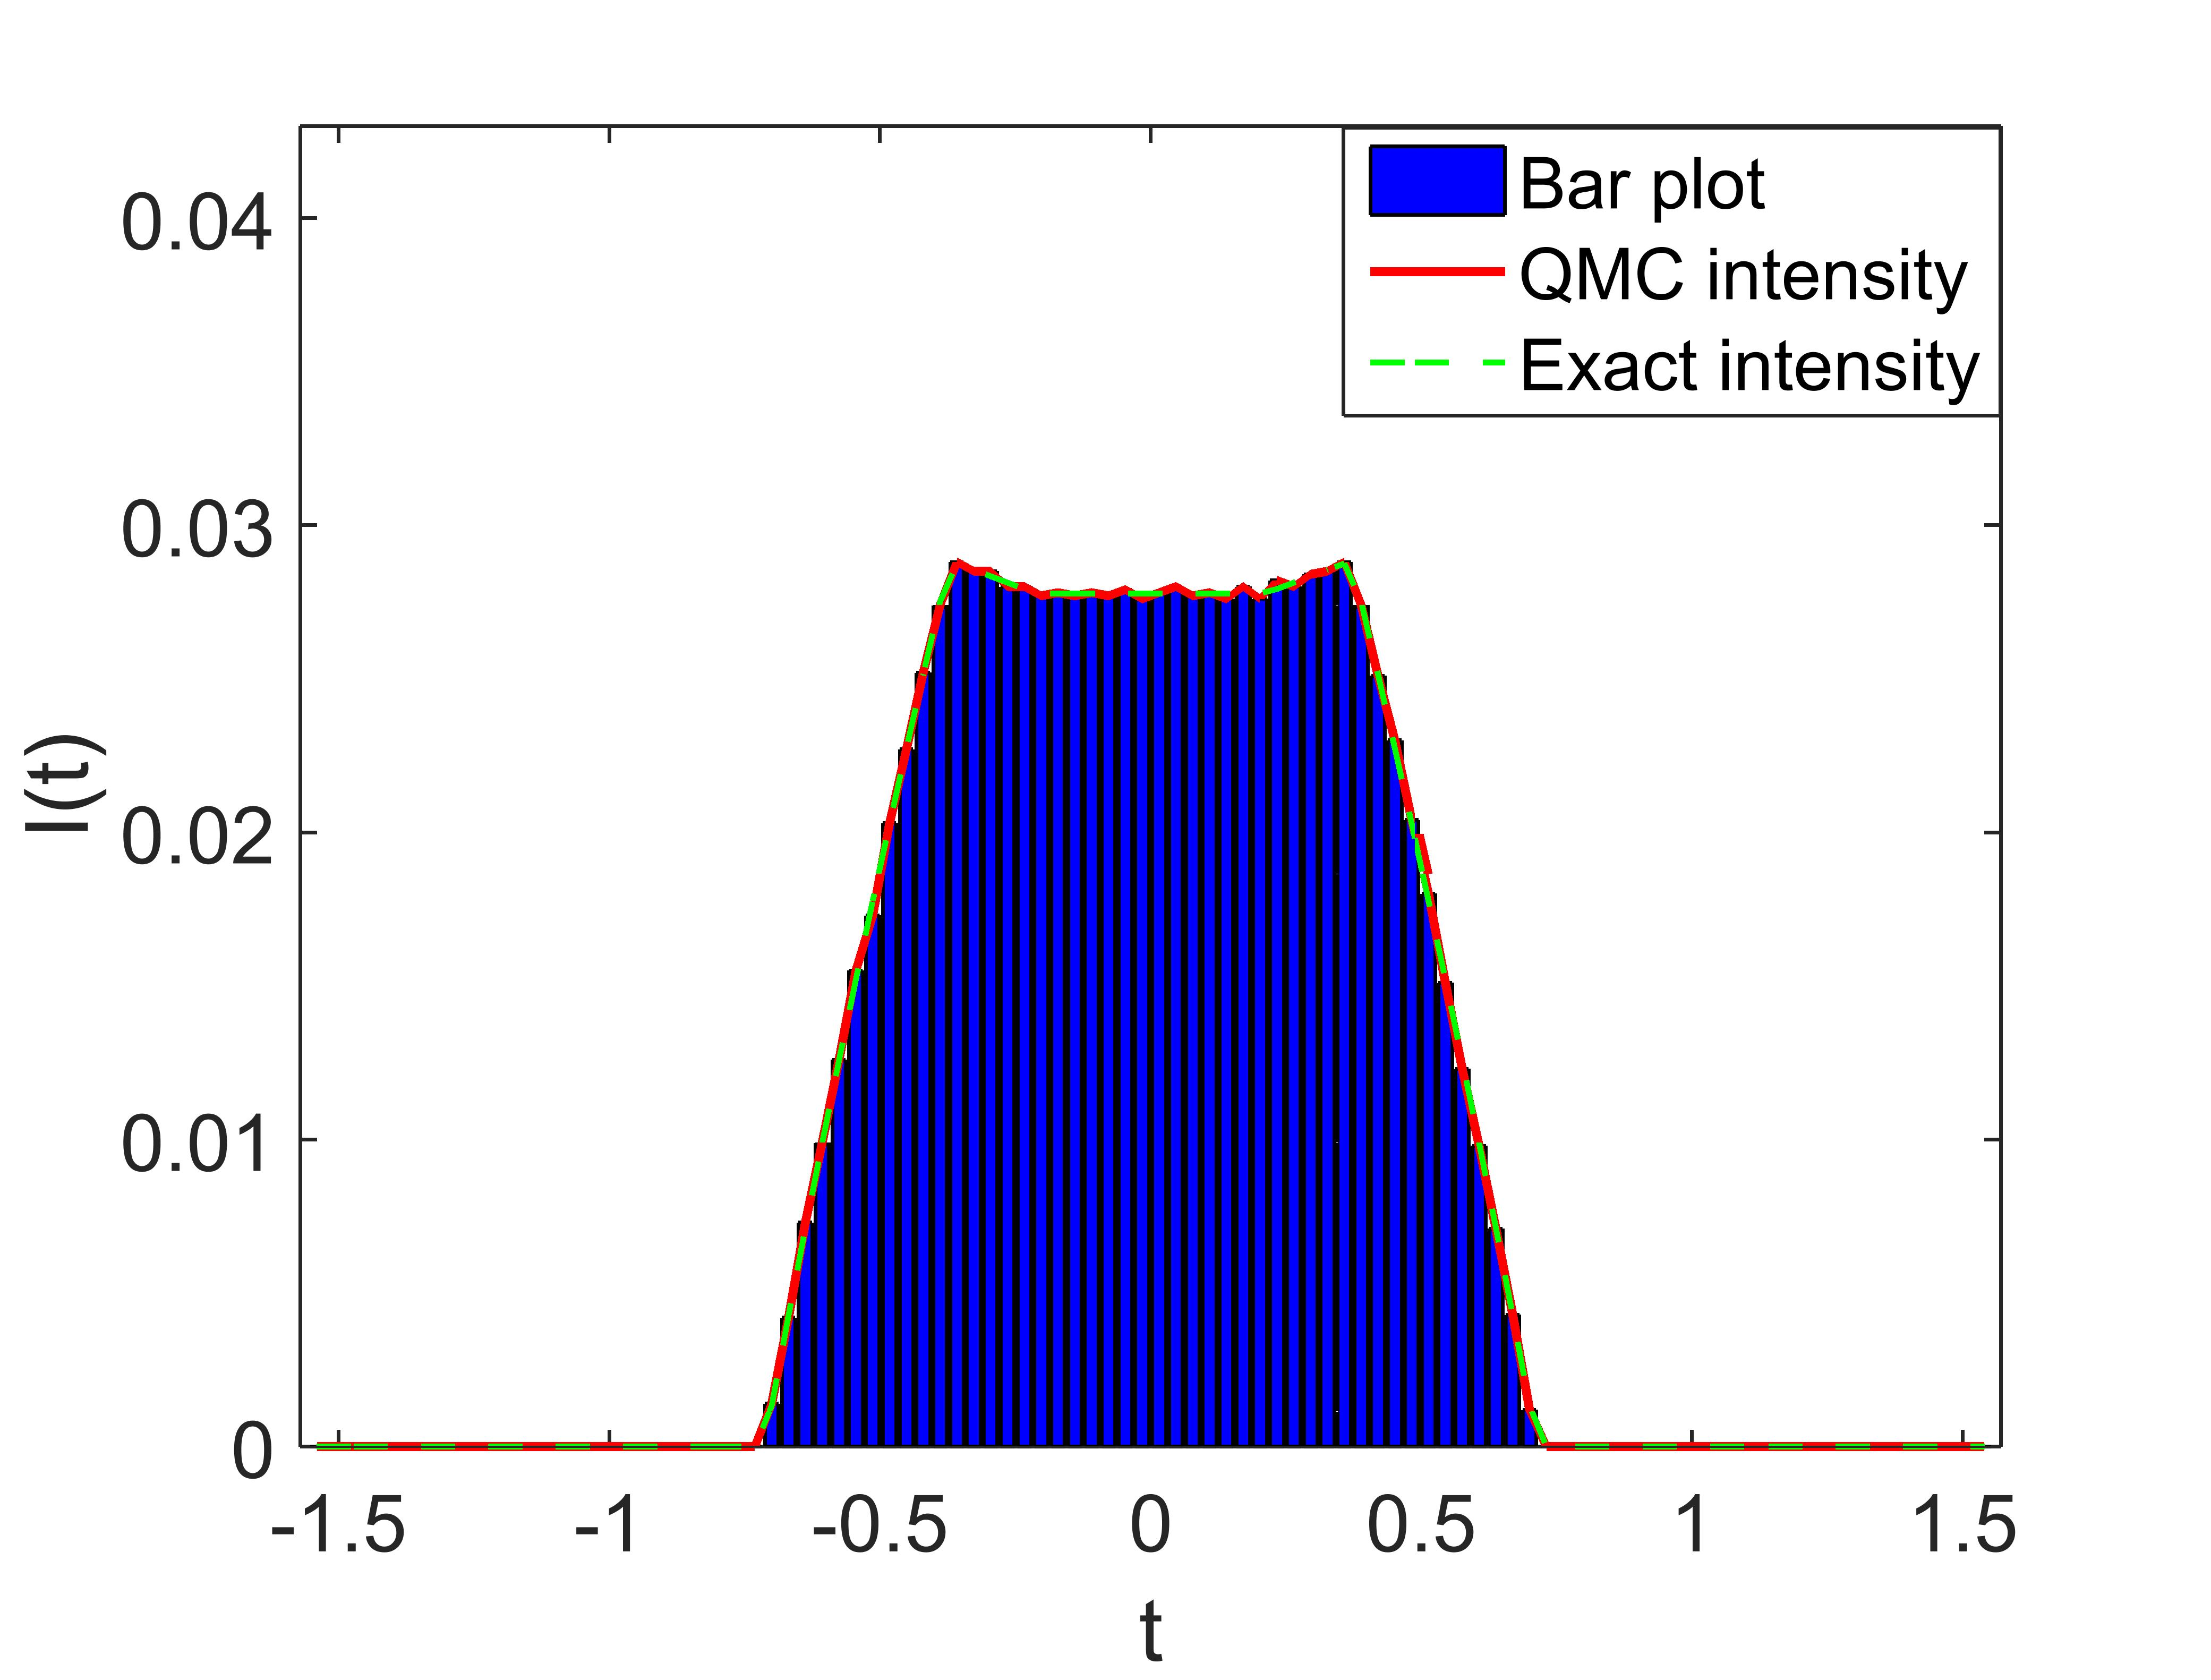
\includegraphics[width=0.8\textwidth]{qmc_raytracing.jpg}
    \caption{QMC intensity for the two-faceted cup obtained tracing $\nrays=10^4$ rays and dividing the target into $\nbin=100$ bins.}
    \label{fig:qmc_intensity}
\end{center}
  \end{figure}
\begin{figure}[h]
\begin{center}
    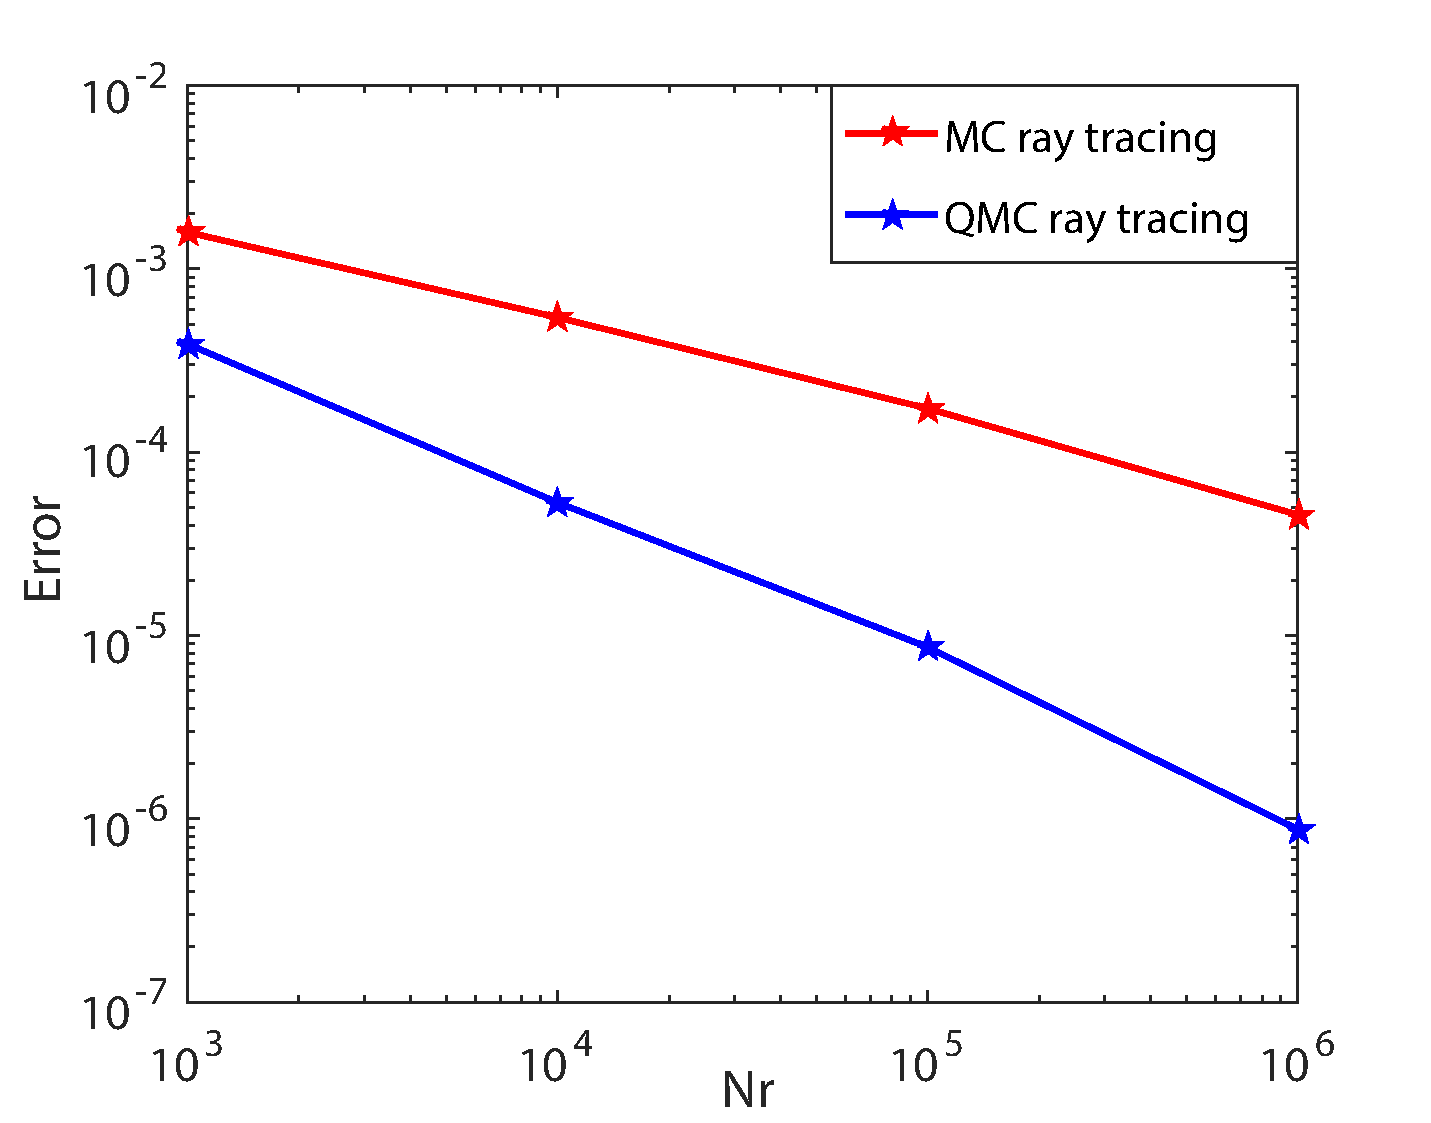
\includegraphics[width=0.8\textwidth]{Error_cup}
    \caption{Error as function of the number of rays traced in a logarithmic scale for fixed number of bins $\nbin=100$.
 MC ray tracing convergence is of the order $\mathcal{O}(1/\sqrt{\nrays})$ and it is shown with the red line. 
QMC ray tracing convergence is of the order $\mathcal{O}(1/\nrays)$ and it is depicted with the blue line.}
    \label{fig:Error_cup}
\end{center}
  \end{figure}
 \\ \indent
From the results provided in this chapter we can conclude that the choice of the initial ray set can make a big impact on the performance of the ray tracing procedure. 
Based on the idea of taking a smart choice of the initial ray set, we develop a new ray tracing method which is based on phase space. 
The phase space (PS) concept will be introduced in the next chapter. The new ray tracing method employs the PS of the source and the target of the optical systems.
We will show that phase space ray tracing allows to trace a relatively small number of rays inside the system to obtain the desired accuracy of the target intensity. 






















\chapter{Ray tracing on phase space} \label{chap:PS}
Ray tracing on phase space is a method which employs the phase space (PS) of the source and the target of the optical system.
Moreover, it takes into account the trajectory that every ray follows during its propagation.
Before explaining the method, we introduce the PS concept.
\section{Phase space}\label{sec:PSconcept}
Every ray in three dimensions can be described by three position coordinates and three direction coordinates. 
The PS of an optical surface is a four-dimensional space characterized by two position and two direction coordinates. The position coordinates are two of the coordinates of the intersection point of the ray with the surface, while the direction coordinates are the momentum coordinates of the vector tangent to the ray projected on that optical surface \cite{wolf2004geometric}.
\\ \indent 
In two dimensions, every ray parametrization is obtained from two position and two direction coordinates. The PS of an optical line is described by one position and one direction coordinate. Hence, for two-dimensional systems, every ray in PS is described by a point in a two-dimensional space.
Given an optical line $\lineai$, the ray position coordinate on PS is the $\variabile{x}$-coordinate of the intersection point between the ray and the line $\lineai$. The direction coordinate is the sine of the angle that the ray forms with respect to the normal \vect{$\boldsymbol{\nu}$} of line $\lineai$ multiplied by the index of refraction \n. We choose \vect{$\boldsymbol{\nu}$} always directed inside the same medium in which the incident ray travels. The PS is indicated with \set{S}{}{}$=$\set{Q}{}{}$\times$\set{P}{}{},
where \set{Q}{}{} is the set of the position coordinates \variabile{q} and \set{P}{}{} is the set of the direction coordinates $\variabile{p}=\variabile{n}\sin{\myangle}$, with $\myangle\in[-\pi/2, \pi/2]$ the angle between the ray segment inside the system and the normal measured counterclockwise.
In the following, the PS is considered only for the source $\point{S}$ and the target $\point{T}$ and for no other line of the optical system.
The coordinates of every ray on \set{S}{}{} and \set{T}{}{} are indicated with $(\variabile{q}_1,\variabile{p}_1)$ and $(\variabile{q},\variabile{p})$, respectively.\\ \indent
\begin{figure}[t]
  \begin{minipage}[]{0.49\textwidth}
\centering
    \includegraphics[width  = \textwidth]{source_PS_cup1_rev.pdf}
    \caption{\textbf{Source PS.} Five different paths can occur for the two-faceted cup.}
    \label{fig:sourcePS1}
  \end{minipage}
\hfill
  \begin{minipage}[]{0.49\textwidth}
\centering
    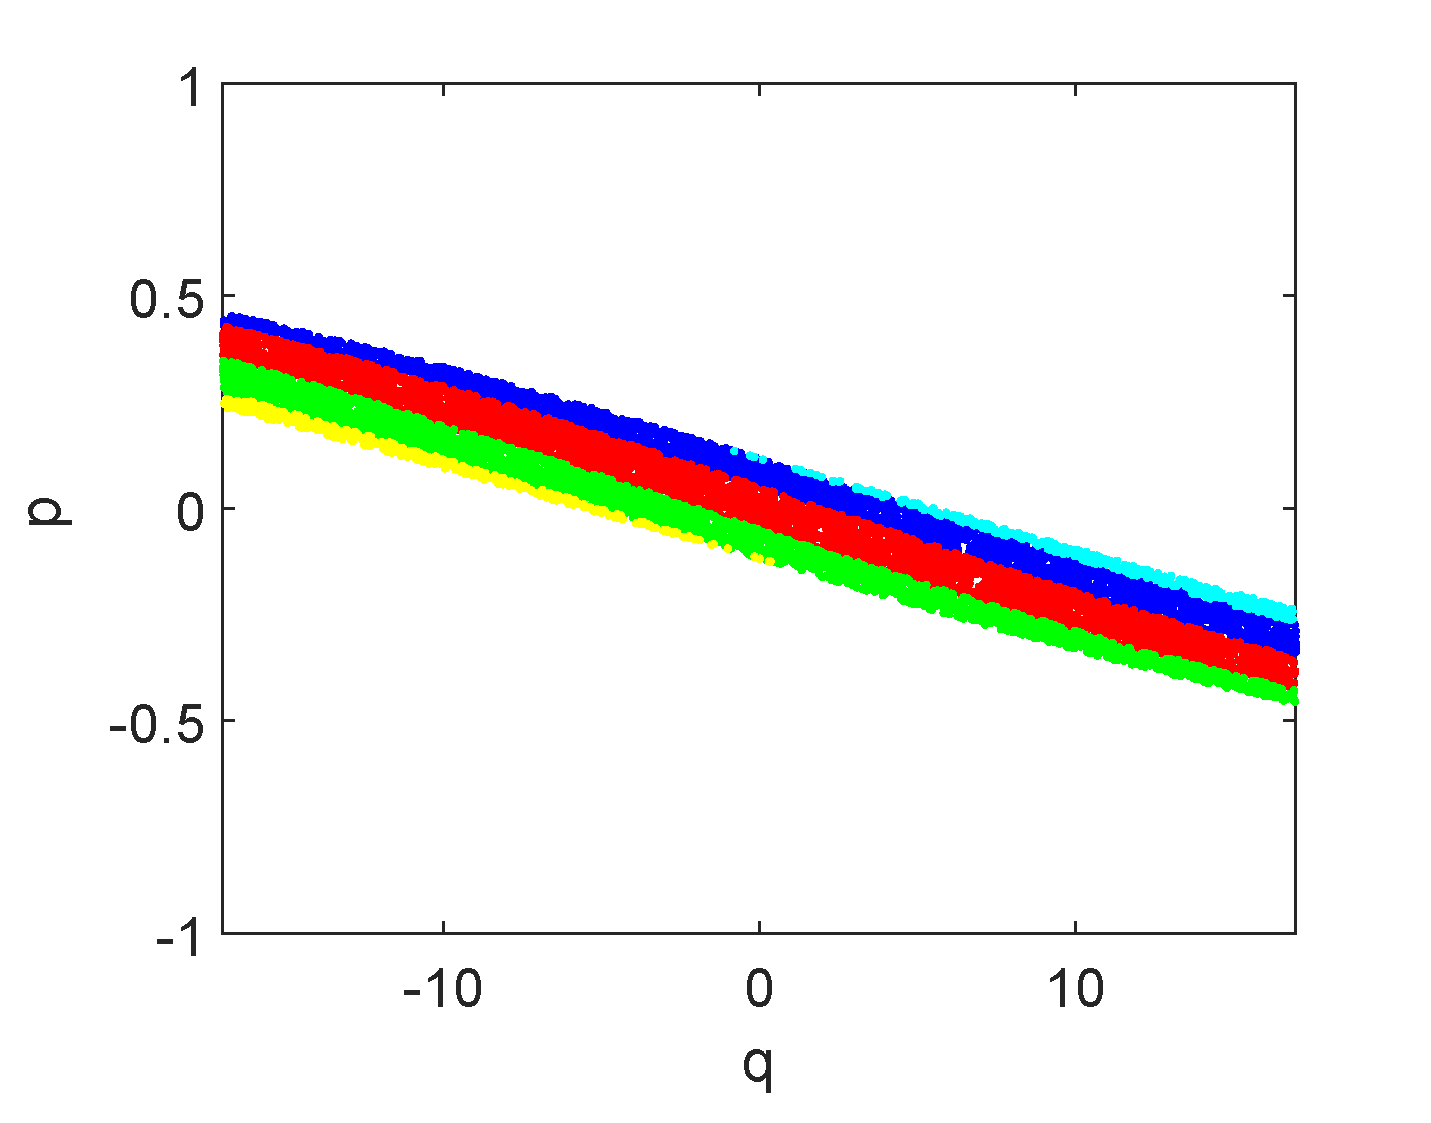
\includegraphics[width=\textwidth]{target_PS_cup.pdf}
  \caption{\textbf{Target PS.} Five different paths can occur for the two-faceted cup.}
   \label{fig:targetPS1}
 \end{minipage}
\end{figure}
As an example, in Figures \ref{fig:sourcePS1} and \ref{fig:targetPS1} we show the source and target PS of the two-faceted cup (in Figure \ref{fig:cup}), sampled with $10^4$ random rays. The coordinates of every point correspond to the position and direction coordinates of a ray which are calculated using the ray tracing procedure. Furthermore, we store the path $\Pi$ that every ray follows, where we refer to a path as the sequence of lines encountered by the ray.
In Figures \ref{fig:sourcePS1} and \ref{fig:targetPS1} a color is associated to every path.
We note that the source and target phase spaces are partitioned into different regions according to the path $\Pi$ followed by the rays.
Given a path $\Pi$, the corresponding regions are indicated with $\mbox{\insieme{R}}_\textrm{s}(\Pi)$ and $\mbox{\insieme{R}}_\textrm{t}(\Pi)$ at source and target PS, respectively.
Rays that propagate through the two-faceted cup can follow $5$ different paths. Some rays are emitted from the source and arrive at the target without hitting any other line, they follow path $\Pi_1= (1,4)$. These rays are depicted in red in the PS pictures. Some other rays can hit the left or the right reflector (line $2$ and $3$, respectively) once, their corresponding paths are $\Pi_2 = (1,2,4)$ and $\Pi_3 = (1,3,4)$, respectively. These rays are the green and blue dots in PS. Finally, there is the possibility that the rays have two reflections before hitting the target. They follow either path $\Pi_4 = (1,2,3,4)$ or path $\Pi_5 = (1,3,2,4)$ and they are depicted with the cyan and yellow points.
\\ \indent For the two-faceted cup all light emitted by the source arrives at the target. In order to derive the photometric variables at the target we need to understand where light ends up, i.e., which parts of the target PS are illuminated by the source. Indeed, while the source PS is completely covered by rays, some parts of the target PS are not reached by any ray at all.
%, that is 
%\begin{equation}
%\begin{aligned}
%\mbox{\insieme{S}} &= \bigcup_{\Pi} \mbox{\insieme{R}}_\textrm{s}(\Pi),\\
%\mbox{\insieme{T}} &\supset \bigcup_{\Pi} \mbox{\insieme{R}}_\textrm{t}(\Pi),
%\end{aligned}
%\end{equation}
%where the unions are over all the possible paths.
This means that, while the luminance at the source PS is positive for any possible position and direction, the luminance at the target PS is positive only inside the regions $\mbox{\insieme{R}}_\textrm{t}(\Pi)$, for every path $\Pi$, and it is equal to $0$ outside those regions. For this reason, from now on we will refer to $\mbox{\insieme{R}}_\textrm{t}(\Pi)$ as the \textit{positive luminance regions}. \\ \indent
It is very important to remark that, although \insieme{S} and \insieme{T} have a different ray distribution, the area covered by the rays is conserved. This follows from \'{e}tendue conservation. From (\ref{etendue2d}) we rewrite the two-dimensional \'{e}tendue as:
\begin{equation}
U = \int_{\variabile{x}^{\textrm{min}}}^{\variabile{x}^{\textrm{max}}} \int_{\myangle^{\textrm{min}}}^{\myangle^{\textrm{max}}} \n \cos(\myangle)\textrm{d}\variabile{x}\,\textrm{d}\myangle= \int_{\mbox{\set{P}{}{}}}\int_{\mbox{\set{Q}{}{}}} \textrm{d}\variabile{q}\,\textrm{d}\variabile{p}.
\end{equation}
where we indicated with $\variabile{x}^{\textrm{min}}$ and $\variabile{x}^{\textrm{max}}$ the minimum and maximum rays position coordinates and with $\myangle^{\textrm{min}}$ and $\myangle^{\textrm{max}}$ the minimum and maximum angles of the rays with the normal to the target. The second equality holds since $\textrm{d}\variabile{p}= \n\cos \myangle\textrm{d}\myangle$.
Therefore, in two dimensions, \'{e}tendue can be seen as an area in PS. \'{E}tendue conservation leads to the conservation of the areas of regions with positive luminance.\\ \indent
For the two-faceted cup in Figure \ref{fig:cup}, \set{S}{}{}$= [-2,2]\times[-1,1]$, thus, the \'{e}tendue at the source is $U_\textrm{s}=8$ (see Figure \ref{fig:sourcePS1}). Using the trapezoidal rule, we compute the total area covered by the positive luminance regions at the target, and we obtain $U_\textrm{t}=8$ which numerically proves \'{e}tendue conservation for the two faceted-cup. \\ \indent 
In the next section we provide a literature overview of a fundamental principle in non-imaging optics:"the edge-ray principle".
\section{The edge-ray principle}
The goal in non-imaging optics is to transfer all light from the source aperture to the output aperture. Systems that satisfy this property are referred to \textit{ideal optical systems}.
Several methods to design ideal optical systems are based on the edge-ray principle \cite{welford1978problem, benitez1997design}. 
Basically it states that all the light rays exiting the edges of the source will end at the edges of the target. 
This guarantees that all light emitted from the source will arrive at the receiver, see Figure \ref{fig:edge}. 
 \begin{figure}[h]
  \begin{center}
  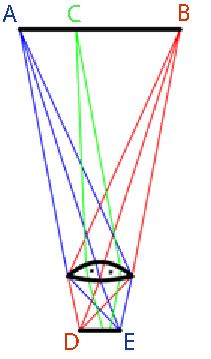
\includegraphics[width= 3.5cm]{Edge-ray}
  \end{center}
  \caption{\textbf{A lens receiving light.} The lens redirects light emitted from the source $\textrm{A}\textrm{B}$ to the receiver $\textrm{D}\textrm{E}$. 
Rays that leave the edges of the source hit the edges of the target (blue and red rays). Rays coming from the interior of the source will end at the interior of the target (green rays) \cite{wiki2}.}
  \label{fig:edge}
\end{figure}
\\ \indent
In $1985$ Mi{\~n}ano proved the principle by using the PS of the source and the target of an optical system \cite{minano1985two, minano1986design}. He proved the principle for systems in inhomogeneous media, where the index of refraction is a continuous function, so the map that connects the source and target phase spaces is a continuous map.
Indicating with $\map{M}{}{}(\point{P})$ the optical map of a point $\point{P}$, Mi{\~n}ano showed that if $\map{M}{}{}(\partial\mbox{\set{S}{}{}})=\partial\mbox{\set{T}{}{}}$ then 
$\map{M}{}{}(\mbox{\set{S}{}{}})=\mbox{\set{T}{}{}}$ and vice versa. 
%Note that the trajectory of two rays in PS cannot cross. 
The first version of the edge-ray principle \cite{minano1986design} can be enunciated in two-dimensions as follows:
\begin{lemma}{Edge-ray principle (version1)}\\ 
Suppose that:
\begin{itemize}
\item[a)] There are two regions \insieme{R}$_\textrm{s}$ and \insieme{R}$_\textrm{t}$ in source and target PS with the same area such that 
$$\map{M}{}{}(\partial\mbox{\insieme{R}}_\textrm{s}) = \map{M}{}{}(\partial\mbox{\insieme{R}}_\textrm{t});$$ 
\item[b)] The refractive-index distribution $\n$ is a continuous function; 
%\item[c)] They have the direction cosine with respect to the optical axis greater than $0$;
\end{itemize}
Then, the following relation holds: $$\map{M}{}{}(\mbox{\insieme{R}}_\textrm{s}) = \map{M}{}{}(\mbox{\insieme{R}}_\textrm{t}).$$
\end{lemma} 
The previous lemma claims that if there exist a map connecting the boundaries of two regions from source to target, also the interior of those regions are connected using the same map. Note that the second assumption in the previous lemma implies that the optical map is continuous in PS.
However, for some optical systems, as for instance the compound parabolic concentrator (CPC), the ray mapping in PS is not continuous. This is due to multiple reflections that rays can encounter with the reflectors and implies that some rays at the edge of the source could not be mapped into rays at the edges of the target \cite{davies1994edge}. \\ \indent 
In 1994 Ries and Rabl reformulated the edge-ray principle providing a version valid for all systems even if the ray map in PS is not continuous \cite{Ries:2}. 
Suppose that \insieme{R}$_\textrm{s}(\Pi)$ and $\mbox{\insieme{R}}_\textrm{t}(\Pi)$ are the regions, corresponding to path $\Pi$, at the source and the target PS, respectively. 
They showed that, for a given path $\Pi$, if the boundaries
$\partial\mbox{\insieme{R}}_\textrm{s}(\Pi)$ are mapped into the boundaries $\partial\mbox{\insieme{R}}_\textrm{t}(\Pi)$, then also the regions $\mbox{\insieme{R}}_\textrm{s}(\Pi)$ are mapped into the regions $\mbox{\insieme{R}}_\textrm{t}(\Pi)$.
Then, to map \set{S}{}{} to \set{T}{}{} it is necessary and sufficient that the first version of the edge ray principle is observed for all part of \set{S}{}{} and \set{T}{}{} defined by the number of reflections \cite{Ries:2}. 
\begin{lemma}{Edge-ray principle (generalized version)}\\
Let $(\Pi_\variabile{j})_{\variabile{j}=1, \cdots, \npath}$ denote all possible paths $\npath$.
Every possible path corresponds to a certain number of reflections or refractions.
Let us denote with \insieme{R}$_\textrm{s}(\Pi_\variabile{j})$ and 
\insieme{R}$_\textrm{t}(\Pi_\variabile{j})$ the regions at \set{S}{}{} and \set{T}{}{} associated to path $\Pi_\variabile{j}$ such that they are a partition of \set{S}{}{} and \set{T}{}{}, that is:
\begin{equation*}
\begin{aligned}
\mbox{\set{S}{}{}} &= \bigcup_{\variabile{j}=1}^{\npath} \mbox{\insieme{R}}_\textrm{s}(\Pi_\variabile{i}), \mbox{ with } \mbox{\insieme{R}}_\textrm{s}(\Pi_\variabile{j})\cap \mbox{\insieme{R}}_\textrm{s}(\Pi_\variabile{i}) = \emptyset \mbox{ for } \variabile{i}\neq \variabile{j}\\
\mbox{\set{T}{}{}} & \supset \bigcup_{\variabile{j}=1}^{\npath} \mbox{\insieme{R}}_\textrm{t}(\Pi_\variabile{i}), \mbox{ with } \mbox{\insieme{R}}_\textrm{t}(\Pi_\variabile{j})\cap \mbox{\insieme{R}}_\textrm{t}(\Pi_{\variabile{i}}) = \emptyset \mbox{ for } \variabile{j}\neq \variabile{i}.
\end{aligned}
\end{equation*} 
Then, to map a source region into a target, it is necessary and sufficient that the first version of the edge ray principle is observed for all parts of \set{S}{}{} and \set{T}{}{}: 
\begin{equation*}
\map{M}{}{}\big(\partial\mbox{\insieme{R}}_\textrm{s}(\Pi_{\variabile{j}})\big) = \partial\mbox{\insieme{R}}_\textrm{t}(\Pi_{\variabile{j}}), \quad \forall \variabile{j}\in\{1, \cdots, \npath\}.
\end{equation*}
\end{lemma}
Hence, the edge-ray principle constitutes a tool for designing ideal systems and, to this purpose, it is sufficient that the rays of $\partial\mbox{\insieme{R}}_\textrm{s}(\Pi)$ are transformed to the rays of $\partial\mbox{\insieme{R}}_\textrm{t}(\Pi)$ for every path $\Pi$ \cite{minano1992new}. 
\\ \indent Using the PS concept and the edge-ray principle we develop a new ray tracing method. 
A non-uniform distribution of the rays is constructed by developing a triangulation refinement at the source PS which is explained in the next section. 
The triangulation refinement provides more rays close to the boundaries of the regions $\mbox{\insieme{R}}_\textrm{s}(\Pi)$ each of them is formed by the rays that follow the same path $\Pi$.
\section{Phase space ray tracing}\label{sec:PS_raytracing}
PS ray tracing takes advantage of the fact that there exists an optical map
$
\map{M}{}{}: \mbox{\set{S}{}{}} \rightarrow \mbox{\set{T}{}{}}
$
 such that
\begin{equation}\label{eq:map1}
\map{M}{}{}(\variabile{q}_1,\variabile{p}_1)=(\variabile{q},\variabile{p}),
\end{equation} for every $(\variabile{q}_1,\variabile{p}_1)\in$ \set{S}{}{}.
For very simple systems, like the two-faceted cup, it is possible to determine an analytic expression for $\map{M}{}{}$.
This is not the case for most of the optical systems we deal with. In these cases it is necessary to implement ray tracing to calculate how light is distributed at the target.
As mentioned in the previous section, for some optical systems $\map{M}{}{}$ is not even continuous.
Nevertheless, given a path $\Pi$, the restriction of $\map{M}{}{}$ to \insieme{R}$_\textrm{s}$, 
i.e., $\map{M}{}{}(\Pi): \mbox{\insieme{R}}_\textrm{s}(\Pi)\rightarrow 
\mbox{\insieme{R}}_\textrm{t}(\Pi)$ is a continuous and bijective map. 
The edge ray principle guarantees that $\map{M}{}{}(\Pi)$ maps $\mbox{\insieme{R}}_\textrm{s}(\Pi)$ onto $\mbox{\insieme{R}}_\textrm{t}(\Pi)$ preserving topological features. In particular, the boundary $\partial\mbox{\insieme{R}}_\textrm{s}(\Pi)$ is mapped onto the boundary $\partial$\insieme{R}$_\textrm{t}(\Pi)$. %, see \cite{Ries, Davies, Minano}.
Employing the maps $\map{M}{}{}(\Pi)$ for all the possible paths $\Pi$, the output light distribution is determined. Therefore, the photometric variables at the target can be calculated.
\\ \indent The luminance $L(\variabile{q}, \variabile{p})$ at the target PS is given by:
\begin{equation}
\begin{aligned}
\label{eq:PSluminance}
L(\variabile{q}, \variabile{p}) &> 0  \mbox{  for } (\variabile{q}, \variabile{p})\in \mbox{\insieme{R}}_\textrm{t}(\Pi) \mbox{ for some path } \Pi,\\ \vspace{0.5 cm}
L(\variabile{q}, \variabile{p}) &= 0  \mbox{  otherwise}.
\end{aligned}
\end{equation}
The target intensity along a given direction $\variabile{p}=\const{const}$ is computed through an integration of the target luminance $L(\variabile{q}, \variabile{p})$ over $\variabile{q}$ and it is defined in \set{T}{}{}$\,$ by:
\begin{equation}
\label{eq:PSintensity}
I_{\textrm{PS}}(\variabile{p}) = \int_{\mbox{\set{Q}{}{}}}L(\variabile{q}, \variabile{p}) \textrm{d}\variabile{q}.
\end{equation}
Note that, while in the real space the intensity is defined as a function of the angular coordinate $\myangle$ (see Chapter \ref{chap:Illumination optics}), in PS the intensity is defined as a function of the direction coordinate $\variabile{p}=\n\sin(\myangle)$. The previous equation implies that, assuming a Lambertian source, the problem of computing the target intensity is reduced to the problem of calculating the boundaries
$\partial\mbox{\insieme{R}}_\textrm{t}(\Pi)$ for all possible paths $\Pi$. Hence, the intensity along the direction $\variabile{p}= \textrm{const.}$ is given by the sum of the interval lengths formed by the support of the luminance and the line $\variabile{p}=\textrm{const.}$ For example, if two intersection points between line $\variabile{p}= \textrm{const}$ and the boundary $\partial\mbox{\insieme{R}}_\textrm{t}(\Pi)$ are found, indicating their position coordinates with $\variabile{q}^\textrm{min}(\Pi,\variabile{p})$ and $\variabile{q}^\textrm{max}(\Pi,\variabile{p})$, where $\variabile{q}^\textrm{min}(\Pi,\variabile{p})<\variabile{q}^\textrm{max}(\Pi,\variabile{p})$ and, using (\ref{eq:PSluminance}), we obtain that (\ref{eq:PSintensity}) reduces to:
\begin{equation}\label{eta2}
I_{\textrm{PS}}(\variabile{p}) = \sum_{\Pi}\int_{\variabile{q}^\textrm{\,min}(\Pi, \variabile{p})}^{\variabile{q}^\textrm{\,max}(\Pi,\variabile{p})}L(\variabile{q}, \variabile{p})\textrm{d}\variabile{q} = \sum_{\Pi}\big (\variabile{q}^\textrm{max}(\Pi,\variabile{p})-\variabile{q}^\textrm{\,min}(\Pi,\variabile{p})\big )\,,
\end{equation}
where the sum is over all the possible paths and the second equation holds as we assume Lambertian source with $L=1$ in \insieme{R}$_\textrm{t}(\Pi).$ In case more than two intersection points occur, a generalized equation needs to be used for calculating the intensity. 
Note that for every single ray only one path is possible as we are assuming that all the lines are reflective lines.
Because of this, the regions \insieme{R}$_\textrm{t}(\Pi)$ do not overlap, i.e.
\begin{equation}
\bigcap_{\Pi}\mbox{\insieme{R}}_\textrm{t}(\Pi)= \emptyset,
\end{equation}
where the intersection is over all possible paths. \\ \indent
From equation (\ref{eta2}) we note that, using the PS structure, only the rays on the boundaries $\partial\mbox{\insieme{R}}_\textrm{t}(\Pi)$ are required for obtaining the target intensity profile.
%Instead of tracing the rays randomly (as in MC ray tracing) or following a regular source distribution (as in QMC ray tracing)
The aim is to construct a ray tracing procedure that allows us tracing less rays overall and more rays close to the discontinuity of the luminance, i.e., close to the boundaries $\partial\mbox{\insieme{R}}_\textrm{t}(\Pi)$.
To this purpose, we start from a triangulation made by only two triangles, then a triangulation refinement at \set{S}{}{} is defined as explained in the following. \\ \indent
The procedure starts with coordinates $(\variabile{q}_1^\variabile{k},\variabile{p}_1^\variabile{k})_{\variabile{k}=1, \cdots, 4}$ of the four corner points of \set{S}{}{}. For each of them, the corresponding path $(\Pi^\variabile{k})_{\variabile{k}=1, \cdots, 4}$ is calculated. Next, the grid is divided into two equal triangles joining two opposite vertices (in our simulation we always trace the diagonal north-west south-east to define the new triangles). For each triangle, the rays located at its corners are traced. If the paths corresponding to
those rays are not all equal, one or more boundaries
$\partial\mbox{\insieme{R}}_\textrm{t}(\Pi)$ are expected to cross the triangle.
In that case, the middle points $(\variabile{q}_1^\variabile{k},\variabile{p}_1^\variabile{k})_{\variabile{k}=5,6,7}$ of each side of the triangle are added and
the three corresponding rays are traced (unless they were already traced in the previous steps). Each refinement step leads to four new triangles (see Figure \ref{fig:refinement}).
 \begin{figure}[h]
 \begin{minipage}[h]{\textwidth}
\centering
    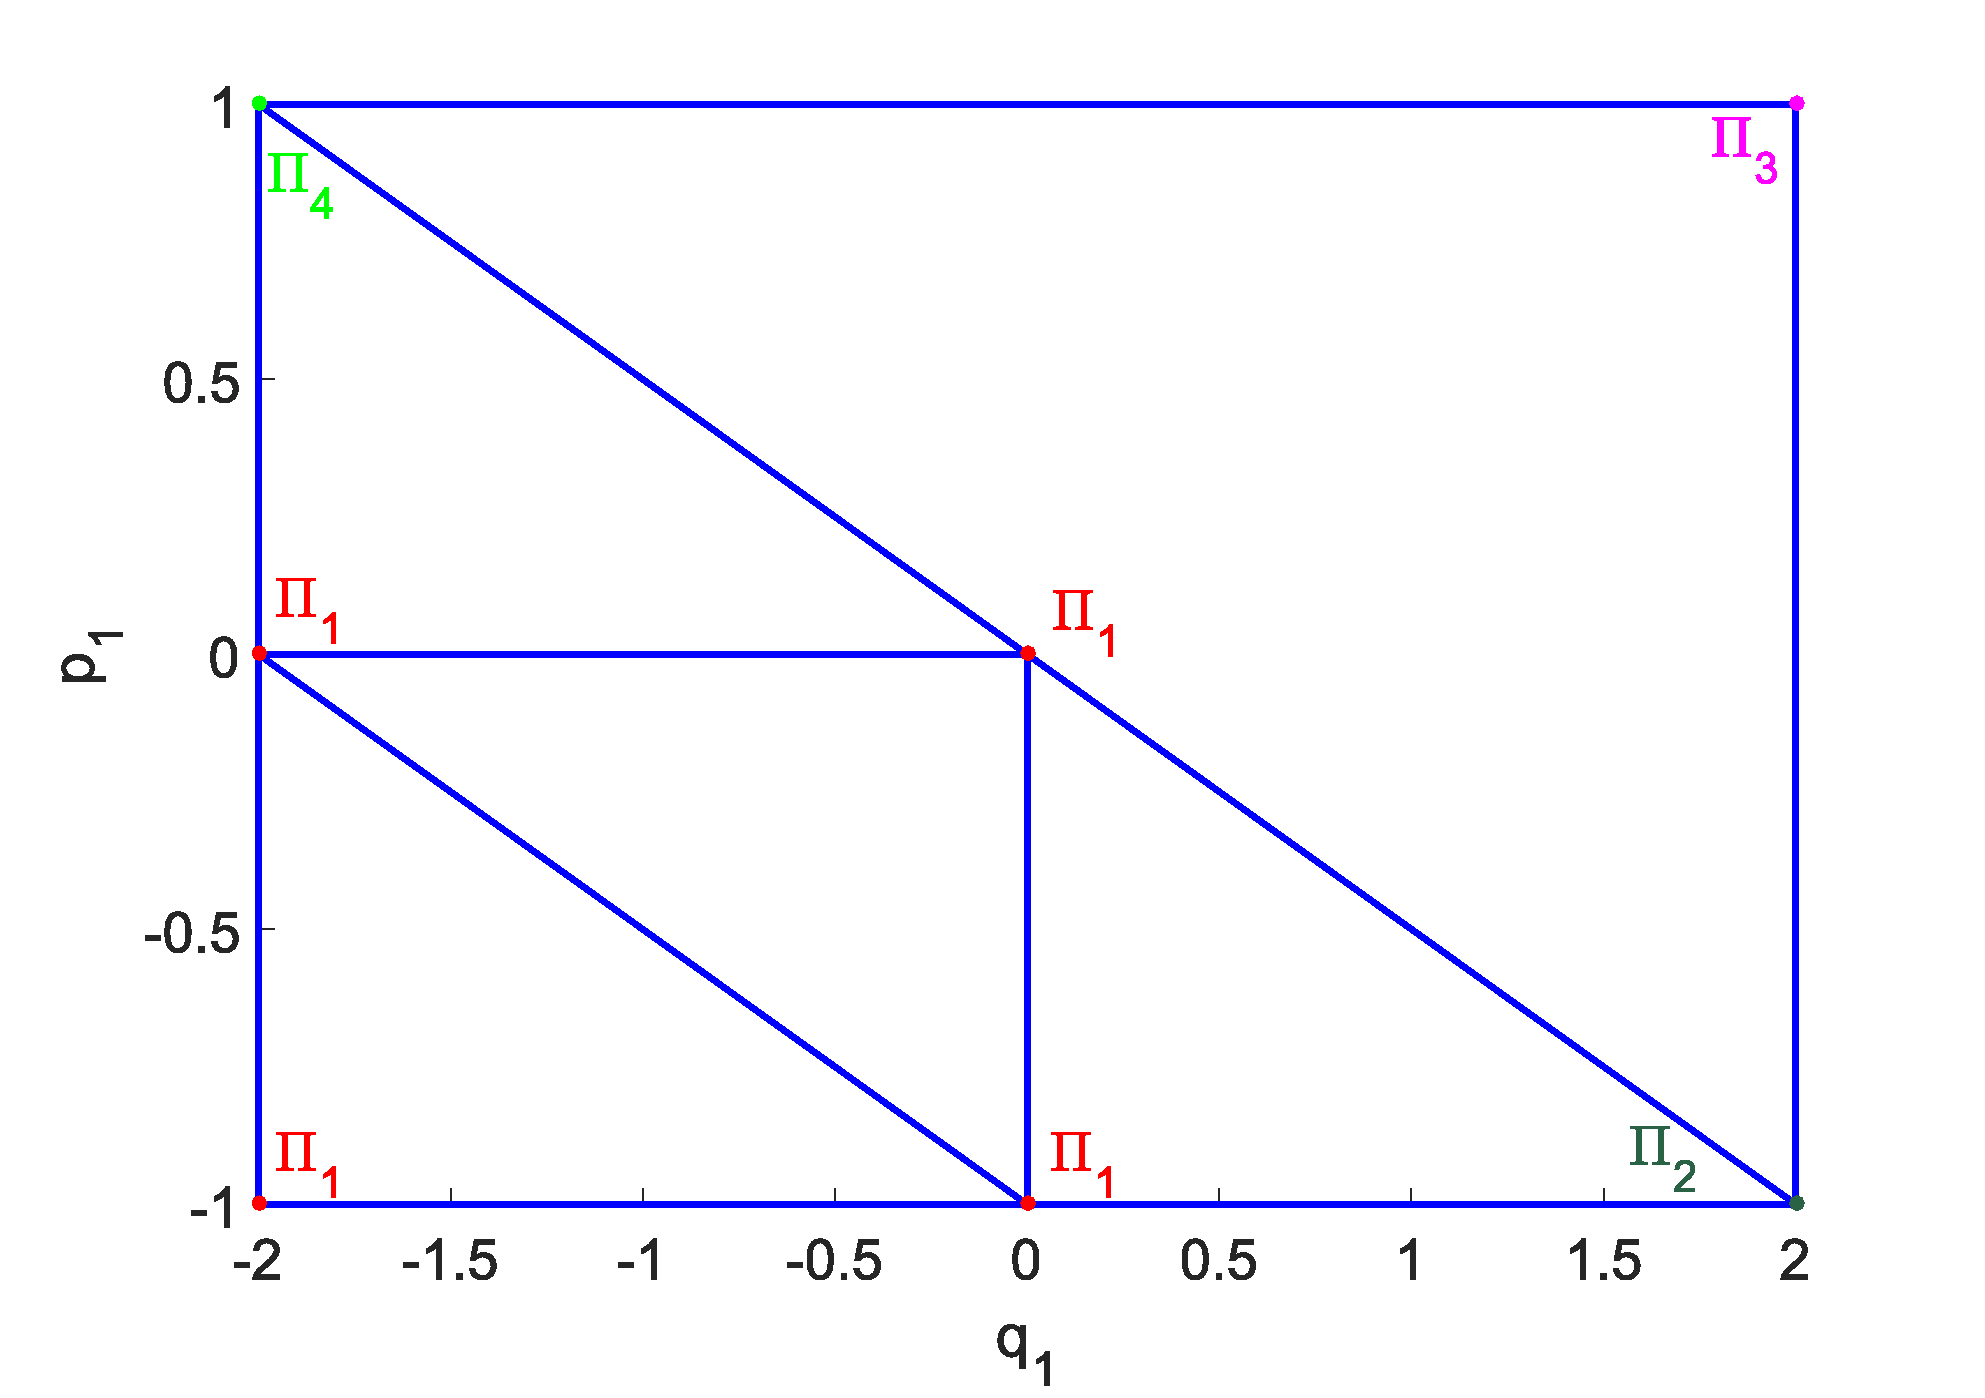
\includegraphics[width  = 0.9\textwidth]{region}
  \caption{\textbf{Triangulation refinement.} If the rays related to the vertices of the triangles follow a different path a new refinement step is required.
   Each refinement step leads to four new triangles.}
   %The parameters values are $\varepsilon_{\variabile{q}_{max}}~=~ 2$, $\varepsilon_{\variabile{p}_{max}}= 1$, $\varepsilon_{\variabile{q}_{min}}= 4$ and $\varepsilon_{\variabile{p}_{min}}=2$.}
  \label{fig:refinement}
\end{minipage}\\
\begin{minipage}[h]{\textwidth}
\centering
    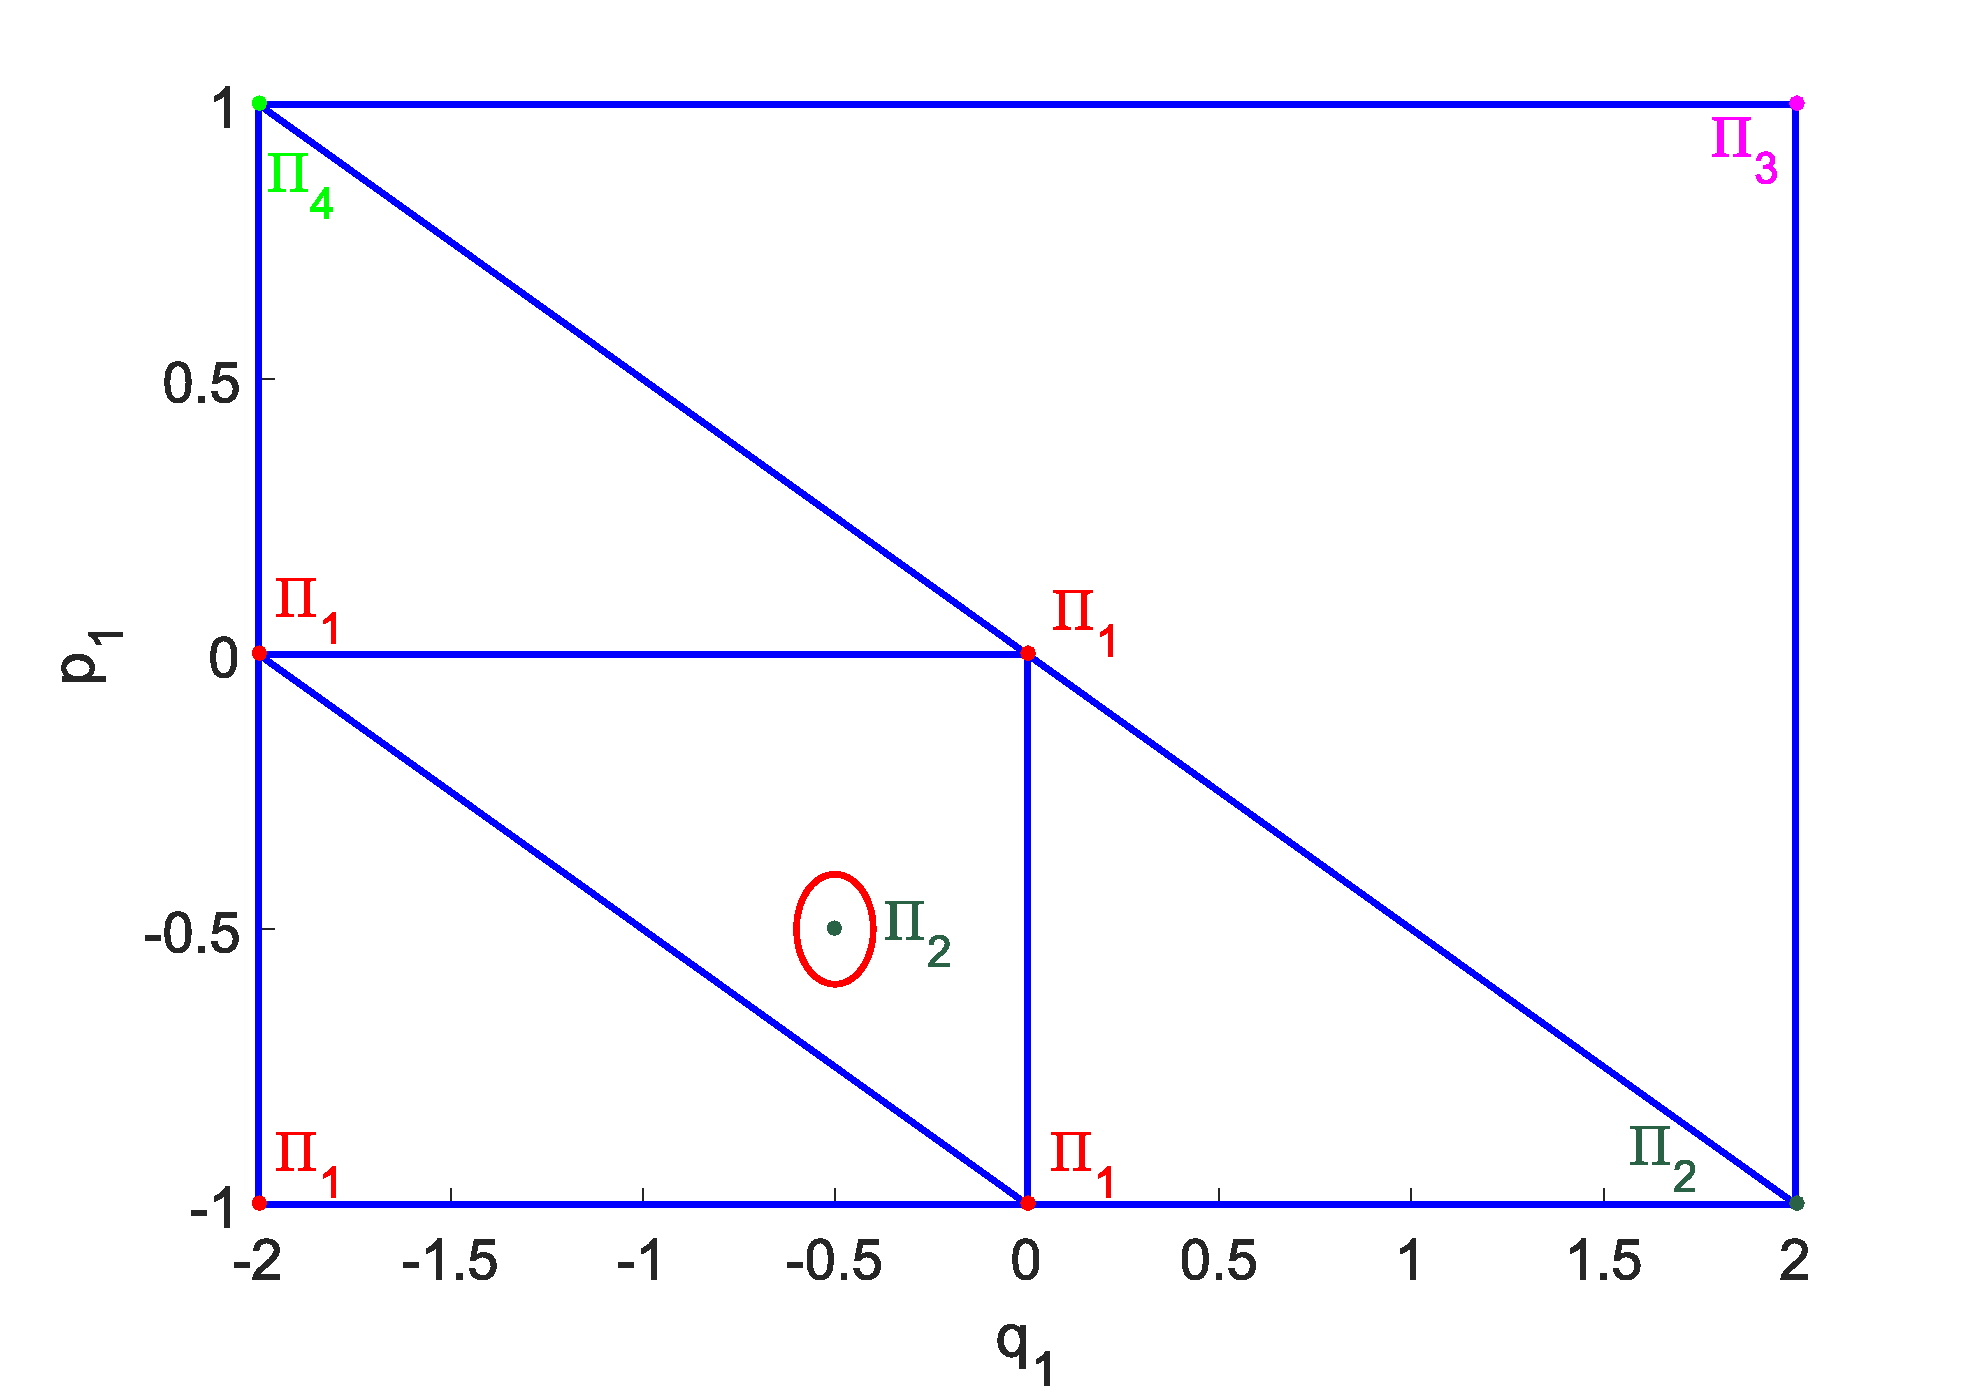
\includegraphics[width  = 0.9\textwidth]{region_inside}
  \caption{\textbf{Triangulation refinement.} The red line encloses a region of rays that follow the path $\Pi_2$ and is completely located inside a triangle.
  The algorithm is not able to detect that region and, a further refinement is required.}
   \label{fig:region inside}
\end{minipage}
  \end{figure} \\ \indent
When all the rays corresponding to the corners of each triangle have the same path, it is not necessary to refine the triangles anymore.
Since the triangles very close to the boundaries are always crossed by at least a boundary, at least two different paths are found for the rays at the vertices of those triangles. 
Because of this, the procedure could continue infinitely, therefore, two parameters $\varepsilon_\variabile{q}^\textrm{min}$ and $\varepsilon_\variabile{p}^\textrm{min}$ are introduced to defined a stopping criterion.
The algorithm stops when the length of the sides of the triangles is smaller than $\varepsilon_\variabile{q}^\textrm{min}$ and $\varepsilon_\variabile{p}^\textrm{min}$ in $\variabile{q}$ and $\variabile{p}$ direction. \\ \indent 
We indicate all the possible paths with $(\Pi_{\variabile{j}})_{\variabile{j}=1, \cdots, \npath}$ where $\npath$ is the maximum number of paths\footnote{We remind the reader that we indicate with $\Pi^\variabile{k} = \Pi(\variabile{q}_1^\variabile{k},\variabile{p}_1^\variabile{k})$ the path followed by rays with coordinates $(\variabile{q}_1^\variabile{k},\variabile{p}_1^\variabile{k})$ in source PS. Note that it
can happen that $\Pi^\variabile{k}= \Pi^\variabile{h}$ for $\variabile{k}\neq\variabile{h}.$
With $(\Pi_{\variabile{j}})_{\variabile{j}=1, \cdots, \npath}$ we indicate all the possible $\npath$ paths that can occur, therefore $\Pi_{\variabile{i}}\neq\Pi_{\variabile{j}}$ if $\variabile{i}\neq\variabile{j}$.} (\npath = 5 for the two-faceted cup in Figure \ref{fig:cup}).
If the size of the triangles is too big, it can happen that a region formed by rays that follow a path $\Pi_\variabile{j}$ is located completely inside a triangle whose vertices are related to another path $\Pi_\variabile{i}$ with $\variabile{j} \neq  \variabile{i}$, see Figure \ref{fig:region inside}.
To avoid this, two parameters $\varepsilon_\variabile{q}^{\textrm{max}}$ and $\varepsilon_\variabile{p}^{\textrm{max}}$ are defined for the $\variabile{q}_1$-axis and the $\variabile{p}_1$-axis, respectively.
When the length of the sides of the triangle are greater than these parameters, a new triangle is defined even if its vertices correspond to the same path.
The values of the parameters $\varepsilon_\variabile{q}^\textrm{min}$, $\varepsilon_\variabile{p}^\textrm{min}$, $\varepsilon_\variabile{q}^\textrm{max}$ and $\varepsilon_\variabile{p}^\textrm{max}$ determine the number of rays traced.
Thus, on the one hand, decreasing $\varepsilon_\variabile{q}^\textrm{min}$ and $\varepsilon_\variabile{p}^\textrm{min}$ more rays close to the boundaries are traced;
on the other hand, decreasing the values of $\varepsilon_\variabile{q}^\textrm{max}$ and $\varepsilon_\variabile{p}^\textrm{max}$ more rays in the interior of the regions are traced. \\ \indent The triangulation refinement is provided by Algorithm \ref{alg:triangulation} which uses the two recursive functions L$\footnotesize{\textrm{EFT}}$ T$\footnotesize{\textrm{RIANGLE}}$ and  R$\footnotesize{\textrm{IGHT}}$ T$\footnotesize{\textrm{RIANGLE}}$.
The function L$\footnotesize{\textrm{EFT}}$ T$\footnotesize{\textrm{RIANGLE}}$ is defined in Algorithm \ref{alg:left_triangle} (see Figure \ref{fig:triangulation_left}). 
A similar procedure gives the function R$\footnotesize{\textrm{IGHT}}$ T$\footnotesize{\textrm{RIANGLE}}$ (see Figure \ref{fig:triangulation_right}).
\begin{algorithm}[h]
\caption{Triangulation refinement algorithm}\label{alg:triangulation}
Initialize $\varepsilon_{\variabile{q}}^{\textrm{min}}, \varepsilon_{\variabile{q}}^{\textrm{max}}, \varepsilon_{\variabile{p}}^{\textrm{min}},$ and
 $\varepsilon_{\variabile{p}}^{\textrm{max}}$, Ray = [empty];\\
Define a structure that contains related data in fields. \\
\Comment $\varepsilon_{\variabile{q}}^{\textrm{min}}, \varepsilon_{\variabile{q}}^{\textrm{max}}, \varepsilon_{\variabile{p}}^{\textrm{min}},$ and
 $\varepsilon_{\variabile{p}}^{\textrm{max}}$ are fixed parameters needed to stop the procedure\\
\Comment Ray: structure that contains all the data of rays traced (i.e., position, direction and path).
\begin{algorithmic}[1]
%\Procedure{Triangulation refinement}{}
\State $(\variabile{q}_1^1, \variabile{p}_1^1)= (-\variabile{a}, -1)$ \Comment \mbox{left bottom corner of source PS \;}
\State $(\variabile{q}_1^2, \variabile{p}_1^2) = (\variabile{a}, -1)$ \Comment \mbox{right bottom corner of source PS}
\State $(\variabile{q}_1^3, \variabile{p}_1^3)  = (\variabile{a}, 1)$ \Comment \mbox{right upper corner of source PS\;\;}
\State $(\variabile{q}_1^4, \variabile{p}_1^4) = (-\variabile{a}, 1) $ \Comment \mbox{left upper corner of source PS\;\;\;\;\,}
\For{$ \variabile{k}= 1 \to 4 $}
\State Trace the ray with initial coordinates $(\variabile{q}_1^\variabile{k}, \variabile{p}_1^{\variabile{k}})$ in \set{S}{}{};
\State Calculate the corresponding path $\Pi^{\variabile{k}}$; $\qquad \qquad \qquad \qquad \qquad \qquad \qquad \qquad\quad$
\Comment Store the information found in the structure Ray;
\State $\textrm{Ray}.\variabile{q}= [\mbox{\textrm{Ray}}.\variabile{q}, \variabile{q}_1^\variabile{k}]$;
\State $\textrm{Ray}.\variabile{p}= [\mbox{\textrm{Ray}}.\variabile{p}, \variabile{p}_1^\variabile{k}]$;
\State $\textrm{Ray}.\Pi = [\mbox{\textrm{Ray}}.\Pi, \Pi^{\variabile{k}}]$;
\EndFor
\State VL $= [1, 2, 4]$ \Comment{VL vertices of the left triangle\;\,\,\,}
\State VR $= [2,3, 4]$   \Comment{VR vertices of the right triangle}
\State \Call{Left Triangle}{VL, Ray, $\varepsilon_{\variabile{q}_1}^{\textrm{min}}, \varepsilon_{\variabile{q}_1}^{\textrm{max}}, \varepsilon_{\variabile{p}_1}^{\textrm{min}}, \varepsilon_{\variabile{p}_1}^{\textrm{max}}$}\Comment{Refine the left triangle\;\,\,} 
\State \Call{Right Triangle}{VR, \textrm{Ray}, $\varepsilon_{\variabile{q}_1}^{\textrm{min}}, \varepsilon_{\variabile{q}_1}^{\textrm{max}}, \varepsilon_{\variabile{p}_1}^{\textrm{min}}, \varepsilon_{\variabile{p}_1}^{\textrm{max}}$} \Comment{Refine the right triangle} \\
\Return Ray;
%\EndProcedure
\end{algorithmic}
\end{algorithm}
\begin{algorithm}[h]
\caption{Algorithm for the refinement of the left triangles}\label{alg:left_triangle}
\begin{algorithmic}[1]
\Procedure{Left triangle}{VL, \textrm{Ray}, $\varepsilon_{\variabile{q}}^{\textrm{min}}, \varepsilon_{\variabile{q}}^{\textrm{max}}, \varepsilon_{\variabile{p}}^{\textrm{min}}, \varepsilon_{\variabile{p}}^{\textrm{max}}$}
\State $\textrm{VL}= [1,2,4]$
\State $\variabile{q}_1^1= \textrm{Ray}.\variabile{q}(\textrm{VL}(1))$, $\variabile{p}_1^1= \textrm{Ray}.\variabile{p}(\textrm{VL}(1))$
\State $\variabile{q}_1^2= \textrm{Ray}.\variabile{q}(\textrm{VL}(2))$, $\variabile{p}_1^2= \textrm{Ray}.\variabile{p}(\textrm{VL}(2))$
\State $\variabile{q}_1^3= \textrm{Ray}.\variabile{q}(\textrm{VL}(3))$, $\variabile{p}_1^3= \textrm{Ray}.\variabile{p}(\textrm{VL}(4))$
\State $\textrm{dist}_\variabile{q}= \mbox{$|\variabile{q}_1^2-\variabile{q}_1^1|$}$
\State $\textrm{dist}_\variabile{p}= \mbox{$|\variabile{p}_1^{3}-\variabile{p}_1^1|$}$
\State RefineTriangle $=$  false;
\State DifferentPath $=$  false;
\If{$\textrm{dist}_\variabile{q}>\varepsilon_{\variabile{q}}^{\textrm{max}} $ or $\textrm{dist}_\variabile{p} >\varepsilon_{\variabile{p}}^{\textrm{max}}$}
\State RefineTriangle $=$  true;
\EndIf
\For{$ \variabile{k} = 1 \to 2 $}
\If{$\Pi^{\variabile{k}} \neq \Pi^{\variabile{k}+1}$}
\State DifferentPath $=$  true;
\EndIf
\EndFor
\If{$\textrm{dist}_\variabile{q}>\varepsilon_{\variabile{q}}^{\textrm{min}}$ or $\textrm{dist}_\variabile{p}>\varepsilon_{\variabile{p}}^{\textrm{min}}$}
\State RefineTriangle $=$  DifferentPath;
\Else
\If{(DifferentPath is true)}
\State \textrm{Ray}(\textrm{VL}).boundary $=$ true; \Comment{A boundary crosses the triangle}
\EndIf
\EndIf
\If {(RefineTriangle is true)}
\State Define the points at the middle of each side of the triangle
\State $(\variabile{q}_1^5, \variabile{p}_1^5) = ((\variabile{q}_1^1+\variabile{q}_1^2)/2, \variabile{p}_1^1)$
\State $(\variabile{q}_1^6, \variabile{p}_1^6) = (\variabile{q}_1^5, (\variabile{p}_1^1+\variabile{p}_1^2)/2)$
\State $(\variabile{q}_1^7, \variabile{p}_1^7) = (\variabile{q}_1^1, \variabile{p}_1^6)$
\For {$\variabile{k} = 5 \to 7 $}
\If {The ray with coordinates $(\variabile{q}_1^\variabile{k}, \variabile{p}_1^\variabile{k})$ is not traced yet}
\State Trace the ray with initial coordinates: $(\variabile{q}_1^\variabile{k}, \variabile{p}_1^\variabile{k})$ in PS;
\State Compute the corresponding path $\Pi^{\variabile{k}}$;
\State Store the ray's coordinates $\mbox{\textrm{Ray}}.\variabile{q}= [\mbox{Ray}.\variabile{q}, \variabile{q}_1^\variabile{k}]$;
\State Store the ray path $\mbox{\textrm{Ray}}.\Pi= [\mbox{\textrm{Ray}}.\Pi, \Pi^{\variabile{k}}]$;
\EndIf
\EndFor
\State\Return{\Call{Left Triangle}{$[\textrm{VL}(1),5, 7], \mbox{\textrm{Ray}}, \varepsilon_{\variabile{q}}^{\textrm{min}}, \varepsilon_{\variabile{q}}^{\textrm{max}}, \varepsilon_{\variabile{p}}^{\textrm{min}}, \varepsilon_{\variabile{p}}^{\textrm{max}}$}};
\State\Return{\Call{Left Triangle}{$[5,\textrm{VL}(2), 6], \mbox{\textrm{Ray}}, \varepsilon_{\variabile{q}}^{\textrm{min}}, \varepsilon_{\variabile{q}}^{\textrm{max}}, \varepsilon_{\variabile{p}}^{\textrm{min}}, \varepsilon_{\variabile{p}}^{\textrm{max}}$}};
\State\Return{\Call{Left Triangle}{$[7,6,\textrm{VL}(3)], \mbox{\textrm{Ray}}, \varepsilon_{\variabile{q}}^{\textrm{min}}, \varepsilon_{\variabile{q}}^{\textrm{max}}, \varepsilon_{\variabile{p}}^{\textrm{min}}, \varepsilon_{\variabile{p}}^{\textrm{max}}$}};
\State\Return{\Call{Right Triangle}{$[5,6, 7], \mbox{\textrm{Ray}}, \varepsilon_{\variabile{q}}^{\textrm{min}}, \varepsilon_{\variabile{q}}^{\textrm{max}}, \varepsilon_{\variabile{p}}^{\textrm{min}}, \varepsilon_{\variabile{p}}^{\textrm{max}}$}};
\EndIf \\
\Return \textrm{Ray};
\EndProcedure
\end{algorithmic}
\end{algorithm}
\\ \indent Figure \ref{fig:triangulation_refinement} shows an example of a triangulation refinement at the source PS of the two-faceted cup in Figure \ref{fig:cup}. 
For this optical system, the width of the $\variabile{q}_1$-axis in source PS is two times the width of the $\variabile{p}_1$-axis.
Thus, our choice is $\varepsilon_\variabile{p}^{\textrm{min}}=\frac{1}{2}\varepsilon_\variabile{q}^{\textrm{min}}$ and $\varepsilon_\variabile{p}^{\textrm{max}} = \frac{1}{2}\varepsilon_\variabile{q}^{\textrm{max}}$
with $\varepsilon_\variabile{q}^{\textrm{min}}=0.1$ and $\varepsilon_\variabile{q}^{\textrm{max}}=1$.
 \begin{figure}[h]
 \begin{minipage}[h]{0.48\textwidth}
\centering
    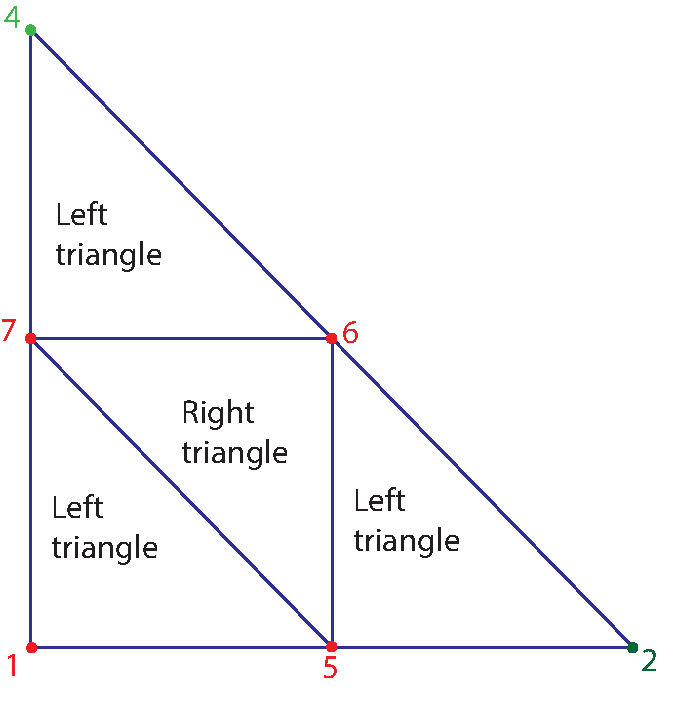
\includegraphics[width=\textwidth]{Triangulation_left}
    \caption{\textbf{Left triangulation refinement.} The algorithm used is the recursive function L$\footnotesize{\textrm{EFT}}$ T$\footnotesize{\textrm{RIANGLE}}$.}
    \label{fig:triangulation_left}
\end{minipage}
\hfill
\begin{minipage}[h]{0.48\textwidth}
\centering
    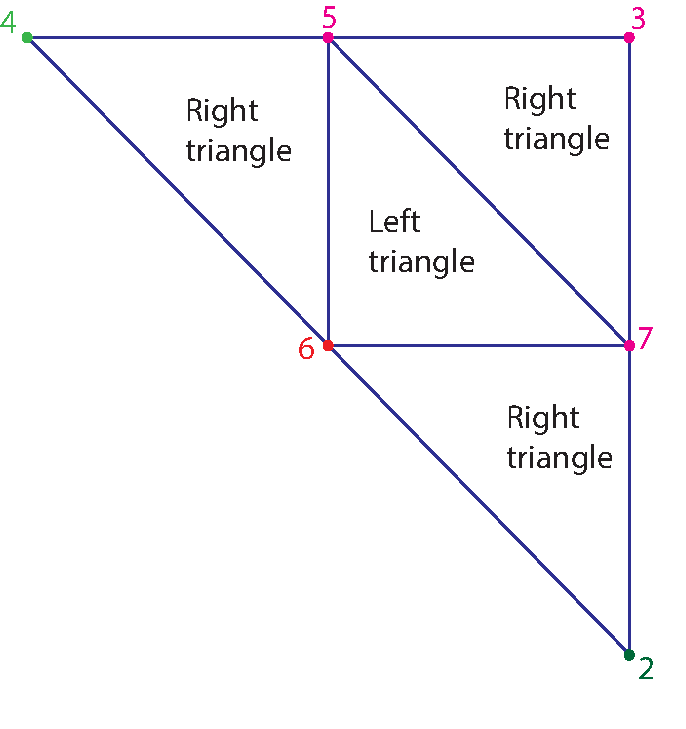
\includegraphics[width = \textwidth]{Triangulation_right}
    \caption{\textbf{Right triangulation refinement.} The algorithm used is the recursive function R$\footnotesize{\textrm{IGHT}}$ T$\footnotesize{\textrm{RIANGLE}}$.}
    \label{fig:triangulation_right}
\end{minipage}
\end{figure}
\hfill
\begin{figure}[h]
  \begin{center}
  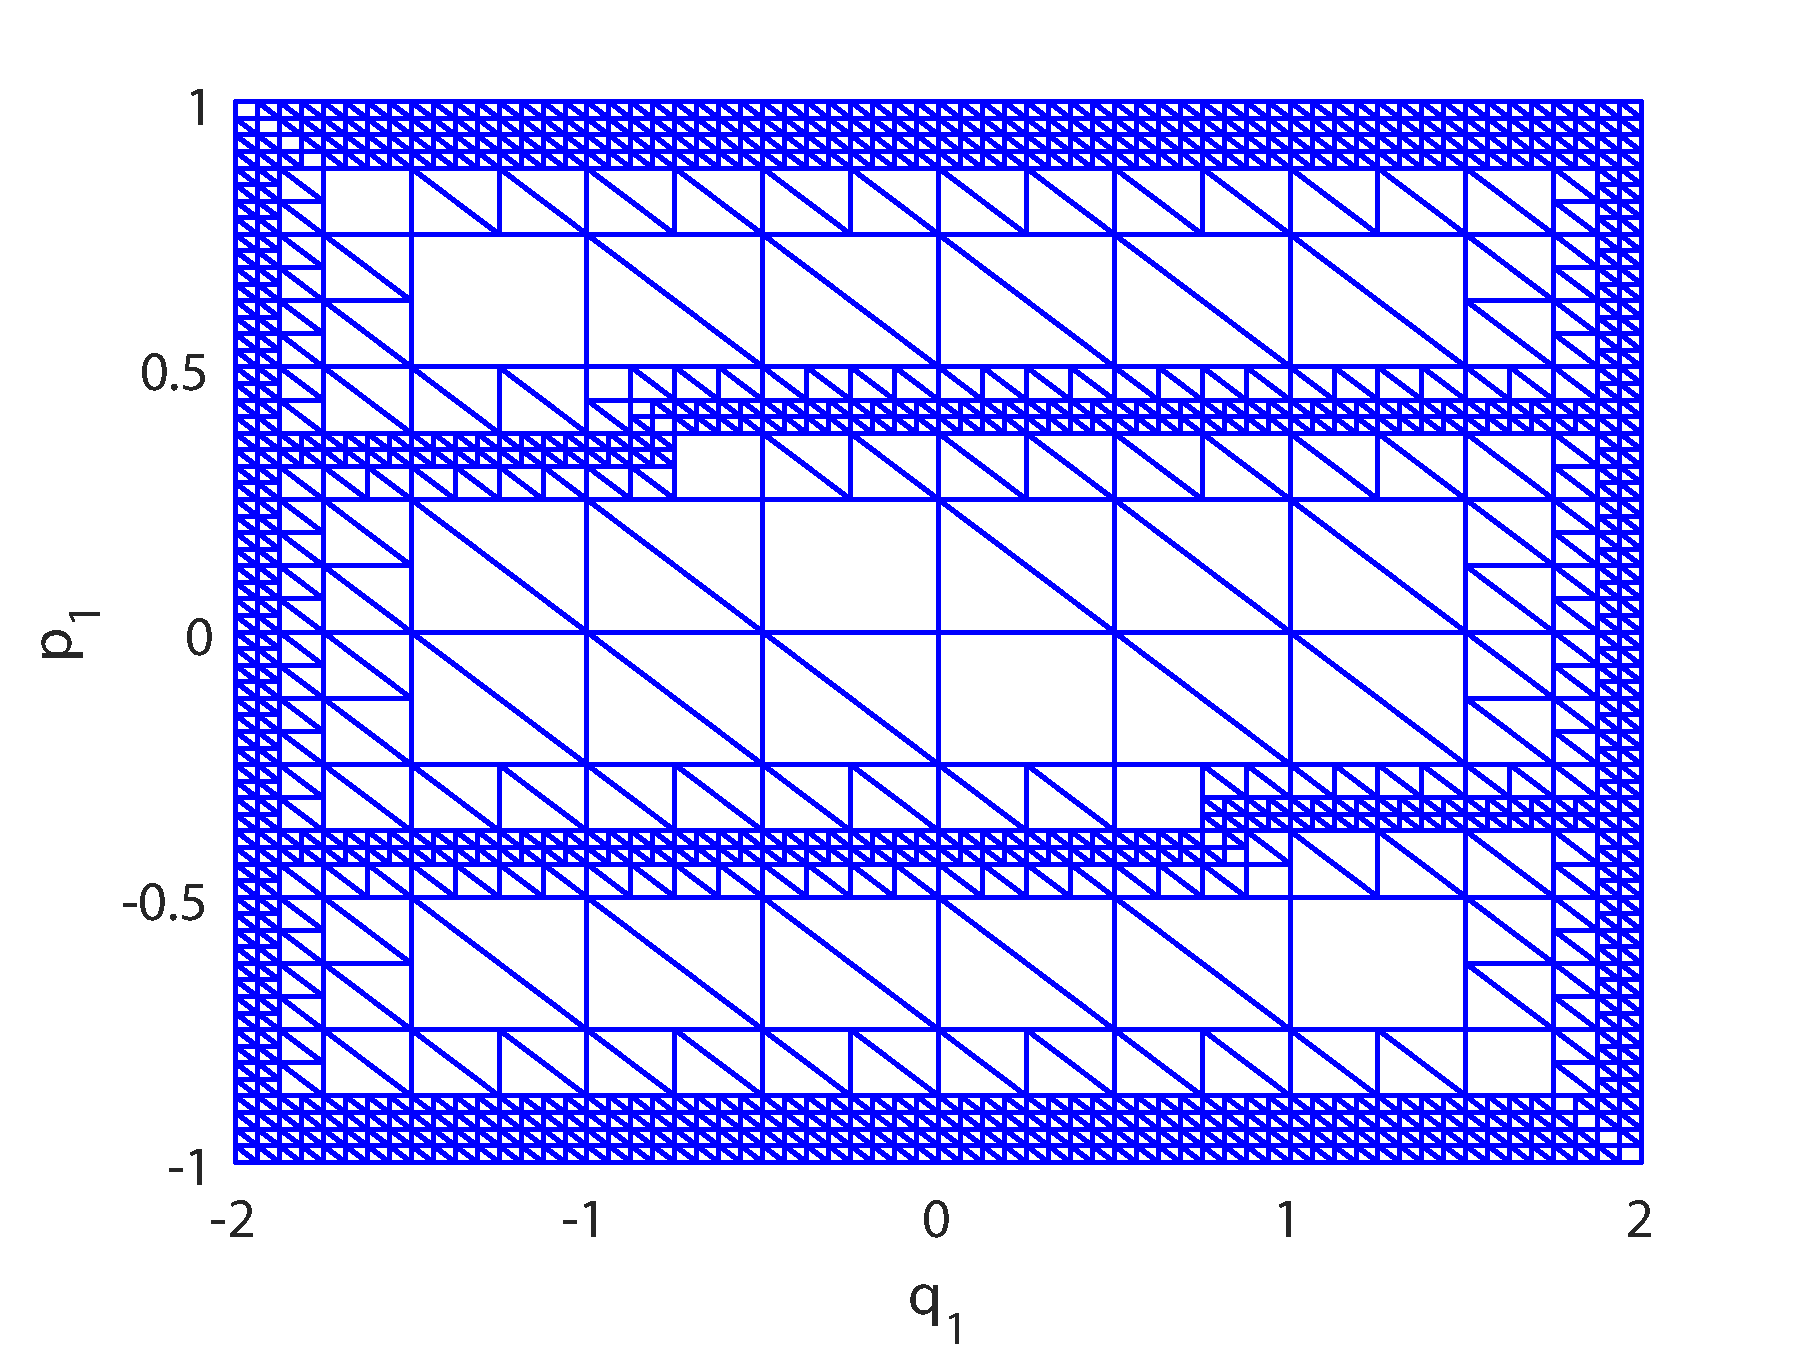
\includegraphics[width=0.9\textwidth]{triangulation_source}
  \end{center}
  \caption{\textbf{Triangulation refinement of source phase space.} 
Near the boundaries more rays are traced.
    The values of the parameters are $\varepsilon_{\variabile{q}_1}^\textrm{min}~=~ 0.1$, $\varepsilon_{\variabile{q}_1}^\textrm{max}~=~1$, $\varepsilon_{\variabile{p}_1}^\textrm{min}= \varepsilon_{\variabile{q}_1}^\textrm{min}/2$ and $\varepsilon_{\variabile{p}_1}^\textrm{max} = \varepsilon_{\variabile{q}_1}^\textrm{max}/2$.}
   \label{fig:triangulation_refinement}
  \end{figure}
\\ \indent The triangulation refinement allows finding \textit{all} the possible paths $(\Pi_\variabile{j})_{\variabile{j} = 1, \cdots, \npath}$ and their corresponding regions \insieme{R}$_\textrm{s}(\Pi_\variabile{j})_{\variabile{j} = 1, \cdots, \npath}$. Using the edge-ray principle, we conclude that also the regions $\mbox{\insieme{R}}_\textrm{t}(\Pi_\variabile{j})_{\variabile{j} = 1, \cdots, \npath}$ at the target are determined and only the rays close to the boundaries
$\partial\mbox{\insieme{R}}_\textrm{s}$ need to be considered to obtain the target ray distribution.
\section{Conclusions}
In this chapter we introduced the PS concept. 
We explained a new ray tracing method based on the source and the target PS representation. 
In PS every point corresponds to a unique ray. 
The coordinates of every point correspond to the initial ray position $\variabile{q}_1$ and the initial ray direction $\variabile{p}_1 = \sin\myangle_1$ (as $\n_1 = 1$) expressed with respect to the normal of the source. The method also takes into account the paths followed by every ray traced.
Considering only reflection, every single ray follows only one path and, therefore, the PS regions do not overlap. 
\\ \indent
As an example, we provided the source and the target PS representation of the two-faceted cup.
The edge-ray principle guarantees that all the rays that follow the same path are located in the same regions in PS. If we know these regions at the source we can determine the corresponding regions at the target. 
It is sufficient to map the boundaries at the source $\partial\mbox{\insieme{R}}_\textrm{s}(\Pi)$ to obtain their corresponding target boundaries $\partial\mbox{\insieme{R}}_\textrm{t}(\Pi)$. \\ \indent
The boundaries $\partial\mbox{\insieme{R}}_\textrm{t}(\Pi)$ are particularly relevant because there the luminance jumps from $0$ to a positive value. 
Assuming a Lambertian source, only the rays at the boundaries are needed to compute the target intensity. 
Based on this idea, a triangulation in \set{S}{}{} is constructed such that the rays closest to $\partial\mbox{\insieme{R}}_\textrm{s}(\Pi)$
are selected and more rays in their vicinity are created to get progressively better estimates of the boundaries.
\\ \indent In Figure \ref{fig:three_distributions} we show three different ray distributions on the source PS of the two-faceted cup. In Figure \ref{fig:mc_sample}, $10^3$ random points are shown. MC ray tracing is based on this random distribution of the initial rays set. In Figure \ref{fig:qmc_sample}, $10^3$ points of a two-dimensional Sobol sequence are shown. 
Since Sobol sequences are defined in a unit square, we scaled it such that all the source PS \set{S}{}{}$=[-2, 2]\times[-1, 1]$ is covered by rays. Such regular distributions can lead to several advantages for the computation of the target intensity (see Section \ref{sec:QMC}). Finally, Figure \ref{fig:ps_sample} shows a non-uniform distribution of rays at the source PS on which PS ray tracing is based. Such distribution is obtained from the triangulation refinement explained in the previous section. The procedure requires tracing more rays close to the boundaries $\partial\mbox{\insieme{R}}_\textrm{s}(\Pi)$ and only few rays in their interior. From the edge ray-principle, we obtain that these rays will be located close to the boundaries $\partial\mbox{\insieme{R}}_\textrm{t}(\Pi)$ of the regions at the target PS. The target PS intensity is calculated using only the rays that are located at the boundaries $\partial\mbox{\insieme{R}}_\textrm{t}(\Pi)$. Thus, in order to obtain the intensity profile at the target, the boundaries $\partial\mbox{\insieme{R}}_\textrm{t}(\Pi)$ need to be determined.\\ \indent 
In the next chapter we provide two different approaches to find $\partial\mbox{\insieme{R}}_\textrm{t}(\Pi)$ using a set of rays given by the triangulation refinement.
\begin{figure}[h]
 \begin{subfigure}[t]{\textwidth}
\centering
    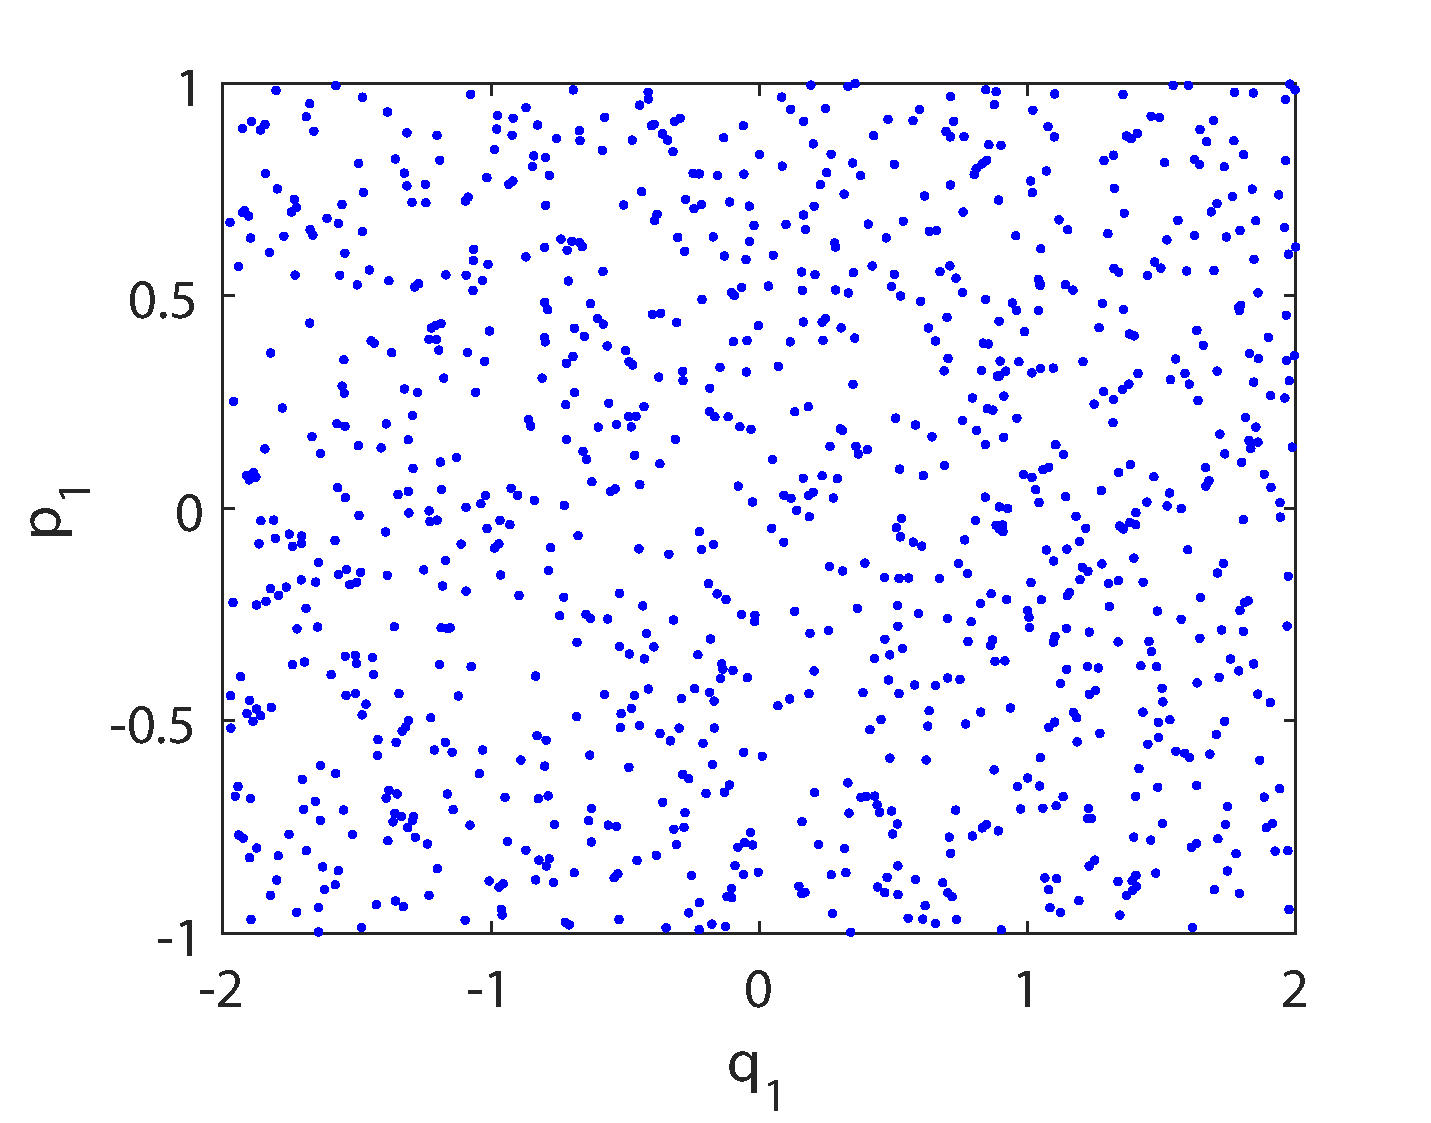
\includegraphics[width=0.57\textwidth]{MC_source_cup}
    \caption{\textbf{MC grid.} $10^3$ rays randomly distributed (MC ray tracing).}
    \label{fig:mc_sample}
\end{subfigure}
\hfill
\\
\begin{subfigure}[t]{\textwidth}
\centering
    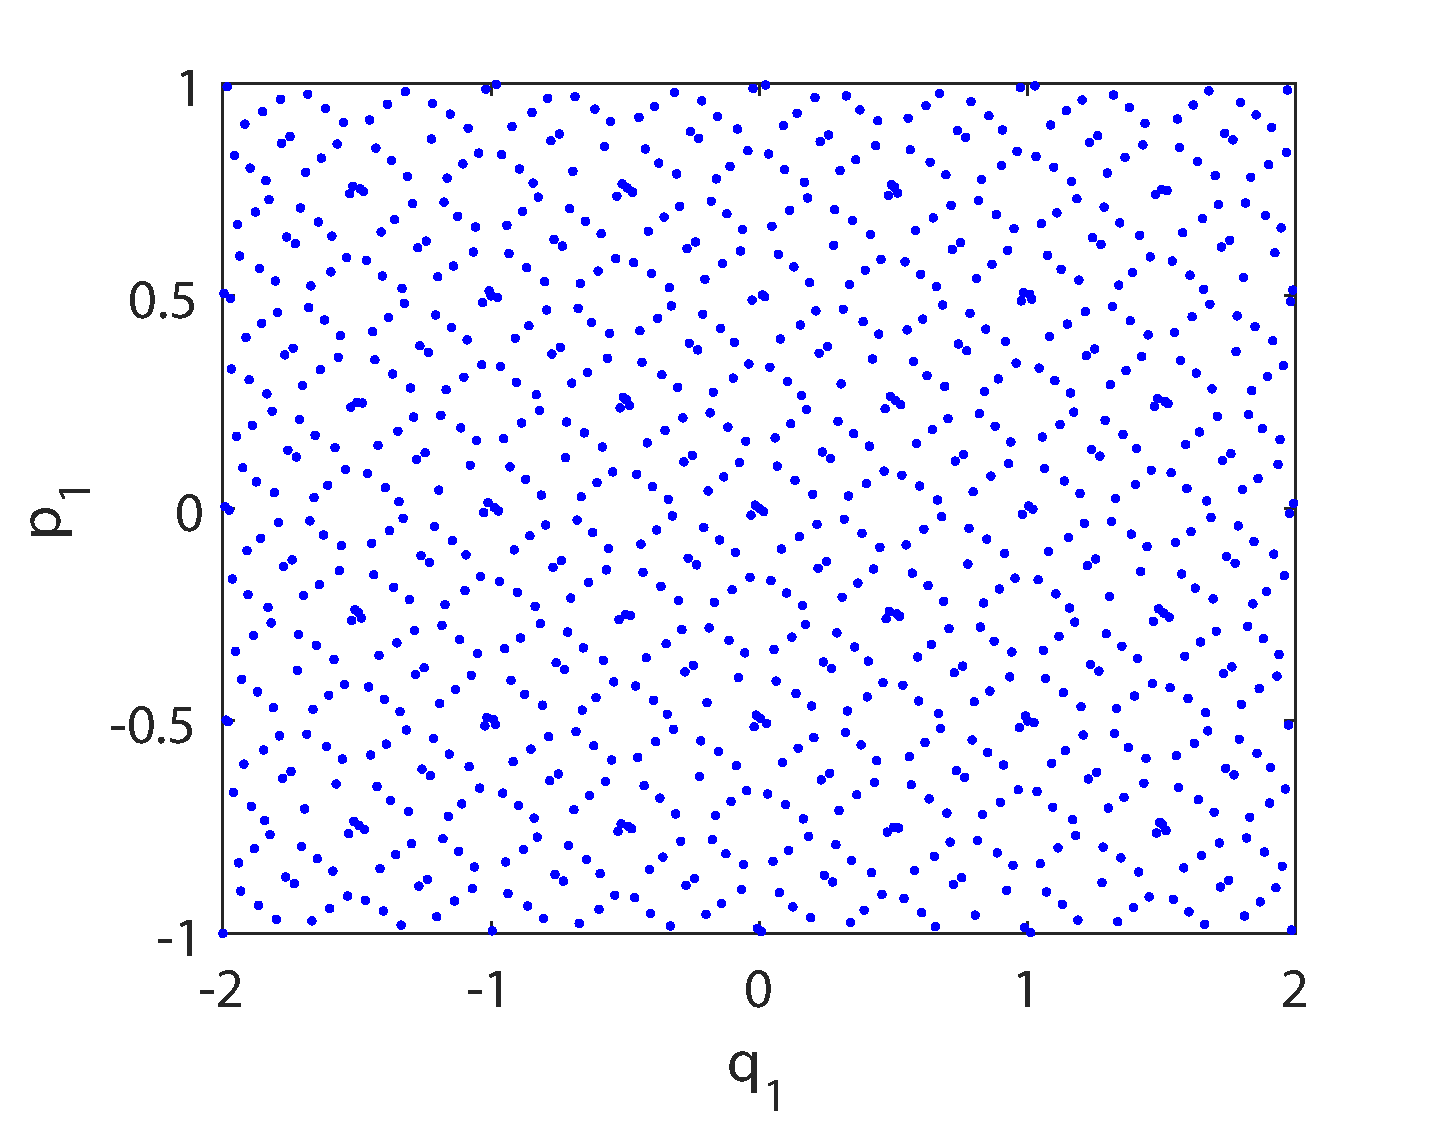
\includegraphics[width = 0.57\textwidth]{QMC_source_cup}
    \caption{\textbf{QMC grid}. $10^3$ rays distributed as the point of a Sobol sequence (QMC ray tracing).}
    \label{fig:qmc_sample}
\end{subfigure}
\hfill
\begin{subfigure}[t]{\textwidth}
\centering
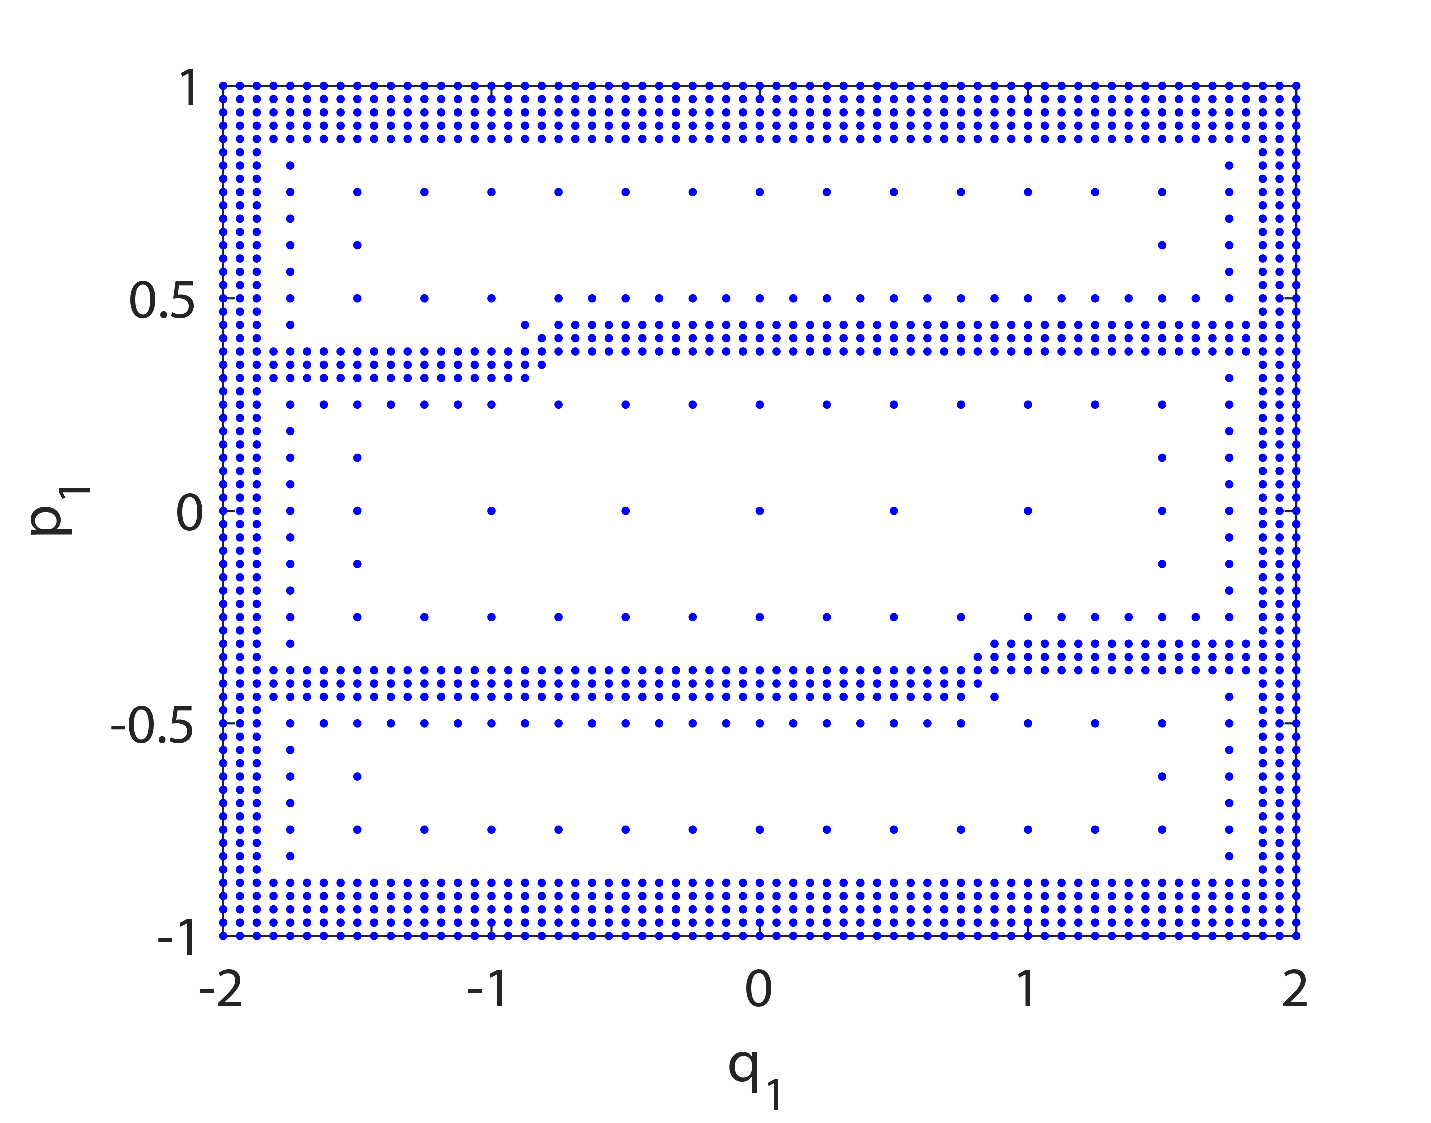
\includegraphics[width=0.57\textwidth]{PS_source_cup1_rev}
\caption{\textbf{PS grid.} $1.5\cdot10^3$ rays distributed using the triangulation refinement (PS ray tracing).}
\label{fig:ps_sample}
\end{subfigure}
\caption{\textbf{Three different ray distributions.} Source PS of the two-faceted cup.}
\label{fig:three_distributions}
\end{figure}

% Compare all the PS
% Definition of luminance intensity and etendue
%\indent A similar method as described in this chapter is presented by Moore, \cite{moore2013methods}. In Moore's method each ray leaves the source at the same position while the angle coordinate changes. The path followed by the rays is taken into account and an interpolation is required to finalize the illumination pattern.
% This interpolation can affect the efficiency of the method. Our method employs the distribution of the rays at the target phase space and avoids using any interpolation.
%Moreover, a criterion to stop the algorithm is provided in such a way that no more rays than necessary are traced. This makes ray tracing in phase space more accurate compared with Moore's procedure.
% Finally, we claim that PS ray tracing is also more accurate than the ray tracing procedure proposed by Moore (2013), \cite{moore2013methods}.
%The novelty of our approach compared to the method used by Moore, is briefly explained below.
%First, to compute the output intensity, we employ the phase space of the target. This avoids the use of any interpolation to compute the photometric variables and therefore, more accurate results are obtained.
%Second, in \cite{moore2013methods} all rays that leave the source start at the same position and only a sampling angular range is given. In our approach a rectangular source is considered thus, both the angular and spatial coordinates of each ray change. This extra variable can produce very irregular shapes of the regions at target phase space. To overcome this issue, we employ the edge-ray principle and we consider the regions at source phase space where the distribution of the rays is much more regular and the corresponding boundaries are easily computed.
%As a consequence, our procedure is suitable to compute the output intensity as function of both the angular or the spatial coordinates.


% We need to compute the boundaries, explained in next chapter

\chapter{The $\alpha$-shapes approach}\label{chap:boundaries_alpha}
In the previous chapter, we presented a new ray tracing approach based on PS. We explained that, in order to compute the target intensity, it is necessary to know the boundaries of the regions in target PS with positive luminance. Ray tracing in PS requires tracing only the rays close to these boundaries. The rays traced can be seen as a point cloud in PS. To detect the shape formed by those rays, the $\alpha$-shapes approach is employed \cite{portegies2013fast}.\\ \indent
Methods based on $\alpha$-shapes are widely used to reconstruct an unknown shape formed by a set of finite data points \cite{guo1997surface}. $\alpha$-shapes is a very powerful tool to construct the shape of a point cloud. As the parameter $\alpha$ varies, we can obtain different $\alpha$-shapes from the point set itself to the convex
hull \cite{xu2003automatic}. The disadvantage of such method is that it can be very hard to choose the appropriate value of the parameter $\alpha$ and, in most cases it can be selected only by trial-and-error.\\ \indent
We developed a technique based on $\alpha$-shapes that gives a criterion to determine the value of the parameter $\alpha$, for which the boundaries are approximated well \cite{filosa2015new}.\\ \indent This chapter is organized as follows. An overview of the-state-of-the-art about $\alpha$-shape methods is provided in Section \ref{sec:alpha-shapes}; the technique used for computing the $\alpha$ value is explained in Section \ref{sec:Tir_alpha}; the results for two different kinds of total internal reflection (TIR)-collimators are given in Section \ref{sec:results-Tir-alpha}. Discussions and conclusions are provided in the last paragraph of this chapter.
\section{$\alpha$-shapes theory}\label{sec:alpha-shapes}
Given a finite set $\mbox{\insieme{U}} = \{\point{u}_1, \cdots, \point{u}_N\}\subset \mathbb{R}^2$ of points, $\alpha$-shapes are geometrical objects that give us an approximation of the shape formed by the point cloud. For now we do not further specify the notion of shape. A more precise definition will be provided later.\\ \indent
Before giving a formal definition, we explain an intuitive and nice interpretation of $\alpha$-shapes \cite{lucieer2004alpha}. 
Let us think of a stracciatella ice-cream\footnote{Stracciatella ice cream is made with milk-based ice-cream and fine pieces of chocolate \cite{Wiki3}.}. If we desire to know the shape formed by the chocolate pieces we can start eating the ice cream using a spoon with a spherical scoop and try not to remove any piece of chocolate. 
We will obtain a shape formed by arcs and points. % (see Figure \ref{fig:shape2d} for the two-dimensional case).
%\begin{figure}[t]\label{fig:shape2d}
%\begin{center} 
%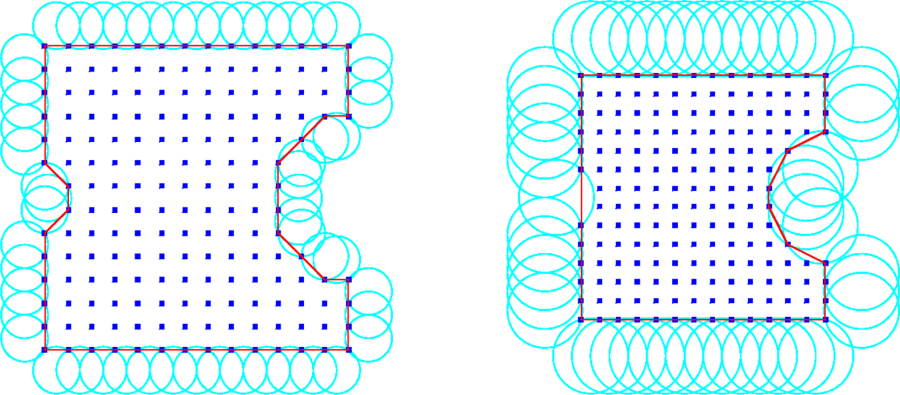
\includegraphics[width=\textwidth]{alpha_shape2D}
%\label{fig:shape}
%\caption{\textbf{Construction of $\alpha$-shapes.} The boundary of the shape (red line) formed by a set of points (blue dots) in $\mathbb{R}^2$ is detected for $\alpha = 1$ (left) and for $\alpha=2$ (right) \cite{sabel2017application}.}
%\label{fig:shape2d}
%\end{center}
%\end{figure}
Straightening the arcs to line segments we obtain broken lines which constitute the boundary of the so-called $\alpha$-shape of the point set $\mbox{\insieme{U}}$. 
A very small spoon will allow us to eat the entire ice cream without eating any piece of chocolate, while with a larger spoon we are not able to eat any chunk of the ice cream without chocolate pieces. In this example, the chocolates pieces are the points of set $\mbox{\insieme{U}}$ and, the parameter $\alpha$ determines the radius of the carving spoon (the spherical spoon in two-dimension is simply a circle).\\ \indent 
The formal definition of $\alpha$-shape was first given by Edelsbrunner, Kirkpatrick and Seidel in 1983 \cite{edelsbrunner1983shape}. They describe $\alpha$-shape as a generalization of the convex hull of a finite set of points in the plane. Let $\alpha$ be a non negative number $0\leq\alpha<\infty$. 
If $\alpha = 0$ the shape degenerates to the point set $\mbox{\insieme{U}}$. On the other hand, when $\alpha\rightarrow\infty$ the $\alpha$-shape is simply the convex hull of \insieme{U}. If $0<\alpha<\infty$ the $\alpha$-shape is a polygon of \insieme{U} \cite{edelsbrunner1994three}. The construction of the $\alpha$-shape is closely related to the Delaunay triangulation of \insieme{U} \cite{mucke1993shapes}. Therefore, a formal definition of triangulation and Delanauy triangulation is now required. \\ \indent
Given a set $\mbox{\insieme{U}}$ of points not all aligned, let us consider the set \insieme{E} of all the straight-line segments whose endpoints are in \insieme{U}. 
A triangulation \insieme{T} of $\mbox{\insieme{U}}$ is the subset of \insieme{E} with the maximum number of segments such that all the line segments of \insieme{T} intersect only at their endpoints \cite{lloyd1977triangulations}. 
\\ \indent Before giving a more formal definition of triangulation, let us define a partition of a set $\mbox{\insieme{X}}\subset \mathbb{R}^2$ as a collection of the subsets which divide \insieme{X} into non-overlapping regions so that any point in \insieme{X} is located in only one region. 
\begin{definition} \indent Let $\mbox{\insieme{P}}\subset \mathbb{R}^2$ be the convex hull of $\mbox{\insieme{U}}$ and $\mbox{\insieme{T}} = \{\mbox{\insieme{T}}_1, \cdots, \mbox{\insieme{T}}_\variabile{h}\}$ be a partition of $\mbox{\insieme{P}}$ into closed triangles, that is triangles that include their edges. Suppose that the following properties hold:
\begin{itemize}
\item[a)] $\mbox{\insieme{P}} = \bigcup_{\variabile{i} = 1}^{\variabile{h}}\mbox{\insieme{T}}_\variabile{i}$,
\item[b)] $\forall \mbox{ \insieme{T}}_\variabile{i}, \mbox{\insieme{T}}_\variabile{j} \in \mbox{\insieme{T}}$, $\mbox{\insieme{T}}_\variabile{i} \neq \mbox{\insieme{T}}_\variabile{j}$, and 
\begin{equation*}
\textrm{int}(\mbox{\insieme{T}}_\variabile{i})\cap \textrm{int}(\mbox{\insieme{T}}_\variabile{j}) = \emptyset,
\end{equation*}
where $\textrm{int}(\mbox{\insieme{T}}) = \mbox{\insieme{T}}-\partial \mbox{\insieme{T}}$,
\end{itemize}
then $\mbox{\insieme{T}}$ is called a \textit{triangulation} of $\mbox{\insieme{P}}$ \cite{Numericalmethods}.
\end{definition}
The Delaunay triangulation $\mbox{\insieme{T}}^{\prime}$ of the point set \insieme{U} has the property that the circumcircle of any triangle of $\mbox{\insieme{T}}^{\prime}$ does not contain any point of \insieme{U}. This is called the Delaunay property. Next, a very commonly used algorithm to construct such triangulation is explained.\\ \indent 
$\mbox{\insieme{T}}^\prime$ is constructed by modifying a general triangulation \insieme{T} such that every point satisfies the Delaunay property. 
Therefore, every triangle that does not satisfy such property is flipped such that the new edge is part of the triangulation, see Figure \ref{fig:Delaunay}. 
Given, for example, an arbitrary triangulation \insieme{T} in two-dimensions, for each edge $\overline{\point{ab}}$ in \insieme{T} which is not on the boundary of the convex hull the two triangles 
$\Delta_{\point{abc}}$ and $\Delta_{\point{abd}}$ with the common edge $\overline{\point{ab}}$ are identified. Then, if either the circumcircle of triangle $\Delta_{\point{abc}}$ contains point \point{d} or the circumcircle of triangle $\Delta_{\point{abd}}$ contains point \point{c}, the edge $\overline{\point{ab}}$ cannot be included in the Delaunay triangulation and, therefore, $\overline{\point{ab}}$ is replaced by the edge $\overline{\point{cd}}$ such that the triangles $\Delta_{\point{acd}}$ and $\Delta_{\point{bcd}}$ are constructed. The new edge $\overline{\point{cd}}$ locally satisfies the Delaunay property and the triangles $\Delta_{\point{acd}}$ and  $\Delta_{\point{bcd}}$ are added to the Delaunay triangulation $\mbox{\insieme{T}}^\prime$.  
\begin{figure}[t]\label{fig:Delaunay}
\begin{subfigure}[t]{0.48\textwidth}
\centering
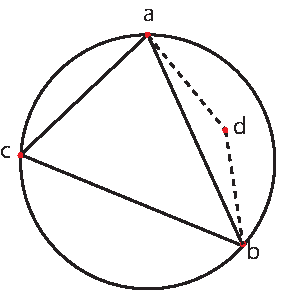
\includegraphics[]{triangle_alpha_shapes}
\label{fig:shape}
\caption{\textbf{Not acceptable triangle.} The point \point{d} is inside the circle circumscribing the triangle $\Delta_{\point{abc}}$, therefore the edge $\overline{\point{ab}}$ cannot be included in the Delaunay triangulation.}
\end{subfigure}
\hfill
\begin{subfigure}[t]{0.48\textwidth}
\centering
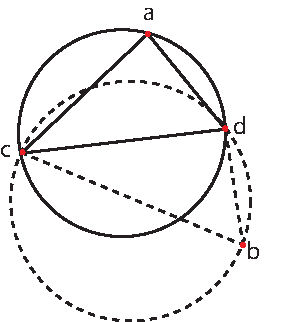
\includegraphics[]{triangle_alpha_shapes_flipped}
\caption{\textbf{Acceptable triangle.} The flipped triangle $\Delta_{\point{acd}}$ satisfies the Delaunay property, thus it is included in the Delaunay triangulation.}
\end{subfigure}
\caption{Construction of the Delaunay triangulation in 2D.}
\label{fig:Delaunay}
\end{figure}
\\ \indent Several other algorithms have been developed to construct a Delaunay triangulation, see for example \cite{lee1980two, renka1997algorithm}.
 Given a point set $\mbox{\insieme{U}}$ and a triangulation \insieme{T}, it can be proved that the corresponding Delaunay triangulation $\mbox{\insieme{T}}^\prime$ is unique. Moreover, it maximizes the largest minimum angle among all possible triangulations of a point set $\mbox{\insieme{U}}$ \cite{press2007numerical}.
\\ \indent Alternatively, the Delaunay triangulation can be constructed as the dual of the Voronoi diagram \cite{fortune1992voronoi}. Let $\mbox{\insieme{X}}\subset\mathbb{R}^2$ be a metric space endowed with the Euclidean distance $d(\point{x}, \point{y})$ for $\point{x}, \point{y}\in \mbox{\insieme{X}}$. For \textit{almost}\footnote{Note the importance of the word \textit{almost}. Some points can have the same distance with two or more points of $\mbox{\insieme{U}}$.} every point $\point{x}\in \mathbb{R}^2$, there is a unique point that is the closest point to $\point{x}$. The Voronoi cell of a point $\point{u}_\variabile{i}\in \mbox{\insieme{U}}$ contains all points in $\mathbb{R}^2$ that are closest to $\point{u}_{\variabile{i}}$, see Figure \ref{fig:Voronoi}. The Voronoi diagram of $\mbox{\insieme{U}}\subset \mathbb{R}^2$ is defined as the set of all Voronoi cells \cite{cazals2005conformal}. A more formal definition of the Voronoi diagram is given in the following.
\begin{defn}
Let $\mbox{\insieme{U}}=\{\point{u}_1,\cdots,\point{u}_N\}$ be a set of points in $\mathbb{R}^2$. The Voronoi cell $\mbox{\insieme{V}}_\variabile{i}$ associated to point $\point{u}_\variabile{i}$ is defined as:
\begin{equation}
\mbox{\insieme{V}}_\variabile{i}=\{\point{x}\in \mathbb{R}^2\; | \;|\point{x}-\point{u}_\variabile{i}|<|\point{x}-\point{u}_\variabile{j}| \quad \forall \variabile{j}\neq \variabile{i} \}.
\end{equation}
The Voronoi diagram $\mbox{\insieme{V}}$ is defined as 
\begin{equation}
\mbox{\insieme{V}} = \bigcup_{\variabile{i}=1}^N \mbox{\insieme{V}}_\variabile{i}
\end{equation}
 where $\mbox{\insieme{V}}_{\variabile{i}}\cap \mbox{\insieme{V}}_{\variabile{j}}= \emptyset$ for $\variabile{i}\neq\variabile{j}$.
\end{defn}
For the definition of Voronoi diagram in higher dimensions see \cite{brown1979voronoi}.
\begin{figure}[t]
\centering
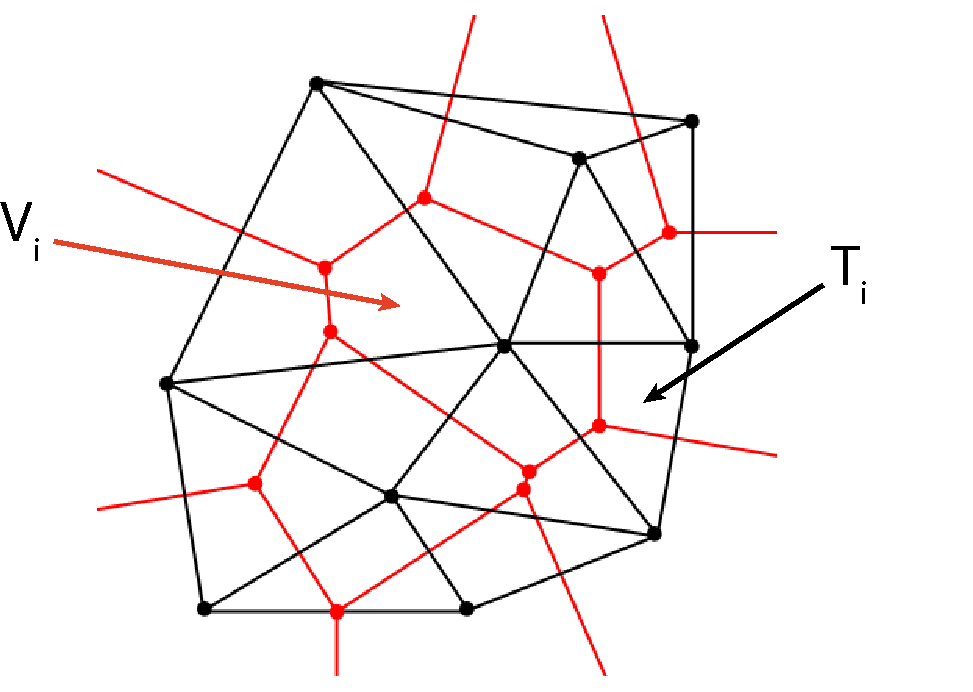
\includegraphics[width = 0.7 \textwidth]{Delanay_Voronoi1}
\caption{\textbf{Relationship between the Delaunay triangulation and the Voronoi Diagram \cite{Wiki4}.} The black line segments are the boundaries of the Delaunay triangulation, the red line segments constitutes the boundaries of the Voronoi diagram.}
\label{fig:Voronoi}
\end{figure}
\\ \indent The Delaunay triangulation triangulates the convex hull of \insieme{U} and, therefore it does not constitute a suitable method for reconstructing the contour formed by a point cloud. The $\alpha$-shape method was developed to solve such problem \cite{edelsbrunner2010alpha, guo1997surface}. Starting from the Delaunay triangulation $\mbox{\insieme{T}}^\prime$ of a point set \insieme{U}, the corresponding $\alpha$-shape of $V$ is formed by the only triangles of $\mbox{\insieme{T}}^\prime$ that satisfy the so-called "$\alpha$-test" which is briefly explained.
For each triangle, we calculate the circumradius, i.e., the radius of the circumcircle. If this radius is larger than $\alpha$ the triangle is removed from the shape. The choice of the parameter $\alpha$ is highly significant in the $\alpha$-shapes procedure and, it has to be selected such that the desired approximation of the shape formed by the points of $V$ is obtained.\\ \indent
%Therefore, $\alpha$ is closely related to the radius of the circumcircles. A possible strategy is to find the radius of the greater empty circumcircle. Thus $\alpha$ can be selected according to the density $\delta$ of the point sets $V$
%with $C$ a constant and $\delta$:
%\begin{equation}
%\delta=\frac{N}{A}\; ,
%\end{equation}
%where $N$ is the number of points in $V$ and $A$ is the area of the convex hull of $V$.
%%Note that, if we scale the dimensions of the  
%The value of $\alpha$ can be chosen, for instance, inversely proportional to $\sqrt{\delta}$:
%\begin{equation}
%\alpha=C\frac{1}{\sqrt{\delta}}\;,
%\end{equation}
%Note that, while $\delta$ is given for a fixed point set $V$, the value of $C$ needs to be determined by numerical simulations.\\ \indent 
To summarize, the $\alpha$-shape construction can be outlined as follows:
\begin{enumerate}
\item Construct a Delaunay triangulation\footnote{In the simulations we present in this chapter the Matlab function \textit{Delaunay} is used \cite{matlab_delaunay}.} $\mbox{\insieme{T}}^\prime$ of the point cloud $\mbox{\insieme{U}}$;
\item For every triangle $\mbox{\insieme{T}}^\prime(i)\in \mbox{\insieme{T}}^\prime$ calculate its circumradius $r(i)$;
\item If $r(i)\leq\alpha$ keep the triangle $\mbox{\insieme{T}}^\prime(i)$ in the triangulation;
\item If $r(i)>\alpha$ remove the triangle from the triangulation;
\item Select from the new triangulation obtained those sides that belong to only one triangle, the so-called \textit{free boundary edges}\footnote{In the simulations we present in this chapter the Matlab function \textit{freeBoundary} is used \cite{matlab_free}.}. By definition, the free boundary edges are not a common edge of any two triangles.
\end{enumerate}
%% Insert algorithm
%\begin{algorithm}[h]
%\caption{$\alpha$-shape reconstruction}\label{alg:alphashapes}
%\begin{algorithmic}[1]
%\Procedure{$\alpha$-shape}{$V$, $\alpha$}
%\State Construct a Delaunay triangulation of the point cloud $V$
%\State$T^\prime\gets$ all triangles of the Delaunay triangulation
%\State For every 
%\State Calculates the radius of the circle circumscribed by the vertices of every triangle
%\State $r(i) \gets$
%\State For {every triangle in $T^\prime$}
%\State $(\variabile{q}_1^4, \variabile{p}_1^4) \gets \mbox{left and upper corner of source PS: (-\variabile{a}, 1)} $
%\For{$ \variabile{k}= 1 \to 4 $}
%\State Trace the ray with initial coordinates $(\variabile{q}_1^\variabile{k}, \variabile{p}_1^{\variabile{k}})$ in \set{S}{}{};
%\State Calculate the corresponding path $\Pi^{\variabile{k}}$;
%\State $\mbox{Ray}.\variabile{q}\gets [\mbox{Ray}.\variabile{q}, \variabile{q}_1^\variabile{k}]$;
%\State $\mbox{Ray}.\variabile{p}\gets [\mbox{Ray}.\variabile{p}, \variabile{p}_1^\variabile{k}]$;
%\State Store the corresponding path $\Pi^{\variabile{k}}$.
%\State $\mbox{Ray}.\Pi\gets [\mbox{Ray}.\Pi, \Pi^{\variabile{k}}]$;
%\EndFor
%\State VL $\gets [1, 2, 4]$ \Comment{VL = vertices of the left triangle}
%\State VR $\gets [2,3, 4]$   \Comment{VR = vertices of the right triangle}
%\State \Call{Left Triangle}{VL, Ray, $\varepsilon_{\variabile{q}_1}^{\textrm{min}}, \varepsilon_{\variabile{q}_1}^{\textrm{max}}, \varepsilon_{\variabile{p}_1}^{\textrm{min}}, \varepsilon_{\variabile{p}_1}^{\textrm{max}}$}\Comment{Refine the left triangle} 
%\State \Call{Right Triangle}{VR, Ray, $\varepsilon_{\variabile{q}_1}^{\textrm{min}}, \varepsilon_{\variabile{q}_1}^{\textrm{max}}, \varepsilon_{\variabile{p}_1}^{\textrm{min}}, \varepsilon_{\variabile{p}_1}^{\textrm{max}}$} \Comment{Refine the right triangle} \\
%\Return ;
%\EndProcedure
%\end{algorithmic}
%\end{algorithm}
%\\
%Let us define a Voronoi diagram in a metric space.
%The simplest case that we can have is the two-dimensional case that is the case where $X=\mathbb{R}^2$.
%The tuple $\mathcal{S}=\{1,\cdots,n\}\subset \mathbb{R}^2$ is now a set of points. The Voronoi diagram of $\mathcal{S}$ is a subsection of $\mathbb{R}^2$ such that every other region around a point $p\in \mathcal{S}$ contains all points that are closer to $p$ than to every point in $\mathcal{S}$. A triangulation of the point set $\mathcal{S}$ is a set of edges $\mathcal{E}$ whose extremes are points of $\mathcal{S}$ such that the faces of each triangle are bounded by three edges and any edge that is not in $\mathcal{E}$ intersects one of the existing edges. The Delaunay triangulation is the dual graph of the Voronoi diagram: it consists of vertices (the points in $\mathcal{S}$) and it has an edge between two vertices if the two corresponding faces share an edge. 
$\alpha$-shapes provide a nice mathematical definition of the \textit{shape} of
a set of points. In two dimensions, $\alpha$-shapes gives the contour of the point cloud which is approximated by a family of line segments. 
Although they are a powerful tool for determining the shape of a point cloud, there exist shapes that are not described well by classical $ \alpha $-shapes. Indeed, for some point sets there is no value of $\alpha$ that gives a good approximation of the contour formed by the point cloud. Usually the parameter $\alpha$ is determined according to the density of the point cloud, therefore, it can be difficult to obtain a good approximation of a shape formed by a non-uniform point set. Furthermore, the $\alpha$-shape method does not work well when the shape we need to approximate has a sharp turn or a joint, this case will be clarified in Section \ref{sec:results-Tir-alpha} with an example. 
%In this case $\alpha$-shapes often give a "webbed-foot" appearance at such joints since they improperly connect the adjacent surfaces. 
\\ \indent There are several ways to determine the value of $\alpha$ \cite{mandal1997selection}; in the next section we provide a technique that exploits the conservation of \'{e}tendue in PS. 
%The first step of this method is to make a triangulation of the point cloud.
%Then the key idea is to compute somehow the point-density of each point and use this to get an approximation of the point density of a triangle. In this way one can reduce the $\alpha$-value in areas where the triangle's point density (see Equation \ref{delta_t} for the definition) is higher than average in such a way that is possible to obtain a finer level of detail for areas that have an higher density.
%More precisely, each point $ \textbf{p}\in \mathcal{S} $ has a local point density defined as
%\begin{equation}
%\delta (\textbf{p})= \sum_{\textbf{q}\in \mathcal{S}}\Big( 1-\frac{\textrm{d}(q,p)}{\lambda}\Big) \qquad \forall \textbf{q} \mbox{\;\;such that\;\;} \textrm{d}(\textbf{p},\textbf{q})<\lambda\,,
%\end{equation}
%where $ \lambda $ is the constant radius of the local neighborhood and $\textrm{d}(\textbf{x},\textbf{y})$ is the Euclidean distance.
%When local density is larger than the average, that is when
%\begin{equation}
%\delta (\textbf{p}) >\frac{1}{| \mathcal{S} |}\sum_{\textbf{q}\in \mathcal{S}}\delta (\textbf{q})
%\end{equation}
%we know some properties about the region surrounding $\textbf{p}$.
%For instance, if the point set is uniformly distributed then it is possible to find areas with a high-density in the case where there are two closely separated surfaces.  In point sets of non-uniform distribution, high densities are found when the surface presents a joint discontinuity. The algorithm developed by Teichmann and Capps is structured as follow.
%After computing density information for each point they make a triangulation of the point set. Then they calculate the average density  $\delta(t)$ for each triangle $\Delta_{abc}$ defined as:
%\begin{equation}
%\delta(t)=\frac{\delta(a)+\delta(b)+\delta(c)}{3 \mu}\,,
%\label{delta_t}
%\end{equation}
%where $\mu$ is the global average density of the entire point set $\mathcal{S}$.
%If $\delta(t)$ is greater than $1$ the density of the point cloud is higher. Hence is necessary to define another value of $\alpha$:
%\begin{equation}
%\alpha^{\;\prime} = \frac{\alpha}{\delta(t)^\sigma}
%\end{equation} where $\sigma$ is a value that is adjusted by the user.
%If  $\delta$ is less than $1$ the $\alpha$-value is not modified.
%In this way it is possible to have a finer precision on the shape formed by the point set where the density is higher than the average density. Hence it is possible to distinguish two separated objects with different density.
% We want to determine the boundaries in phase space
% Jorg
% It is useful to understand whether the approximation is correct
\section{Determination of $\alpha$ using \'{e}tendue conservation} \label{sec:Tir_alpha}
As mentioned in Section \ref{sec:PSconcept}, in two-dimensions \'{e}tendue can be seen as an area in PS. 
Therefore, given an optical system with a source $\point{S} = [-\variabile{a}, \variabile{a}]$, the \'{e}tendue at the source coincides with the area of source PS, and it is given by:
\begin{equation}\label{eq:etenduesource1}
U = 4\n_1 \variabile{a} \sin(\myangle_1^{\textrm{max}})\,,
\end{equation}
 where $\variabile{a}$ is the half length of the source, $\n_1$ the index of refraction of the medium in which the \point{S} is located and $\myangle_1^{\textrm{max}}$ is the maximum value of the angle that the rays make with the normal $\boldsymbol{\nu}_1$ of the source.\\ \indent 
For some optical systems, all the rays emitted by the source arrive at the target, for some others there are also rays that can end at other detectors which are located outside the system. 
Indicating with \set{R}{$1$}{}$(\Pi)$ the regions in source PS formed by the rays that reach the target following path $\Pi$ and with \set{R}{}{}$(\Pi)$ the corresponding regions at the target, the \'{e}tendue $U_1$ at the source restricted to rays that arrive at the target is given by:
\begin{subequations}
\begin{align}
\label{eq:etendueintegralsource}
U\big(\mbox{\set{R}{$1$}{}}(\Pi)\big) = {\int\!\!\int}_{\textup{R}_1(\Pi)} \textrm{d}\variabile{q}\,\textrm{d}\variabile{p}.\\\label{eq:etenduesumsource}
U_1 = \sum_\Pi{U\big(\mbox{\set{R}{$1$}{}}(\Pi)\big)}, 
\end{align}
\end{subequations}
where $U\big(\mbox{\set{R}{$1$}{}}(\Pi)\big)$ is the contribution to the \'{e}tendue given by the rays inside 
\set{R}{$1$}{}$(\Pi)$ in source PS and the sum is over all possible paths $\Pi$ from the source to the target.
Similarly, the \'{e}tendue at the target of the rays emitted by the source is:
\begin{subequations}
\begin{align}
\label{eq:etendueintegraltarget}
U\big(\mbox{\set{R}{}{}}(\Pi)\big) = {\int\!\!\int}_{\textup{R}(\Pi)} \textrm{d}\variabile{q}\,\textrm{d}\variabile{p}.\\ \label{eq:etenduesumtarget}
U_\textrm{t}= \sum_\Pi{U\big(\mbox{\set{R}{}{}}(\Pi)\big)}, 
\end{align}
\end{subequations}
Note that, since both the source and the target are located in air ($\n_1=1$), in (\ref{eq:etendueintegralsource}) and (\ref{eq:etendueintegraltarget}), and from now on, we omit writing the index of refraction $\n_1$.
\\ \indent In order to determine the value of $\alpha$ in the $\alpha$-shape procedure that approximates the boundaries $\partial$\set{R}{}{}$(\Pi)$ accurately, we use \'{e}tendue conservation ($U_{\textrm{t}}= U_1$). The $\alpha$-shapes method is applied to every region \set{R}{}{}$(\Pi)$ for a range of values of $\alpha$;
   for each value an approximation of the boundaries $\partial$\set{R}{}{}$(\Pi)$ is obtained and
   the intersection points $\variabile{q}^{\textrm{\,max}}(\Pi,\variabile{p})$ and $\variabile{q}^{\textrm{\,min}}(\Pi,\variabile{p})$ between $\partial$\set{R}{}{}$(\Pi)$
and the horizontal lines $\variabile{p}=\textrm{const}$, with $\variabile{p}\in[-1,1]$, are computed for every path $\Pi$.
Therefore, Equation (\ref{eq:etendueintegraltarget}) becomes:
\begin{equation}\label{eq:etenduetarg}
 U\big(\mbox{\set{R}{}{}}(\Pi)\big)= \int_{-1}^{1}{\Big(\variabile{q}^{\textrm{\,max}}(\Pi,\variabile{p})-\variabile{q}^{\textrm{\,min}}(\Pi,\variabile{p})\Big)} \,\textrm{d}\variabile{p}.
\end{equation} In case more than two intersection points between the line $\variabile{p}=\textrm{const}$ and $\partial$\set{R}{}{}$(\Pi)$ occur, the previous equation needs to be generalized. Suppose that $\variabile{r}$ intersection points $\big(\variabile{q}^{\,\variabile{i}}(\Pi,\variabile{p}), \variabile{p}\big)_{\variabile{i} = 1, \cdots, \variabile{r}}$ are found. 
Ordering their $\variabile{q}$-coordinates in ascending order, the target \'{e}tendue is calculated by:
\begin{equation}\label{eq:etenduetarg1}
 U\big(\mbox{\set{R}{}{}}(\Pi)\big) = \sum_{\variabile{i} = 1}^{\variabile{m}}\int_{-1}^{1}
{\Big(\variabile{q}^{\,2\variabile{i}}(\Pi,\variabile{p})}-{\variabile{q}^{\,2\variabile{i}-1} (\Pi, \variabile{p}) \Big)}\,\textrm{d}\variabile{p}\,,
\end{equation}
where $\variabile{m}$ is the integer part of $\variabile{r}/2$. 
The integrals in (\ref{eq:etenduetarg}) and (\ref{eq:etenduetarg1}) are calculated discretizing the interval $[-1, 1]$
   into $\nbin=100$ sub-intervals of equal length, the so-called bins, and using the trapezoidal rule.
\\ \indent Matching the \'{e}tendue at the source $U_1$ with the \'{e}tendue at the target $U_{\textrm{t}}$, a unique value $\alpha_{\textrm{c}}$ of $\alpha$ is determined. Implementing the $\alpha$-shapes procedure with $\alpha = \alpha_\textrm{c}$, an approximation of the boundaries $\partial$\set{R}{}{}$(\Pi)$ is found and the intensity at the target can be calculated.\\ \indent If two intersection points between $\variabile{p}=\textrm{const}$ and $\partial$\set{R}{}{}$(\Pi)$ are found the target intensity is calculated using ($\ref{eta2}$). If more than two-intersection points are found we use the generalized equation:
\begin{equation}
I_{\textrm{PS}}(\variabile{p}) = \sum_{\Pi, \variabile{i} }\int_{\variabile{q}^{\,2\variabile{i}-1}(\Pi, \variabile{p})}^{\variabile{q}^{\,2\variabile{i}}( \Pi, \variabile{p})}L(\variabile{q}, \variabile{p})\textrm{d}\variabile{q} =
 \sum_{\Pi, \variabile{i}}\big(\variabile{q}^{\,2\variabile{i}}(\Pi, \variabile{p})-
\variabile{q}^{\,2\variabile{i}-1}( \Pi, \variabile{p})\big)\,,
\label{eq:Ips}
\end{equation}
where $\variabile{q}^{\,2\variabile{i}}( \Pi, \variabile{p})>\variabile{q}^{\,2\variabile{i}-1}( \Pi, \variabile{p})$, the summation over $\Pi$ is for all the paths $\Pi$ for which the intersection $\variabile{p} = \textrm{const}$ and \set{R}{}{}$(\Pi)$ is not empty, and the summation over $\variabile{i}$ is for $\variabile{i} = 1,2, \cdots, \variabile{m}$. The second equation holds as we assume $L(\variabile{q}, \variabile{p})=1$.\\ \indent
To clarify our idea we apply the method to two different optical systems, the results are presented next.
%\\ \indent Let us consider the two-faceted cup introduced in Chapter \ref{chap:raytracing} and depicted in Figure \ref{fig:cup}. The half length of the source is $\variabile{a}=2$, the maximum angle is $\myangle_1^{\textrm{max}} = \pi/2$ and \point{S} is located in air, i.e., $\n_1=1$. Therefore, the total \'{e}tendue is $U=8$. For the two-faceted cup all the rays emitted by \point{S} arrive to \point{T}, hence from \'{e}tendue conservation we obtain that $U_{\textrm{t}} =U_1 = 8$.
%For some optical systems, not all the rays emitted by the source arrive to the target.  
% Explain the idea: use etendue conservation
% Do the example for the two faceted cup
% Explain the TIR collimator
\section{Results for a TIR-collimator}\label{sec:results-Tir-alpha}
We apply the $\alpha$-shapes method to the set of points in target PS obtained by using PS ray tracing.
In this chapter, the procedure is applied to two different kinds of total internal reflection (TIR)-collimators.\\ \indent  
Let us first describe the TIR-collimator depicted in Figure \ref{fig:tir}. It is an optical system symmetric with respect to the $z$-axis, it consists of a lens (central curve), two broken lines adjacent to the lens,
two curved lines on each side and a top formed by a horizontal segment. The lens (line $2$) and the broken lines, formed by a collection of three segments (lines $3, 4, \mbox{ and } 5$ and $9, 10 \mbox{ and } 11$), are refractive line segments while the curved lines (labeled with $6$ and $8$) are designed in such a way that light is totally internal reflected (which explains the name TIR).
The light source $\point{S}$ (line $1$) and the target $\point{T}$ (line $12$) are two straight line segments normal to the optical axis.
The source $\point{S}= [-2,2]$ is located at a height $\variabile{z}_{1} = 0.3$ from the $\variabile{x}$-axis.
 The target $\point{T}= [-9.7, 9.7]$ is parallel to the source and is located at a height $ \variabile{z}= 8.2$. Both \point{S} and \point{T} are located in air ($\n_1=1$).
The volume inside the collimator is filled with a material with index of refraction $\n_2=1.5$ (e.g. glass).
The collimator is surrounded by two vertical lines (lines $13$ and $15$) and two horizontal lines ($12$ and $14$) that receive the light emitted from the source; among these the one at the top (line $12$) is assumed to be the target, and it is located at a small distance from the top (line $7$). 
\begin{figure}[t]
  \begin{center}
  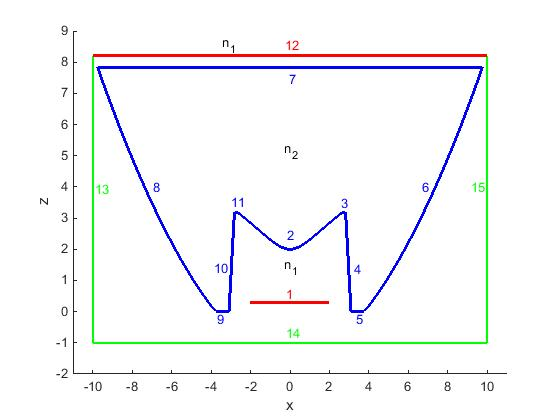
\includegraphics[width=0.7\textwidth]{TIR}
  \end{center}
  \caption{\textbf{Shape of the TIR-collimator.} Each line of the system is labeled with a number.
   The shape of the collimator is shown in blue.
   Three detectors depicted with green lines (surfaces $13$, $14$, and $15$) are located at the left, the right and the bottom of the optical system. The source (line $1$) and the target (line $12$) are depicted in red.}
%The sagitta of the lens is approximately $1.17$.}
  \label{fig:tir}
\end{figure}
\\ \indent
Using PS ray tracing explained in Section \ref{sec:PS_raytracing} with parameters $\varepsilon_{\variabile{q}_1}^{\textrm{max}} = 0.05/4$, $ \varepsilon_{\variabile{p}_1}^\textrm{max} = 0.05/8, $ $\varepsilon_{\variabile{q}_1}^\textrm{min} = 0.8/4$ and $\varepsilon_{\variabile{p}_1}^\textrm{min} = 0.8/8$, around $1.67 \cdot 10^4$ rays are traced (see Table \ref{tab:table}). The rays distribution at the source PS is shown in Figure \ref{fig:sourcePS}, where we depicted the rays that follow the same path with the same color. Seven different paths are found. The yellow rays follow path $\Pi_1 = (1, 2, 7, 12)$; the green rays follow path $\Pi_2 ~= ~(1, 4, 6, 7, 12)$; the red rays follow path $\Pi_3 = (1, 10, 8, 7, 12)$; the magenta rays follow path $\Pi_4= (1, 3, 7, 12)$ and the blue rays follow path $\Pi_5= (1, 11, 7, 12)$. The rays located inside the white areas correspond to rays that do not reach the target, they follow either path $\Pi_6 = (1, 4, 7, 6, 15)$ or path $\Pi_7 = (1,10,7,8,13)$ and they do not give any contribution to the target intensity.
\begin{figure}[t]
\label{fig:sourcePS}
  \begin{center}
  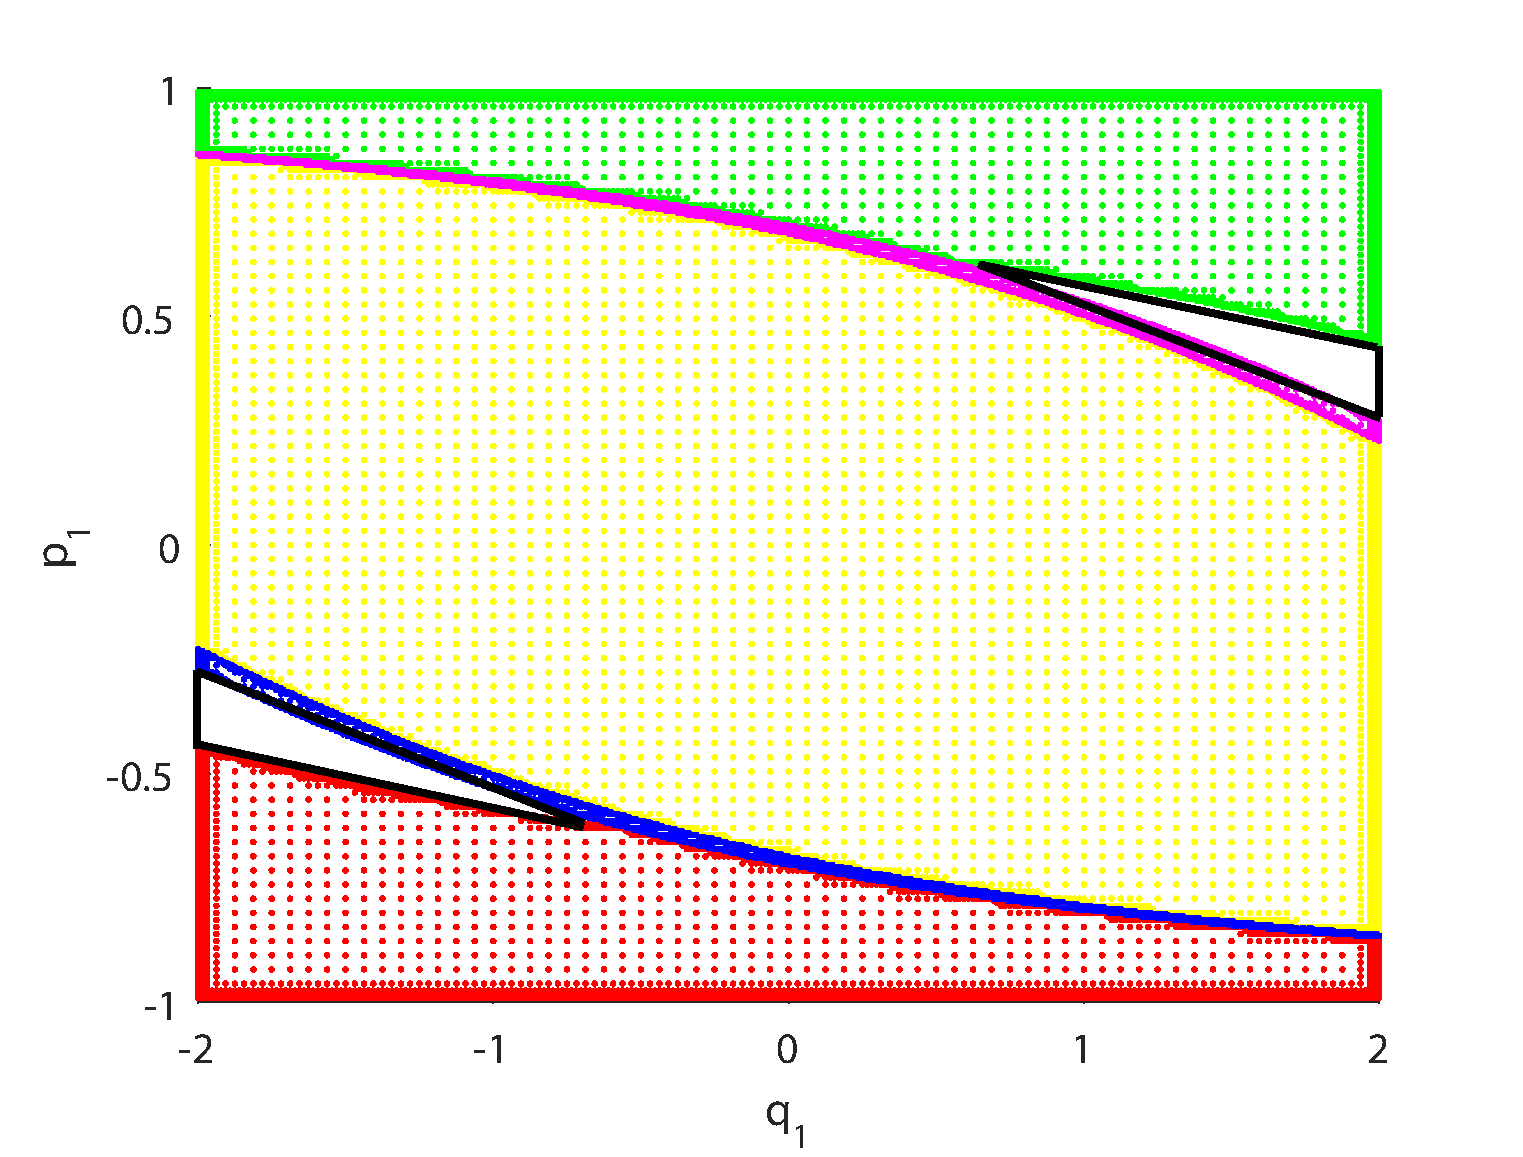
\includegraphics[width=0.8\textwidth]{source1}
  \end{center}
  \caption{\textbf{Distribution of the rays on \point{S}{}{}}. Around $1.67 \cdot 10^4$ rays are traced using the triangulation refinement with parameters:
  $\varepsilon_\variabile{q}^\textrm{max} = 0.8/4 ,$ $ \varepsilon_{\variabile{p}}^\textrm{max} = 0.08/8, $ $\varepsilon_{\variabile{q}}^\textrm{min} = 0.05/4, \varepsilon_\variabile{p}^\textrm{min} = 0.05/8$. Rays that belong to the same region are depicted with the same color. The rays located inside the white areas do not reach the target. The boundaries of the two white regions are approximated by triangles depicted with black lines.}
 \label{fig:sourcePS}
\end{figure}
Note that, given two adjacent paths, the corresponding regions in \set{S}{}{} have usually a common boundary. 
Since for this system not all the rays emitted by the source arrive at the target, $U_{\textrm{t}}$ needs to be compared to the \'{e}tendue $U_1$ at the source given by only those rays that reach the target (the rays that follow paths $\Pi_6$ and 
$\Pi_7$ are discarded). To this purpose, $U_1$ is calculated by removing from the total area $U$ of \set{S}{}{} those areas occupied by the regions formed by the rays that hit the left or the right detector (white regions in Figure $\ref{fig:sourcePS}$).  For the TIR collimator in Figure \ref{fig:tir}, $U$ is obtained from (\ref{eq:etenduesource1}), the source \'{e}tendue $U_1$ corresponding to the area covered by the rays that arrive at the target can be approximated by:
 \begin{equation}\label{eq:Usource}
 U_{1} = U-2A_{T},
 \end{equation}
 where $U=8$ and $A_{T}$ is the approximated area of the white triangles in Figure \ref{fig:sourcePS} surrounded by the black lines.\\ \indent  Next, $U_{\textrm{t}}$ is calculated several times from (\ref{eq:etenduetarg1}) where every time the boundaries $\partial$\set{R}{}{}$(\Pi)$ are obtained by using $\alpha$-shapes for a different value of $\alpha$. 
%An accurate approximation of $\partial$\set{R}{}{}$(\Pi)$ gives a value of $U_{\textrm{t}}$ close to the exact \'{e}tendue. 
%Matching $U_1$ with all the approximations of $U_{\textrm{t}}$ we find the best value $\alpha_c$ of $\alpha$ that approximates $\partial$\set{R}{}{}$(\Pi)$ and, therefore, $U_{\textrm{t}}$. 
\\ \indent To clarify this concept, in Figure \ref{fig:etendueTS} we provide an example where the source \'{e}tendue $U_1$ and target \'{e}tendue $U_{\textrm{t}}$ are computed from a set of around $1.67\cdot 10^4$ rays. The approximated source \'{e}tendue $U_1\approx 7.77$ is depicted with the red line. The blue line shows how the \'{e}tendue at the target changes as a function of $\alpha$. The smallest difference $\Delta U = |U_1-U_{\textrm{t}}|$ is obtained using $\alpha = \alpha_\textrm{c} = 0.08$.
 \begin{figure}[t]
  \begin{center}
  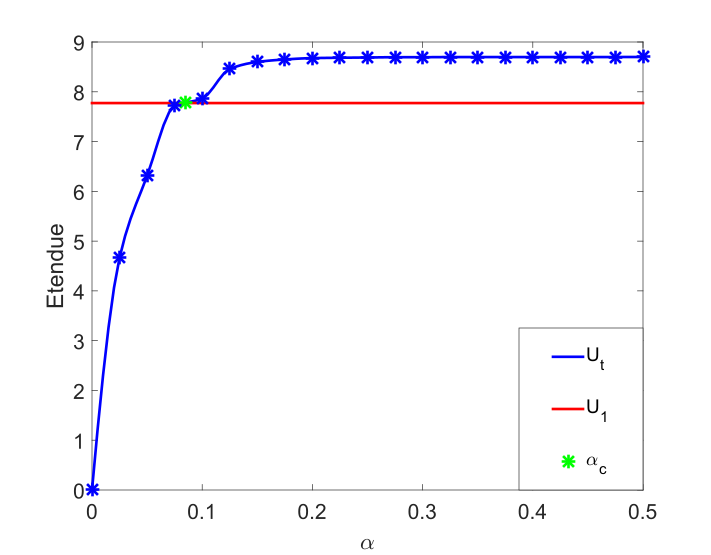
\includegraphics[width=0.7 \textwidth]{etendue_alpha_shapes}
  \end{center}
  \caption{\textbf{Etendue for the TIR-collimator.} $U_\textrm{t}$ is computed for a range of values of $\alpha$. $U_1 \approx 7.77$. The green dot indicates the value of $\alpha_\textrm{c} = 0.08$ which gives a good approximation of the boundaries $\partial$\set{R}{}{}$(\Pi)$ at the target.
   Around $1.67 \cdot 10^4$ rays have been traced using PS ray tracing.
  }
  \label{fig:etendueTS}
\end{figure}
In Figure \ref{fig:targetPS} we show the boundaries 
$\partial$\set{R}{}{}$(\Pi)$ in target PS obtained tracing $1.67\cdot10^4$ rays and using $\alpha_\textrm{c}=0.08$.
  \begin{figure}[t]
  \begin{center}
  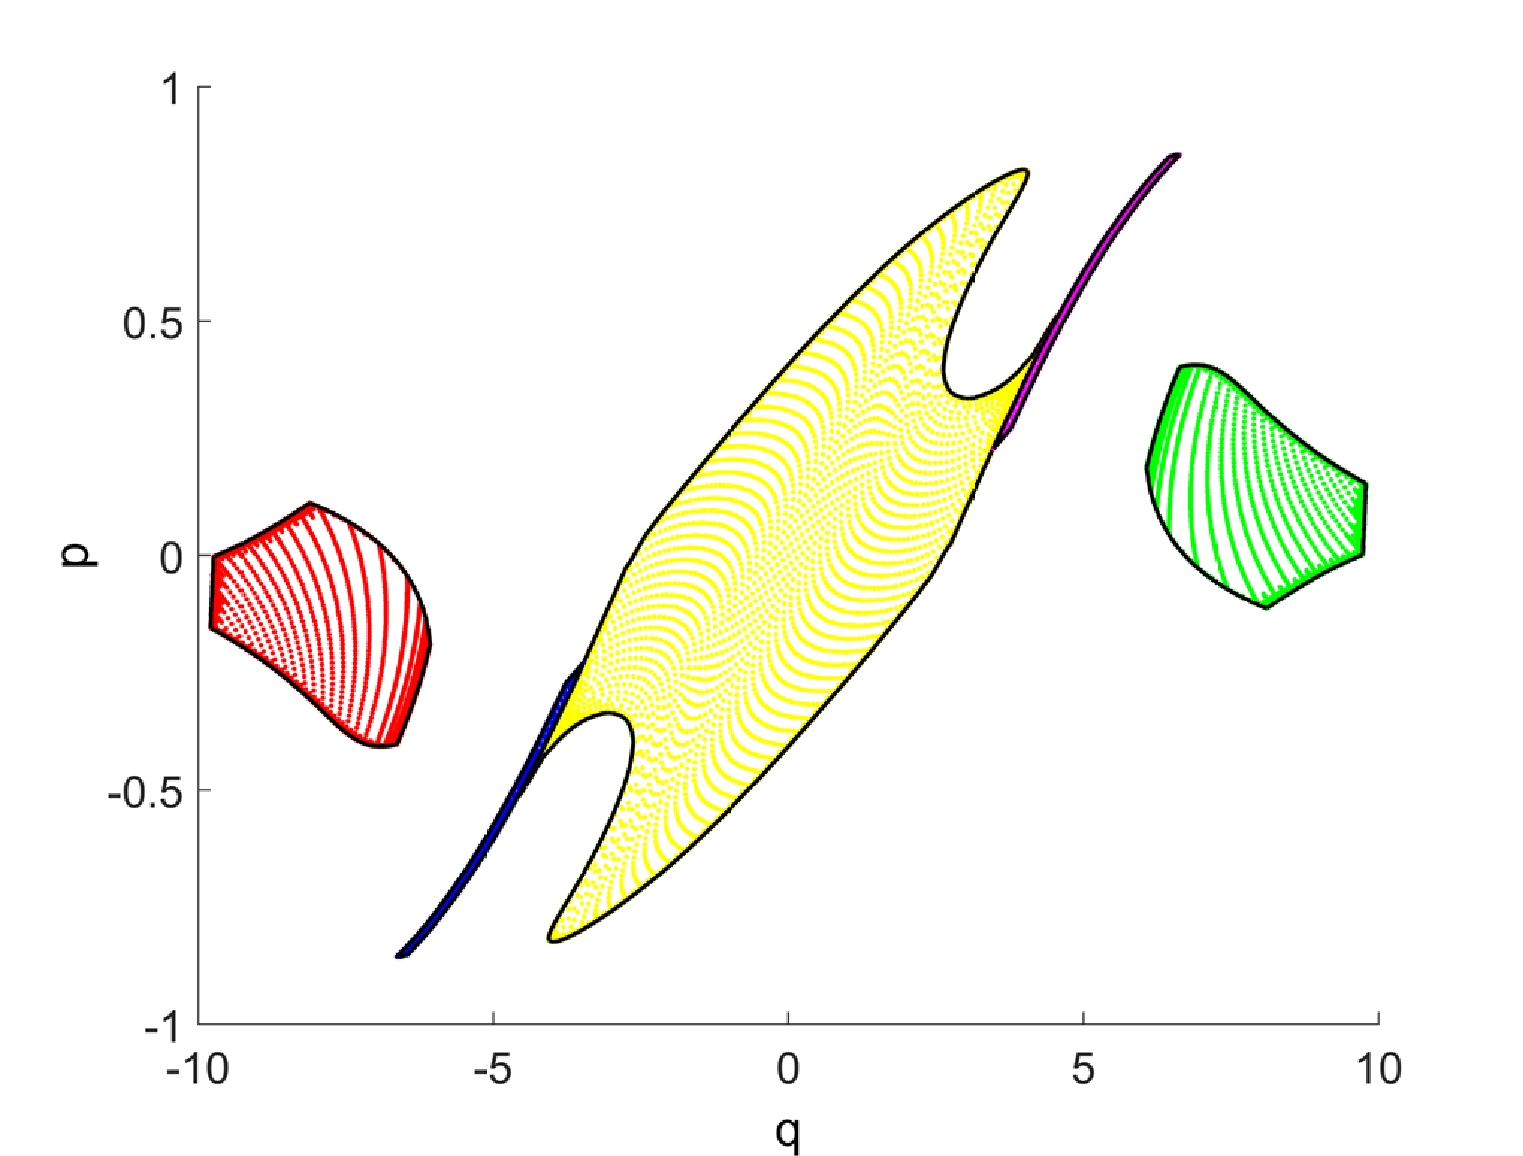
\includegraphics[width=0.7\textwidth]{target_alpha_shapes}
  \end{center}
  \caption{\textbf{Target PS representation.} A set of $1.67 \cdot 10^4$ rays are traced.
  Rays that follow the same path are depicted with the same color. The choice of the colors is consistent with Figure $\ref{fig:sourcePS}$. The boundaries $\partial$\set{R}{}{}$(\Pi)$ are computed through the $\alpha$-shapes method with $\alpha = \alpha_\textrm{c} = 0.08$.}
  \label{fig:targetPS}
\end{figure}
The target intensity $I_{\textrm{PS}}(\variabile{p})$ for $\variabile{p}\in[-1,1]$ is obtained from Equation (\ref{eta2}). \\ \indent
To validate our method we compare the PS intensity with the QMC intensity. 
To this purpose a partitioning $P_2:-1=\variabile{p}_{0}<\variabile{p}_1<\cdots<\variabile{p}_{\nbin}=1$ of the interval $[-1,1]$ into $\nbin=100$ bins is considered. 
The averaged and normalized PS intensity $\hat{I}_{\textrm{PS}}$ is calculated for every 
$\big(\variabile{p}^{\variabile{h}+1/2} = \frac{1}{2}(\variabile{p}^{\variabile{h}+1}+ \variabile{p}^{\variabile{h}})\big)_{\variabile{h}=0, \cdots, \nbin-1}$ dividing the PS averaged intensity by the total \'{e}tendue:
\begin{equation}\label{eq:normalized_PS_intensity}
\hat{I}_{\textrm{PS}}(\variabile{p}^{\variabile{h}+1/2}) = \frac{1}{U_{\textrm{t}}}\int_{\variabile{p}_{\variabile{h}}}^{\variabile{p}_{\variabile{h}+1}} I_{\textrm{PS}}(\variabile{p})\textrm{d}\variabile{p}.
\end{equation}
The averaged and normalized QMC intensity $\big(\hat{I}_{\textrm{QMC}}(\variabile{p}^{\variabile{h}+1/2})\big)_{\variabile{h} = 0, \cdots, \nbin-1}$ is given by
\begin{equation}\label{eq:normalized_MC_intensity}
\hat{I}_{\textrm{QMC}}(\variabile{p}^{\variabile{h}+1/2}) = \frac{\nrays[\variabile{p}^{\variabile{h}},\variabile{p}^{\variabile{h}+1})}{\nrays[-1,1)} 
\qquad \mbox{ for } \variabile{p}\in[\variabile{p}^{\variabile{h}}, \variabile{p}^{\variabile{h}+1}).
\end{equation} 
Both approximate intensities $\hat{I}_{\textrm{A}} (\textrm{A} = \textrm{PS}, \textrm{QMC})$ are compared to an intensity $\hat{I}_{\textrm{ref}}$ taken as a reference. 

For some optical systems, there is an explicit solution for the target intensity, but this is not the case of the TIR-collimator.
Therefore, a QMC simulation with $10^7$ rays is used to obtain the averaged normalized intensity $\hat{I}_{\textrm{ref}}$.
The intensity profile $\hat{I}_{\textrm{PS}}
$ obtained using PS ray tracing with $8.3\cdot 10^4$ rays and $\alpha= \alpha_\textrm{c} = 0.06$ is depicted in Figure \ref{fig:intensityMCPS} with a red line.
$\hat{I}_{\textrm{PS}}$ is hardly distinguishable from $\hat{I}_{\textrm{ref}}$ which is indicated with the dashed and blue line in Figure $\ref{fig:intensityMCPS}$.\\ \indent
  \begin{figure}[h]
    \centering
    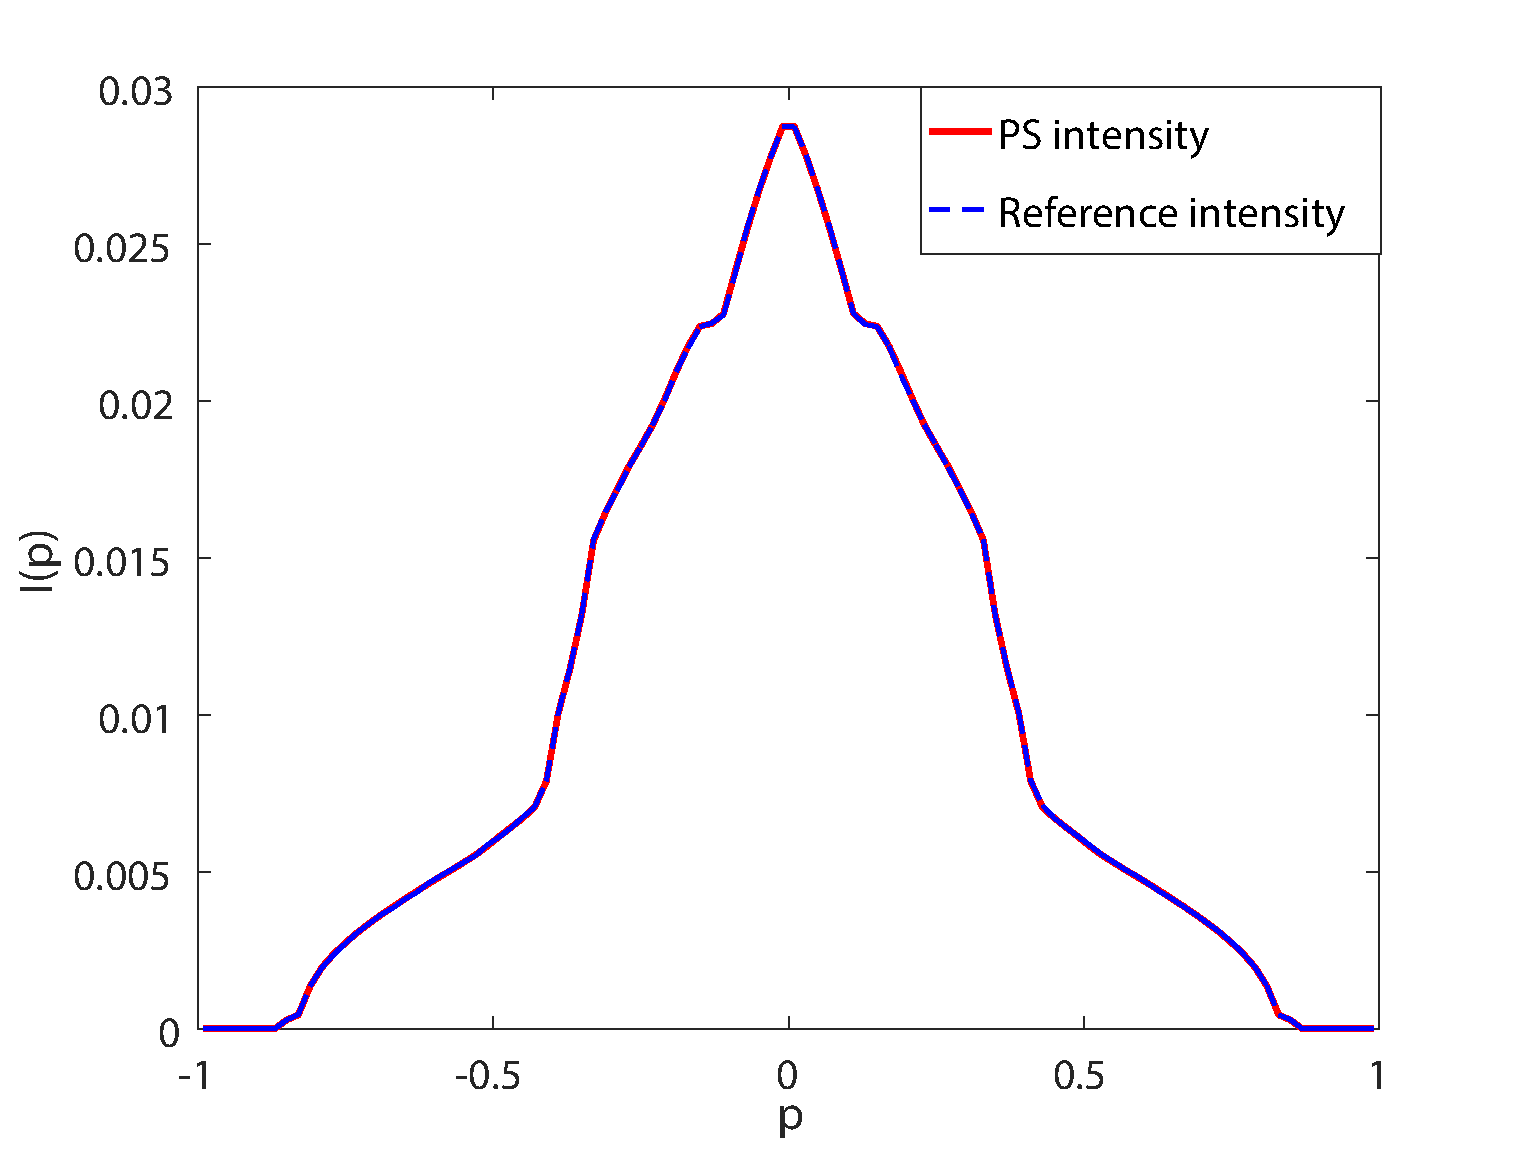
\includegraphics[width=0.7\textwidth]{intensity_alpha_shapes}
\caption{\textbf{Target intensity profile.}
The exact intensity is computed using the QMC method for a set of $10^7$ rays. For the PS intensity a set of $8.3\cdot 10^4$
rays is considered and $\alpha_\textrm{c} = 0.06$ is chosen to compute the boundaries $\partial$\set{R}{}{}$(\Pi)$.}
  \label{fig:intensityMCPS}
\end{figure}
Finally, we calculate the error between $\hat{I}_{\textrm{A}}$ and $\hat{I}_{\textrm{ref}}$, defined as:
\begin{equation}\label{eq:error}
\mbox{error} = \frac{\sum_{\variabile{h}= 1}^{\nbin}| \hat{I}_{\textrm{A}}(\variabile{p}^{\variabile{h}+1/2}) - \hat{I}_{\textrm{ref}}(\variabile{p}^{\variabile{h}+1/2})|}{\nbin}.
\end{equation}
The QMC and PS intensities are calculated several times increasing the number of rays to improve the accuracy.
Table \ref{tab:table} and \ref{tab:table2} describe how the number of rays traced affects the error. 
In Table \ref{tab:table} the correlation between $\alpha_\textrm{c}$ and the number of rays is evident.
%determined by the values of $\varepsilon^{\textrm{min}}_\variabile{p}$, $\varepsilon^{\textrm{min}}_{\variabile{q}}$, 
%$\varepsilon^{\textrm{max}}_{\variabile{p}}$ and $\varepsilon^{\textrm{max}}_{\variabile{q}}$. 
Note that increasing the number of rays the value of $\alpha_\textrm{c}$ and the corresponding error decrease. 
\begin{table}[htbp] \label{tab:table}
\centering
\caption{\bf Errors of the PS intensity}
\begin{tabular}{lllllll}
 \hline  Number \\ of rays\;  & $\varepsilon^{\textrm{max}}_{\variabile{q}} $  & $\varepsilon^{\textrm{min}}_{\variabile{q}} $   \;     & $\varepsilon^{\textrm{max}}_{\variabile{p}}$\;
  & $\varepsilon^{\textrm{min}}_\variabile{p}$\; & $\alpha_\textrm{c}$  & PS error \\
  \hline 
 $3\,339$ & $0.8$  & $0.05$  & $0.8/2$  & $0.05/2$ & $0.14$ & $1.47\cdot10^{-3}$ \\
$7\,567$  & $0.8/2$  & $0.05/2$  & $0.8/4$  & $0.05/4$ & $0.10$ & $3.01\cdot 10^{-4}$  \\
$16\,755$  & $0.8/4$  & $0.05/4$  & $0.8/8$  & $0.05/8$ & $0.08$ & $8.60\cdot 10^{-5}$ \\
 $83\,005$ & $0.8/16$  & $0.05/16$  & $0.8/32$  & $0.05/32$ & $0.06$ & $1.31\cdot 10^{-5}$ \\
 \hline
 \end{tabular}
 \label{tab:table}
 \end{table}
\\ \indent In Table \ref{tab:table2} the numerical results of QMC ray tracing are reported.
Increasing the number of rays traced, the error gradually decreases.
\begin{table}[htbp]
\centering
\caption{\bf Error of the QMC intensity}
\begin{tabular}{ll} \hline   Number of rays\; & QMC error\\
 \hline $10^3$  & $1.65\cdot10^{-3}$ \\
$10^4$  & $3.96\cdot 10^{-4}$  \\
 $10^5$  & $6.36\cdot 10^{-4}$ \\ 
$10^6$  & $1.02\cdot 10^{-5}$ \\
 \hline
 \end{tabular}
 \label{tab:table2}
 \end{table}
\noindent In Figure $\ref{fig:error}$, the results listed in Table $\ref{tab:table}$ and Table $\ref{tab:table2}$ are shown. The red line depicts the convergence of the PS error and the blue line indicates the QMC error.
\begin{figure}[t]
  \begin{center}
  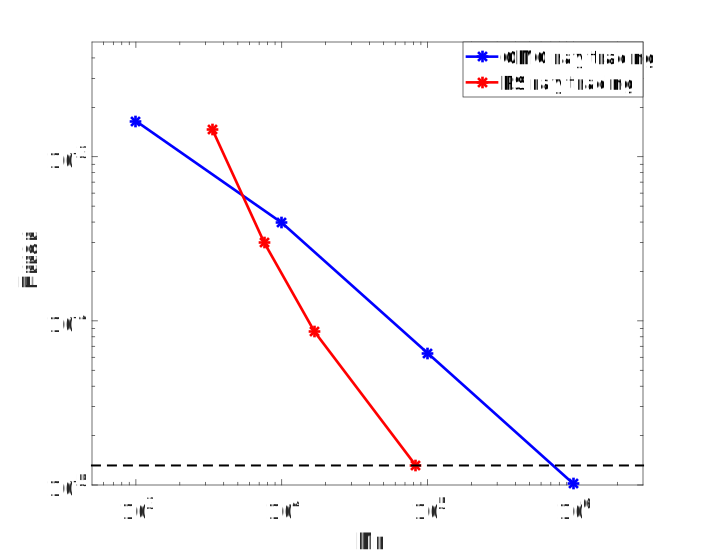
\includegraphics[width=0.7\textwidth]{error_alpha_shapes_vs_qmc_curved}
  \end{center}
  \caption{\textbf{PS and QMC errors as a function of the number of rays}
  The horizontal dotted line shows that an error equal to $1.31\cdot  10^{-5}$ can be obtained tracing almost $10$ times fewer rays in phase space.}
  \label{fig:error}
\end{figure}
%Note from Figure \ref{fig:error} that the error for the QMC method decreases as $\frac{1}{\sqrt{\nrays}}$, while for the PS simulation the speed of convergence is much higher.\\ \indent
We need to emphasize that the convergence of the error of PS ray tracing for increasing $\nrays$ may change according to the design of the optical system.
This is because the approximation of the boundaries in PS depends on the accuracy of the $\alpha$-shapes method.
The $\alpha$-shapes procedure is unable to properly detect the boundaries of regions with a sharp turn if not enough points are given
\cite{teichmann1998surface}. Indeed, on the one hand a low density requires a large value of $\alpha$ to accept the triangles in a region, on the other hand,
 choosing $\alpha$ too large, the shape of the region could be destroyed. Increasing $\alpha$ more triangles are kept and triangles inside the regions \set{R}{}{}$(\Pi)$ could be taken into account creating holes in \set{R}{}{}$(\Pi)$.
\begin{figure}[t]
\centering
\begin{subfigure}{.48\textwidth}
  \centering
  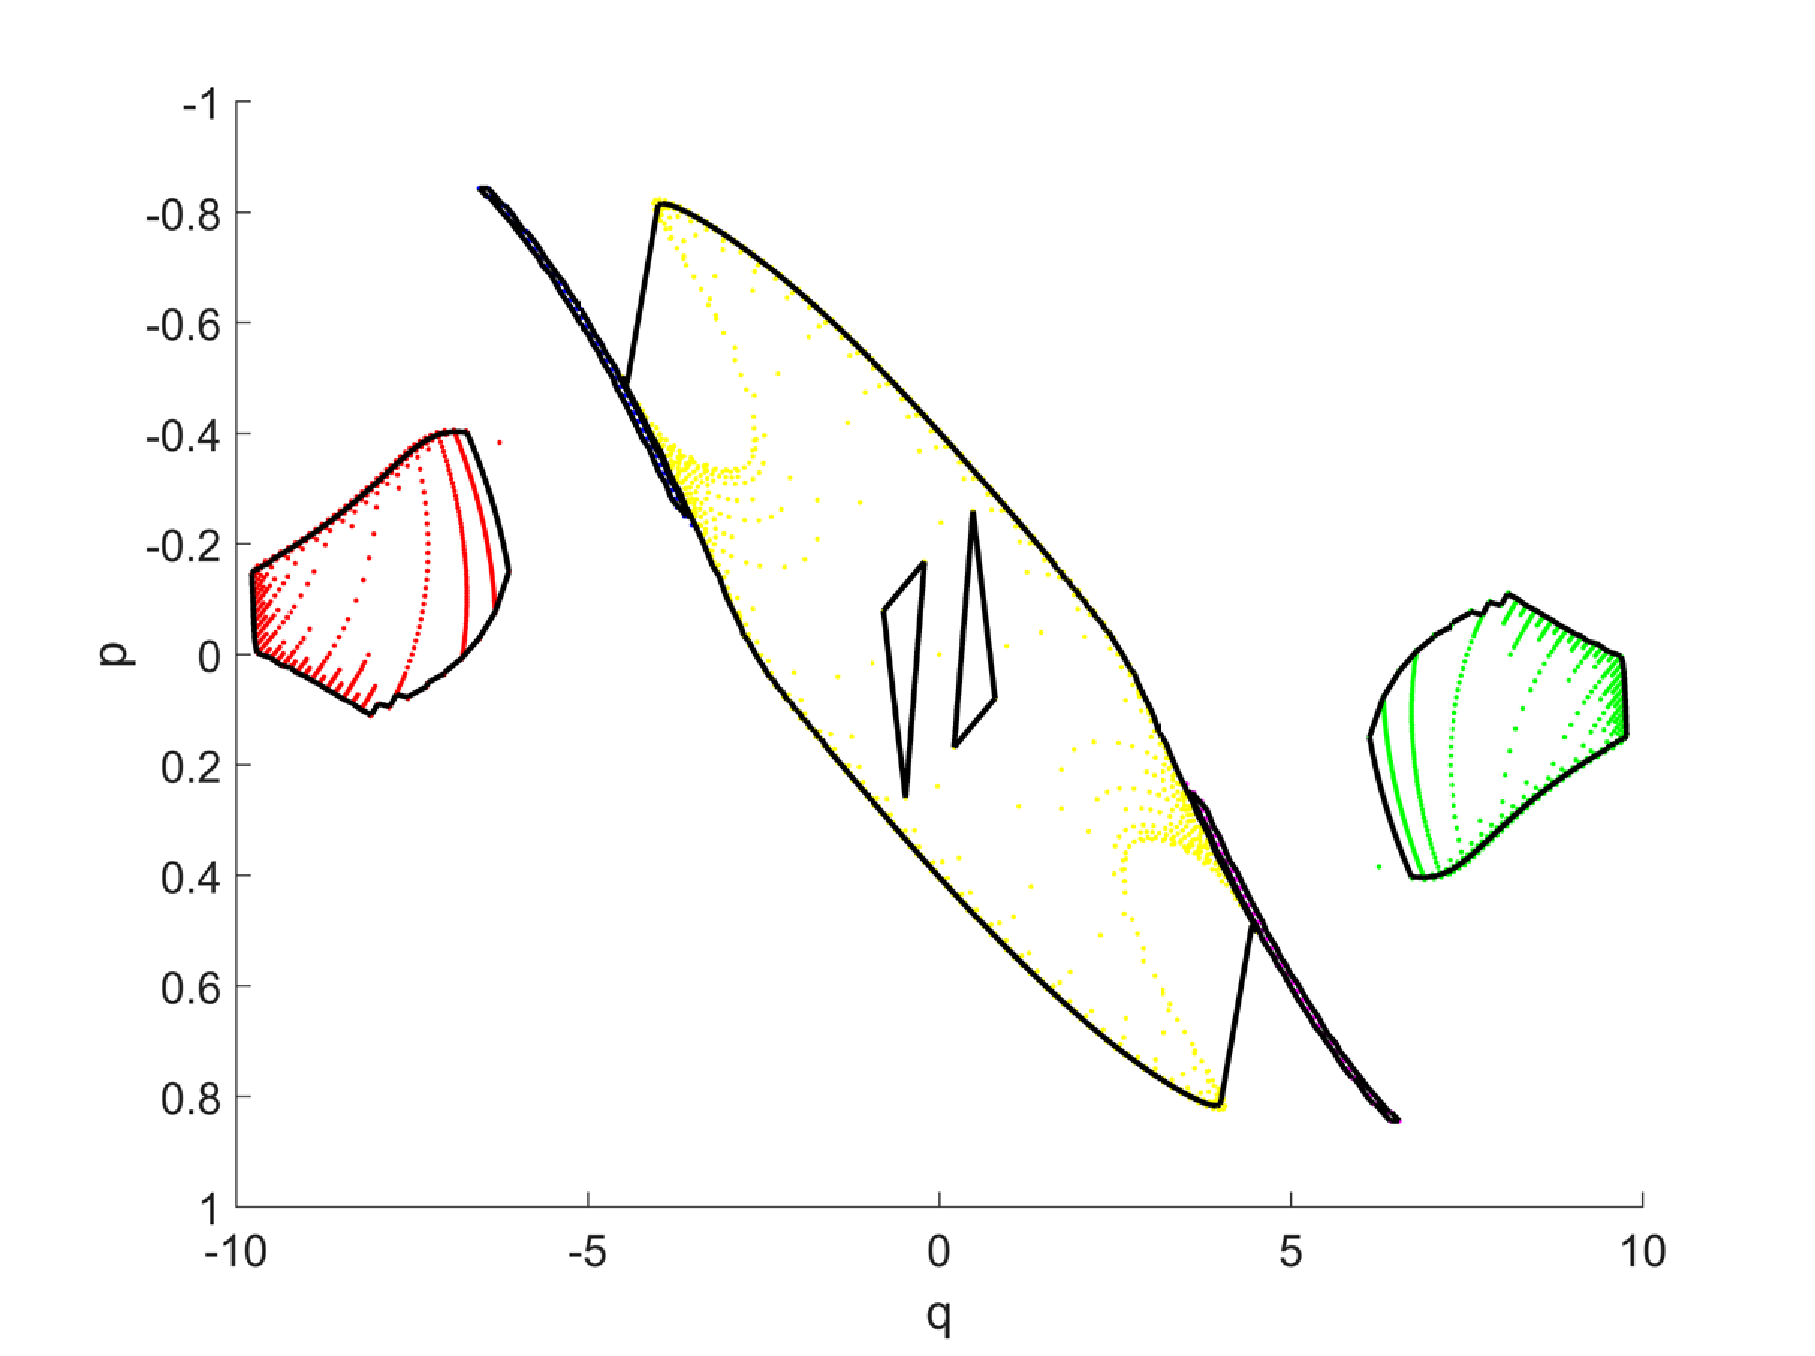
\includegraphics[width=\textwidth]{boundaries_alpha1}
  \caption{Boundaries approximation obtained using the $\alpha$-shapes method with $\alpha_\textrm{c} = 0.3$ (black lines).}
\end{subfigure}
\hfill
\begin{subfigure}{.48\textwidth}
  \centering
  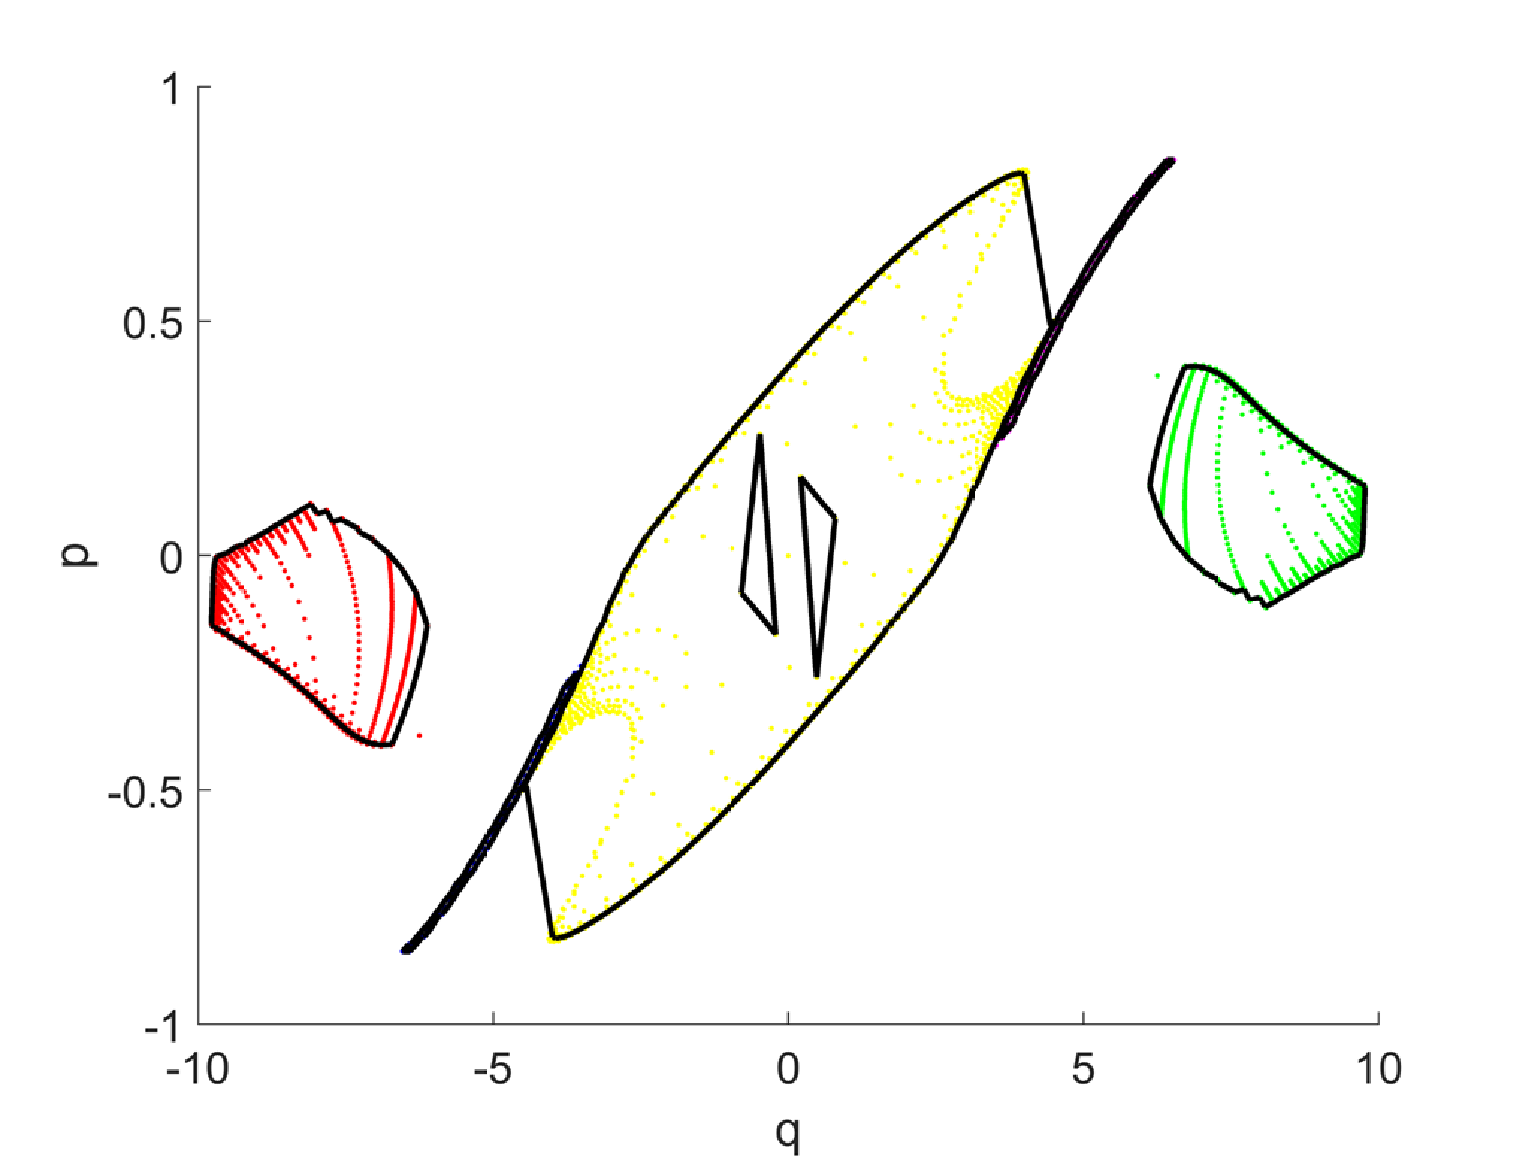
\includegraphics[width=\textwidth]{boundaries_alpha2}
  \caption{Boundaries approximation obtained using the $\alpha$-shapes method with $\alpha_\textrm{c} = 0.31$ (black lines).}
\end{subfigure}
\caption{\textbf{Approximated boundaries at the target PS.} Tracing $3339$ rays and using $\alpha$-shapes, the boundaries cannot be approximated well. 
A small change of the parameter $\alpha$ leads to a completely different approximation of the boundaries.}
\label{fig:Tir1}
\end{figure}
Figure $\ref{fig:Tir1}$ clarifies this concept showing that the region formed by rays that hit the lens is hard to approximate when there is a small number of rays inside the region. Consequently either a region bigger than the area covered by the rays is obtained or some triangles which are not part of the boundaries are included in the triangulation. This results in an inaccurate intensity (either too high or to low). To obtain a good approximation of the boundaries of these kinds of patches more rays have to be traced. The PS error decreases very fast increasing the number of rays (see Table
 \ref{tab:table} and Figure \ref{fig:error}).
 \\\indent To show how the error plot changes according to the regularity of the shape of the regions $\partial$\set{R}{}{}$(\Pi)$, we consider another example of a TIR-collimator.
 Figure $\ref{fig:Tir1}$ shows that the hardest region to approximate is given by those rays that follow path $\Pi_1 ~=~ (1,2,7,12)$.
 We therefore consider a TIR-collimator with a flatter lens and with the target located at a smaller distance to the top (see Figure $\ref{fig:analyticlens}$). 
The source $\point{S}= [-2,2]$ (surface number $1$) is located in air at a height $\variabile{z}_1 = 0.3$ from the $x$-axis.
       The target $\point{T}= [-9.7, 9.7]$ (surface $12$) is parallel to the source and is located in air at a height $ \variabile{z}= 7.85$.
       The shape of the collimator is shown as a blue line.
       Three detectors depicted with green lines (surfaces $13$, $14$, and $15$) are located at the left, the right and the bottom of the optical system.
 \\ \indent Tracing around $3\cdot10^3$ rays using PS ray tracing, we obtain the target rays distribution shown in Figure $\ref{fig:Tir2}$. 
Compared with the distribution in Figure \ref{fig:targetPS}, we note that the extremities at top and bottom of the region formed by the rays that hit the lens are less pronounced.
Moreover a target located very close to the top makes the shape of that region less stretched along the $\variabile{q}$-axis.
Therefore, it is expected that the $\alpha$-shapes method performs better in this case.
\begin{figure}[t]
  \begin{center}
  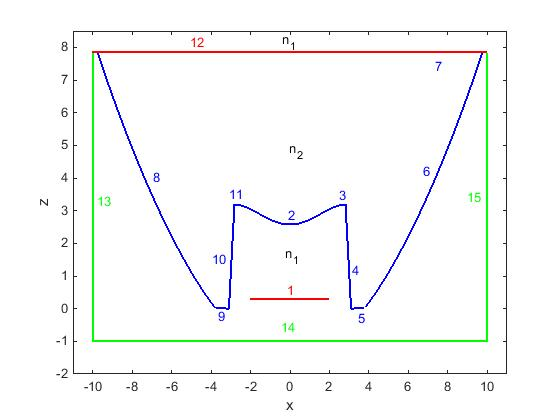
\includegraphics[width=0.7\textwidth]{tir_analytic2}
   \end{center}
    \caption{\textbf{Shape of the TIR-collimator.} Each line of the system is labeled with a number.
       $n_1 = 1$ is the refraction index of the medium (air) where the source and the target are located, and
       $n_2 = 1.5 $ the refraction index of the medium (glass) inside the optical system.} 
%The sagitta of the lens is equal to $0.6$.}
 \label{fig:analyticlens}
\end{figure}
 \begin{figure}[t]
  \begin{center}
       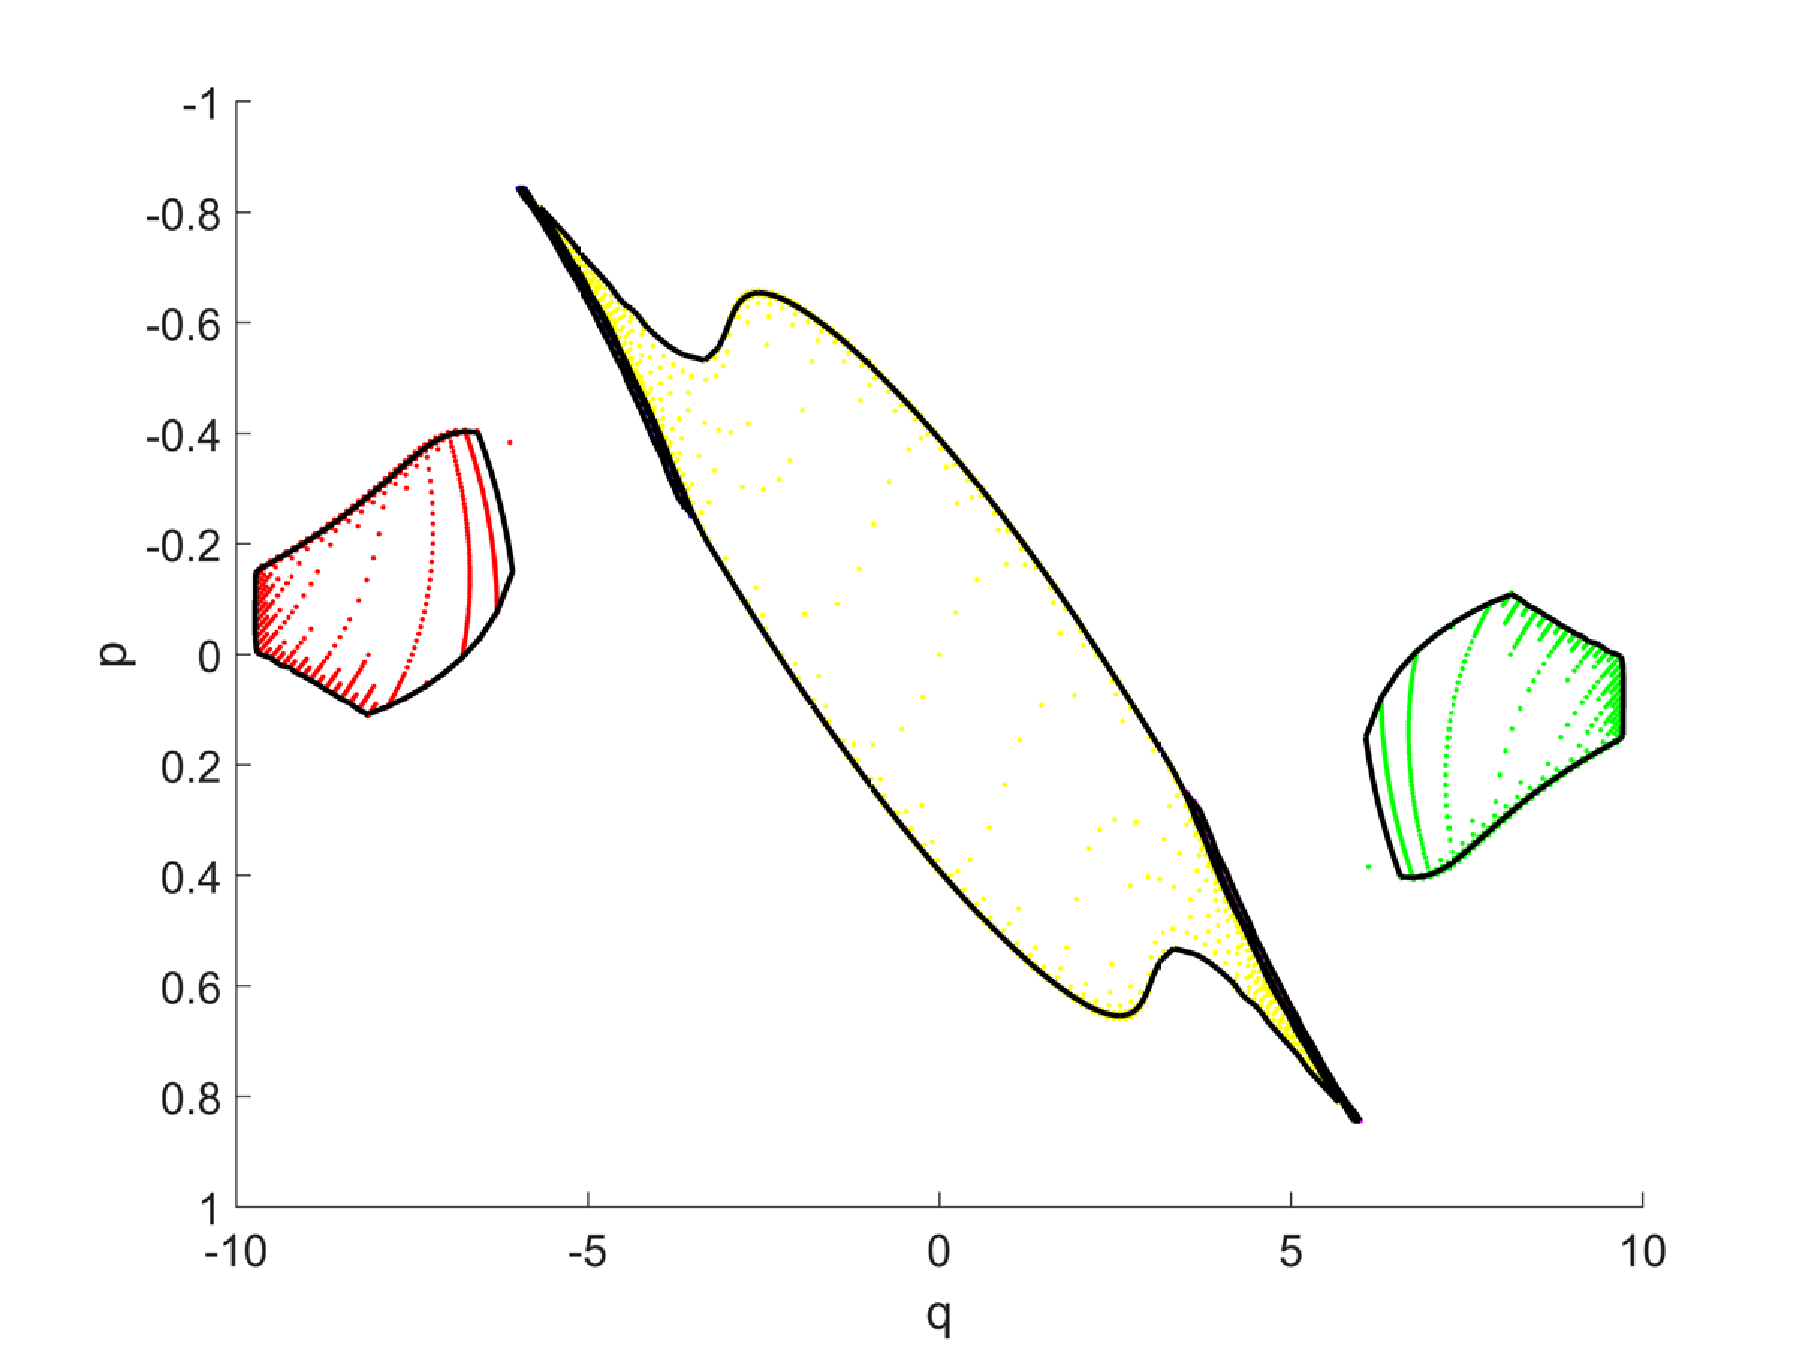
\includegraphics[width=0.7\textwidth]{boundaries_alpha3}
   \end{center}
        \caption{\textbf{Target phase space for the TIR-collimator depicted in
        Figure \ref{fig:analyticlens}.} The black line depicts the best approximation of $\partial$\set{R}{}{}$(\Pi)$ for $3\cdot 10^3$ rays. 
The $\alpha$-shapes method gives an accurate approximation of the boundaries for $\alpha_\textrm{c} = 0.9$.}
  \label{fig:Tir2}
\end{figure}
\\ \indent PS and QMC ray tracing are implemented for the TIR-collimator in Figure \ref{fig:analyticlens}. The approximated intensities $\hat{I}_{\textrm{A}}$ $(\textrm{A} = \textrm{PS}, \textrm{QMC})$ are compared to the reference intensity $\hat{I}_{\textrm{ref}}$ (QMC ray tracing with $10^7$ rays).
PS error is depicted with the red line and, QMC error is depicted with the blue line. \\ \indent
% Lets indicate with $\big(\hat{I}_{\textrm{A}, n}\big)_{n \in \mathbb{N}}$ the sequence of the approximated intensity. Every term of the sequence is calculated by increasing the number of rays, for example $\hat{I}_{\textrm{A}, 1}$ is computed tracing $\nrays = 10$ rays,   $\hat{I}_{\textrm{A}, 2}$ is computed tracing $\nrays = 100$ rays, and so on. The speed or rate of convergence of the approximate intensity $\big(\hat{I}_{\textrm{A}, n}\big)$ describes how quickly the terms of sequence $\big(\hat{I}_{\textrm{A}, n}\big)$ converge to the reference intensity $\hat{I}_{\textrm{ref}}$ by increasing the number of rays. Suppose $m$ is a real number, the sequence $\big(\hat{I}_{\textrm{A}, n}\big)$ converges to $\hat{I}_{\textrm{ref}}$ if
%\begin{equation}
%\lim_{\nrays\rightarrow \infty} \frac{|\hat{I}_{\textrm{A}, n+1}-\hat{I}_{\textrm{ref}}|}{|\hat{I}_{\textrm{A}, n}-\hat{I}_{\textrm{ref}}|^m} = \mu
%\end{equation}
%and $\mu$ is called the rate of convergence and $m$ is the order of convergence. For $m\in[0,1]$ we have the linear convergence, for $m=2$ the quadratic convergence, etc. 
%\\ \indent
Numerical results show that, for the TIR-collimator in Figure \ref{fig:analyticlens}, the number of rays needed to achieve an error of the order of $10^{-5}$ is reduced using PS ray tracing compared with QMC ray tracing. Furthermore, for a relatively small number of rays, the $\alpha$-shapes method performs better for a TIR-collimator with a flatter lens. 
\begin{figure}[t]
 \begin{center}
   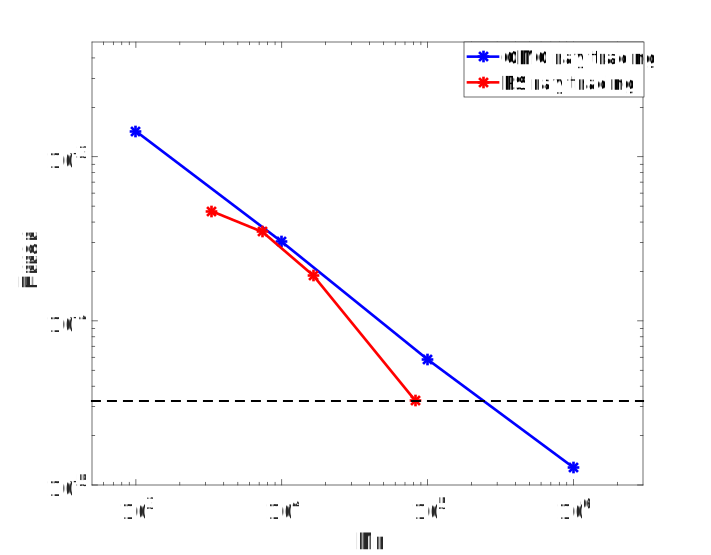
\includegraphics[width=\textwidth]{error_alpha_shapes_vs_qmc_flat}
    \end{center}
     \caption{\textbf{PS and QMC errors.}}
%The red line depicts the error using the $\alpha$-shapes method to compute the boundaries. 
%The blue line shows the error between the Monte Carlo intensity and the exact intensity.
%     The dashed black line represents a straight line with slope $-\frac{1}{2}$.
%   The dashed blue line represents a straight line with slope $-1$.}
 \label{fig:error2}
\end{figure}
\section{Conclusion}
The aim of this chapter was to detect the boundaries of the regions formed by the rays traced using $\alpha$-shapes.\\
\indent First, we reported some theory about $\alpha$-shapes which are commonly used to approximate the shape formed by a point cloud. 
These methods depend on a parameter $\alpha$ that, in most cases, can be determined only by simulations. 
\\ \indent Using \'{e}tendue conservation, we developed a new approach to detect the value of $\alpha$ that better approximates the boundaries in target PS. 
We applied $\alpha$-shapes to two different kinds of TIR-collimators. The target PS intensity was computed for both systems several times increasing every time the number of rays traced. Finally, the corresponding errors between the approximated intensities and a reference intensity was calculated. We observed that PS ray tracing allows tracing far less rays compared to QMC ray tracing. Numerical results show that using PS ray tracing the desired accuracy can be achieved reducing significantly the number of rays traced.\\ \indent 
However, we observed that the error convergence for PS ray tracing strongly depends on the design of the optical system (shapes of the region in target PS). Indeed, the accuracy of the intensity is related to the precision of the $\alpha$-shape, that is, to the choice of the parameter value of $\alpha$. For more complicated shapes in PS, more rays need to be traced for a good boundaries reconstruction.\\ \indent
In order to remove the dependence of PS ray tracing on the parameter $\alpha$, we will construct another procedure to detect the boundaries of the regions in target PS. 
The new technique is based on the triangulation refinement explained in Section \ref{sec:PS_raytracing}. The details are explained in the next chapter and numerical results are reported for several optical systems. 












































\chapter{Boundaries reconstruction based on the triangulation refinement}\label{chap:triangulation}
The purpose of this chapter is to provide an alternative approach to the $\alpha$-shapes methods for determining the boundaries $\partial \mbox{\set{R}{}{}}(\Pi)$ of the regions with positive luminance in target PS. The idea of the method is based on the triangulation refinement of the source PS explained in Chapter \ref{chap:PS}. The boundaries $\partial \mbox{\set{R}{}{}}(\Pi)$ are approximated by connecting those vertices of the triangles that follow path teh same $\Pi$. Numerical results are provided for three optical systems: the two-faceted cup, the TIR-collimator and a parabolic reflector.\\ \indent The PS method is compared to both MC and QMC ray tracing. Discussion and results are provided in the last section of this chapter.
\section{Reconstruction of the boundaries}
In Chapter \ref{chap:PS} we have seen that, using the triangulation refinement, more rays close to the boundaries are traced selecting increasingly smaller values for the parameters $\varepsilon_{\variabile{q}_1}^{\textrm{min}}$ and $\varepsilon_{\variabile{p}_1}^{\textrm{min}}$. Once the algorithm stops, only the triangles that are expected to be crossed by at least a boundary $\partial \mbox{\set{R}{}{}}(\Pi)$ are taken into account for the construction of the boundary. From now on we call these triangles the \textit{boundary triangles}. Two triangles are neighbors if they have one side in common. For each boundary triangle its neighbor is found so that an ordered sequence of triangles is constructed. Given a path $\Pi$, the corresponding boundary $\partial\mbox{\set{R}{$1$}{}}(\Pi)$ on \set{S}{}{} is approximated connecting the vertices of the boundary triangles which correspond to rays following path $\Pi$. The edge-ray principle is employed in order to define the corresponding boundaries $\partial \mbox{\set{R}{}{}}(\Pi)$ at the target.
Thus, $\partial \mbox{\set{R}{}{}}(\Pi)$ at the target are given by
\begin{equation}\map{M}{}{}(\partial\mbox{\set{R}{$1$}{}}(\Pi)):\partial\mbox{\set{R}{$1$}{}}(\Pi)\rightarrow\partial\mbox{{R}{}{}}(\Pi),\end{equation}
where $\map{M}{}{}$ is defined in (\ref{eq:map1}) and $\map{M}{}{}(\partial\mbox{\set{R}{$1$}{}}(\Pi))$ is the restriction of $\map{M}{}{}$ to $\partial\mbox{\set{R}{$1$}{}}(\Pi)$ for every path 
$\Pi$. \\\indent In this chapter we develop a criterion to establish the value of the parameters $\varepsilon_{\variabile{q}_1}^{\textrm{min}}$, $\varepsilon_{\variabile{q}_1}^{\textrm{max}}$, $\varepsilon_{\variabile{p}_1}^{\textrm{min}}$ and $\varepsilon_{\variabile{p}_1}^{\textrm{max}}$ which gives a good approximation of $\partial \mbox{\set{R}{}{}}(\Pi)$.
 Similar to the selection of $\alpha$ in the $\alpha$-shapes procedure, the triangulation parameters are chosen using \'{e}tendue conservation, i.e., conservation of area in PS. The core of our approach is the following.\\
\indent The \'{e}tendue $U_1$ at the source PS restricted to the rays that arrive at the target is calculated. If all the rays emitted by the source are received by the target, $U_1$ can be easily determined by (\ref{eq:etenduesource1}).
In case some rays do not arrive at the target and rather reach other detectors, we use (\ref{eq:etendueintegralsource}) and (\ref{eq:etenduesumsource}).
\\ \indent The \'{e}tendue $U_{\textrm{t}}$ at the target PS is calculated using (\ref{eq:etendueintegraltarget}) and (\ref{eq:etenduesumtarget}).
To do so, the triangulation refinement method is applied to the regions $\mbox{\set{R}{}{}}(\Pi)$ for a range of values of $\varepsilon_{\variabile{q}_1}^{\textrm{max}}$ and for a fixed value of $\varepsilon_{\variabile{q}_1}^{\textrm{min}}$. The parameters along the $\variabile{p}$-axis are scaled by 
\begin{equation}\label{eq:scaled_parameters}
\begin{aligned}
& \variabile{w} = \frac{\variabile{q}_1^{\textrm{max}}-\variabile{q}_1^{\textrm{min}}}{\variabile{p}_1^{\textrm{max}}-\variabile{p}_1^{\textrm{min}}},\\
&\varepsilon_{\variabile{p}_1}^{\textrm{min}}= \frac{\varepsilon_{\variabile{q}_1}^{\textrm{min}}}{\variabile{w}}, \\
&\varepsilon_{\variabile{p}_1}^{\textrm{max}}= \frac{\varepsilon_{\variabile{q}_1}^{\textrm{max}}}{\variabile{w}},
\end{aligned}
\end{equation}
 where 
$\variabile{p}_1^{\textrm{min}}$ and $\variabile{p}_1^{\textrm{max}}$ are the minimum and the maximum $\variabile{p}$-coordinate in \set{S}{}{}, and 
$\variabile{q}_1^{\textrm{min}}$ and $\variabile{q}_1^{\textrm{max}}$ are the minimum and the maximum $\variabile{q}$-coordinate in \set{S}{}{}. Every set of parameters gives a certain triangulation, for each of them an approximation of the boundaries $\partial\mbox{\set{R}{}{}}(\Pi)$ is obtained.
Next, the intersection points $(\variabile{q}^{\variabile{i}}( \Pi, \variabile{p}),\variabile{p})_{\variabile{i} = 1, \cdots, \variabile{r}}$ between $\partial\mbox{\set{R}{}{}}(\Pi)$
and the horizontal line $\variabile{p}~=~ \const{constant}$ are calculated for every path $\Pi$, and for $\variabile{p}~\in~[-1,1]$. Ordering their $\variabile{q}$-coordinates corresponding to each direction $\variabile{p}$ in ascending order, the integral in Equation (\ref{eq:etenduetarg1}) is computed.
Changing the values of the parameters, different approximations of $\partial\mbox{\set{R}{}{}}(\Pi)$ are found and, consequently, different values of $U_{\textrm{t}}$. By construction, $U_{\textrm{t}}$ is always underestimated ($U_{\textrm{t}}<U_1$) because the approximated boundaries are found joining the vertices of the \textit{boundary triangles} which are \textit{inside} the regions \set{R}{}{}$(\Pi)$.
\\ \indent To use the parameters that give a good accuracy of the target photometric variables, the difference $\Delta U = U_1-U_{\textrm{t}}$ is calculated for every value of $U_{\textrm{t}}$ found. The values of the parameters that give a small $\Delta U$ provide a triangulation refinement from which a good approximation of the target photometric variables can be computed.
\\ \indent A similar method as described here is presented by Moore \cite{moore2013methods}. In Moore's method each ray leaves a point source at the same position while the angle coordinate changes. It starts considering three sampling rays and their corresponding paths are taken into account. In case the paths are equal the rays traced are representative of all the rays inside the polygon that they describe at the target, otherwise an interpolation is required to compute the illumination pattern. This interpolation can affect the efficiency of the method. Our method employs the distribution of the rays at the target PS and avoids using any interpolation. Moreover, a criterion to stop our algorithm is provided in such a way that no more rays than necessary are traced. This makes ray tracing in PS more accurate compared to Moore's procedure. Furthermore, Moore method is not suitable for systems in which the size and the spatial distribution of the source is important as it consider only point sources.\\ \indent
The triangulation refinement method is tested for several optical systems. The results are presented next.
\section{The two-faceted cup}
In this section we apply the triangulation refinement in PS to the two-faceted cup described in Chapter \ref{chap:raytracing} and depicted in Figure \ref{fig:cup}. 
We start tracing rays inside the system using PS ray tracing as explained in Chapter \ref{chap:PS}. To avoid rays parallel to the source and rays emitted from the endpoints, we consider their initial position $\variabile{q}_1$ and initial direction $\variabile{p}_1$ such that 
\begin{equation*}
\begin{aligned}
\variabile{p}_1&\in[-1+10^{-6},1-10^{-6}] = [\variabile{p}_1^{\textrm{min}}, \variabile{p}_1^{\textrm{max}}], \\ 
\variabile{q}_1&\in[-2+10^{-12}, 2-10^{-12}] = [\variabile{q}_1^{\textrm{min}}, \variabile{q}_1^{\textrm{max}}].
\end{aligned}
\end{equation*} 
A stopping criterion for the triangulation is defined using \'{e}tendue conservation. Since the two-faceted cup is formed by only reflective lines and its target is adjacent to the left and the right reflector (it is located exactly at the top of the system),  all the rays emitted by the source arrive at the target. Thus, from (\ref{eq:etenduesource}) with $\n_1\sin(\myangle_1^{\textrm{max}})=\variabile{p}_1^\textrm{max}$ and $\variabile{a}=\variabile{q}_1^{\textrm{max}}$ follows
\begin{equation}U_1 = U \approx 8. \end{equation}
%To establish the number of rays needed to achieve a good accuracy of the target intensity, we compare the approximated $U_{\textrm{t}}$, obtained from a given number of rays, to the exact \'{e}tendue $U=U_1$. 
Ray tracing in PS is implemented by varying the parameter $\varepsilon_{\variabile{q}_1}^{\textrm{min}}$, and fixing  $\varepsilon_{\variabile{q}_1}^{\textrm{max}}$ (we choose $\varepsilon_{\variabile{q}_1}^{\textrm{max}}=1$), while the other two parameters are given by (\ref{eq:scaled_parameters}).
Every set of parameters gives a different triangulation at the source PS. The approximated boundaries are computed for several triangulations joining the vertices of the triangles crossed by a boundary. 
\begin{figure}[t]
\centering
\begin{subfigure}{.45\textwidth}
  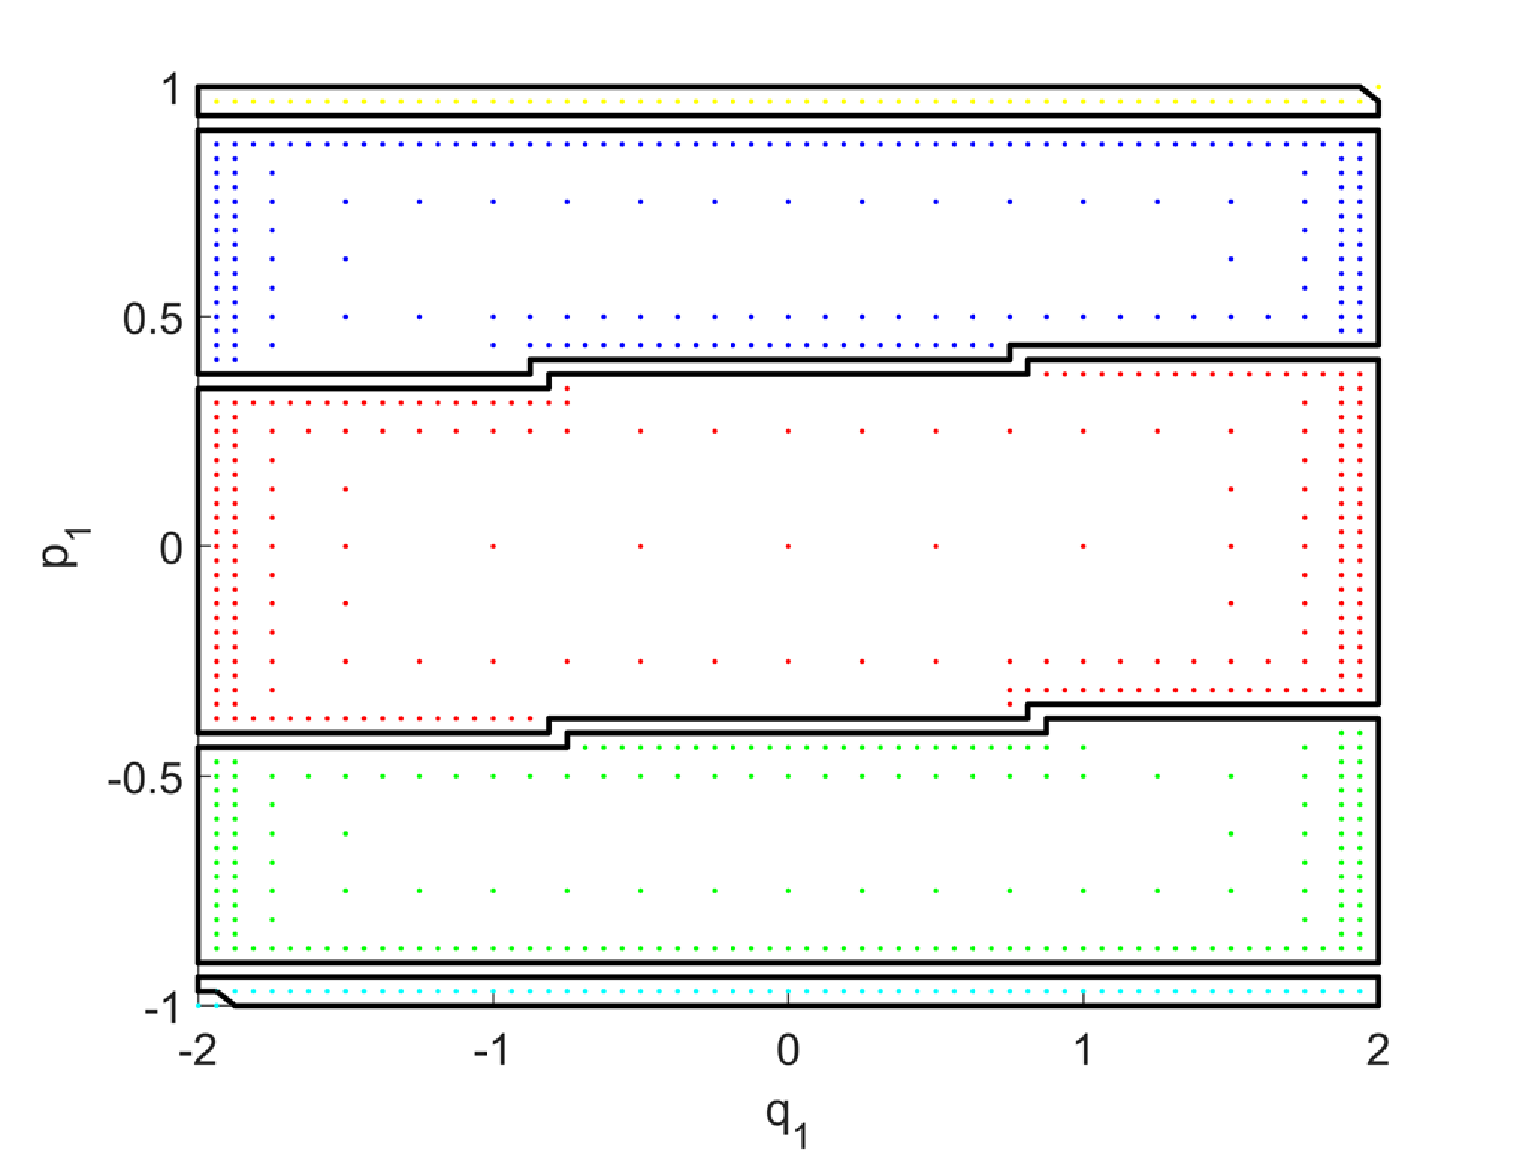
\includegraphics[width=\textwidth]{boundaries_source_triangles2}
 \caption{The black lines are the boundaries at \set{S}{}{}. $1500$ rays are traced using the triangulation refinement with $\varepsilon_{\variabile{q}_1}^{\textrm{min}}=0.1$. }
  \label{fig:boundaries_s2}
\end{subfigure}%
\hfill
\begin{subfigure}{.45\textwidth}
  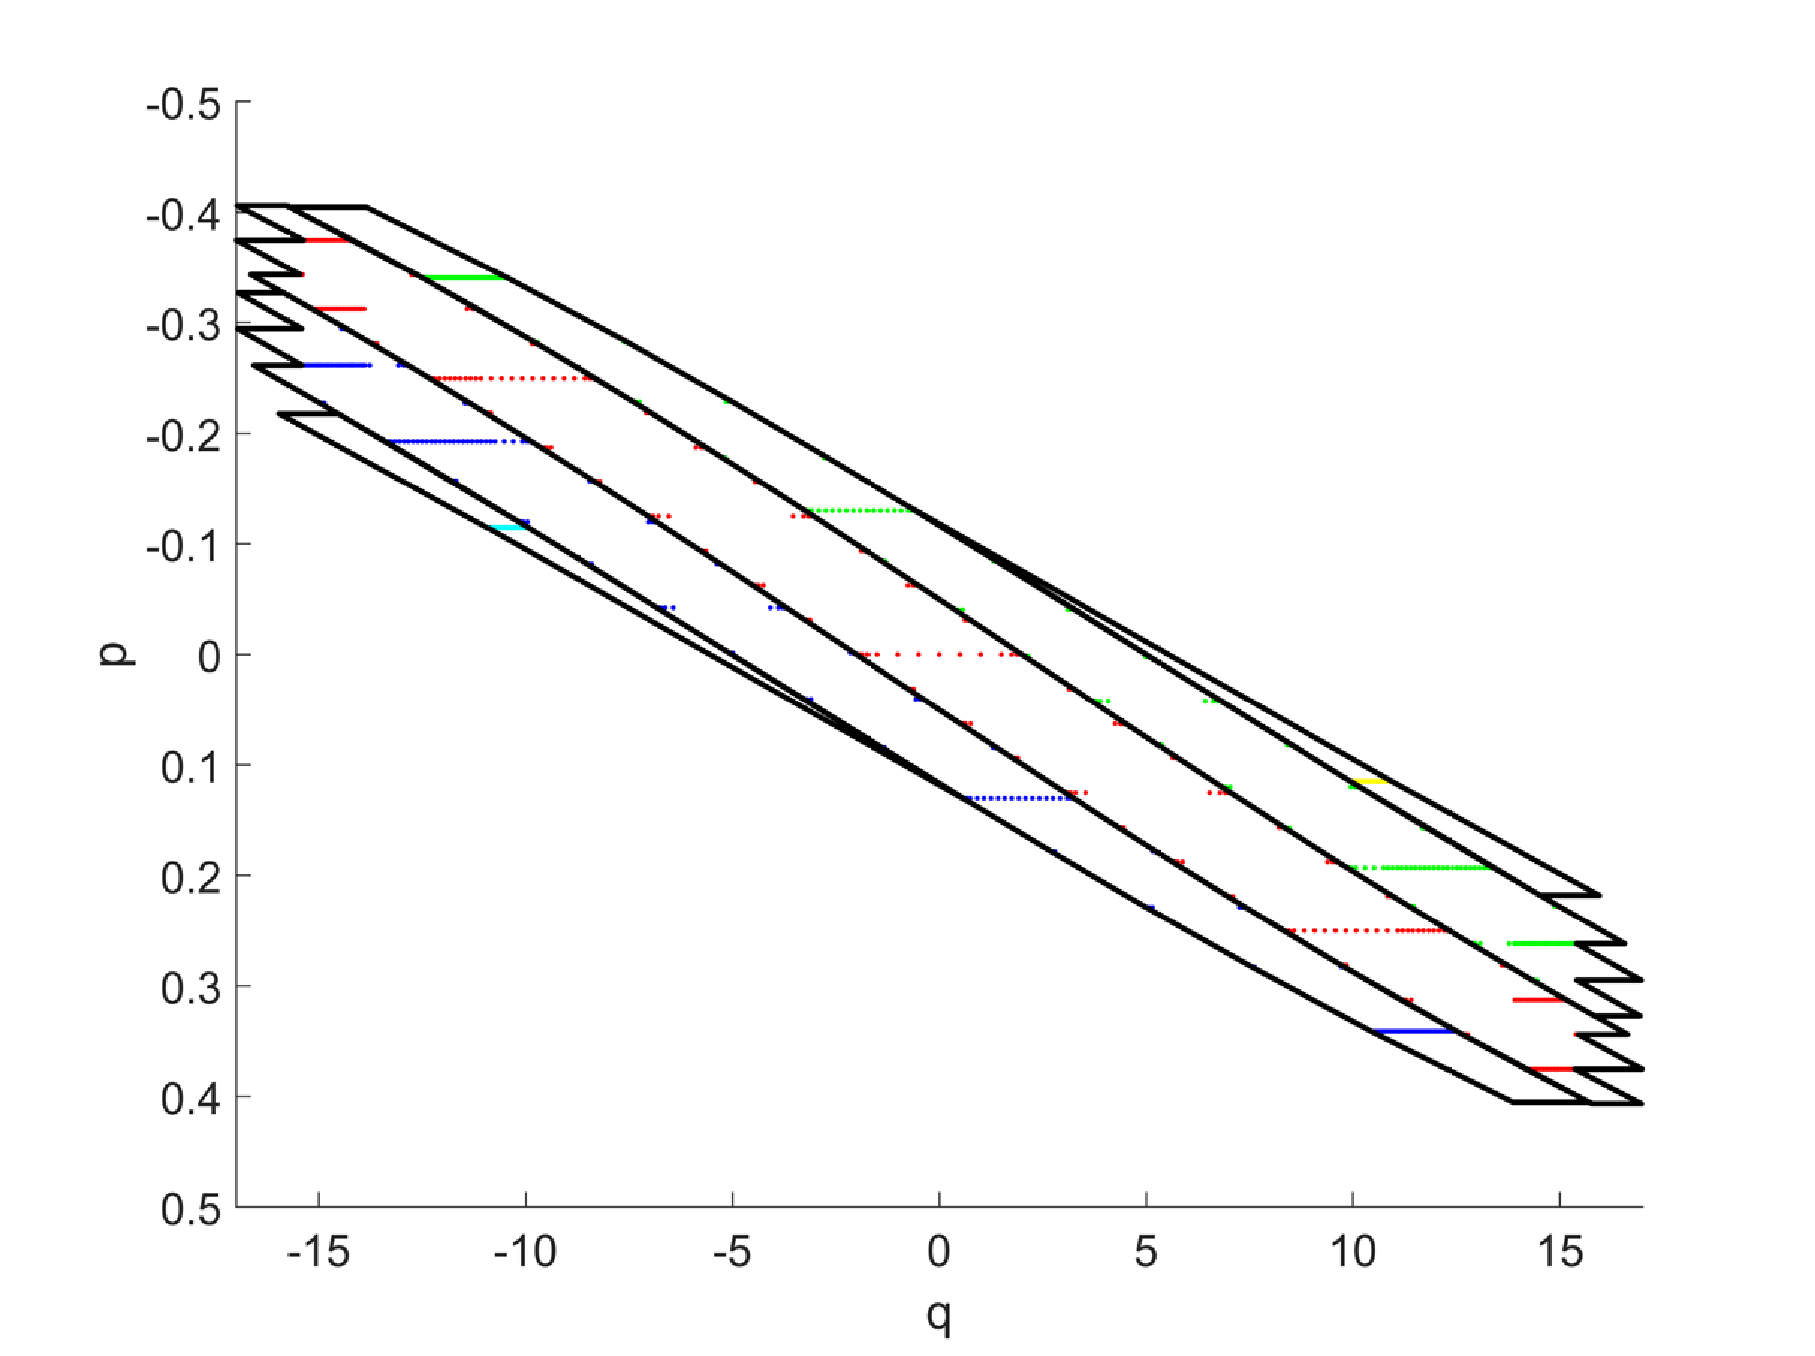
\includegraphics[width=\textwidth]{boundaries_target_triangles2}
  \caption{The black lines are the boundaries at \set{T}{}{}. $1500$ rays are traced using the triangulation refinement with $\varepsilon_{\variabile{q}_1}^{\textrm{min}}=0.1$.} %
  \label{fig:boundaries_t2}
\end{subfigure} %
\hfill
\begin{subfigure}{.45\textwidth}
  \includegraphics[width = \textwidth]{boundaries_source_triangles1}
  \caption{The black lines are the boundaries at \set{S}{}{}. $7500$ rays are traced using the triangulation refinement with $\varepsilon_{\variabile{q}_1}^{\textrm{min}}=0.025$.}
  \label{fig:boundaries_s1}
\end{subfigure}%
\hfill
\begin{subfigure}{.45\textwidth}
  \includegraphics[width=\textwidth]{boundaries_target_triangles1}
 \caption{The black lines are the boundaries at \set{T}{}{}. $7500$ rays are traced using the triangulation refinement with $\varepsilon_{\variabile{q}_1}^{\textrm{min}}=0.025$.} %
  \label{fig:boundaries_t1}
\end{subfigure}
\caption{\textbf{Boundaries at \set{S}{}{} and \set{T}{}{} of the two-faceted cup.} The approximated boundaries are computed using the triangulation refinement with two different values of $\varepsilon_{\variabile{q}_1}^{\textrm{max}}$.}
\label{fig:boundaries_cup}
\end{figure} 
\\ \indent For example, if we consider $\varepsilon_{\variabile{q}_1}^{\textrm{min}}=0.1$, $\varepsilon_{\variabile{q}_1}^{\textrm{max}}=1$ and the corresponding parameters for the $\variabile{p}$-axis given by (\ref{eq:scaled_parameters}), a triangulation with around $1500$ rays (vertices of the triangles) is found. The boundaries $\partial$\set{R}{$1$}{}$(\Pi)$ and $\partial$\set{R}{}{}$(\Pi)$ are calculated using this triangulation refinement and are depicted in black in Figures \ref{fig:boundaries_s2} and \ref{fig:boundaries_t2}, respectively. For this set of rays we found $\Delta U \approx 0.53 $. Next, we can decrease $\varepsilon_{\variabile{q}_1}^{\textrm{min}}$ to obtain a more precise approximation of $U_{\textrm{t}}$. Choosing $\varepsilon_{\variabile{q}_1}^{\textrm{min}} = 0.025$ and $\varepsilon_{\variabile{q}_1}^{\textrm{max}}=1$, a triangulation formed by around $7500$ rays is obtained. The approximated boundaries $\partial$\set{R}{$1$}{}$(\Pi)$ and $\partial$\set{R}{}{}$(\Pi)$ are depicted with black lines in Figures \ref{fig:boundaries_s1} and \ref{fig:boundaries_t1}, respectively. The approximation of the target \'{e}tendue gives $\Delta U \approx 0.13 $.
 Obviously, the boundaries computation obtained using $\varepsilon_{\variabile{q}_1}^{\textrm{min}} = 0.025$ is more accurate. 
Note that, decreasing $\varepsilon_{\variabile{q}_1}^{\textrm{min}}$, the number of rays increases. 
\\ \indent In Figure \ref{fig:etendue_cup} we show with the blue line how the target \'{e}tendue varies as a function of the parameter $\varepsilon_{\variabile{q}_1}^{\textrm{min}}$. The exact \'{e}tendue $U=8$ is depicted with the red line and it is computed using Equation (\ref{eq:etenduetarg1}). By decreasing $\varepsilon_{\variabile{q}_1}^{\textrm{min}}$ an increase of $U_{\textrm{t}}$ is observed. %Furthermore, by construction, $U_{\textrm{t}}$ is always underestimated because the approximated boundaries are found joining the vertices of the \textit{boundaries triangles} which are \textit{inside} the regions \set{R}{}{}$(\Pi)$.
 \begin{figure}[t]
  \center
  \includegraphics[width= 0.8\textwidth]{etendue_cup_epsilon}
  \caption{\textbf{Etendue for the two-faceted cup.} The total \'{e}tendue as an area in PS is depicted with the red line. The approximated \'{e}tendue for a range of values of 
$\varepsilon_{\variabile{q}_1}^{\textrm{min}}$ is shown with the blue line.}
  \label{fig:etendue_cup}
\end{figure}
In Figure \ref{fig:etendue_cup} we show the approximation of $U_{\textrm{t}}$ for at most around $1.2 \cdot 10^5$ rays traced using PS ray tracing with parameters $\varepsilon_{\variabile{q}_1}^{\textrm{min}}=0.8\cdot 10^{-4}$, $\varepsilon_{\variabile{q}_1}^{\textrm{max}}=1$, $\varepsilon_{\variabile{p}_1}^{\textrm{min}}=\varepsilon_{\variabile{q}_1}^{\textrm{min}}/2$ and $\varepsilon_{\variabile{p}_1}^{\textrm{max}}= \varepsilon_{\variabile{q}_1}^{\textrm{max}}/2$. We expect that further decreasing $\varepsilon_{\variabile{q}_1}^{\textrm{min}}$ the value of $U_{\textrm{t}}$ becomes more precise. 
\\ \indent The PS intensity $\hat{I}_{\textrm{PS}}$ with $1.2 \cdot 10^5$ rays is calculated from Equation (\ref{eta2}). The intensity profile is shown in Figure \ref{fig:intensity_cup_triangulation} with the red line. In the same graph we show the reference intensity $\hat{I}_{\textrm{ref}}$ with the dotted blue line. For the two-faceted cup the reference intensity is actually the exact intensity ($\hat{I}_{\textrm{ref}}= \hat{I}_{\textrm{exact}}$). 
 \begin{figure}[t]
  \center
  \includegraphics[width= 0.8\textwidth]{intensity_cup_triangulation}
  \caption{\textbf{Intensity profile at the target of the two-faceted cup.} The reference intensity is the exact intensity. The PS intensity is computed using the triangulation refinement with $\varepsilon_{\variabile{q}_1}^{\textrm{min}}=0.8\cdot 10^{-4}$, $\varepsilon_{\variabile{q}_1}^{\textrm{max}}=1$, $\varepsilon_{\variabile{p}_1}^{\textrm{min}}=\varepsilon_{\variabile{q}_1}^{\textrm{min}}/2$ and $\varepsilon_{\variabile{p}_1}^{\textrm{max}}= \varepsilon_{\variabile{q}_1}^{\textrm{max}}/2$. Around $1.2 \cdot 10^5$ rays are traced.}
  \label{fig:intensity_cup_triangulation}
\end{figure}
\\ \indent 
Finally, we compare PS ray tracing with both MC and QMC ray tracing by computing the error between the approximated intensities $\hat{I}_{\textrm{A}}  (\textrm{A}= \textrm{MC}, \textrm{QMC}, \textrm{PS})$ and the exact intensity $\hat{I}_{\textrm{ref}}$ using (\ref{eq:error}). For the error calculation we use (\ref{eq:error}) with $\nbin = 100$. The results are shown in Figure \ref{fig:error_cup_triangulation} where the MC, QMC and PS intensity are depicted with the green, blue and red line, respectively.
 \begin{figure}[t]
  \center
  \includegraphics[width= \textwidth]{error_cup_triangulation}
  \caption{\textbf{Error plot for the two-faceted cup.} The errors between the approximated intensities $\hat{I}_{\textrm{A}} (\textrm{A}= \textrm{MC}, \textrm{QMC}, \textrm{PS})$ and the exact intensity $\hat{I}_{\textrm{exact}}$.}
  \label{fig:error_cup_triangulation}
\end{figure}
The graph shows that using PS ray tracing in combination with the triangulation refinement admits tracing far less rays compared to MC ray tracing.
A comparison between QMC ray tracing and PS ray tracing shows that more rays are needed in PS. Indeed, although the shapes of all the regions \set{R}{}{}$(\Pi)$ are very smooth, their boundaries at the edge of the target phase space \set{T}{}{} are difficult to approximate by triangles. With the triangulation refinement, the vertical straight lines at the edge of \set{T}{}{} are always approximated by a broken line. However, the two-faceted cup is a very simple system and QMC ray tracing does not requires a large number of rays to obtain the desired accuracy. \\ \indent Nevertheless, PS ray tracing has a big advantage compared to QMC ray tracing. Indeed, as we have seen in Chapter \ref{chap:raytracing}, MC and QMC ray tracing are binning procedures. Therefore, the MC and QMC intensities are given by the average over every bin and the error also depends on the number of bins. % according to Equations \ref{} \ref{}
PS ray tracing gives a pointwise intensity along all possible directions. In the simulations shown in this thesis we always compute the average PS intensity. This is needed to give a fair comparison of PS ray tracing versus MC and QMC ray tracing. It is very important to observe that no error related to the number of bins is involved in the PS procedure. \\ \indent
To investigate in more detail the performance of PS ray tracing, we test the method for more complicated systems. In the next paragraph we present the results for a TIR-collimator. 
\section{A TIR-collimator}
In this section we provide the results of PS ray tracing for a TIR-collimator, using the triangulation refinement to compute the boundaries $\partial$\set{R}{}{}$(\Pi)$ in target PS. In particular, we consider the TIR-collimator depicted in Figure \ref{fig:analyticlens}. Since this system is located in two different media (air and glass), also the refraction law plays a role in the ray tracing procedure. We run PS ray tracing for the TIR-collimator several times gradually increasing the number of rays, i.e., gradually decreasing the values of the parameters $\varepsilon_{\variabile{q}_1}^{\textrm{min}}, \varepsilon_{\variabile{q}_1}^{\textrm{max}}, \varepsilon_{\variabile{p}_1}^{\textrm{min}}$ and $\varepsilon_{\variabile{p}_1}^{\textrm{max}}$ in the triangulation. In order to trace more rays close to the boundaries, we decide to vary only the values of $\varepsilon_{\variabile{q}_1}^{\textrm{min}}$ and $ \varepsilon_{\variabile{p}_1}^{\textrm{min}}$ while fixing the values of $ \varepsilon_{\variabile{q}_1}^{\textrm{max}}$ and $ \varepsilon_{\variabile{p}_1}^{\textrm{max}}$ as the last two are responsible of the number of rays inside the regions \set{R}{}{}$(\Pi)$. Every ray traced has initial position coordinate $\variabile{q}_1\in[-\variabile{a}, \variabile{a}]$ with $\variabile{a}=2$ and the initial direction coordinate $\variabile{p}_1\in[-1,1]$. Therefore, the source PS of the TIR-collimator is the rectangular domain \set{S}{}{}$= [-2, 2] \times [-1, 1]$. The parameters $\varepsilon_{\variabile{p}_1}^{\textrm{min}}$ and $\varepsilon_{\variabile{p}_1}^{\textrm{max}}$ are scaled as in Equation (\ref{eq:scaled_parameters}).
\\ \indent To determine the triangulation refinement that gives a good approximation of the target intensity we compare $U_1$ (source \'{e}tendue) to $U_{\textrm{t}}$ (target \'{e}tendue) and use \'{e}tendue conservation. In this case, not all light emitted by the source of the TIR-collimator arrives at the target. Indeed, using PS ray tracing, $\npath=7$ different paths $(\Pi_\lineai)_{\lineai=1, \cdots, \npath}$ are found but only five of them are paths from the source (line $1$) to the target (line $12$), see also Section \ref{sec:results-Tir-alpha}. Thus, we need to remove from the total area of \set{S}{}{} those parts occupied by the rays that arrive at some others detectors and not at the target. % white areas in figure...
Indicating with $A_T$ the area of each of these parts (see Section \ref{sec:results-Tir-alpha}), the source PS is given by:
\begin{equation}
U_1 = 8-2A_T\approx 7.77.
\end{equation}
The target \'{e}tendue $U_{\textrm{t}}$ is obtained from Equation (\ref{eq:etenduetarg}) for a range of values of $\varepsilon_{\variabile{q}_1}^{\textrm{min}}$ and for $\varepsilon_{\variabile{q}_1}^{\textrm{max}}=1$ fixed. The boundaries $\partial$\set{R}{}{}$(\Pi)$ are found for every value of $\varepsilon_{\variabile{q}_1}^{\textrm{min}}$ and, $U_{\textrm{t}}$ is calculated for each of these boundaries. 
The results shown in Figure \ref{fig:etendue_tir_triangulation} give the \'{e}tendue plot as a function of $\varepsilon_{\variabile{q}_{1}}^{\textrm{min}}$.
 \begin{figure}[t]
  \center
  \includegraphics[width = 0.8\textwidth]{etendue_tir_triangulation}
  \caption{\textbf{Etendue of the TIR-collimator.} A comparison between $U_1$ and $U_{\textrm{t}}$ shows that by decreasing the value of $\varepsilon_{\variabile{q}_{1}}^{\textrm{min}}$, $\Delta U= U_1-U_{\textrm{t}}$ decreases.}
  \label{fig:etendue_tir_triangulation}
\end{figure}
\\ \indent 
The best approximation of $U_{\textrm{t}}$ shown in the previous graph is obtained using $\varepsilon_{\variabile{q}_1}^{\textrm{min}}=1.6\cdot 10^{-3}$, tracing around $1.62 \cdot 10^5$ rays. The boundaries $\big(\partial\mbox{\set{R}{$1$}{}}(\Pi_{\lineai})\big)_{\lineai = 1, \cdots, 5}$ and $\big(\partial\mbox{\set{R}{}{}}(\Pi_{\lineai})\big)_{\lineai = 1, \cdots, 5}$ of the regions formed by these rays are shown in Figure \ref{fig:boundaries_TIR_triangulation} with red lines (see also Figure \ref{fig:Tir2} for comparison). 
\begin{figure}[h]
 \begin{subfigure}[t]{0.5\textwidth}
\centering
    \includegraphics[width=\textwidth]{boundaries_triang_source_tir}
    \caption{Boundaries at the source PS.}
    \label{fig:boundaries_triang_source_tir}
\end{subfigure}
\hfill
\begin{subfigure}[t]{0.5\textwidth}
\centering
    \includegraphics[width = \textwidth]{boundaries_triang_targ_tir}
    \caption{Boundaries at the target PS.}
    \label{fig:boundaries_triang_target_tir}
\end{subfigure}
\caption{\textbf{Boundaries at \set{S}{}{} and \set{T}{}{} of the TIR-collimator.} The red lines show the boundaries found using $\varepsilon_{\variabile{q}_1}^{\textrm{min}}=1.6\cdot 10^{-3}, \varepsilon_{\variabile{q}_1}^{\textrm{max}}=1, \varepsilon_{\variabile{p}_1}^{\textrm{min}}=\varepsilon_{\variabile{q}_1}^{\textrm{min}}/2$ and $\varepsilon_{\variabile{p}_1}^{\textrm{max}} = \varepsilon_{\variabile{q}_1}^{\textrm{max}}/2$.}
 \label{fig:boundaries_TIR_triangulation}
\end{figure}
 \\ \indent 
The target PS intensity $\hat{I}_{\textrm{PS}}$ is computed and is compared with a reference intensity $\hat{I}_{\textrm{ref}}$ which is given by QMC ray tracing with $10^7$ rays (as the exact intensity for the TIR-collimator is unknown). The profile of the two intensities is given in Figure \ref{fig:intensity_tir_triangulation}.
 \begin{figure}[ht]
  \center
  \includegraphics[width= 0.8\textwidth]{intensity_tir_triangulation}
  \caption{\textbf{Target intensity for the TIR-collimator.} The PS intensity $\hat{I}_{\textrm{PS}}$ is computed using PS ray tracing with around $1.62\cdot 10^5$ rays. The reference intensity $\hat{I}_{\textrm{ref}}$ is obtained by QMC ray tracing with $10^7$ rays.}
  \label{fig:intensity_tir_triangulation}
\end{figure}
\\ \indent
To validate our method, PS ray tracing is compared to both MC and QMC ray tracing. The error between the approximated intensities $\hat{I}_{\textrm{A}} (\textrm{A}=\textrm{QMC}, \textrm{MC}, \textrm{PS})$ and the reference intensity $\hat{I}_{\textrm{ref}}$ as a function of the number of rays traced is calculated. The error plot is shown in a logarithmic scale in Figure \ref{fig:error_tir_triangulation} where the MC, QMC and PS convergences are shown with the green, the blue and the red line, respectively. The black dotted line is a line with slope $-\frac{1}{2}$, the blue dotted line has slope $-1$.The graph shows that MC ray tracing converges, for $\nrays \rightarrow \infty$, with an order of $\mathcal{O}\big(\frac{1}{\sqrt{\nrays}}\big)$, while both PS and QMC ray tracing have a speed of convergence of the order $\mathcal{O}\big(\frac{1}{\nrays}\big)$. 
Note that PS ray tracing allows tracing $10^2$ times less rays compared to MC ray tracing and almost $10$ times less rays compared to QMC ray tracing to obtain an error of $10^{-4}$.
 \begin{figure}[h!]
  \center
  \includegraphics[width= \textwidth]{error_nr_triangulation_tir}
  \caption{\textbf{Error as a function of the number of rays for the TIR-collimator.} The reference intensity $\hat{I}_{\textrm{ref}}$ is obtained by QMC ray tracing with $10^7$ rays.}
  \label{fig:error_tir_triangulation}
\end{figure}
\begin{figure}[h!]
  \center
  \includegraphics[width= \textwidth]{error_tir_triangulation_time}
  \caption{\textbf{Error as a function of the CPU-time for the TIR-collimator.} The reference intensity $\hat{I}_{\textrm{ref}}$ is obtained by QMC ray tracing with $10^7$ rays.}
  \label{fig:error_tir_triangulation_time}
\end{figure}
\\ \indent Finally, in order to show the advantages of PS ray tracing in terms of the computational time, we provide an error convergence as a function of the CPU-time for all the three methods (MC, QMC and PS raytracing) shown in Figure \ref{fig:error_tir_triangulation_time}. The choice of the colors is consistent with Figure \ref{fig:error_tir_triangulation}. We observe that PS ray tracing outperforms both MC and QMC ray tracing. PS ray tracing is approximately $10^2$ times faster than MC ray tracing and $10$ times faster than QMC ray tracing. \\ \indent The results shown in Figures \ref{fig:error_tir_triangulation} and \ref{fig:error_tir_triangulation_time} are reported in Tables \ref{tab:ps_error_triangulation} and \ref{tab:mc_error_triangulation}.
\begin{table}[t] 
\centering
\caption{\bf Errors of the PS intensity for the TIR-collimator}
\begin{tabular}{lllll}
 \hline   $\varepsilon_{\variabile{q}}^{\textrm{max}} $  & $\nrays$ & Etendue & PS error & PS CPU-time (sec.) \\
  \hline 
 $0.05$ & $3\,547$   & $7.50$   &  $1.75\cdot10^{-4}$ & $1.98$\\
$0.025$  & $8\,055$    & $7.61$    & $1.49\cdot 10^{-4}$ & $4.69$ \\
$0.125$  & $17\,300$    & $7.69$  & $8.68\cdot 10^{-5}$ & $10.61$\\
 $6.3 \cdot 10^{-3}$  & $38\,300$  & $7.73$   & $4.43\cdot 10^{-5}$ & $26.56$\\
 $3.1 \cdot 10^{-3}$ & $79\,600$  & $7.75$    & $2.27\cdot 10^{-5}$ & $83,21$\\
$1.6 \cdot 10^{-3}$ & $162\,300$  & $7.76$    & $1.20\cdot 10^{-5}$ & $240.53$\\
 \hline
 \end{tabular}
\label{tab:ps_error_triangulation}
 \end{table}
\begin{table}[t] \label{tab:table_tir_triangulation}
\centering
\caption{\bf Errors of the MC and QMC intensities for the TIR-collimator}
\begin{tabular}{lllll}
 \hline   $\nrays$ & MC error & MC CPU-time (sec.) & QMC error  & QMC CPU-time (sec.)\\
  \hline 
 $10^3$     & $2.09\cdot 10^{-3}$ & $2.73$ & $1.43\cdot10^{-3}$    & $2.63$\\
 $10^4$     & $6.42\cdot 10^{-4}$ & $25.98$ & $3.03\cdot 10^{-4}$   & $25.84$\\
 $10^5$     & $1.92\cdot 10^{-4}$ & $259.92$ & $5.82\cdot 10^{-5}$   & $258.28$\\
 $10^6$     & $7.45\cdot 10^{-5}$ & $2585.83$   & $1.28\cdot 10^{-5}$   & $2482.67$\\
 \hline
 \end{tabular}
 \label{tab:mc_error_triangulation}
 \end{table}
%\begin{table}[t] 
%\centering
%\caption{\bf Errors of the QMC intensity for the TIR-collimator}
%\begin{tabular}{lllll}
% \hline  $\nrays$\;  & QMC error  & CPU-time (sec.)\\
%  \hline 
% $10^3$   & $1.43\cdot10^{-3}$    & $2.63$  \\
%$10^4$    & $3.03\cdot 10^{-4}$   & $25.84$   \\
%$10^5$    & $5.82\cdot 10^{-5}$   & $258.28$  \\
% $10^6$   & $1.28\cdot 10^{-5}$   & $2482.67$  \\
% \hline
% \end{tabular}
% \label{tab:qmc_error_triangulation}
% \end{table}
%Using PS ray tracing an error equal to $10^{-4}$ is achieved tracing almost $10$ time less compared to QMC ray tracing and $100$ times less rays compared to QMC ray tracing. 
Next, we show the result for a system in which more than $5$ paths are possible. 
In particular we present the results for an optical system for which multiple reflections between rays and the mirrors occur.
\section{A Parabolic reflector}
In this section we show an example of a parabolic reflector which is depicted in Figure \ref{fig:PR}.
 It consists of a source \point{S} (line $1$), a target \point{T} (line $4$) parallel to \point{S} and two reflectors (lines $2$ and $3$) which are arcs of the same parabola. 
  The minimum of the parabola is located at the point with $\variabile{x}$-coordinate equal to $0$. $\point{S}=[\variabile{-a}, \variabile{a}]$ (with $\variabile{a}=2$) and $\point{T}=[-\variabile{b},\variabile{b}]$ (with $\variabile{b}=17$) are lines perpendicular to the optical axis (\variabile{z}-axis) and are located at $\variabile{z}=0$ and $\variabile{z}=40$, respectively.
All the optical lines are located in air, therefore the index of refraction ${n}=1$ for every line.
The optical axis of the system in Figure \ref{fig:PR} corresponds to the \variabile{z}-axis.
\begin{figure}[h!]
\centering
\includegraphics[width=0.7\textwidth]{parabolic_reflector}
\caption{\textbf{A parabolic reflector.}  Each line of the system is labeled with a number.
   The source \point{S}$= [2,2]$ (line $1$) is located on the $\variabile{x}$-axis.
   The target \point{T}$= [-17, 17]$ (line $4$) is parallel to the source and is located at a height $ \variabile{z}= 40$.
   The left and right reflectors (lines $2$ and $3$) are arcs of the same parabola.}
\label{fig:PR}
\end{figure}
We trace rays in PS with source direction coordinates $\variabile{p}_1 \in [-1,1]$ and source position coordinates $\variabile{q}_1\in[-\variabile{a}+\varepsilon,\variabile{a}-\varepsilon]$ where $\varepsilon>0$ is a small number. In particular we take $\varepsilon = 10^{-12}$.\\ \indent As an example we show the triangulation refinement obtained for the parameters $$\varepsilon_{\variabile{q}_1}^{\textrm{min}} = 0.025, \; \varepsilon_{\variabile{q}_1}^{\textrm{max}} = 0.5, \; \varepsilon_{\variabile{p}_1}^{\textrm{min}} = \varepsilon_{\variabile{q}_1}^{\textrm{min}}/2, \mbox{ and }  \varepsilon_{\variabile{p}_1}^{\textrm{max}} = \varepsilon_{\variabile{q}_1}^{\textrm{max}}/2, $$ for which around $8300$ rays are traced in PS. Their distribution at \set{S}{}{} and \set{T}{}{} is shown in Figures \ref{fig:source_triang_pr} and \ref{fig:target_triang_pr}, respectively. 
\begin{figure}[h]
 \begin{subfigure}[h]{0.47\textwidth}
\centering
    \includegraphics[width=\textwidth]{pr_source}
    \caption{Source PS \set{S}{}{} $= [-\variabile{a}+\varepsilon,\variabile{a}-\varepsilon]\times[-1,1]$}
    \label{fig:source_triang_pr}
\end{subfigure}
\hfill
\begin{subfigure}[h]{0.47\textwidth}
\centering
    \includegraphics[width = \textwidth]{pr_target}
    \caption{Target PS \set{T}{}{} $= [-\variabile{b},\variabile{b}]\times[-1,1]$}
    \label{fig:target_triang_pr}
\end{subfigure}
\caption{\textbf{Rays distribution at \set{S}{}{} and \set{T}{}{} of the parabolic reflector.} Around $8300$ rays are traced using PS ray tracing with parameters $\varepsilon_{\variabile{q}_1}^{\textrm{min}} = 0.025, \; \varepsilon_{\variabile{q}_1}^{\textrm{max}} = 0.5, \; \varepsilon_{\variabile{p}_1}^{\textrm{max}} = \varepsilon_{\variabile{q}_1}^{\textrm{min}}/2, \mbox{ and }  \varepsilon_{\variabile{p}_1}^{\textrm{min}} = \varepsilon_{\variabile{q}_1}^{\textrm{max}}/2$ . $17$ different paths are found, each of them correspond to a certain number of reflections.}
 \label{fig:phase_space_pr}
\end{figure} The distribution of the rays in PS gives information about the paths they follow. We note that for the parabolic reflector many paths are found. Every path corresponds to a given number of reflections. Rays can have multiple reflections at lines $2$ and $3$ before arriving at the target. The parameters used in the triangulation refinement establish not only the number of rays traced but also the number of paths detected. For instance, for the values of the parameters defined above, the triangulation refinement is able to detect $17$ different paths. This means that up to $8$ multiple reflections occur between the rays and the two mirrors. Counting the number of rays that follow a given path $\Pi$, we can calculate the fraction of rays for every path. For example, tracing around $8300$ rays, the percentage of the rays that have $8$ multiple reflections along one of the two reflectors is around $0.13\%$. Rays that reflect many times before reaching the target do not give a significant contribution to the target intensity. Decreasing the value of the parameter $\varepsilon_{\variabile{q}_1}^{\textrm{min}}$, more paths can be found. The more reflections occur the smaller the correspond area in PS is. In order to find as many path as possible, also the parameter $\varepsilon_{\variabile{q}_1}^{\textrm{max}}$ needs to be decreased. Increasing the number of reflections considered, the corresponding regions in PS become smaller and smaller, see Figure \ref{fig:phase_space_pr}. \\ \indent Like for the optical systems considered in the previous sections, a stopping criterion of the triangulation refinement is determined for the parabolic reflector. Etendue conservation is used in order to find the values of the parameters that give a good approximation of the boundaries of the regions with positive luminance in PS. For the parabolic reflector in Figure \ref{fig:PR} all the rays that leave the source arrive at the target. Indeed, line $2$ and $3$ can only reflect rays (refraction law is not involved) and the target \'{e}tendue is equal to the source \'{e}tendue. From Equation (\ref{eq:etenduesource}) we obtain:
\begin{equation}
U = U_1 = 4(\variabile{a}-\varepsilon)\approx 8.
\end{equation}
A range of values of $\varepsilon_{\variabile{q}_1}^{\textrm{min}}$ and $\varepsilon_{\variabile{q}_1}^{\textrm{max}}$ is considered (the triangulation parameters for the $\variabile{p}$-axis depend on the $\variabile{q}$-axis parameters according to Equation (\ref{eq:scaled_parameters})). For each couple of values, an approximation of the boundaries $\partial$\set{R}{}{}$(\Pi)$ is found for every path $\Pi$ as explained. $U_{\textrm{t}}$ is calculated for the approximated boundaries using Equation (\ref{eq:etenduetarg}). In Table \ref{tab:etendue_pr} we show how the number of rays traced, the paths found and the value for the target \'{e}tendue depend on the triangulation parameters.
We observe that, decreasing $\varepsilon_{\variabile{q}_1}^{\textrm{min}}$ and $\varepsilon_{\variabile{q}_1}^{\textrm{max}}$ the number of both the rays traced and the paths found increases. A maximum of $17$ different paths are detected. Furthermore, the value of $U_{\textrm{t}}$ gets closer and closer to the exact \'{e}tendue $U$.
\begin{table}[t] 
\centering
\caption{\bf Results of the triangulation refinement.}
\begin{tabular}{lllll}
 \hline   $\varepsilon_{\variabile{q}}^{\textrm{min}} $  & $\varepsilon_{\variabile{q}}^{\textrm{max}}$ & $\nrays$ & $\npath$ & Etendue \\
  \hline 
 $0.2$ & $1$   & $643$   &  $11$ & $5.71$\\
$0.1$ & $1$   & $1\,573$   &  $15$ & $7.23$\\
$0.025$  & $0.5$    & $8\,357$  & $17$ & $7.65$\\
 $0.025/2$  & $0.5/2$  & $18\,613$   & $17$ & $7.82$\\
$0.025/4$  & $0.5/4$  & $40\,465$   & $17$ & $7.82$\\
 $0.025/8$ & $0.5/8$  & $86\,529$    & $17$ & $7.96$\\
$0.025/16$ & $0.5/16$  & $185\,581$    & $17$ & $7.98$\\
 \hline
 \end{tabular}
 \label{tab:etendue_pr}
 \end{table}
\\ \indent Using the triangulation refinement that gives the best \'{e}tendue approximation, we calculate the target PS intensity $\hat{I}_{\textrm{PS}}$ from Equation (\ref{eq:PSintensity}).
The intensity profile is shown with the red line in Figure \ref{fig:intensity_pr}. The PS intensity is compared to a reference intensity $\hat{I}_{\textrm{ref}}$, computed using QMC ray tracing with $10^7$ rays. $\hat{I}_{\textrm{ref}}$ is depicted Figure \ref{fig:intensity_pr} with the dotted blue line. The graph shows that the two intensities coincide.
 \begin{figure}[t]
  \center
  \includegraphics[width = \textwidth]{intensity_pr}
  \caption{\textbf{Target intensity of the parabolic reflector.} For the PS intensity the parameters $\varepsilon_{\variabile{q}_1}^{\textrm{min}}=1.56\cdot 10^{-3}$, $\varepsilon_{\variabile{q}_1}^{\textrm{max}}=3.13\cdot 10^{-2}$, $\varepsilon_{\variabile{p}_1}^{\textrm{min}}=\varepsilon_{\variabile{q}_1}^{\textrm{min}}/2$, and $\varepsilon_{\variabile{p}_1}^{\textrm{max}}=\varepsilon_{\variabile{q}_1}^{\textrm{max}}/2$ are used. Around $8.15 \cdot 10^{4}$ rays are traced in PS. For the reference intensity QMC ray tracing with $10^7$ rays is implemented.}
  \label{fig:intensity_pr}
\end{figure}
\begin{table}[t] \label{tab:table_pr_triangulation}
\centering
\caption{\bf Errors of the PS intensity for the parabolic reflector}
\begin{tabular}{lll}
 \hline   $\nrays$ & PS error & CPU-time (sec.) \\
  \hline 
 $643$        & $5.18\cdot10^{-4}$ & $0.24$\\
 $1\,573$       & $8.99\cdot 10^{-4}$ & $0.48$\\
 $8\,357$     & $2.87\cdot 10^{-4}$ & $2.40$ \\
 $18\,613$     & $1.38\cdot 10^{-4}$ & $5.48$\\
 $40\,465$   & $5.80\cdot 10^{-5}$ & $16.14$\\
 $86\,529$    & $2.90\cdot 10^{-5}$ & $55.04$\\
 $185\,581$   & $1.66\cdot 10^{-5}$ & $245.97$\\
 \hline
 \end{tabular}
\label{tab:table_pr_triangulation}
 \end{table}
\\ \indent 
Now, our method is compared to both MC and QMC ray tracing. 
The error between the approximate intensities $\hat{I}_{\textrm{A}}(\textrm{A}=\textrm{PS}, \textrm{MC}, \textrm{QMC})$ and the reference intensity is calculated. In Figure \ref{fig:error_rays_pr} the error as a function of the number of rays traced is shown for the three methods.
The green line represents the MC error, the blue line pictures the QMC error and the red line depicts the PS error. The errors are shown in a logarithmic scale, the dotted black line has slope $-1/2$, the dotted blue line has slope $-1$. Like for the other systems, MC ray tracing converges proportionally to $1/\sqrt{\nrays}$. QMC convergence is proportional to $1/\nrays$ for $\nrays \rightarrow \infty$. Less rays compared to MC ray tracing are needed in PS. In particular, to achieve an error of $10^{-4}$, around $10$ times less rays in PS are needed compared to MC and few rays less than QMC.
\begin{figure}[t]
  \center
  \includegraphics[width = \textwidth]{error_pr_100bin_rays}
  \caption{\textbf{Error as a function of the number of rays traced.} Less rays are needed using PS ray tracing compared to both MC and QMC ray tracing.}
  \label{fig:error_rays_pr}
\end{figure} 
\\ \indent
Finally, the error as a function of the CPU-time is shown in Figure \ref{fig:error_time_pr}. The MC, QMC and PS errors are depicted with the green, blue and red line, respectively. To obtain an error of the order of $10^{-5}$, PS ray tracing is $10$ times faster than MC ray tracing while becomes twice slower than QMC ray tracing. The detailed results of the numerical simulations are reported in Tables \ref{tab:mc_error_pr_triangulation} and \ref{tab:QMC_error_pr_triangulation}.
\begin{figure}[t]
  \center
  \includegraphics[width = \textwidth]{error_pr_100bin_time}
  \caption{\textbf{Error as a function of the CPU-time.} PS ray tracing has significant advantages in terms of the CPU-time compared to MC ray tracing. For the parabolic reflector the computational time is comparable with QMC ray tracing.}
  \label{fig:error_time_pr}
\end{figure} 
\begin{table}[t] 
\centering
\caption{\bf Errors of the MC intensity for the parabolic reflector}
\begin{tabular}{lll}
 \hline   $\nrays$ & MC error & CPU-time (sec.) \\
  \hline 
 $10^3$     & $1.18\cdot10^{-3}$ & $0.39$\\
 $10^4$     & $5.74\cdot 10^{-4}$ & $3.43$ \\
 $10^5$     & $1.73\cdot 10^{-4}$ & $33.13$\\
 $10^6$     & $5.79\cdot 10^{-5}$ & $328.96$\\
 $10^7$     & $1.68\cdot 10^{-5}$ & $3325.39$\\
 \hline
 \end{tabular}
 \label{tab:mc_error_pr_triangulation}
 \end{table}
\begin{table}[t] 
\centering
\caption{\bf Errors of the QMC intensity for the parabolic reflector}
\begin{tabular}{lll}
 \hline   $\nrays$ & QMC error & CPU-time (sec.) \\
  \hline 
 $10^3$     & $1.36\cdot10^{-3}$ & $0.53$\\
 $10^4$     & $2.05\cdot 10^{-4}$ & $3.44$ \\
 $10^5$     & $2.89\cdot 10^{-5}$ & $31.22$\\
 $10^6$     & $6.96\cdot 10^{-6}$ & $314.59$\\
 \hline
 \end{tabular}
 \label{tab:QMC_error_pr_triangulation}
 \end{table}
\\ \indent As explained above, MC and QMC errors also depend on the number of bins $\nbin$. In the simulations shown in this chapter we have always considered $\nbin = 100$. On the contrary, PS ray tracing calculates the intensity pointwise, nevertheless we considered $\nbin = 100$ bins at the target and we calculate the averaged normalized PS intensity over every bin in order to have a precise comparison with the binning procedures. Because of this, we expect that increasing the number of bins, the average PS intensity becomes more accurate. To verify this conjecture, we implemented MC, QMC and PS ray tracing considering a partitioning of the interval $[-1,1]$ into $\nbin = 150$ bins. The number of rays considered for the reference intensity have to be increased $(1.5)^5$ times. The averaged normalized intensities $\hat{I}_{\textrm{A}} (\textrm{A}=\textrm{MC}, \textrm{QMC}, \textrm{PS})$ found considering $\nbin=150$ bins are compared with the reference intensity $\hat{I}_{\textrm{ref}}$ (averaged and normalized) which is computed using QMC ray tracing with $7.6\, 10^7$ rays. The error as a function of the number of rays is shown in Figure \ref{fig:error_pr_150_bin}. The results show that, using PS ray tracing an error of the order of $10^{-5}$ is obtained tracing around $10^2$ times less rays than MC ray tracing and twice less rays than QMC ray tracing. We conclude that, increasing the number of bins, PS error outperforms both MC and QMC ray tracing (see also Figure \ref{fig:error_rays_pr}).
\begin{figure}[h]
  \center
  \includegraphics[width= \textwidth]{error_pr_150bins_ray}
  \caption{\textbf{Error plot for the parabolic reflector considering $\nbin=150$ bins.} Increasing the number of bins, the PS error decreases resulting in a better convergence compared to MC and QMC ray tracing.}
  \label{fig:error_pr_150_bin}
\end{figure}
\section{Discussion and conclusions}
In this chapter we presented a method to calculate the boundaries of the regions with positive luminance in PS. This method does not depend on the parameter $\alpha$ needed for the $\alpha$-shapes method presented in Chapter \ref{chap:boundaries_alpha}. Indeed, given a triangulation at the source PS, the boundaries are computed connecting the vertices of the boundary triangles, i.e., triangles crossed by a boundary, that follow the same path. Employing \'{e}tendue conservation, a stopping criterion for the triangulation refinement was developed. We applied the method to three different optical systems: the two-faceted cup, a TIR-collimator, and a parabolic reflector. Numerical results show that PS ray tracing is faster and more accurate than MC ray tracing. Compared to QMC ray tracing we observed accuracy and speed advantages of an order of magnitude with our method for the TIR-collimator. 
For the two-faceted cup, PS ray tracing has a slower convergence compared to QMC ray tracing. For the parabolic reflector PS and QMC ray tracing display similar convergence. As an example, for this system we showed that increasing the number of bins the errors decrease. 
To conclude we state that QMC ray tracing performs better than PS ray tracing for very simple optical systems, but the PS approach is more suitable for complicated optical systems.
\\ \indent In order to further improve PS ray tracing we develop a new method which employs the PS of \textit{all} the optical lines. This method is explained in the next chapter.
%We claim that PS ray tracing is also more accurate than the ray tracing procedure proposed by Moore (2013), \cite{moore2013methods}.
%The novelty of our approach compared to the method used by Moore, is briefly explained below. First, to compute the output intensity, we employ the phase space of the target. This avoids the use of any interpolation to compute the photometric variables and therefore, more accurate results are obtained.
%Second, in  all rays that leave the source start at the same position and only a sampling angular range is given. In our approach a rectangular source is considered thus, both the angular and spatial coordinates of each ray change. This extra variable can produce very irregular shapes of the regions at target phase space. To overcome this issue, we employ the edge-ray principle and we consider the regions at source phase space where the distribution of the rays is much more regular and the corresponding boundaries are easily computed.
%As a consequence, our procedure is suitable to compute the output intensity as function of both the angular or the spatial coordinates.
%Third, using the conservation of \'{e}tendue, we provided a criterion to stop the triangulation refinement. In this way we can estimate the number of rays required to obtain the desired accuracy and thus, we avoid tracing more rays than necessary.









 

%\section{The Compound Parabolic Concentrator (CPC)}
\chapter{Concatenated backward ray mapping}\label{chap:raymapping1}
In the previous chapter we have seen that PS ray tracing based on the source and the target PS constitutes an improvement of MC and QMC ray tracing. 
Now, a method that employs not only the source and the target PS but also the PS of \textit{all} the other lines that constitute the optical system is introduced. 
% Furthermore, instead of starting from the source, the new approach is an inverse method which starts considering rays on target PS.
In this chapter, we consider systems formed only by straight and reflective line segments.
All lines can be modeled as detectors of the incident light and emitters of the reflected light, they constitute
the target for incident rays and the source for reflected rays.
Moreover, we assume that the source can only emit light and the target can only receive light.
%Therefore, 
%one PS is taken into account for the source and one for the target while both the source and target phase spaces are considered for the other lines. E%
%Every line of the system (except for the source \point{S} and the target \point{T}) . 
Therefore, two different phase spaces are considered for the reflectors and one PS for
\point{S} and \point{T}. All these phase spaces are connected through a map which relates the ray coordinates on every PS. This map can be written as the concatenation of many maps which can be classified as two different kind of maps, i.e., the map that connects the source and the target PS of two \textit{different} lines and the map that connects the target and the source PS of the \textit{same} line.
Employing the inverses of these maps we are able to detect the parts of target PS illuminated by the source.
All the PS considered are divided into several regions, the boundaries of which can be determined exactly for systems formed by straight lines.
We make the assumption of a Lambertian source.
%; hence, the luminance is a positive constant inside a when different from $0$. 
As a consequence, the output intensity along a given direction is obtained from the total width of all the patches with positive luminance, measured along that direction.\\ \indent 
%In this chapter we explain the method for systems formed by straight and reflective lines segment. 
In this chapter, two different optical systems are investigated: the two-faceted cup and the so-called multi-faceted cup. Next, the details of the procedure are explained for the two-faceted-cup.
\section{Phase spaces of the two-faceted cup}\label{sec:cup_raymapping}
A two-faceted cup is introduced in Chapter \ref{chap:raytracing} and depicted in Figure \ref{fig:cup}. It is formed by a source \point{S}, a target \point{T} and two reflectors which are straight lines segments. 
Using the same notation of Chapter \ref{chap:PS}, we denote with $\mbox{\set{S}{}{}}=\mbox{\set{Q}{}{}}\times\mbox{\set{P}{}{}}$ the PS and with 
$(\variabile{q}, \variabile{p})$ the rays coordinates in \set{S}{}{}.\\ \indent
Let's now introduce some new notation. 
The source and the target PS of a line $\lineai$ are indicated with \set{S}{\lineai}{} and \set{T}{\lineai}{}, respectively. The initial rays coordinates in \set{S}{}{} are denoted with $(\pos{s,}{$1$}, \dir{s,}{$1$})$.
The coordinates of every ray that reaches the line $\lineai\in\{2, 3, 4\}$ are indicated  with $(\pos{t,}{\lineai}, \dir{t,}{\lineai})$ on \set{T}{\lineai}{}. 
In the following, to simplify the notation, we indicate the target coordinates of the rays on \set{T}{$4$}{} with (\variabile{q}, \variabile{p}) instead of $(\pos{t,}{$4$}, \dir{t,}{$4$})$.
After reflection, the ray leaves line $\lineai \in\{2, 3\}$ at the same position but with a different direction, the new ray coordinates are indicated with 
$(\pos{s,}{\lineai}, \dir{s,}{\lineai})$ on \set{S}{\lineai}{}. 
Note that $\pos{s,}{\lineai}= \pos{t,}{\lineai}$, while $\dir{s,}{\lineai}$ is obtained applying the reflection law to the direction coordinate $\dir{t,}{\lineai}$ of the incident ray.
The phase spaces \set{S}{\lineai}{} and  \set{T}{\lineai}{} of each line $\lineai$ are partitioned into different regions, (\set{S}{\lineai,}{\lineaj})$_{\lineaj=2, 3, 4}$ and (\set{T}{\lineai,}{\lineak})$_{\lineak=1, 2, 3}$, respectively, where $\lineaj\neq \lineai$ is the index of the line that is illuminated by $\lineai$ and $\lineak\neq\lineai$ is the index of the line that illuminates $\lineai$. Hence, \set{S}{\lineai,}{\lineaj}$\subset$ \set{S}{\lineai}{} is the part of \set{S}{\lineai}{} corresponding to rays that illuminate line $\lineaj$, and \set{T}{\lineai,}{\lineak} $\subset$ \set{T}{\lineai}{} is the part of \set{T}{\lineai}{} corresponding to rays originating from the line $\lineak$. Note that, due to the fact that the source only emits light, we do not define its target PS \set{T}{$1$}{}. Similarly, since the target only receives light, its source PS \set{S}{$4$}{} is not defined.
For the two-faceted cup, six different phase spaces need to be considered which are given by the following expressions:
\begin{equation}
\label{SPS}
\begin{split}
 \mbox{\set{S}{$1$}{}} & = \mbox{\set{S}{$1$,}{$2$}}\cup
 \mbox{\set{S}{$1$,}{$3$}} \cup \mbox{\set{S}{$1$,}{$4$}},\\
\mbox{\set{S}{$2$}{}} & =  \mbox{\set{S}{$2$,}{$3$}} \cup \mbox{\set{S}{$2$,}{$4$}},\\
\mbox{\set{S}{$3$}{}} & =  \mbox{\set{S}{$3$,}{$2$}} \cup \mbox{\set{S}{$3$,}{$4$}},\\
\mbox{\set{T}{$2$}{}} & = \mbox{\set{T}{$2$,}{$1$}} \cup \mbox{\set{T}{$2$,}{$3$}},\\
\mbox{\set{T}{$3$}{}} & = \mbox{\set{T}{$3$,}{$1$}}\cup \mbox{\set{T}{$3$,}{$2$}},\\
\mbox{\set{T}{$4$}{}} & = \mbox{\set{T}{$4$,}{$1$}}\cup \mbox{\set{T}{$4$,}{$2$}}\cup
\mbox{\set{T}{$4$,}{$3$}}.
\end{split}
 \end{equation}
Note that, as the source cannot receive light and the target cannot emit light,  the regions $(\mbox{\set{S}{\lineai,}{$1$}})_{\lineai=2,3}$ and $(\mbox{\set{T}{\lineai,}{$4$}})_{\lineai=2, 3}$ are not considered. 
\\ \indent The boundaries $\partial \mbox{\set{S}{\lineai,}{\lineaj}}$ are mapped into the boundaries $\partial \mbox{\set{T}{\lineaj,}{\lineai}}$ for every $\lineai=\{1, 2, 3\}$ 
and $\lineaj=\{2, 3,4\}$ with $\lineaj\neq \lineai$ (edge-ray principle). For the two-faceted cup, and for all systems formed by straight line segments, these boundaries can be determined analytically. Given two lines $\lineai$ and $\lineaj$
with $\lineai\neq \lineaj$, the boundaries \set{S}{\lineai}{} and \set{T}{\lineaj}{} are determined as follows. Let $(\variabile{x}_{\lineai, \ell}, \variabile{z}_{\lineai, \ell})$ and $(\variabile{x}_{\lineai, \textrm{r}},\variabile{z}_{\lineai, \textrm{r}})$ be the coordinates of the points located at the left and the right extreme of line $\lineai$, respectively.
Similarly, $(\variabile{x}_{\lineaj, \ell}, \variabile{z}_{\lineaj, \ell})$ and $(\variabile{x}_{\lineaj, \textrm{r}},\variabile{z}_{\lineaj, \textrm{r}})$ are the coordinates of the points located at the left and the right extreme of line $\lineaj$, respectively.
The boundaries $\partial$\set{S}{\lineai,}{\lineak} and $\partial$\set{T}{\lineak,}{\lineai} are  %obtained considering all the rays that leave the end points of line $\lineai$ 
%and all the rays that reach the end points of $\lineaj$.
formed by four different curves,
two of them are given by all the rays that leave the end points of line $\lineai$ and hit line $\lineak$ and, the others two are given by the rays
that leave the interior of line $\lineai$ and hit the end points of line $\lineak$.
They are given by:
 \begin{equation}
\label{eq:analytic_boundaries}
 \begin{split}
 \partial\mbox{\set{S}{\lineai,}{\lineak}} & = \partial\mbox{\setbound{S}{\lineai,}{\lineak}{\,1}}\cup \partial\mbox{\setbound{S}{\lineai,}{\lineak}{\,2}} \cup \partial\mbox{\setbound{S}{\lineai,}{\lineak}{\,3}}\cup \partial\mbox{\setbound{S}{\lineai,}{\lineak}{\,4}},\\
\partial\mbox{\set{T}{\lineak,}{\lineai}} & = \partial\mbox{\setbound{T}{\lineak,}{\lineai}{\,1}}\cup \partial\mbox{\setbound{T}{\lineak,}{\lineai}{\,2}}\cup \partial\mbox{\setbound{T}{\lineak,}{\lineai}{\,3}}\cup \partial\mbox{\setbound{T}{\lineak,}{\lineai}{\,4}}.
 \end{split}
 \end{equation}
In the following we explain in more details the case for $\variabile{\lineai}=1$ and $\variabile{\lineak}=4$ (see Figure \ref{fig:cups}).
\begin{figure}
\centering
\begin{subfigure}{.48\textwidth}
  \centering
  \includegraphics[width=\textwidth]{rays_cup1}
  \caption{Rays that leave the left end point of the source (line $1$) and trace out the target (line $4$).}
  \label{fig:cup1}
\end{subfigure}%
\hfill
\begin{subfigure}{.48\textwidth}
  \centering
  \includegraphics[width=\textwidth]{rays_cup2}
  \caption{Rays that trace out the source (line $1$) and hit the right end point of the target (line $4$).}
  \label{fig:cup2}
\end{subfigure} %
\hfill
\begin{subfigure}{.48\textwidth}
  \centering
  \includegraphics[width = \textwidth]{rays_cup3}
  \caption{Rays that leave the right end point of the source (line $1$) and trace out the target (line $4$).}
  \label{fig:cup3}
\end{subfigure}%
\hfill
\begin{subfigure}{.48\textwidth}
  \centering
  \includegraphics[width=\textwidth]{rays_cup4}
  \caption{Rays that trace out the source (line $1$) and hit the left end point of the target (line $4$).}
  \label{fig:cup4}
\end{subfigure}
\caption{\textbf{Rays located on the boundaries of the regions $\partial$\set{S}{$1$,}{$4$} and $\partial$\set{T}{$4$,}{$1$}}.
$A = (\variabile{x}_{1 \ell}, \variabile{z}_{1, \ell}) =(-2, 0)$ and 
$D = (\variabile{x}_{1, \textrm{r}}, \variabile{z}_{1, \textrm{r}}) = (2, 0)$ 
are the left and right corner points (or end points) of
\point{S} (line $1$).
$B =  (\variabile{x}_{4, \ell}, \variabile{z}_{4, \ell}) = (-17, 40)$ and $C =  (\variabile{x}_{4, \textrm{r}}, \variabile{z}_{4, \textrm{r}}) = (17 , 40)$, are the left and right corner points of \point{T} (line $4$).}
\label{fig:cups}
\end{figure} \\
 The boundaries $\partial$\set{S}{$1$,}{$4$} and $\partial$\set{T}{$4$,}{$1$} are given in Figures \ref{fig:S14} and \ref{fig:T411}, respectively.
$\partial$\setbound{S}{$1$,}{$4$}{1} and $\partial$\setbound{T}{$4$,}{$1$}{1} are obtained tracing out line $4$ from
$\variabile{q}_{\ell} = -\variabile{b}$ to $\variabile{q}_{\textrm{r}} = \variabile{b}$
 by rays leaving $\variabile{q}_{1, \ell}= -\variabile{a}$ with varying $\variabile{p}_1$, these rays are shown in Figure \ref{fig:cup1}, and the boundary segments
 $\partial$\setbound{S}{$1$,}{$4$}{1} and $\partial$\setbound{T}{$4$,}{$1$}{1} are the orange line segments labeled with \const{c}. 
 $\partial$\setbound{S}{$1$,}{$4$}{2} and $\partial$\setbound{T}{$4$,}{$1$}{2} are given tracing out line $1$ from
 $\variabile{q}_{1, \ell}= -\variabile{a}$ to $\variabile{q}_{1, \textrm{r}}= \variabile{a}$
 with varying $\variabile{p}_1$, such that all rays hit $\variabile{q}_{\textrm{r}} = \variabile{b}$, these rays are shown in Figure \ref{fig:cup2}, the boundary segments
 $\partial$\setbound{S}{$1$,}{$4$}{2} and $\partial$\setbound{T}{$4$,}{$1$}{2} are depicted in blue (lines segments labeled with \const{d}).
 Likewise, $\partial$\setbound{S}{$1$,}{$4$}{3} and $\partial$\setbound{T}{$4$,}{$1$}{3} are obtained tracing out line $4$ from
$\variabile{q}_{\textrm{r}}= \variabile{b}$ to $\variabile{q}_{\ell}= -\variabile{b}$ 
 by rays leaving $\variabile{q}_{1, \textrm{r}}=\variabile{x}_{1, \textrm{r}} = \variabile{a}$ with varying $\variabile{p}_{1}$. These rays are shown in Figure \ref{fig:cup3}, 
 $\partial$\setbound{S}{$1$,}{$4$}{3} and $\partial$\setbound{T}{$4$,}{$1$}{3} are the red line segments labeled with \const{e}.
  Finally, $\partial$\setbound{S}{$1$,}{$4$}{4} and $\partial$\setbound{T}{$4$,}{$1$}{4} are given tracing out line $1$ from
$\variabile{q}_{1, \textrm{r}} = \variabile{a}$ to  $\variabile{q}_{1, \ell} = -\variabile{a}$ 
 with varying $\variabile{p}_{1}$, such that all rays hit $\variabile{q}_{\ell} = -\variabile{b}$, these rays are shown in Figure \ref{fig:cup4}, 
 $\partial$\setbound{S}{$1$,}{$4$}{4} and $\partial$\setbound{T}{$4$,}{$1$}{4} are the green lines segments labeled with \const{f}. 
We remind the reader that we use the notation $(\variabile{x}, \variabile{z})$ for the Cartesian coordinates of the optical system, while PS has $(\variabile{q}, \variabile{p})$ coordinates. 
It is worth noting that  $\variabile{q}_{1, \ell}=\variabile{x}_{1, \ell}$,  $\variabile{q}_{1, \textrm{r}}=\variabile{x}_{1, \textrm{r}}$,  
$\variabile{q}_{\ell}=\variabile{x}_{4, \ell}$ and  $\variabile{q}_{\textrm{r}}=\variabile{x}_{4, \textrm{r}}$.\\ \indent
 For the two-faceted cup there is an analytic expression for every line segment $\partial\mbox{\setbound{S}{\lineai,}{\lineaj}{\variabile{\,m}}}$ and
 $\partial\mbox{\setbound{T}{\lineaj,}{\lineai}{\variabile{\,m}}}$ in Equation (\ref{eq:analytic_boundaries}) with $\variabile{m}\in\{1, \cdots, 4\}$.
 For instance, the rays on the boundaries $\partial\mbox{\setbound{S}{\lineai,}{\lineaj}{\,1}}$ and $\partial \mbox{\setbound{T}{\lineaj,}{\lineai}{\,1}}$
  are parameterized in the (\variabile{x}, \variabile{z})-plane by
 \begin{equation}
\label{extremes_rays}
\vect{r}_{\variabile{\lineai}, \variabile{\lineaj}}(\variabile{t})=
\left( \begin{array}{cc}
\variabile{x}_{\variabile{\lineaj}, \ell}-\variabile{x}_{\variabile{\lineai}, \ell}+t(\variabile{x}_{\variabile{\lineaj}, \textrm{r}}-\variabile{x}_{\variabile{\lineaj}, \ell}) \\
\variabile{z}_{\variabile{\lineaj}, \ell}-\variabile{z}_{\variabile{\lineai}, \ell}+t(\variabile{z}_{\variabile{\lineaj}, \textrm{r}}-\variabile{z}_{\variabile{\lineaj},\ell})
\end{array} \right) \qquad \quad 0\leq t\leq 1\,.
\end{equation}
 These rays are located on a vertical line segment in \set{S}{\lineai}{} as only the $\mbox{\variabile{p}}_{\variabile{\lineai}}$-coordinate changes and on a curved line in 
\set{T}{\lineaj}{}
  as both the target position and direction vary. The analytic expressions for $\partial \mbox{\setbound{S}{\lineai,}{\lineaj}{\,1}}$ and $\partial \mbox{\setbound{T}{\lineaj,}{\lineai}{\,1}}$ are
\begin{equation}
\label{S_boundary}
\partial \mbox{\setbound{S}{\lineai,}{\lineaj}{1}}(\variabile{t})= \bigg\{ (\variabile{q}_{\variabile{\lineai}}, \variabile{p}_{\variabile{\lineai}}) = \Big(\variabile{q}_{\variabile{\lineai}, \ell},
|\boldsymbol{\nu}_{\variabile{\lineai}}\times \hat{\vect{r}}_{\variabile{\lineai}, \variabile{\lineaj}}(\variabile{t})|
\Big) \bigg\},
\end{equation}
\begin{equation}
\label{T_boundary}
\partial\mbox{\setbound{T}{\lineaj,}{\lineai}{\,1}}(\variabile{t})=\bigg\{(\variabile{q}_{\variabile{\lineaj}}, \variabile{p}_{\variabile{\lineaj}}) =
\Big(\variabile{q}_{\variabile{\lineaj}, \ell}-\variabile{q}_{\variabile{\lineai}, \ell}+t(\variabile{q}_{\variabile{\lineaj}, \textrm{r}}-\variabile{q}_{\variabile{\lineaj},\ell}),
|\boldsymbol{\nu}_{\variabile{\lineaj}}\times \hat{\vect{r}}_{\variabile{\lineai}, \variabile{\lineaj}}(\variabile{t})|\Big) \bigg\}\,,
\end{equation}
where we have indicated with $\hat{\vect{r}}_{\variabile{\lineai}, \variabile{\lineaj}}(\variabile{t})$ the normalization of the ray in ($\ref{extremes_rays}$) and
 $ \boldsymbol{\nu}_\variabile{\lineai}$ and $\boldsymbol{\nu}_\variabile{\lineaj}$ are the normalized inward normals to lines $\variabile{\lineai}$ and $\variabile{\lineaj}$, respectively.
 Note that  $\sin{\tau_\variabile{\lineai}} = |\nu_{\variabile{\lineai}}\times \hat{\vect{r}}_{\variabile{\lineai}, \variabile{\lineaj}}(\variabile{t})|$ and $\sin{\tau_\variabile{\lineaj}} = |\nu_{\variabile{\lineaj}}\times \hat{\vect{r}}_{\variabile{\lineai}, \variabile{\lineaj}}(\variabile{t})|$.
 \begin{figure}
 \begin{minipage}[]{.48\textwidth}
   \centering
   \includegraphics[width=\textwidth]{S141}
   \caption{\textbf{Source PS of line $1$.}
   Boundary of the region \set{S}{$1$,}{$4$}.}
   \label{fig:S14}
 \end{minipage}\hfill
  \begin{minipage}[]{0.48\textwidth}
  \centering
   \includegraphics[width=\textwidth]{T411}
   \caption{\textbf{Target PS of line $4$.}
    Boundary of the region \set{T}{$4$,}{$1$}.}
    \label{fig:T411}
 \end{minipage}
 \end{figure}
 Likewise, the boundaries $\partial$\setbound{S}{\lineai,}{\lineak}{\variabile{\,m}} and
 $\partial$\setbound{T}{\lineak,}{\lineai}{\variabile{\,m}} are calculated for every $\variabile{m}\in\{2,3,4\}$. Finally, $\partial$\set{S}{\lineai,}{\lineak} and $\partial$\set{T}{\lineak,}{\lineai} are determined using (\ref{eq:analytic_boundaries}). \\
 \begin{figure}
 \begin{minipage}[]{.43\textwidth}
   \includegraphics[width=\textwidth]{S1}
\caption{\footnotesize{\textbf{The source PS of line $1$.} It is partitioned into regions $(\mbox{\set{S}{$1$,}{\lineaj}})_{\variabile{\lineaj} = 2,3,4}$
   formed by rays that leave line $1$ and hit line $\textit{\lineaj}$.}}
   \label{fig:S1}
 \end{minipage}
  \begin{minipage}[]{.45\textwidth}
  \centering
   \includegraphics[width=\textwidth]{T4b}
   \caption{\footnotesize{\textbf{The target PS of line $4$.} It is partitioned into regions $(\mbox{\set{T}{$4$,}{\lineak}})_{\variabile{\lineak} = 1,2,3}$
   formed by rays that leave line $\textit{\lineak}$ and hit line $4$.}}
   \label{fig:T4b}
 \end{minipage}
\begin{minipage}[]{.43\textwidth}
\centering
   \includegraphics[width=\textwidth]{S2}
\caption{\footnotesize{\textbf{The source PS of line $2$.} It is partitioned into regions $(\mbox{\set{S}{$2$,}{\lineaj}})_{\variabile{\lineaj} = 3,4}$
  formed by rays that leave line $2$ and hit line $\variabile{\lineaj}$.}} 
 \end{minipage}
 \begin{minipage}[]{.43\textwidth}
 \centering
   \includegraphics[width=\textwidth]{T2b}
\caption{\footnotesize{\textbf{The target PS of line $2$.} It is partitioned into regions $(\mbox{\set{T}{$2$,}{\lineak}})_{\variabile{\lineak} = 1,3}$
formed by rays that leave line $\variabile{\lineak}$ and hit line $2$. }} 
 \end{minipage}
 \begin{minipage}[]{.43\textwidth}
 \centering
   \includegraphics[width=\textwidth]{S3}
   \caption{\footnotesize{\textbf{The source PS of line $3$.} It is partitioned into regions
   $(\mbox{\set{S}{$3$,}{\lineaj}})_{\variabile{\lineaj} = 2,4}$ formed by rays that leave line $3$ and hit line $\variabile{\lineaj}$. }} 
 \end{minipage}
 \hspace{1.7cm}
 \begin{minipage}[]{.43\textwidth}
 \centering
   \includegraphics[width=\textwidth]{T3_b}
  \caption{\footnotesize{\textbf{The target PS of line $3$.} It is partitioned into regions $(\mbox{\set{T}{$3$,}{\lineak}})_{\variabile{\lineak} = 1,2}$
   formed by rays that leave line $\variabile{\lineak}$ and hit line $3$.}} 
\label{fig:T3}
 \end{minipage}
\end{figure}
\indent In Figures $\ref{fig:S1}-\ref{fig:T3}$,  $(\partial \mbox{\set{S}{\lineai,}{\lineaj}})_{\variabile{\lineai}\neq\variabile{\lineaj}=2, 3, 4}$ and $(\partial \mbox{\set{T}{\lineai,}{\lineak}})_{\variabile{\lineai}\neq\variabile{\lineak}=1, 2, 3}$ are depicted in blue and red, respectively. The source and target PS of lines $2$ and $3$ have some empty regions. 
These parts correspond to the regions formed by the rays that either go back to the source or are emitted from the target. These regions are not taken into account, see Equation (\ref{SPS}). We observe that, because of the symmetry of the optical system, \set{S}{$3$}{} is the mirror image of \set{S}{$2$}{} after reflection in the central point 
$(\variabile{q}, \variabile{p}) = (-9.5, 0)$ followed by a translation $(\variabile{q}, \variabile{p})\rightarrow(\variabile{q}+19, \variabile{p})$. Likewise \set{T}{$3$}{} is the mirror image of \set{S}{$2$}{} after the same reflection and translation.
%In the next section, we show how the phase spaces are related to each other and we define the target photometric variables on \set{T}{$4$}{}.
\subsection{Computation of the target photometric variables}
In this section we explain how to compute the target photometric variables in PS.
The intensity $I$ along a given direction $\variabile{p}\in [-1,1]$ in target phase space \set{T}{$4$}{} depends on the luminance $L(\variabile{q}, \variabile{p})$ defined as in Equation (\ref{eq:PSintensity}). For the two-faceted cup, it becomes:
\begin{equation}\label{I(eta)}
I_{\textrm{PS}}(\variabile{p}) = \int_{-\variabile{b}}^{\variabile{b}} L(\variabile{q},\variabile{p}) \textrm{d}\variabile{q}\,.
\end{equation}
The parts of \set{T}{$4$}{} that are illuminated by the source \point{S} correspond to parts with positive luminance, for the other parts the luminance might be $0$.
Assuming positive luminance on \point{S}, the following relations hold:
\begin{equation}\label{LT4}
\begin{aligned}
L(\variabile{q}, \variabile{p})&>0 \qquad \quad \forall (\variabile{q}, \variabile{p})\in \mbox{\set{T}{$4$,}{$1$}},\\
L(\variabile{q}, \variabile{p})&\geq 0 \qquad\quad \forall(\variabile{q}, \variabile{p}) \in (\mbox{\set{T}{$4$,}{\lineai}})_{\lineai=2,3}.
\end{aligned}
\end{equation}
Once a ray leaves the source \point{S} it can hit the reflectors several times before hitting the target \point{T}. To relate \point{S} and \point{T}, a map $\mapnumb{M}_{1,4}$: \set{S}{$1$}{}$\rightarrow$ \set{T}{$4$}{} is introduced such that $\mapnumb{M}_{1,4}(\pos{s,}{$1$},\dir{s,}{$1$})=(\variabile{q},\variabile{p})$. As  not all parts of \set{T}{$4$}{} are illuminated by the source \point{S}, the map
$\mapnumb{M}_{1,4}$ is not surjective.
Therefore, we need to determine the subsets of \set{T}{$4$}{} illuminated by \point{S} corresponding to the regions where the luminance is positive.
To this purpose, we consider two different kinds of maps.
The first map relates the coordinates of the source and the target PS of two \textit{different} lines, we call it the \textit{propagation map}.
The second map relates the coordinates of the target and the source PS of the \textit{same} line, we call it the \textit{reflection map}.
In particular, given two lines $\lineai$ and $\lineaj$ with $\lineai\neq\lineaj$, the propagation map $\mapnumb{P}_{\lineai,\lineaj}: \mbox{\set{S}{\lineai,}{\lineaj}}\rightarrow$\set{T}{\lineaj,}{\lineai} relates \set{S}{\lineai,}{\lineaj} with \set{T}{\lineaj,}{\lineai} and, it is defined as follows:
 \begin{equation}\label{Pij}
\mapnumb{P}_{\lineai,\lineaj}(\pos{s,}{\lineai},\dir{s,}{\lineai})=(\pos{t,}{\lineaj},\dir{t,}{\lineaj}),
\end{equation}
where $\pos{t,}{\lineaj}$ is given by the \variabile{x}-coordinate of the intersection point between the ray and line $\lineaj$,
and $\dir{t,}{\lineaj}$ is computed considering the direction of the incident ray with respect to the normal of line $\lineaj$. 
For one single line $\lineaj$, the reflection map $\mapnumb{R}_{\lineaj,\lineak,h}$:~\set{T}{\lineaj,}{\lineak} $\rightarrow$\set{S}{\lineaj,}{h}  relates the regions \set{T}{\lineaj,}{\lineak}$\subset$\set{T}{\lineaj}{} and
\set{S}{\lineaj,}{h}$\subset$\set{S}{\lineaj}. To simplify the notation, from now on we omit the dependence of $\mapnumb{R}_{\lineaj,\lineak,h}$ from $\lineak$ and \variabile{h}, i.e., $\mapnumb{R}_{\lineaj,\lineak,h} = \mapnumb{R}_{\lineaj}$. The reflection map is defined as:
\begin{equation}\label{Rj}
\mapnumb{R}_{\lineaj}(\variabile{q}_{\textrm{t},\textit{\lineaj}},\variabile{p}_{\textrm{t},\textit{\lineaj}})=(\variabile{q}_{\textrm{s},\textit{\lineaj}},\variabile{p}_{\textrm{s},\textit{\lineaj}}),
\end{equation}
where $\dir{t,}{\lineaj}$ changes according to the reflection law and $\pos{t,}{\lineaj}= \pos{s,}{\lineaj}$ as $\mapnumb{R}_{\lineaj}$ maps the target PS into the source PS of the same line $\lineaj$, that is \set{T}{\lineaj}{} into \set{S}{\lineaj}{}.
Using a procedure similar to the ray transport matrices approach (see \cite{hecht1998hecht}, Chapter 6),
the map $\mapnumb{M}_{1,4}$ is described by the composition of $\mapnumb{P}_{\lineai,\lineaj}$ and $\mapnumb{R}_{\lineaj}$ defined in $(\ref{Pij})$ and $(\ref{Rj})$. This composition depends on the path $\Pi$ followed by the rays.
% where we refer to a path as the sequence of lines that
% a ray hits during its propagation from \point{S} to \point{T}. 
We indicate with $\mapnumb{M}_{1,4}(\Pi)$
the map $\mapnumb{M}_{1,4}$ restricted to the path $\Pi$ and with \set{R}{}{}$(\Pi)\subset \mbox{\set{T}{$4$}{}}$ the regions on \set{T}{$4$}{} formed by the rays that follow path $\Pi$.
Considering all the possible paths $\Pi$ from \point{S} to \point{T}, all the regions $\mbox{\set{R}{}{}}(\Pi)$ with positive luminance on \set{T}{$4$}{} can be determined.
\\ \indent To clarify this concept, we provide the following example.
Consider a ray that is emitted from the source (line $1$), hits the left reflector (line $2$) and finally reaches the target (line $4$).
 The path $\Pi$ followed by this ray is defined as $\Pi =(1, 2, 4)$ and
the corresponding map $\mapnumb{M}_{1,4}(\Pi):\mbox{\set{S}{$1$}{}}\rightarrow \mbox{\set{R}{}{}}(\Pi)$ that describes the propagation of all rays that follow path $\Pi$ is defined by:
\begin{equation}
\label{map_example}
\mapnumb{M}_{1,4}(\Pi):\mbox{\set{S}{$1$,}{$2$}}\rightarrow \mbox{\set{T}{$2$,}{$1$}}\rightarrow\mbox{\set{S}{$2$,}{$4$}}\rightarrow \mbox{\set{T}{$4$,}{$2$}},
\end{equation} which can be written as:
\begin{equation}
\mapnumb{M}_{1,4}(\Pi) = \mapnumb{P}_{2,4}
\circ \mapnumb{R}_{2}\circ \mapnumb{P}_{1,2}\,.
\end{equation}
In general, to construct the map $\mapnumb{M}_{1,4}(\Pi)$ we need to know its corresponding path $\Pi$.
To determine all possible paths $\Pi$,
instead of tracing the rays from \point{S} to \point{T}, we start considering the rays in \set{T}{$4$}{}.
In particular, along a given direction $\variabile{p}\in[-1,1]$ we consider the intersection points between the line $\variabile{p}=\mbox{const}$ and $(\partial\mbox{\set{T}{$4$,}{\lineai}})_{\lineai=1, 2, 3}$. These points are traced back to line $\lineai$ from which they are emitted and their corresponding coordinates on \set{S}{\lineai}{} and \set{T}{\lineai}{} are computed. This is done applying sequentially the maps $\inversemap{P}{\lineai,}{4}:\mbox{\set{T}{$4$,}{\lineai}}\rightarrow\mbox{\set{S}{\lineai,}{$4$}}$ and $\inversemap{R}{\lineai}{}:\mbox{\set{S}{\lineai}{}}\rightarrow\mbox{\set{T}{\lineai}{}}$.
Then the same procedure is repeated considering these new coordinates on \set{T}{\lineai}{}.
The computation stops either when the points found are emitted from the source, that is when they are located on \set{S}{$1$}{}, or when they reach again the target, that is when they are located on \set{T}{$4$}{}.
If a ray reaches \set{S}{$1$}{}, then a path $\Pi$ from \point{S} to \point{T} is found.
If a ray reaches again the target \set{T}{$4$}, then we conclude that it is not emitted by
\point{S} and therefore, it is located inside the parts of \set{T}{$4$}{} with luminance equal to $0$. \\ \indent
 Finally, the inverse $\inversemap{M}{1,}{4}(\Pi)$ of the map $\mapnumb{M}_{1,4}(\Pi)$ is constructed for every possible path $\Pi$.
 The map $\inversemap{M}{1,}{4}(\Pi)$ is the composition of the inverses of the propagation and the reflection maps in reverse order according to the path $\Pi$.
For instance, for path $\Pi = (1,2,4)$, $\inversemap{M}{1,}{4}(\Pi)$ is given by:
\begin{equation}
\label{inverse_map}
\inversemap{M}{1,}{4}({\Pi}) = \inversemap{P}{1,}{2}
\circ \inversemap{R}{2}{}\circ \inversemap{P}{2,}{4}.
\end{equation}
The steps of the procedure are shown in Figure \ref{fig:tree} where the map in (\ref{inverse_map}) is written in red. \\
\begin{figure}
 \begin{center}
  \includegraphics[width = \textwidth]{tree2}
\label{fig:tree}
  \end{center}
\caption{\textbf{Ray mapping tree.} It describes how to detect all the possible paths from \point{S} to \point{T}.}
\label{fig:tree}
\end{figure}
Using the procedure explained above, given a ray with coordinates
$(\variabile{q}, \variabile{p})\in \mbox{\set{T}{$4$}{}}$ we can establish whether it is located inside one of the regions $\mbox{\set{R}{}{}}(\Pi)$ with positive luminance or not.
In case the ray is inside a region $\mbox{\set{R}{}{}}(\Pi)$,
its corresponding coordinates $(\pos{s,}{$1$},\dir{s,}{$1$})\in \mbox{\set{S}{$1$}{}}$ are obtained using $\inversemap{M}{1,}{4}(\Pi)$, where $\Pi$ is the path followed by this ray. The luminance in Equation ($\ref{LT4}$) is, therefore, defined as in Equation (\ref{eq:PSluminance}), 
for some path $\Pi$ connecting \point{S}{}{} and \point{T}{}{}. The target intensity is calculated from Equation (\ref{I(eta)}). 
Indicating with $\variabile{q}^\textrm{\,min}(\Pi,\variabile{p})$ and $\variabile{q}^\textrm{\,max}(\Pi,\variabile{p})$ the minimum and maximum position coordinates of the intersection points between the boundaries $ \partial$\set{R}{}{}($\Pi$) and the line $\variabile{p}= \mbox{const}$,
Equation (\ref{I(eta)}) reduces to Equation (\ref{eta2}), if only two intersection points are found, and to Equation (\ref{eq:Ips}) in case more than two intersection points occur. For the two-faceted cup there are only two intersection points between a line $\dir{}{}{}=\mbox{const}$ and $\partial$\set{R}{}{}$(\Pi)$, hence, in this chapter we use Equation (\ref{eta2}).
We remark that, for a given ray with corresponding coordinates $(\pos{}{}, \dir{}{})$ on \set{T}{$4$}{}, only one path is possible as we are assuming that all lines are reflective.
Because of this, the regions \set{R}{}{}($\Pi$) do not overlap.
Next, the details of the procedure to compute the coordinates $\variabile{q}^\textrm{\,min}(\Pi, \variabile{p})$ and $\variabile{q}^\textrm{\,max}(\Pi, \variabile{p})$
are explained. 
\subsection{The structure of the backward ray mapping algorithm}\label{sec:algorithm_raymapping}
The goal is to determine the target intensity along a given direction $\variabile{p}=\const{const}$.
Also in the ray mapping method, we assume a Lambertian source, therefore the intensity is equal to the sum of the lengths of the line segments given by the intersection of the line $\variabile{p} = \mbox{const}$ and the support of $L$ (see Equation (\ref{eta2})).
To determine these line segments, a recursive procedure is developed.
The procedure starts on \set{T}{$4$}{} with a given direction $\variabile{p} = \mbox{const}$ and with the parallel rays corresponding to the end points $(\variabile{q}_{\ell}, \variabile{p}) = (-\variabile{b}, \variabile{p})$ and $(\variabile{q}_{\textrm{r}}, \variabile{p}) = (\variabile{b}, \variabile{p})$. 
We set the initial intensity $I(\variabile{p})=0$ along direction $\variabile{p} = \mbox{const}$. 
Considering the intersection between the line $\variabile{p}=\textrm{const}$ and the boundaries ($\partial$\set{T}{$4$,}{\lineai})$_{\lineai=1,2,3}$ three intervals are found.
Each interval corresponds to rays emitted by line $\lineai$ ($\lineai\in\{1,2,3\}$).
The rays corresponding to the end points of these intervals are traced back from \set{T}{$4$}{} to \set{T}{\lineai}{} where $\lineai$ is the line from which
they are emitted. Then, another interval of parallel rays along the corresponding direction in \set{T}{\lineai}{} has to be considered and the intersection points between the line $\dir{}{} = \dir{t,}{\lineai}$ and $\partial$\set{T}{\lineai,}{\lineaj} (with $\lineai\neq4$ and $\lineai\neq\lineaj$) are calculated, where $\dir{t,}{\lineai}$ is the new direction of the rays traced back.
The procedure continues recursively until the source is found. 
\\ \indent Before explaining the details, let us introduce some new notation. The role of the variables we introduce will become clear later on.
The coordinates in \set{T}{\lineaj}{} of the rays traced back from a line $\lineai\neq\lineaj$ to
line $\lineaj$ are indicated with $(\pos{t,}{\lineaj}^1, \dir{t,}{\lineaj})$ and $(\pos{t,}{\lineaj}^2, \dir{t,}{\lineaj})$.
The minimum and the maximum position coordinates are $\pos{t,}{\lineaj}^\textrm{\,min} = \min\{\pos{t,}{\lineaj}^1, \pos{t,}{\lineaj}^2\}$ and 
$\pos{t,}{\lineaj}^\textrm{\,max} = \max\{\pos{t,}{\lineaj}^1, \pos{t,}{\lineaj}^2\}$, respectively. The coordinates of the intersection points of
$\variabile{p}= \dir{t,}{\lineaj}$ with boundaries $\partial$\set{T}{\lineaj,}{\lineai} need to be determined for every $\lineai \in \{1,2,3\}$ and $\lineaj \in \{2,3,4\}$ with $\lineaj\neq\lineai$. 
They are indicated with  $(\variabile{u}_{\lineaj,\lineai}^\textrm{\,min}, \dir{t,}{\lineaj})$ and $(\variabile{u}_{\lineaj,\lineai}^\textrm{\,max}, \dir{t,}{\lineaj})$ where 
$\variabile{u}_{\lineaj,\lineai}^\textrm{\,min}<\variabile{u}_{\lineaj,\lineai}^\textrm{\,max}$. 
Since not all the rays whose corresponding coordinates are located inside the segment
$[\pos{t,}{\lineaj}^\textrm{\,min}, \pos{t,}{\lineaj}^\textrm{\,max}]$ with direction $ \dir{}{} =\dir{t,}{\lineaj}$ follow the same path, the intersection segment 
$[\variabile{v}_{\lineaj,\lineai}^\textrm{\,min}, \variabile{v}_{\lineaj,\lineai}^\textrm{\,max}] = [\pos{t,}{\lineaj}^\textrm{\,min}, \pos{t,}{\lineaj}^\textrm{\,max}] \cap [\variabile{u}_{\lineaj,\lineai}^\textrm{\,min}, \variabile{u}_{\lineaj,\lineai}^\textrm{\,max}]$ needs to be calculated. $(\variabile{v}_{\lineaj,\lineai}^\textrm{\,min},\dir{t,}{\lineaj})$ and $(\variabile{v}_{\lineaj,\lineai}^\textrm{\,max},\dir{t,}{\lineaj})$ are the coordinates of the rays that need to be traced back from line $\lineaj$ to line $\lineai$.
\\ \indent The method can be outlined as follows.
\begin{enumerate}
\item Calculate the intersection points $(\variabile{u}_{4,\lineai}^\textrm{\,min}, \variabile{p})$ and $(\variabile{u}_{4,\lineai}^\textrm{\,max}, \variabile{p})$ between line $\variabile{p}= \const{const.}$ and $\partial$\set{T}{$4$,}{\lineai} for every $\lineai\in\{1,2,3\}$, where $\variabile{u}_{4,\lineai}^\textrm{\,min}<\variabile{u}_{4,\lineai}^\textrm{\,max}$. This can be done analytically because the exact expression of the boundaries $\partial$\set{T}{$4$,}{\lineai} is found as explained in Section \ref{sec:cup_raymapping}.
\item Calculate the intersection segment 
\begin{equation*}
[\variabile{v}_{4, \lineai}^\textrm{\,min}, \variabile{v}_{4, \lineai}^\textrm{\,max}] = [\variabile{u}_{4, \lineai}^\textrm{\,min}, \variabile{u}_{4, \lineai}^\textrm{\,max}]\cap
 [\pos{}{}^\textrm{\,min}, \pos{}{}^\textrm{\,max}].
\end{equation*}
\item If $\lineai= 1$, the coordinates $(\variabile{v}_{4,1}^\textrm{\,min}, \variabile{p})$ and $(\variabile{v}_{4,1}^\textrm{\,max}, \variabile{p})$ equal the coordinates $(\variabile{q}^\textrm{\,min}(\Pi, \variabile{p}), \variabile{p})$ and $(\variabile{q}^\textrm{\,max}(\Pi, \variabile{p}), \variabile{p})$ of the rays located on the boundary $\partial$\set{R}{}{}$(\Pi)$ with $\Pi = (1,4)$. All the parallel rays with direction coordinate $\variabile{p}$ and $\variabile{q}$-position coordinate $\variabile{u}_{4,1}^\textrm{\,min}\leq \variabile{q} \leq \variabile{u}_{4,1}^\textrm{\,max}$ are emitted by the source and they directly hit the target. Update the intensity using (\ref{eta2}):
\begin{equation*}
I(\variabile{p})= I(\variabile{p})+\variabile{q}^\textrm{\,max}(\Pi, \dir{}{})-\variabile{q}^\textrm{\,min}(\Pi, \dir{}{}).
\end{equation*}
\item If $\lineai\neq 1$, continue with the following steps
\item Trace back $(\variabile{v}_{4,\lineai}^\textrm{\,min}, \variabile{p})$ and $(\variabile{v}_{4,\lineai}^\textrm{\,max}, \variabile{p})$ from line $4$ to line $\lineai$ to find their corresponding coordinates on \set{T}{\lineai}{}:
\begin{equation*}
\begin{aligned}
(\pos{t,}{\lineai}^{\,1}, \dir{t,}{\lineai})& =\inversemap{R}{\lineai}{}\circ \inversemap{P}{\lineai,}{4}(\variabile{v}_{4,\lineai}^\textrm{\,min}, \variabile{p}),  \\
(\pos{t,}{\lineai}^{\,2}, \dir{t,}{\lineai}) & =\inversemap{R}{\lineai}{}\circ \inversemap{P}{\lineai,}{4}(\variabile{u}_{4,\lineai}^\textrm{\,max}, \variabile{p}).
\end{aligned}
\end{equation*}
\item Update the path $\Pi = (\lineai, 4)$
\item Determine $\pos{t,}{\lineai}^\textrm{\,min}= \min\{\pos{t,}{\lineai}^{\,1}, \pos{t,}{\lineai}^{\,2}\}$ and $\pos{t,}{\lineai}^\textrm{\,max}= \max\{\pos{t,}{\lineai}^{\,1}, \pos{t,}{\lineai}^{\,2}\}$
\item Calculate the intersection points $(\variabile{u}_{\lineai,\lineaj}^\textrm{\,min}, \variabile{p})$ and $(\variabile{u}_{\lineai,\lineaj}^\textrm{\,max}, \variabile{p})$ between the line $\dir{}{}=\dir{t,}{\lineai}$ and 
$\partial$\set{T}{\lineai,}{\lineaj} for every $\lineaj\in\{1,2,3\}$ with $\lineaj\neq\lineai$.
\item Since not all rays whose corresponding coordinates are located inside the segment
$[\pos{t,}{\lineai}^\textrm{\,min}, \pos{t,}{\lineai}^\textrm{\,max}]$ follow the same path,
 compute the intersection segment 
\begin{equation*}
[\variabile{v}_{\lineai, \lineaj}^\textrm{\,min}, \variabile{v}_{\lineai, \lineaj}^\textrm{\,max}] = [\variabile{u}_{\lineai, \lineaj}^\textrm{\,min}, \variabile{u}_{\lineai, \lineaj}^\textrm{\,max}]\cap
 [\pos{t,}{\lineai}^\textrm{\,min}, \pos{t,}{\lineai}^\textrm{\,max}]
\end{equation*}
\item If $\lineaj\neq 1$ 
\begin{itemize}
\item[a)] Trace back $(\variabile{v}_{\lineai, \lineaj}^\textrm{\,min}, \dir{t,}{\lineai})$ and $(\variabile{v}_{\lineai, \lineaj}^\textrm{\,max}, \dir{t,}{\lineai})$ from $\lineai$ to $\lineaj$ 
\begin{equation*}
\begin{aligned}
(\pos{t,}{\lineaj}^{\,1}, \dir{t,}{\lineaj})& =\inversemap{R}{\lineaj}{}\circ \inversemap{P}{\lineaj,}{\lineai}(\variabile{v}_{\lineai, \lineaj}^\textrm{\,min}, \dir{t,}{\lineai}),  \\
(\pos{t,}{\lineaj}^{\,2}, \dir{t,}{\lineaj}) & =\inversemap{R}{\lineaj}{}\circ \inversemap{P}{\lineaj,}{\lineai}(\variabile{v}_{\lineai, \lineaj}^\textrm{\,max}, \dir{t,}{\lineai}).
\end{aligned}
\end{equation*}
\item[b)] Update the path: $\Pi = (\lineaj, \Pi)$
\item[c)] Set $\lineai=\lineaj$ and repeat the procedure from point $7$.
\end{itemize}
\item Else if $\lineaj=1$, the rays reached the source and a possible path $\Pi = (1, \cdots, 4)$ is found. 
\begin{itemize}
\item[a)]
Trace back to source
\begin{equation*}
\begin{aligned}
(\pos{s,}{$1$}^{\,1}, \dir{s,}{$1$})& = \inversemap{P}{1,}{\lineai}(\variabile{v}_{\lineai, 1}^\textrm{\,min}, \dir{t,}{\lineai}),  \\
(\pos{s,}{$1$}^{\,2}, \dir{s,}{$1$}) & =\inversemap{P}{1,}{\lineai}(\variabile{v}_{\lineai, 1}^\textrm{\,max}, \dir{t,}{\lineai}).
\end{aligned}
\end{equation*}
\item[b)] Apply the forward map
\begin{equation*}
\begin{aligned}
 (\pos{}{}^{1}(\Pi, \dir{}{}), \dir{}{})&= \mapnumb{M}_{1,4}(\Pi)(\pos{s,}{$1$}^{\,1}, \dir{s,}{$1$}),\\
 (\pos{}{}^{2}(\Pi, \dir{}{}), \dir{}{})&= \mapnumb{M}_{1,4}(\Pi)(\pos{s,}{$1$}^{\,2}, \dir{s,}{$1$}).
\end{aligned}
\end{equation*}
\item[c)] Update the intensity: $$I(\variabile{p}) = I(\variabile{p})+\pos{}{}^{\textrm{max}}(\Pi, \dir{}{})- \pos{}{}^{\textrm{min}}(\Pi, \dir{}{})$$
where 
$\pos{}{}^\textrm{min}(\Pi, \dir{}{}) := \pos{}{}^\textrm{min} =\min\{ \pos{}{}^{1}(\Pi, \dir{}{}), \pos{}{}^{2}(\Pi, \dir{}{})\}$ \\ and $\quad\pos{}{}^\textrm{max}(\Pi, \dir{}{}) := \pos{}{}^\textrm{max} =\max\{\pos{}{}^{1}(\Pi, \dir{}{}), \pos{}{}^{2}(\Pi, \dir{}{})\}.$
\end{itemize}
\end{enumerate}
\indent
To clarify the method, we give an example that describes how the target intensity along direction $\variabile{p}= -0.2$ is calculated.
From Figure $\ref{fig:T41}$ to Figure $\ref{fig:T43}$ the steps used in this example are shown.
A detailed description of those figures is given in the following.
\\ \indent The procedure starts with the rays with direction $\variabile{p} = 0.2$ on \set{T}{$4$}{}, where $\variabile{q}_\ell= -\variabile{b}$ and
$\variabile{q}_\textrm{r}= \variabile{b}$ are the left and the right end points of the target \point{T}, respectively.
 The intersection points $(\variabile{u}_{4,\lineai}^\textrm{\,min}, \variabile{p})$ and
$(\variabile{u}_{4,\lineai}^\textrm{\,max}, \variabile{p})$
of the line $\variabile{p}= -0.2$
 with boundaries $\partial\mbox{\set{T}{$4$,}{\lineai}}$ are computed for every $\lineai\neq 4$. \\ \indent
We start from $\lineai=1$. Therefore the coordinates  $(\variabile{u}_{4,1}^\textrm{\,min}, \variabile{p})$ and
$(\variabile{u}_{4,1}^\textrm{max}, \variabile{p})$ of the intersection points between line $\variabile{p} = -0.2$ and the boundary $\partial\mbox{\set{T}{$4$,}{$1$}}$ are computed and these points are depicted in Figure \ref{fig:T41}.
 The source is now reached because $\lineai = 1$ and, one possible path is found.
 The points $(\variabile{u}_{4,1}^\textrm{\,min}, \variabile{p})$
and $(\variabile{u}_{4,1}^\textrm{\,max}, \variabile{p})$ are located on the boundaries of the region formed by the rays that leave the source and directly hit the target, that is the rays located on
$\partial \mbox{\set{R}{}{}}(\Pi_1)$ with $\Pi_1 = (1,4)$.
Therefore, the contribution to the intensity formed by the rays that follow the path $\Pi_1 = (1,4)$ is given by 
$\variabile{u}_{4,1}^\textrm{\,max}-\variabile{u}_{4,1}^\textrm{\,min}$. \\ \indent
We continue with $\lineai = 2$. 
The boundary $\partial\mbox{\set{T}{$4$,}{$2$}}$ is considered in order to find other paths.
The intersection points $(\variabile{u}_{4,2}^\textrm{\,min}, \variabile{p})$ and
$(\variabile{u}_{4,2}^\textrm{\,max}, \variabile{p})$ of line
$\variabile{p}=-0.2$ with the boundary
$\partial\mbox{\set{T}{$4$,}{$2$}}$ are calculated.
They are depicted in Figure \ref{fig:T42} with the magenta dots. Also the intersection segment 
\begin{equation}
[\variabile{v}_{4,2}^\textrm{\,min}, \variabile{v}_{4,2}^\textrm{\,max}] = [\variabile{u}_{4,2}^\textrm{\,min}, \variabile{u}_{4,2}^\textrm{\,max}]\cap [\variabile{q}^\textrm{min}, \variabile{q}^\textrm{max}]
\end{equation}
is calculated. In \set{T}{$4$}{} $\variabile{v}_{4,2}^\textrm{\,min} = \variabile{u}_{4,2}^\textrm{\,min}$ and $\variabile{v}_{4,2}^\textrm{\,max} = \variabile{u}_{4,2}^\textrm{\,max}$ because $\variabile{q}^\textrm{min} = -\variabile{b}$ and $\variabile{q}^\textrm{max} = \variabile{b}$ always coincide with the end points of \set{T}{$4$}{}.
Their corresponding position coordinates $\pos{s,}{$2$}^1$ and $\pos{s,}{$2$}^2$ on \set{S}{$2$}{}
are obtained from:
\begin{equation}\label{inverseP}
\begin{split}
 \inversemap{P}{2,}{4}
(\variabile{v}_{4,2}^\textrm{\,min}, \variabile{p}) &=  (\pos{s,}{$2$}^1, \dir{s,}{$2$}^1), \\
 \inversemap{P}{2,}{4}
(\variabile{v}_{4,2}^\textrm{\,max}, \variabile{p}) &=  (\pos{s,}{$2$}^2, \dir{s,}{$2$}^2).
\end{split}
\end{equation}
 The directions
$\dir{s,}{$2$}^1$ and $\dir{s,}{$2$}^2 $ on \set{S}{$2$}{}
are given considering the direction $\dir{t,}{$2$} = \dir{}{}$ with respect to the normal
$\boldsymbol{\nu}_{2}$ of line $2$.
 Note that $\dir{s,}{$2$}^1=\dir{s,}{$2$}^2$ because all the lines are straight lines, their normals do not depend on the position where it is computed. Thus, in the following we will omit the subscripts for the direction coordinates.
 Then, the corresponding direction $\dir{t,}{$2$}^1=\dir{t,}{$2$}^2$ on \set{T}{$2$}{}
 is calculated from:
\begin{equation}\label{inverseR}
\begin{split}
\inversemap{R}{2}{}(\pos{s,}{$2$}^1, \dir{s,}{$2$}) &= (\pos{t,}{$2$}^1, \dir{t,}{$2$}), \\
\inversemap{R}{2}{}(\pos{s,}{$2$}^2, \dir{s,}{$2$}) &= (\pos{t,}{$2$}^2, \dir{t,}{$2$}).
\end{split}
\end{equation}
Note that $\pos{s,}{$2$}^1 = \pos{t,}{$2$}^1$ and $\pos{s,}{$2$}^2= \pos{t,}{$2$}^2$ since the reflection map does not change the position coordinates.
 Equations (\ref{inverseP}) and (\ref{inverseR}) lead to: \begin{equation}
\begin{split}
\inversemap{R}{2}{}\circ \inversemap{P}{2,}{4}(\variabile{v}_{4,2}^\textrm{\,min}, \variabile{p}) &= (\pos{t,}{$2$}^1, \dir{t,}{$2$}),\\
\inversemap{R}{2}{}\circ \inversemap{P}{2,}{4}(\variabile{v}_{4,2}^\textrm{\,max}, \variabile{p}) &= (\pos{t,}{$2$}^2, \dir{t,}{$2$}).
\end{split}
\end{equation} The map $\inversemap{R}{2}{}\circ \inversemap{P}{2,}{4}$  is depicted in red in Figure \ref{fig:tree}.
The minimum 
 $\pos{t,}{$2$}^\textrm{\,min} = \min\{\pos{t,}{$2$}^1, \pos{t,}{$2$}^2\}$ and maximum
 $\pos{t,}{$2$}^\textrm{\,max} = \max\{\pos{t,}{$2$}^1, \pos{t,}{$2$}^2\}$ are calculated. The points with coordinates  $(\pos{t,}{$2$}^\textrm{\,min}, \dir{t,}{$2$})$  and  $(\pos{t,}{$2$}^\textrm{\,max}, \dir{t,}{$2$})$  are depicted in blue Figure \ref{fig:T21}, where $\dir{t,}{$2$}=0.82$.
 To verify whether the corresponding rays are illuminated or not by the source, the procedure used for
 \set{T}{$4$}{} is now applied to \set{T}{$2$}{}
 along direction $\dir{t,}{$2$}=0.82$. \\ \indent
  Next, the intersection points $(\variabile{u}_{2,\lineai}^\textrm{\,min}, \dir{t,}{$2$})$ and
$(\variabile{u}_{2,\lineai}^\textrm{\,max}, \dir{t,}{$2$})$
of line $\dir{t,}{$2$}= 0.82$
 with boundaries $\partial\mbox{\set{T}{$2$,}{\lineai}}$ are computed for every $\lineai\in\{1,3\}.$
 We start from the boundary $\partial$\set{T}{$2$,}{$1$} obtaining the points $(\variabile{u}_{2, 1}^\textrm{\,min}, \dir{t,}{$2$})$ and
 $(\variabile{u}_{2, 1}^\textrm{\,max}, \dir{t,}{$2$})$ shown in Figure \ref{fig:T21}.
 Now, the position coordinates $\variabile{v}_{2, 1}^\textrm{\,min} = \max\{\pos{t,}{$2$}^ \textrm{\,min},\variabile{u}_{2,1}^\textrm{\,min}\}$
 and $\variabile{v}_{2, 1}^\textrm{\,max} = \min\{\pos{t,}{$2$}^ \textrm{\,max},\variabile{u}_{2, 1}^\textrm{\,max}\}$ need to be determined.
 All the rays located inside the segment $[\variabile{v}_{2, 1}^\textrm{\,min},\variabile{v}_{2, 1}^\textrm{\,max}]$ in
  \set{T}{$2$}{} and with direction $\dir{t,}{$2$}$ follow path $\Pi_2 = (1,2,4)$. In particular, the rays corresponding to the coordinates $(\variabile{v}_{2, 1}^\textrm{\,min},\dir{t,}{$2$} )$ and $(\variabile{v}_{2, 1}^\textrm{\,max},\dir{t,}{$2$} )$ are  located on the boundaries of the region \set{R}{}{}$(\Pi_2)$ on \set{T}{$4$}{}
  formed by all the rays that follow path $\Pi_2$.
  Their corresponding coordinates $(\variabile{q}^{1}(\Pi_2, \variabile{p}), \variabile{p})$ and
 $(\variabile{q}^{2}(\Pi_2, \variabile{p}), \variabile{p})$ on \set{T}{$4$}{} are obtained from:\footnote{With a slight abuse of notation we indicate  $\variabile{q}^{1}(\Pi, \variabile{p})$ with $\variabile{q}^{1}$ and 
$ \variabile{q}^{2}(\Pi, \variabile{p})$ with $\variabile{q}^{2}$.}
\begin{equation}
\begin{split}
\mapnumb{P}_{2,4} \circ \mapnumb{R}_{2} (\variabile{v}_{2, 1}^\textrm{\,min},\dir{t,}{$2$} ) & = (\variabile{q}^{1}, \variabile{p}), \\
\mapnumb{P}_{2,4} \circ \mapnumb{R}_{2} (\variabile{v}_{2, 1}^\textrm{\,max},\dir{t,}{$2$} ) & = (\variabile{q}^{2}, \variabile{p}).
\end{split}
\end{equation} 
The rays corresponding to the coordinates $(\variabile{q}^{1}, \variabile{p})$ and $(\variabile{q}^{2}, \variabile{p})$ are located
 on the boundary $\partial$\set{R}{}{}$(\Pi_2)$ along direction $\variabile{p}=-0.2$.
Indicating with $\variabile{q}^{\textrm{min}} = \min\{\variabile{q}^{1}, \variabile{q}^2\}$ and $\variabile{q}^{\textrm{max}} = \max\{\variabile{q}^{1}, \variabile{q}^2\}$, the distance $\variabile{q}^{\textrm{max}}-\variabile{q}^{\textrm{min}}$ gives the contribution to the intensity $I(\variabile{p})$ of the rays located in \set{R}{}{}$(\Pi_2)$ where $\variabile{p}=-0.2$.\\
\indent  \set{T}{$2$}{} can also be illuminated by line $3$, therefore the intersection points $(\variabile{u}_{2, 3}^\textrm{\,min}, \dir{t,}{$2$})$ and $(\variabile{u}_{2, 3}^\textrm{\,max}, \dir{t,}{$2$})$ of line
 $\dir{t,}{$2$}=0.82$ and $\partial \mbox{\set{T}{$2$,}{$3$}}$ are calculated, these points are depicted in Figure \ref{fig:T22}.
 The coordinates $(\variabile{v}_{2, 3}^\textrm{\,min}, \dir{t,}{$2$})$ and $(\variabile{v}_{2, 3}^\textrm{\,max}, \dir{t,}{$2$})$ are shown in the same figure.
 As the source is not reached yet ($\lineai=3$), the rays corresponding to $(\variabile{v}_{2, 3}^\textrm{\,min}, \dir{t,}{$2$})$ and $(\variabile{v}_{2, 3}^\textrm{\,max}, \dir{t,}{$2$})$ are followed back using the inverses of the propagation and the reflection maps. The coordinates on \set{T}{$3$}{} are shown  with blue circles in Figure \ref{fig:T31} and they are obtained from:
 \begin{equation}
\begin{split}
\inversemap{R}{3}{}\circ \inversemap{P}{3,2}{}(\variabile{v}_{2, 3}^\textrm{\,min}, \dir{t,}{$2$}) &= (\pos{t,}{$3$}^{1}, \dir{t,}{$3$}),\\
\inversemap{R}{3}{}\circ \inversemap{P}{2,3}{}(\variabile{v}_{2, 3}^\textrm{\,max}, \dir{t,}{$2$}) &= (\pos{t,}{$3$}^{2}, \dir{t,}{$3$}).
\end{split}
\end{equation}
The minimum and the maximum position coordinates are $\pos{t,}{$3$}^{\textrm{min}}= \min\{\pos{t,}{$3$}^{1}, \pos{t,}{$3$}^{2}\}$ and 
$\pos{t,}{$3$}^{\textrm{max}}= \max\{\pos{t,}{$3$}^{1}, \pos{t,}{$3$}^{2}\}$, respectively.
We found that $\variabile{v}_{3,2}^\textrm{max}\neq\variabile{u}_{3,2}^\textrm{max}$ because $[\pos{t,}{$3$}^\textrm{min}, \pos{t,}{$3$}^\textrm{max}]\subset
[\variabile{u}_{3,2}^\textrm{min},\variabile{u}_{3,2}^\textrm{max}]$, this means that the rays with corresponding position coordinates inside the interval 
$[\pos{t,}{$3$}^\textrm{max},\variabile{u}_{3,2}^\textrm{max}]$ will follow a different path. 
The procedure continues recursively.
  It stops either when the ray encounters the source, i.e., when $\lineai=1$, or when no intersection points between the
  direction $\variabile{p}=\dir{t,}{\lineaj}$ and the boundaries $\partial$\set{T}{\lineaj,}{\lineai} are determined for any $\lineai\in{1,2,3}$ with $\lineai\neq\lineaj$. \\ \indent
  If the source is reached, then a valid path $\Pi = (1,3,2,4)$ is found. Using the inverse of the propagation map, we compute
\begin{equation}
\begin{aligned}
\inversemap{P}{1,3}{}(\pos{t,}{$3$}^\textrm{min}, \dir{t,}{$3$}) = (\pos{s,}{$1$}^1, \dir{s,}{$1$}), \\ 
\inversemap{P}{1,3}{}(\pos{t,}{$3$}^\textrm{max}, \dir{t,}{$3$}) = (\pos{s,}{$1$}^2, \dir{s,}{$1$}).
 \end{aligned}
\end{equation} 
The forward map $\mapnumb{M}_{1,4}(\Pi)$:\set{S}{$1$}{}$\rightarrow$\set{R}{}{}$(\Pi)$ restricted to path $\Pi = (1,3,2,4)$, i.e.
\begin{equation}
\mapnumb{M}_{1,4} = \mapnumb{P}_{2,4}\circ\mapnumb{R}_{2}\circ\mapnumb{P}_{3,2}\circ\mapnumb{R}_{3}\circ\mapnumb{P}_{1,3}
\end{equation}
is applied to the coordinates $(\pos{s,}{$1$}^{1}, \dir{s,}{$1$})$ and $(\pos{s,}{$1$}^{1}, \dir{s,}{$1$})$:
\begin{equation}
\begin{split}
\mapnumb{M}_{1,4}(\pos{s,}{$1$}^{1}, \dir{s,}{$1$}) &= (\variabile{q}^{1}(\Pi, \variabile{p}), \variabile{p}),\\
\mapnumb{M}_{1,4}(\pos{s,}{$1$}^{2}, \dir{s,}{$1$}) &= (\variabile{q}^{2}(\Pi, \variabile{p}), \variabile{p}).
\end{split}
\end{equation} 
The coordinates $(\variabile{q}^{1}, \variabile{p}):=(\variabile{q}^{1}(\Pi, \variabile{p}), \variabile{p})$ and
  $(\variabile{q}^{2}, \variabile{p}):=(\variabile{q}^{2}(\Pi, \variabile{p}), \variabile{p})$ located on $\partial$\set{R}{}{}$(\Pi)$ in \set{T}{$4$}{} are found.
Indicating with $\variabile{q}^{\textrm{min}}= \min\{\variabile{q}^{1}, \variabile{q}^{2}\}$ and $\variabile{q}^{\textrm{max}}= \max\{\variabile{q}^{1}, \variabile{q}^{2}\}$, the contribution to the intensity due to the rays that follow path $\Pi$ is given by:
\begin{equation}
I(\variabile{p}) = I(\variabile{p})+\variabile{q}^{\textrm{max}}(\Pi, \variabile{p})-\variabile{q}^{\textrm{min}}(\Pi, \variabile{p}). 
\end{equation}
  If no intersection points are found, then the rays traced are
  not emitted by the source, therefore no contribution to the intensity needs to be added. This is, for instance, the case for rays with
  coordinates $(\variabile{v}_{2, 3}^\textrm{\,min}, 0.82)$ and $(\variabile{v}_{2, 3}^\textrm{\,max}, 0.82)$
  on \set{T}{$2$}{} in Figure \ref{fig:T22}. Below we explain this case in detail. \\ \indent
  In Figure \ref{fig:T31}, the coordinates $(\pos{t,}{$3$}^{\textrm{min}}, \dir{t,}{$3$})$ and $(\pos{t,}{$3$}^{\textrm{max}}, \dir{t,}{$3$})$ in \set{T}{$3$}{} with $\dir{t,}{$3$}=-0.29$ are shown.
  They are obtained from:
\begin{equation}
\begin{split}
 \inversemap{R}{3}{}\circ\inversemap{P}{3,}{2}(\variabile{v}_{2, 3}^\textrm{\,min}, 0.82)& = (\pos{t,}{$3$}^{1}, \dir{t,}{$3$}),\\
\inversemap{R}{3}{}\circ\inversemap{P}{3,}{2}(\variabile{v}_{2, 3}^\textrm{\,max}, 0.82)& = (\pos{t,}{$3$}^{2}, \dir{t,}{$3$}).
\end{split}
\end{equation}
 From Figure \ref{fig:T31} we note that there are no intersection points of the line $\dir{t,}{$3$}=-0.29$ with $\partial\mbox{\set{T}{$3$,}{$1$}}$.
  So, only the coordinates of the intersections $(\variabile{u}_{3, 2}^\textrm{\,min}, -0.29)$ and $(\variabile{u}_{3, 2}^\textrm{\,max}, -0.29)$ between line $\dir{t,}{$3$}=-0.29$ and  $\partial\mbox{\set{T}{$3$,}{$2$}}$ are calculated.
  Next, the intersection interval 
\begin{equation}
[\variabile{v}_{3, 2}^\textrm{\,min},\variabile{v}_{3, 2}^\textrm{\,max}] = [\variabile{u}_{3, 2}^\textrm{\,min}, \variabile{u}_{3, 2}^\textrm{\,max}] \cap [\pos{t,}{$3$}^{\textrm{min}}, \pos{t,}{$3$}^{\textrm{max}}],
\end{equation} formed by parallel rays with direction $\dir{t,}{$3$} = -0.29$, is considered.
  Using
\begin{equation}
\begin{split}
 \inversemap{R}{2}{}\circ\inversemap{P}{2,}{3}(\variabile{v}_{3, 2}^\textrm{\,min},-0.29) & = (\pos{t,}{$2$}^{\textrm{min}}, \dir{t,}{$2$}),\\
 \inversemap{R}{2}{}\circ\inversemap{P}{2,}{3}(\variabile{v}_{3, 2}^\textrm{\,max},-0.29) & = (\pos{t,}{$2$}^{\textrm{max}}, \dir{t,}{$2$}),\\
\end{split}
\end{equation}
  the corresponding coordinates $(\pos{t,}{$2$}^{\textrm{max}}, \dir{t,}{$2$})$ and $(\pos{t,}{$2$}^{\textrm{min}}, \dir{t,}{$2$})$ on \set{T}{$2$}{} are found (see Figure \ref{fig:T23})
  with $\dir{t,}{$2$}=-0.41$.
  Now the procedure is repeated again for \set{T}{$2$}{} along the direction $\dir{t,}{$2$}$.
  No intersection points between the line $\dir{t,}{$2$}=-0.41$ and $\partial$\set{T}{$2$,}{$1$} occur. 
Only, the intersection points $(\variabile{u}_{2,3}^\textrm{\,min},\dir{t,}{$2$})$ and $(\variabile{u}_{2,3}^\textrm{\,max},\dir{t,}{$2$})$
  of line $\dir{t,}{$2$}=-0.41$ and $\partial$\set{T}{$2$,}{$3$} are found.
  The intersection segment 
\begin{equation}
[\variabile{v}_{2,3}^\textrm{\,min},\variabile{v}_{2,3}^\textrm{\,max}] = [\variabile{u}_{2,3}^\textrm{\,min},\variabile{u}_{2,3}^\textrm{\,max}] \cap  [\pos{t,}{$2$}^\textrm{\,min},\pos{t,}{$2$}^\textrm{\,max}]
\end{equation}
is calculated. 
The coordinates on \set{T}{$3$}{} corresponding to the end points of the intersection interval are found using:
\begin{equation}
\begin{split}
\inversemap{R}{3}{}\circ\inversemap{P}{3,}{2} (\variabile{v}_{2,3}^\textrm{\,min},\dir{t,}{$2$})& = (\pos{t,}{$3$}^\textrm{\,min},\dir{t,}{$3$}),\\
\inversemap{R}{3}{}\circ\inversemap{P}{3,}{2} (\variabile{v}_{2,3}^\textrm{\,max},\dir{t,}{$2$})& = (\pos{t,}{$3$}^\textrm{\,max},\dir{t,}{$3$}),
\end{split}
\end{equation}  where $ \dir{t,}{$3$} = 0.91$ (see Figure \ref{fig:T32}). \\ \indent
 Considering the PS \set{T}{$3$}{} and the direction $\dir{t,}{$3$}=0.91$, we note that there are no intersection points of line
 $\dir{t,}{$3$}=0.91$ with both $\partial$\set{T}{$3$,}{$1$} and $\partial$\set{T}{$3$,}{$2$}.
 Indeed, the whole segment $[\pos{t,}{$3$}^\textrm{\,min},\pos{t,}{$3$}^\textrm{\,max}]$ is outside both
 \set{T}{$3$,}{$2$} and \set{T}{$3$,}{$1$}. Because of this, all the rays with $\variabile{q}$-coordinates inside the interval
 $[\pos{t,}{$3$}^\textrm{\,min},\pos{t,}{$3$}^\textrm{\,max}]$
and with direction $\variabile{p}= \dir{t,}{$3$}$ are not illuminated by the source and no new real path is found.
\\ \indent
Finally, the recursive procedure is applied to \set{T}{$4$,}{$3$}.
The first step is depicted in Figure \ref{fig:T43}.
 We decided not to show all the steps for \set{T}{$4$,}{$3$} as they are similar to those used for \set{T}{$4$,}{$2$} and explained above.
 \\ \indent Finally, to compute the intensity along another direction $\variabile{p}^{\variabile{h}}\in[-1,1]$ on \set{T}{$4$}{},
the procedure explained for $\variabile{p}=-0.2$ is repeated for $\variabile{p}= \variabile{p}^{\variabile{h}}$.
In this way we find all the possible paths $\Pi$ and the regions \set{R}{}{}$(\Pi)$ with positive luminance on \set{T}{$4$}{}.
Furthermore, considering every time the coordinates located on the boundaries of the regions \set{T}{\lineai,}{\lineaj} for every $\lineaj\neq\lineai$, also the boundaries $\partial$\set{R}{}{}$(\Pi)$ are determined for a given path $\Pi$ as well as the coordinates $\variabile{q}^\textrm{\,min}(\Pi,\variabile{p})$ and $\variabile{q}^\textrm{\,max}(\Pi,\variabile{p})$ for every $\variabile{p}\in [-1,1]$.
In Algorithm \ref{alg}, the main steps to calculate the intensity $I(\variabile{p})$ along a direction
$\variabile{p} = \variabile{p}^{\variabile{h}}$ in \set{T}{$4$}{} are given, where for the first step we take $\lineaj=4$.
\begin{figure}
\begin{minipage}[t]{.48\textwidth}
\centering
   \includegraphics[width=\textwidth]{T4_1}
  \caption{\footnotesize{\textbf{Target PS of line $4$.} $\pos{t,}{$4$}^{\textrm{min}}$ and $\pos{t,}{$4$}^{\textrm{max}}$ are the $\variabile{x}$-coordinates of the end points of line $4$.
  The intersection points between the line $\variabile{p} = -0.2$ and $\partial$\set{T}{$4$,}{$1$} are $(\variabile{u}_{4,1}^{\textrm{min}}, \variabile{p})$ and
  $(\variabile{u}_{4,1}^{\textrm{max}}, \variabile{p})$. $\variabile{v}_{4,1}^{\textrm{min}}= \max \{\pos{t,}{$4$}^{\textrm{min}}, \variabile{u}_{4,1}^{\textrm{min}}\}$ and
  $\variabile{v}_{4,1}^{\textrm{max}}= \min \{\pos{t,}{$4$}^{\textrm{max}}, \variabile{u}_{4,1}^{\textrm{max}}\}$.}}
   \label{fig:T41}
\end{minipage}\hfill
 \begin{minipage}[t]{.48\textwidth}
  \centering
   \includegraphics[width=\textwidth]{T4_2}
   \caption{\footnotesize{\textbf{Target PS of line $4$.}
  The intersection points between the line $\variabile{p} = -0.2$ and $\partial$\set{T}{$4$,}{$2$} are $(\variabile{u}_{4,2}^{\textrm{min}}, \variabile{p})$ and
  $(\variabile{u}_{4,2}^{\textrm{max}}, \variabile{p})$. $\variabile{v}_{4,2}^{\textrm{min}}= \max \{\pos{t,}{$4$}^{\textrm{min}}, \variabile{u}_{4,2}^{\textrm{min}}\}$ and
  $\variabile{v}_{4,2}^{\textrm{max}}= \min \{\pos{t,}{$4$}^{\textrm{max}}, \variabile{u}_{4,2}^{\textrm{max}}\}$.\\}}
   \label{fig:T42}
 \end{minipage}\hfill
 \begin{minipage}[t]{.48\textwidth}
   \centering
   \includegraphics[width=\textwidth]{T2_1}
   \caption{\footnotesize{\textbf{Target PS of line $2$.} The coordinates of the intersection points between the line $\dir{t,}{$2$} = 0.82$ and $\partial$\set{T}{$2$,}{$1$} are
  $(\variabile{u}_{2,1}^{\textrm{min}}, \dir{t,}{$2$})$ and $(\variabile{u}_{2,1}^{\textrm{max}}, \dir{t,}{$2$})$.
  $\variabile{v}_{2,1}^{\textrm{min}}= \max \{\pos{t,}{$2$}^{\textrm{min}}, \variabile{u}_{2,1}^{\textrm{min}}\}$ and
  $\variabile{v}_{2,1}^{\textrm{max}}= \min \{\pos{t,}{$2$}^{\textrm{max}}, \variabile{u}_{2,1}^{\textrm{max}}\}$.}}
    \label{fig:T21}
 \end{minipage}\hfill
 \begin{minipage}[t]{.48\textwidth}
  \centering
   \includegraphics[width=\textwidth]{T2_2}
\caption{\footnotesize{\textbf{Target PS of line $2$.}
  The coordinates of the intersection points between the line $\dir{t,}{$2$}=0.82$ and $\partial$\set{T}{$2$,}{$3$} are
  $(\variabile{u}_{2,3}^{\textrm{min}}, \dir{t,}{$2$})$ and $(\variabile{u}_{2,3}^{\textrm{max}}, \dir{t,}{$2$})$.
  $\variabile{v}_{2,3 }^{\textrm{min}} = \max\{\pos{t,}{$2$}^{\textrm{min}}, \variabile{u}_{2,3}^{\textrm{min}}\}$ and
   $\variabile{v}_{2,3 }^{\textrm{max}} = \min\{\pos{t,}{$3$}^{\textrm{max}}, \variabile{u}_{2,3}^{\textrm{max}}\}$.}}
 \label{fig:T22}
 \end{minipage}\hfill
%\hspace{3cm}
 \end{figure}
 \begin{figure}
\begin{minipage}[t]{.48\textwidth}
   \centering
   \includegraphics[width=\textwidth]{T3_1}
   \caption{\footnotesize{\textbf{Target PS of line $3$.}
  The position coordinates of the intersection points between  the line $ \dir{t,}{$3$} = -0.29$ and
  $\partial$\set{T}{$3$,}{$2$} are $\variabile{u}_{3,2}^{\textrm{min}}$ and $\variabile{u}_{3,2}^{\textrm{max}}$.
   $\variabile{v}_{3,2 }^{\textrm{min}} = \max\{\pos{t,}{$3$}^{\textrm{min}}, \variabile{u}_{3,2}^{\textrm{min}}\}$ and
   $\variabile{v}_{3,2 }^{\textrm{max}} = \min\{\pos{t,}{$3$}^{\textrm{max}}, \variabile{u}_{3,2}^{\textrm{max}}\}$.\\}}
   \label{fig:T31}
 \end{minipage}\hfill
 \begin{minipage}[t]{.48\textwidth}
  \centering
   \includegraphics[width=\textwidth]{T2_3}
\caption{\footnotesize{\textbf{Target PS of line $2$.}
 The intersection points between the line $\dir{t}{} = \dir{t,}{$2$}$ and $\partial$\set{T}{$2$,}{$3$} are
 $(\variabile{u}_{2,3}^{\textrm{min}}, \dir{t,}{$2$})$ and $(\variabile{u}_{2,3}^{\textrm{max}}, \dir{t,}{$2$})$.
 $\variabile{v}_{2,3 }^{\textrm{min}} = \max\{\pos{t,}{$2$}^{\textrm{min}}, \variabile{u}_{2,3}^{\textrm{min}}\}$ and
 $\variabile{v}_{2,3 }^{\textrm{max}} = \min\{\pos{t,}{$2$}^{\textrm{max}}, \variabile{u}_{2,3}^{\textrm{max}}\}$.\\}}
    \label{fig:T23}
 \end{minipage}\hfill
  \begin{minipage}[t]{.48\textwidth}
   \centering
   \includegraphics[width=\textwidth]{T3_2}
   \caption{\footnotesize{\textbf{Target PS of line $3$.} 
  There are no intersection points of the line $\dir{$3$,}{$2$}=0.91$
 with the boundaries $\partial$\set{T}{$3$,}{$2$} and $\partial$\set{T}{$3$,}{$1$}.
  The rays with coordinates inside the dotted segment hit again line $4$ after some reflections and, therefore, are not emitted by the source.}}
    \label{fig:T32}
 \end{minipage}\hfill
 \begin{minipage}[t]{.48\textwidth}
   \centering
   \includegraphics[width=\textwidth]{T4_3}
   \caption{\footnotesize{\textbf{Target PS of line $4$.} $\pos{t,}{$4$}^{\textrm{min}} = -\variabile{b}$ and $\pos{t,}{$4$}^{\textrm{max}}= \variabile{b}$.
  The intersection points between the line $\variabile{p} = -0.2$ and $\partial$\set{T}{$4$,}{$3$} are $(\variabile{u}_{4,3}^{\textrm{min}}, \variabile{p})$ and $(\variabile{u}_{4,3}^{\textrm{max}}, \variabile{p}).$ $\variabile{v}_{4,3}^{\textrm{min}} = \max\{\pos{t,}{$4$}^{\textrm{min}}, \variabile{u}_{4,3}^{\textrm{min}}\}$
  and $\variabile{v}_{4,3}^{\textrm{max}} = \min\{\pos{t,}{$4$}^{\textrm{max}}, \variabile{u}_{4,3}^{\textrm{max}}\}$.}}
   \label{fig:T43}
\end{minipage}\hfill
%\hspace{3cm}
\end{figure}
\begin{algorithm}
\caption{Recursive procedure for the intensity calculation}\label{alg}
Initialize {$\lineaj=4,$  $\pos{t,}{$4$}^\textrm{\,min} = \variabile{q}^{\textrm{min}} = -\variabile{b},$ 
 $\pos{t,}{$4$}^ \textrm{\,max}= \variabile{q}^{\textrm{max}}=\variabile{b},$ $\dir{t,}{$4$} = \dir{}{} =  \mbox{const},$  $\Pi = (4)$. }
\begin{algorithmic}[1]
\Procedure {Intensity computation}{$\lineaj$, $\pos{t,}{\lineaj}^\textrm{\,min},$  $\pos{t,}{\lineaj}^ \textrm{\,max},$ $\dir{t,}{\lineaj},$  $\Pi$}
\For{$ \lineai =  1, 2, 3 $}
   \If{$\lineai\neq\lineaj$}
   \State Compute the intersection points 
    $(\variabile{u}_{\lineaj, \lineai}^\textrm{\,min}, \dir{t,}{\lineaj})$ and $(\variabile{u}_{\lineaj, \lineai}^\textrm{\,max}, \dir{t,}{\lineaj})$
   %between $\dir{t,}{\lineaj}$ and $\partial$\set{T}{\lineaj,}{\lineai}
 \State $\Pi=(\lineai, \Pi)$
           \State Compute 
%          \begin{equation*}
     $      [\variabile{v}_{\lineaj, \lineai}^\textrm{\,min}, \variabile{v}_{\lineaj, \lineai}^\textrm{\,max}] = [\variabile{u}_{\lineaj, \lineai}^\textrm{\,min}, \variabile{u}_{\lineaj, \lineai}^\textrm{\,max}]\cap
           [\pos{t,}{\lineaj}^\textrm{\,min}, \pos{t,}{\lineaj}^\textrm{\,min}] $
  %        \end{equation*}
       \If{($\lineai\neq 1)$  \& $ (\lineai\neq 4)$}
           \State Trace back from \set{T}{\lineaj}{} to \set{T}{\lineai}{}
           \begin{equation*}
           \begin{aligned}
           (\pos{t,}{\lineai}^{\,1}, \dir{t,}{\lineai})& =\inversemap{R}{\lineai}{}\circ \inversemap{P}{\lineai,}{\lineaj}(\variabile{v}_{\lineaj,\lineai}^\textrm{\,min}, \dir{t,}{\lineaj})  \\
           (\pos{t,}{\lineai}^{\,2}, \dir{t,}{\lineai}) & =\inversemap{R}{\lineai}{}\circ \inversemap{P}{\lineai,}{\lineaj}(\variabile{v}_{\lineaj,\lineai}^\textrm{\,max}, \dir{t,}{\lineaj})
           \end{aligned}
           \end{equation*}
           \State Determine \begin{equation*}
\pos{t,}{\lineai}^\textrm{\,min}= \min\{\pos{t,}{\lineai}^{\,1}, \pos{t,}{\lineai}^{\,2}\} \mbox{ and }
\pos{t,}{\lineai}^\textrm{\,max}= \max\{\pos{t,}{\lineai}^{\,1}, \pos{t,}{\lineai}^{\,2}\}
\end{equation*}
          \State\Return{\Call{Intensity computation}{$\lineai$, $\pos{t,}{\lineai}^\textrm{\,min},$  $\pos{t,}{\lineai}^ \textrm{\,max},$ $\dir{t,}{\lineai},$  $\Pi$}}
       \Else 
\If{\lineai=1}
              \If{$\lineaj\neq4$}
                 \State Trace back from \set{T}{\lineaj}{} to \set{S}{$1$}{}, next apply the forward map $\mapnumb{M}_{1,4}(\Pi)$
\begin{equation*}
\begin{aligned}
(\pos{s,}{$1$}^{\,1}, \dir{s,}{$1$})& = \inversemap{P}{1,}{\lineaj}(\variabile{v}_{\lineaj,1 }^\textrm{\,min}, \dir{t,}{\lineaj})  \\
(\pos{s,}{$1$}^{\,2}, \dir{s,}{1}) & =\inversemap{P}{1,}{\lineaj}(\variabile{v}_{\lineaj, 1}^\textrm{\,max}, \dir{t,}{\lineaj})\\
(\pos{}{}^{1}(\Pi, \dir{}{}), \dir{}{})&= \mapnumb{M}_{1,4}(\Pi)(\pos{s,}{$1$}^{\,1}, \dir{s,}{$1$})\\
(\pos{}{}^{2}(\Pi, \dir{}{}), \dir{}{})&= \mapnumb{M}_{1,4}(\Pi)(\pos{s,}{$1$}^{\,2}, \dir{s,}{$1$})
\end{aligned}
\end{equation*}
%\State Apply 
%\begin{equation*}
%\begin{aligned}
% (\pos{}{}^{1}(\Pi, \dir{}{}), \dir{}{})&= \mapnumb{M}_{1,4}(\Pi)(\pos{s,}{1}^{\,1}, \dir{s,}{1})\\
% (\pos{}{}^{2}(\Pi, \dir{}{}), \dir{}{})&= \mapnumb{M}_{1,4}(\Pi)(\pos{s,}{1}^{\,2}, \dir{s,}{1})
%\end{aligned}
%\end{equation*}
\State Calculate
\begin{equation*}
\begin{aligned}
\pos{}{}^\textrm{\,min}(\Pi,\dir{}{})&= \min\{\pos{}{}^{\,1}, \pos{}{}^{\,2}\} \\ 
\pos{}{}^\textrm{\,max}(\Pi,\dir{}{})&= \max\{\pos{}{}^{\,1}, \pos{}{}^{\,2}\}
\end{aligned}
\end{equation*}
\State where $\pos{}{}^{\,1} := \pos{}{}^{\,1}(\Pi, \dir{}{})$ and $\pos{}{}^{\,2} := \pos{}{}^{\,2}(\Pi, \dir{}{})$.
                 \State\Return{$I(\variabile{p})= I(\variabile{p})+\variabile{q}^\textrm{\,max}(\Pi, \dir{}{})-\variabile{q}^\textrm{\,min}(\Pi, \dir{}{})$}
                 \Else
                 \begin{equation*}
                    %   \begin{aligned}
                       \variabile{q}^\textrm{\,min}(\Pi, \dir{}{}) = \variabile{v}_{4, \lineaj}^\textrm{\,min}, 
                       \variabile{q}^\textrm{\,max}(\Pi, \dir{}{}) = \variabile{v}_{4, \lineaj}^\textrm{\,max}
                    %   \end{aligned}
                       \end{equation*}
                  \State\Return{$I(\variabile{p})= I(\variabile{p})+\variabile{q}^\textrm{\,max}(\Pi, \dir{}{})-\variabile{q}^\textrm{\,min}(\Pi, \dir{}{}).$}
              \EndIf    
\Else \pagebreak
\State \Return $I(\variabile{p})$
\EndIf
        \EndIf
     \EndIf
\EndFor
\EndProcedure
\end{algorithmic}
\end{algorithm}
 \\ \indent In the next section we provide the numerical results for the two-faceted cup. 
\section{Numerical results for the two-faceted cup}
To demonstrate the accuracy of the method, a comparison with MC and QMC ray tracing is provided.
The MC and QMC intensities are computed as explained in Chapter \ref{chap:raytracing}. 
We consider here the same partitioning $P:-1 = \variabile{p}^0 < \cdots< \variabile{p}^\textrm{Nb} = 1$ of the interval $[-1,1]$ used for all the simulations presented in the previous chapters. 
The profile of the QMC intensity is obtained tracing $10^7$ rays and taking $\textrm{Nb} = 100$.% is depicted in Figure \ref{fig:intensity_cup} with a blue line.\\
\\ \indent  The PS intensity is obtained from (\ref{eta2}) where the rays on the boundaries are obtained applying backward ray mapping. We observe that the method is suitable for detecting all the possible paths $\Pi$ that a ray can follow during the propagation through the system. According to the results obtained with PS ray tracing, $5$ different paths are found for the two-faceted cup. Given a path $\Pi$, the coordinates $(\variabile{q}^\textrm{min}(\Pi, \variabile{p}^ \variabile{h}), \variabile{p}^ \variabile{h})$ and $(\variabile{q}^\textrm{\,max}(\Pi, \variabile{p}^ \variabile{h}), \variabile{p}^\variabile{h})$ of the corresponding rays located on $\partial \mbox{\set{R}{}{}}(\Pi)$ are determined for every $\variabile{p} = (\variabile{p}^\variabile{h})_{\variabile{h}=0, \cdots, \textrm{Nb}}$ where the values $\variabile{p}^\variabile{h}$ are chosen from the partitioning $P$ used for QMC ray tracing. These rays are depicted in Figure \ref{fig:final_T}, where all the rays that follow the same path are shown with the same color. For the two-faceted cup, given a direction $\variabile{p}^\variabile{h}$ and a path $\Pi$, only two rays are located on the boundary $\partial$\set{R}{}{}$(\Pi)$ of the corresponding region along that direction. As a consequence, at most $2\,\npath\,\textrm{Nb}$ rays need to be traced from the target to the source, where $\npath =5$ is the number of paths.
The averaged normalized PS intensity is given by Equation (\ref{eq:normalized_PS_intensity})
%\begin{equation}\label{eq:intensity}
% \hat{I}_{\textrm{PS}}(\variabile{p}^{\variabile{h}+1/2}) = \frac{\int_{\variabile{p}^\variabile{h}}^{\variabile{p}^{\variabile{h}+1}}{\lineai}_{PS}(\variabile{p})\textrm{d}\variabile{p}}{\int_{-1}^{1}{\lineai}_{PS}(\variabile{p})\textrm{d}\variabile{p}}\,,
% \end{equation}
%for $\variabile{h} = 0,1, \cdots, \textrm{Nb}-1,$
 where the integrals are calculated using the trapezoidal rule.
\begin{figure}[t]
  \begin{center}
  \includegraphics[scale=.4]{final_T}
  \end{center}
  \caption{\textbf{Target phase space of the two-faceted cup divided into $100$ bins.}
  Five different paths are found. The rays with coordinates $(\variabile{q}^\textrm{\,min}, \variabile{p})$ and $(\variabile{q}^\textrm{\,max}, \variabile{p})$ in \set{T}{$4$}{} that are located at the boundaries $\partial \mbox{\set{R}{}{}}(\Pi)$ are depicted with dots, the color of the dots depends on the path $\Pi$ followed by the rays.
  Using the ray mapping method, only these rays need to be traced from $\point{S}$ to $\point{T}$ for the intensity computation.}
  \label{fig:final_T}
\end{figure} 
%The profile of the PS intensity is depicted in in Figure \ref{fig:intensity_cup} with the dotted green line.
The approximated intensities $\hat{I}_{\textrm{A}} (\textrm{A} = \textrm{MC}, \textrm{QMC},  \textrm{PS})$ are compared to the reference intensity $\hat{I}_\textrm{ref}$ which in this case in the exact intensity ($\hat{I}_{\textrm{ref}}=\hat{I}_{\textrm{exact}}$). The results in Figure \ref{fig:intensity_cup} show that our method computes the intensity correctly. 
 \\ \indent
To compare the speed of convergence of the three methods, we consider the error between the approximate intensities $\hat{I}_{\textrm{A}}$ ($\textrm{A} = \textrm{MC}, \textrm{QMC}, \textrm{PS}$) and the exact intensity $\hat{I}_{\mbox{exact}} = \hat{I}_{\mbox{ref}}$.
The three errors as a function of the CPU-time are depicted in a logarithmic scale in Figure $\ref{fig:error_cup}$. Numerical results show that MC ray tracing converges proportionally to the inverse of the square root of the number of rays traced, QMC error is proportional to the inverse of the number of rays, backward ray mapping is able to compute the output intensity of the two-faceted cup exactly. Also, it is much faster than MC ray tracing when an error smaller than $10^{-4}$ is required and it is faster than QMC ray tracing if an error smaller than around $10^{-5}$ is desired.
\begin{figure}[t]
  \begin{center}
  \includegraphics[scale=.4]{intensity_cup_raymapping}
  \end{center}
  \caption{\textbf{Intensities for the two-faceted cup.} The intensities found with three different approaches are shown.}
  \label{fig:intensity_cup}
\end{figure}
\begin{figure}[h]
  \begin{center}
  \includegraphics[scale=.4]{error_cup_raymapping}
  \end{center}
  \caption{\textbf{Errors for the two-faceted cup.} The errors are depicted as a function of the CPU time (in seconds).}
  \label{fig:error_cup}
\end{figure}
\section{Extension of the method for the multi-faceted cup}
\label{sec:Generalization}
The method can be generalized to more complicated optical systems.
In particular, it can be used for all systems formed by straight line segments.
The goal of this section is to show the generalization of the method to the multi-faced cup which is a system with many left and right segments as reflectors.
The design of this system is explained below. \\ \indent
A multi-faceted cup is an optical system formed by a source, a target and $\nline-2$ reflectors, where $\nline$ is the number of optical line segments that form the system.
Defining a Cartesian coordinate system $(\variabile{x}, \variabile{z})$, the multi-faceted cup is symmetric with respect to the optical axis (\variabile{z}-axis). An example of this system is depicted in Figure \ref{fig:multifacetedcup} where all the lines are labeled with numbers.
The source $\point{S}= [-\variabile{a}, \variabile{a}]$ (line $1$) and the target $\point{T}= [-\variabile{b}, \variabile{b}]$ (line $22$) are two segments both perpendicular to the optical axis, with $\variabile{a}=2$ and $\variabile{b}=17$.
$\point{S}$ is located at the height $\variabile{z}=0$ while $\point{T}$ has a height $\variabile{z}=40$.
Both sides of the system are divided into $10$ segments which connect $\point{S}$ with $\point{T}$.
The ten adjacent segments at the left of the system (lines $2, \cdots, 11$) connect the left extreme of the source with the left extreme of the target.
Similarly, ten adjacent segments at the right of the system (lines $12, \cdots, 21$) connect the right extreme of the source with the right extreme of the target.
These segments are designed as follows. The intervals $[-\variabile{b}, -\variabile{a}]$ and $[\variabile{a}, \variabile{b}]$ are divided into ten sub-intervals of the same length $(\variabile{b}-\variabile{a})/10$.
The \variabile{x}-coordinates of the end points of the line segments $12, \cdots, 21$ are equal to the \variabile{x}-coordinates of the sub-intervals of $[\variabile{a},\variabile{b}]$, while the \variabile{x}-coordinates of the end points of the line segments $2, \cdots, 11$ are equal to the \variabile{x}-coordinates of the sub-intervals of $[-\variabile{a},-\variabile{b}]$.
The \variabile{z}-coordinates of every end point of the line segments $2, \cdots, 21$  are given substituting their $\variabile{x}$-coordinates into the equation of the parabola whose symmetry axis is equal to the \variabile{z}-axis and that passes through the
points $(-17,40)$ and $(17,40)$. The $20$-faceted cup is now well defined and can be seen as an approximation of a parabolic reflector.
\begin{figure}[h]
\centering
\label{fig:multifacetedcup}
\includegraphics[scale=.4]{multifacetedcup1}
\caption{\textbf{The $20$-faceted cup.} The system is formed by $22$ different line segments: the source $\point{S}$, the target
$\point{T}$, ten left reflectors and ten right reflectors.
 $\point{S}=[-2,2]$ is located at $\variabile{z}=0$. $\point{T} = [-17,17]$ is parallel to the source and it is located at a height $\variabile{z}=40$.
 All the lines are located in air.}
\label{fig:multifacetedcup}
\end{figure}
\\ \indent
Similarly to the two-faceted cup, also for the multi-faceted cup we define the phase spaces of all the lines $\lineai\in\{1, \cdots, \nline\}$ (for the $20$-faceted cup $\nline=22$ which is also the index of the target). 
For the system in Figure \ref{fig:multifacetedcup}, $42$ different phase spaces need to be considered.
In general, for a system formed by $\nline$ straight line segments, $2\nline-2$ phase spaces are considered.
For all the systems formed by straight line segments, the boundaries $(\partial\mbox{\set{S}{\lineai,}{\lineaj}})_{\lineai\neq\lineaj=2, \cdots, \nline}$ and $(\partial\mbox{\set{T}{\lineai,}{\lineak}})_{\lineai\neq\lineak=1, \cdots, \nline-1}$ of the regions that form every PS are determined. \\
\indent The boundaries $(\partial\mbox{\insieme{T}}_{\nline,\lineak})_{\lineak=1, \cdots, \nline-1}$ for the $20$-faceted cup are depicted in Figure \ref{fig:T20} with red lines.
\begin{figure}[h]
\centering
\label{fig:T20}
\includegraphics[width = 0.7\textwidth]{target10facetedcup1}
\caption{\textbf{Target PS of the $20$-faceted cup.}
The red lines are the boundaries $(\partial\mbox{\set{T}{$22$,}{\lineak}})_{\lineak=1, \cdots, 21}$ which are determined analytically. The numbers inside the regions \set{T}{$22$,}{\lineak} indicate the value of the index \lineak.}
\label{fig:T20}
\end{figure}
All the possible paths that the rays can follow when propagating within the $20$-faceted cup are determined using the same algorithm developed for the two-faceted cup and explained in Section \ref{sec:algorithm_raymapping}.
 As the number of optical lines increases, the number of possible paths increases as well.
 Therefore, we have to construct a more complicated tree than the one in Figure \ref{fig:tree}.
Despite this, the algorithm explained in the previous section still works fine and, also for the multi-faceted cup we are able to determine all the possible paths $\Pi$ and all the regions \set{R}{}{}$(\Pi)$ with positive luminance at target PS \insieme{T}$_{\nline}$.
For a given direction $\variabile{p}=\mbox{const}$ the position coordinates $\variabile{q}^\textrm{\,min}(\Pi,\variabile{p})$ and $\variabile{q}^\textrm{\,max}(\Pi,\variabile{p})$ of the intersection points between the boundaries $ \partial$\set{R}{}{}($\Pi$) and the line $\variabile{p}= \mbox{const}$ are calculated for every possible path $\Pi$. Finally, the target intensity $\hat{I}_{\textrm{PS}}(\variabile{p})$ along the direction $\variabile{p}$ is obtained.
Numerical results for a $20$-faceted cup are given in the next section.
\section{Numerical results for the $20$-faceted cup}
\label{sec:Numerical results_10cup}
In this section the results for the $20$-faceted cup are presented.
We compute the target intensity both with the backward ray mapping method and MC ray tracing.
The same partitioning $P$ of the interval $[-1,1]$ used for the two-faceted cup is considered. A comparison between the reference intensity $\hat{I}_{\textrm{ref}}$ and the ray mapping intensity $\hat{I}_{\textrm{PS}}$ is shown in Figure \ref{fig:intensity10cup}, where $\hat{I}_{\textrm{ref}}$ is obtained using QMC ray tracing with $10^8$ rays.
\begin{figure}[h!]
\centering
\includegraphics[width = 0.7\textwidth]{intensity_10_cup_raymapping}
\caption{\textbf{Intensity for the $20$-faceted cup}.
Comparison between the reference intensity (QMC ray tracing with $10^8$ rays) and the ray mapping intensity.}
\label{fig:intensity10cup}
\end{figure}
\begin{figure}[h!]
\centering
\includegraphics[scale=.4]{error_10_cup_raymapping1}
\caption{\textbf{Errors for the $20$-faceted cup as a function of the CPU-time.} The ray mapping method is more accurate than QMC ray tracing and it is faster in case an error smaller than $10^{-5}$ is desired.}
\label{fig:error10cup} 
\end{figure}
\\ \indent Note that the intensity profile in Figure \ref{fig:intensity10cup} is more concentrated around the direction $\variabile{p}=0$ than the intensity of the two-faceted cup (see Figure \ref{fig:intensity_cup}). In particular, increasing the number of left and right reflectors the intensity profile becomes more and more peaked around the center approaching the profile of a parabolic reflector, (see Chapter \ref{chap:triangulation}).
The error between the approximate intensities $\hat{I}_{\textrm{A}}$ ($\textrm{A} = \textrm{QMC}, \textrm{PS}$) and the reference intensity $\hat{I}_{\textrm{ref}}$ is shown in Figure \ref{fig:error10cup}. 
The PS intensity is calculated using (\ref{eq:normalized_PS_intensity}) where the integral is approximated using the trapezoidal rule. Increasing the number of intervals in the trapezoidal rule, the PS error decreases. 
We remark that the PS method gives the value of the intensity pointwise, therefore we can compute the PS intensity without numerical integration. Nevertheless, we calculate the averaged intensity because we want to compare it with the QMC intensity $\hat{I}_{\textrm{QMC}}$.
\\ \indent The error convergence is depicted in Figure \ref{fig:error10cup} with the red line.
Since all the boundaries of the regions in PS are calculated exactly, our expectation is that the PS intensity is the exact intensity.
From Figure \ref{fig:error10cup} we observe that the minimum ray mapping error has an order of magnitude of $10^{-7}$.
This is due to the fact that for the $20$-faceted cup the intensity cannot be computed exactly. 
Therefore, we took as reference intensity $\hat{I}_{\textrm{ref}}$ an intensity computed with QMC ray tracing using $10^8$ rays which is not the exact intensity.
The error between the normalized exact intensity $\hat{I}_{\textrm{exact}}$ and the normalized approximate intensity $\hat{I}_{\textrm{A}}$ is given by:
\begin{equation}\label{eq:qmc_error_20_cup}
\frac{1}{\textrm{Nb}}\sum_{\variabile{h} = 1}^{\textrm{Nb}}| \hat{I}_{\textrm{exact}}(\variabile{p}^\variabile{h}) - \hat{I}_{\textrm{A}}(\variabile{p}^\variabile{h})| \leq
\frac{1}{\textrm{Nb}}\Bigg(\sum_{\variabile{h} = 1}^{\textrm{Nb}}\big| \hat{I}_{\textrm{exact}}(\variabile{p}^\variabile{h}) - \hat{I}_{\textrm{ref}}(\variabile{p}^\variabile{h})\big| +
\sum_{\variabile{h} = 1}^{\textrm{Nb}}\big| \hat{I}_{\textrm{ref}}(\variabile{p}^\variabile{h}) - \hat{I}_{\textrm{A}}(\variabile{p}^\variabile{h})\big|\Bigg)\,.
\end{equation}
To give an estimation of the first term on the right hand side of (\ref{eq:qmc_error_20_cup}), we do a linear extrapolation from the errors values obtained. Therefore, a line with slope $-1$ is considered (dotted cyan line in Figure \ref{fig:error10cup}). The extrapolated point at the time needed for computing the reference intensity (cyan dot in Figure \ref{fig:error10cup}) gives an estimation of the error between the reference intensity and the exact intensity. If the reference intensity is \textit{exact} then we would expect an error \textit{exactly} equal to $0$.
From numerical simulations we obtain
\begin{equation*}\sum_{\variabile{h} = 1}^{\textrm{Nb}}| \hat{I}_{\textrm{exact}}(\variabile{p}^\variabile{h}) - \hat{I}_{\textrm{ref}}(\variabile{p}^\variabile{h})|/\textrm{Nb}\approx 3*10^{-8}. \end{equation*}
The results show that 
\begin{equation*}
\sum_{\variabile{h} = 1}^{\textrm{Nb}}| \hat{I}_{\textrm{exact}}(\variabile{p}^\variabile{h}) - \hat{I}_{\textrm{ref}}(\variabile{p}^\variabile{h})|/\nbin
\approx \sum_{\variabile{h} = 1}^{\nbin}|\hat{I}_{\textrm{ref}}(\variabile{p}^\variabile{h}) - \hat{I}_{\textrm{PS}}(\variabile{p}^\variabile{h})|/\nbin.
\end{equation*}
Since the accuracy of the reference intensity is comparable with the accuracy of the PS intensity, we claim that the error found with backward ray mapping is also due to the QMC error. We expect that considering a more accurate reference intensity, obtained for instance using QMC ray tracing with more rays, the PS error would decrease.
We conclude that the backward ray mapping method performs very well also for more complicated systems.
Compared to QMC ray tracing the new method is not only faster but also much more accurate.
\section{Discussions}
In this chapter, we presented an backward ray mapping method to compute the target intensity of a given optical system.
The method employs the PS of \textit{all} the lines that form the system.
All these phase spaces are related to each other through two different kind of maps.
A concatenation of these two maps gives a map that connects the coordinates of the rays at the source with those at the target.
Employing the inverse of the concatenated map, all the possible paths that rays can follow during their propagation are found. 
Only the rays located on the boundaries of the regions with positive luminance are traced,
where every region is formed by rays that follow the same path during their propagation. From those rays the output intensity is calculated. \\ \indent
We presented numerical results for two optical systems: the two-faceted cup and the $20$-faceted cup. The boundaries of the regions that form every PS are determined exactly.
 Numerical results shown that the exact output intensity is obtained.
 We compared our method with MC and QMC ray tracing showing significant advantages in terms of the accuracy and the computational time.
 We conclude that the ray mapping method applied to systems formed by straight line segments calculates the \textit{exact} intensity.\\
\indent In the next chapter we present the method extended to systems formed by curved lines. 



\chapter{Direct backward ray mapping}
\label{chap:raymapping2}
In Chapter \ref{chap:raymapping1} we introduced an inverse method based on ray mapping reconstruction in PS.
The goal was to calculate the intensity distribution at the target of an optical system. \\ \indent
The idea was to construct a map from the target \point{T} to the source \point{S} using the PS of all the optical lines, which are divided into several regions.  
The method developed in the previous chapter requires that the boundaries of these regions can be determined exactly in every PS. Therefore, also the positive luminance regions were found analytically and the \textit{exact} intensity could be determined. This is only possible for systems formed by straight line segments.\\ \indent
In this chapter we modify the method to systems formed by curved lines. In this case, the boundaries of the regions in PS cannot be determined exactly.
Because of this, we need to apply a numerical procedure. In particular, we develop a method that employs only the PS of the target of the system. 
% Differences
The boundaries are detected applying a bisection procedure in target PS in combination with backward ray tracing. The method is tested for two optical systems: the TIR-collimator and a parabolic reflector. The results are presented in Section \ref{sec:TIR} and \ref{sec:PR}, respectively.
\section{Bisection method and backward ray tracing}\label{sec:raymapping_explanation}
The purpose of this section is to present the direct backward ray mapping method valid for systems formed by curved lines. 
Given a partition $P: -1 = \variabile{p}^0<\variabile{p}^1<\cdots<\variabile{p}^{\nbin}=1$ of the interval $[-1,1]$ with $\nbin$ the number of bins in the partitioning, the intensity in target PS is given by Equation (\ref{eta2}) for every $\dir{}{}\in P$.
Therefore, the problem reduces to calculating the coordinates 
$\variabile{q}^{\textrm{\,min}}(\Pi, \variabile{p})$ and $\variabile{q}^{\textrm{\,max}}(\Pi, \variabile{p})$ of the rays on $\partial$\set{R}{}{}$(\Pi)$ for every path $\Pi$. 
\\ \indent 
We indicate with $(\variabile{q}^{\,\textrm{a}}, \variabile{p})= (-\variabile{b}, \variabile{p})$ and $(\variabile{q}^{\,\textrm{b}}, \variabile{p}) = (\variabile{b}, \variabile{p})$ the coordinates of the end points of \set{T}{}{} along direction $\variabile{p}$. These points are associated to two rays in PS. Consider the corresponding position coordinate $(\variabile{x}^{\textrm{a}}, \variabile{z}^{\textrm{a}})$ and $(\variabile{x}^{\textrm{b}}, \variabile{z}^{\textrm{b}})$ and angular coordinates $\optangle^{\variabile{a}}$ and $\optangle^{\variabile{b}}$ of the ray in real space, where $\variabile{x}^{\textrm{a}} = \variabile{q}^{\textrm{a}}$, $\variabile{x}^{\textrm{b}} = \variabile{q}^{\textrm{b}}$, $\variabile{z}^{\textrm{a}} = \variabile{z}^{\textrm{b}} = \variabile{h}$ where $\variabile{h}$ is the height of the target and $\optangle^{\textrm{a}}= \optangle^{\textrm{b}}=\variabile{p}$ refers to the emitted ray. Next, the rays parametrizations $\vect{r}_{\textrm{a}}(s)$ and $\vect{r}_{\textrm{b}}(s)$ are determined according to (\ref{parametrization}).
We remind the reader that, in real space, the coordinates of each ray on line $\lineai\neq \nline$ are indicated with $(\variabile{x}_{\lineai}, \variabile{z}_{\lineai})$ and $\optangle_{\lineai}$ where $(\variabile{x}_{\lineai}, \variabile{z}_{\lineai})$ are the coordinate of the intersection point between the ray and line $\lineai$ and $\optangle_{\lineai}$ is the direction of the incident ray with respect to the \textit{optical axis}. 
%We remind the reader that in the previous chapter we indicated with $(\pos{t,}{\lineai},\dir{t,}{\lineai})$ the coordinates of the rays in target PS \set{T}{\lineai}{} in where the directions coordinates were expressed with respect to the \textit{normal} of line $\lineai$. Note that $\pos{\lineai}{}=\pos{t,}{\lineai}$ while $\dir{\lineai}{}\neq\dir{t,}{\lineai}$. We introduce the notation $(\pos{\lineai}{}^{\textrm{a}}, \dir{\lineai}{}^{\textrm{a}})$ for the coordinates of ray $\vect{r}_{\textrm{a}}(s)$ on line $\lineai$.\\ \indent 
The procedure starts with intensity $I(\variabile{p})=0$ and the end points $(\variabile{q}^{\,\textrm{a}}, \variabile{p})= (-\variabile{b}, \variabile{p})$ and $(\variabile{q}^{\,\textrm{b}}, \variabile{p}) = (\variabile{b}, \variabile{p})$. Since the boundaries of the regions in all the phase spaces are unknown, to determine from which line $\vect{r}_{\textrm{a}}$ and $\vect{r}_{\textrm{b}}$ are emitted we apply backward ray tracing. We denote with $\nline$ the index of the target (line $\nline$) and with $\lineaj\in\{1,\cdots, \nline-1\}$ and $\lineak\in\{1,\cdots, \nline-1\}$ the lines from which the rays with parametrization $\vect{r}_{\textrm{a}}(s)$ and $\vect{r}_{\textrm{b}}(s)$ are emitted, respectively. $\Pi^\textrm{a} = (\lineaj, \nline)$ and $\Pi^\textrm{b} = (\lineak,\nline)$ are the last part of the paths followed by the two rays $\vect{r}_{\textrm{a}}$ and $\vect{r}_{\textrm{b}}$, respectively. $(\variabile{q}^{\textrm{a}}, \variabile{p})\in\partial$\set{R}{}{}$(\Pi^{\textrm{a}})$ and $(\variabile{q}^{\textrm{b}}, \variabile{p})\in\partial$\set{R}{}{}$(\Pi^{\textrm{b}})$. At this stage we know whether the two rays are emitted from the same line or not. \\ \indent 
First, assume $\lineaj= \lineak$, then $\vect{r}_{\textrm{a}}$ and $\vect{r}_{\textrm{b}}$ hit the same line before reaching the target. 
In case $\lineaj = 1$ a possible path from the source to the target is found and, assuming a Lambertian source, the intensity is updated according to:
\begin{equation}\label{eq:intensity_brm}
I(\variabile{p}) = I(\variabile{p})+\variabile{q}^{\textrm{max}}(\Pi^\textrm{a}, \variabile{p})-\variabile{q}^{\textrm{min}}(\Pi^\textrm{a}, \variabile{p}),
\end{equation}
where $\variabile{q}^{\textrm{min}}(\Pi^\textrm{a}, \variabile{p}) = \variabile{q}^{\textrm{min}} = \min\{\variabile{q}^{\textrm{a}}, \variabile{q}^{\textrm{b}}\}$ and $\variabile{q}^{\textrm{max}}(\Pi^\textrm{a}, \variabile{p}) = \variabile{q}^{\textrm{max}} = \max\{\variabile{q}^{\textrm{a}}, \variabile{q}^{\textrm{b}}\}$. In case $\lineaj\neq 1$ the two rays $\vect{r}_{\textrm{a}}$ and $\vect{r}_{\textrm{b}}$ are traced back further using backward ray tracing.
\\ \indent Next, if $\lineaj\neq \lineak$ the rays $\vect{r}_\textrm{a}$ and $\vect{r}_\textrm{b}$ are emitted from two different lines, hence $\Pi^{\textrm{a}}\neq \Pi^{\textrm{b}}$ and belong to different regions \set{R}{}{}$(\Pi^{\textrm{a}})$ and \set{R}{}{}$(\Pi^{\textrm{b}})$ in \set{T}{}{}. $\variabile{q}^{\textrm{a}}$ in $\mbox{\set{R}{}{}}(\Pi^{\textrm{b}})$, the other intersection points of line 
$\variabile{p}=\textrm{const}$ with the boundary $\mbox{\set{R}{}{}}(\Pi^{\textrm{b}})$ are unknown. To determine the other coordinates of the rays on the boundary $\partial$\set{R}{}{}$(\Pi^{\textrm{a}})$, the bisection method is applied to the segment $[\variabile{q}^{\,\textrm{a}}(\Pi^{\textrm{a}}, \variabile{p}), \variabile{q}^{\,\textrm{b}}(\Pi^{\textrm{b}}, \variabile{p})]$ in target PS \set{T}{}{} along direction $\variabile{p}$. Thus, this interval is repeatedly halved until the position coordinate in target PS of the ray that follows the same path $\Pi^{\textrm{a}}$ of $\vect{r}_{\textrm{a}}$ is found (the corresponding direction coordinate $\variabile{p}$ is fixed). The bisection procedure continues until the length of the segment considered becomes smaller than a fixed tolerance. 
Giving as input the coordinates $\variabile{q}^{\,\textrm{a}}(\Pi^{\textrm{a}}, \variabile{p})$ and $\variabile{q}^{\,\textrm{b}}(\Pi^{\textrm{b}}, \variabile{p})$ of the rays with parametrization $\vect{r}_{\textrm{a}}(s)$ and $\vect{r}_{\textrm{b}}(s)$, the path $\Pi^\textrm{a}$ and the tolerance $\textrm{tol}= 10^{-12}$, the bisection method is implemented as in Algorithm \ref{alg:bisection}. Similarly, others paths will be obtained later using the same procedure applied to another interval in target PS.
\begin{algorithm}
\caption{Bisection($\variabile{q}^{\,\textrm{a}}(\Pi^{\textrm{a}}, \variabile{p})$, $\variabile{q}^{\,\textrm{b}}(\Pi^{\textrm{b}}, \variabile{p})$,$\vect{r}_{\textrm{a}}(s)$, $\vect{r}_{\textrm{b}}(s)$, \textrm{tol}, $\Pi^\textrm{a}$)}\label{alg:bisection}
Initialize: $\textrm{step} = 0$, $\lineai = \nline$
\begin{algorithmic}[1]
\While {$|\variabile{q}^{\,\textrm{a}}-\variabile{q}^{\,\textrm{b}}|>\textrm{tol}$}
\State $\variabile{x}_{\lineai}^{\textrm{m}}=\variabile{q}^{\,\textrm{m}}= (\variabile{q}^{\,\textrm{a}}+\variabile{q}^{\,\textrm{b}})/2,$ 
\State $\variabile{z}_{\lineai}^{\textrm{m}}= \variabile{z}^{\textrm{a}}$
\State $\optangle_{\lineai}^{\textrm{m}}=\variabile{p}^{\,\textrm{m}}=\variabile{p}$
\State $\Pi^{\textrm{m}}= (\nline)$
\State Consider the parametrization $\vect{r}_{\textrm{m}}$ of the ray corresponding to $(\variabile{x}_{\lineai}^{\,\textrm{m}}, \variabile{z}_{\lineai}^{\,\textrm{m}})$ and $\optangle_{\lineai}^{\textrm{m}}$,
%\State $\vect{r}_{\textrm{m}}= \variabile{q}^{\,\textrm{m}}+s \variabile{p}$ with $s>0$ the arc-length,
\While {$\textrm{step}<\mbox{length}(\Pi^\textrm{a})-1$}
\State Trace back the ray with parametrization $\vect{r}_{\textrm{m}}$ from $\lineai$
\State Find the line $\lineaj$ that the ray hits 
\State Find the coordinates $(\variabile{x}^{\textrm{m}}_{\lineaj}, \variabile{z}^{\textrm{m}}_{\lineaj})$ on line $\lineaj$
\State Calculate the new direction $\optangle_{\lineai}^{\textrm{m}}$ with respect to the optical axis
\State $\Pi^{\textrm{m}}=(\lineaj,\Pi^{\textrm{m}})$.
\If {$\lineaj=1$ or $\lineaj=\nline$}
\State $\textrm{step} = \mbox{length}(\Pi^\textrm{a})$ \Comment If the source or the target are reached \\  \Comment then exit from the while loop.
\Else \State $\textrm{step}=\textrm{step}+1$ 
\EndIf
\EndWhile
\If {$\Pi^\textrm{a} = \Pi^\textrm{m}$}
\State $\variabile{q}^{\,\textrm{a}}= \variabile{q}^{\,\textrm{m}}$
\State $\vect{r}_{\textrm{a}}= \vect{r}_{\textrm{m}}$
\Else 
\State $\variabile{q}^{\,\textrm{b}}= \variabile{q}^{\,\textrm{m}}$
%\State $\vect{r}_{\textrm{b}}\gets \vect{r}_{\textrm{m}}$
\State $\Pi^\textrm{b} =  \Pi^{\textrm{m}}$
\EndIf
\EndWhile
\State $\variabile{q}^{\,\textrm{c}}= \variabile{q}^{\,\textrm{a}}, \Pi^\textrm{c}= \Pi^{\textrm{a}}.$
\State $\variabile{q}^{\,\textrm{d}}= \variabile{q}^{\,\textrm{b}}, \Pi^\textrm{d}= \Pi^{\textrm{b}}.$
\State \Return $(\variabile{q}^{\,\textrm{c}}, \variabile{p})$, $(\variabile{q}^{\,\textrm{d}}, \variabile{p})$, $\Pi^{\textrm{c}}$ and $\Pi^{\textrm{d}}$.
\end{algorithmic}
\end{algorithm}
\\ \indent Once bisection stops, two points with coordinates $(\variabile{q}^{\,\textrm{c}}, \variabile{p})$ and $(\variabile{q}^{\,\textrm{d}}, \variabile{p})$ in \set{T}{}{} are found. The corresponding rays $\vect{r}_{\textrm{c}}$ and $\vect{r}_{\textrm{d}}$ follow path $\Pi^{\textrm{c}}=\Pi^{\textrm{a}}$ and $\Pi^{\textrm{d}}\neq\Pi^{\textrm{a}}$. 
All the rays with target coordinates $(\variabile{q}, \variabile{p})$ and $\variabile{q}^{\,\textrm{a}}\leq\variabile{q}\leq\variabile{q}^{\,\textrm{c}}$ follow path $\Pi^{\textrm{a}}$, while the rays with target coordinates $(\variabile{q}, \variabile{p})$ with $\variabile{q}^{\,\textrm{d}}\leq\variabile{q}\leq\variabile{q}^{\,\textrm{b}}$ follow another path $\Pi \neq \Pi^{\textrm{a}}$ (see Figure \ref{fig:bisec}). 
%To clarify the procedure, in Figure \ref{fig:bisec} we show an example of target PS of an optical system where Algorithm \ref{alg:bisection} is run for the interval $[\variabile{q}^{\textrm{a}}, \variabile{q}^{\textrm{b}}]$ along direction $\variabile{p}=0$. Applying bisection the coordinates $(\variabile{q}^{\textrm{c}}(\variabile{p}), \variabile{p})$ and $(\variabile{q}^{\textrm{d}}(\variabile{p}), \variabile{p})$ of two points are found. The corresponding rays follow the paths $\Pi^{\textrm{c}}$ and $\Pi^{\textrm{d}}$, where $\Pi^{\textrm{c}}= \Pi^{\textrm{a}}\neq\Pi^{\textrm{d}}$. If $\Pi^{\textrm{c}}$ is a path from the source to the target, Algorithm \ref{alg:bisection} is applied to the sub-interval 
%$[\variabile{q}^{\textrm{a}}(\variabile{p}), \variabile{q}^{\textrm{c}}(\variabile{p})]$, otherwise the it is applied again to the sub-interval $[\variabile{q}^{\textrm{d}}(\variabile{p}), \variabile{q}^{\textrm{b}}(\variabile{p})]$. The bisection procedure is repeated for all the sub-intervals found along direction $\variabile{p}$, until the entire interval $[\variabile{q}^{\textrm{a}}(\variabile{p}), \variabile{q}^{\textrm{c}}(\variabile{p})]$ is investigated.
\begin{figure}[h]
  \begin{center}
  \includegraphics[width=0.7\textwidth]{T4_1_example}
  \end{center}
  \caption{\textbf{Bisection in target PS \set{T}{}{}.} Algorithm \ref{alg:bisection} is run for the interval $[\variabile{q}^{\textrm{a}}, \variabile{q}^{\textrm{b}}]$ along direction $\variabile{p}=0$. The coordinates $\variabile{q}^{\textrm{c}}$ and $\variabile{q}^{\textrm{d}}$ are found such that 
$|\variabile{q}^{\textrm{c}}-\variabile{q}^{\textrm{d}}|<\textrm{tol}$. $\Pi^{\textrm{c}}= \Pi^{\textrm{a}}$ and $\Pi^{\textrm{d}}\neq \Pi^{\textrm{a}}$.}
\label{fig:bisec}
 \end{figure}
\\ \indent Now, if $\lineaj\neq1$ the procedure applied to the interval 
$[\variabile{q}^{\textrm{a}}(\variabile{p}), \variabile{q}^{\textrm{b}}(\variabile{p})]$ needs to be applied to $[\variabile{q}^{\textrm{a}}(\variabile{p}),\variabile{q}^{\textrm{c}}(\variabile{p})]$ until the source is reached, i.e., until $\lineaj=1$. If $\lineaj=1$, the source is reached by the rays traced back from the target. This means that a possible path $\Pi^{\textrm{a}}$ from \point{S} to \point{T} is found and the position coordinates $\variabile{q}^{\textrm{\,min}}(\Pi^{\textrm{a}}, \variabile{p})$ and $\variabile{q}^{\textrm{\,max}}(\Pi^{\textrm{a}}, \variabile{p})$ are determined and the intensity is updated according to (\ref{eq:intensity_brm}).
%Next, all the possible paths along direction $\variabile{p}$ are detected by sequentially applying bisection until all the interval $[\variabile{q}^{\textrm{a}}(\variabile{p}), \variabile{q}^{\textrm{b}}(\variabile{p})]$ is investigated. 
\\ \indent 
Finally, to detect all possible paths that can occur along direction $\variabile{p}$ the procedure explained above is applied also to the interval $[\variabile{q}^{\textrm{d}}(\variabile{p}), \variabile{q}^{\textrm{b}}(\variabile{p})]$ along direction $\variabile{p}$ continuing until the entire interval $[\variabile{q}^{\textrm{a}}(\variabile{p}), \variabile{q}^{\textrm{b}}(\variabile{p})]$ is investigated. 
The main steps of the method are outlined in the following.
\begin{enumerate}
\item Given a direction \variabile{p}, the end points $(\variabile{q}^{\,\textrm{a}}, \variabile{p})$ and $(\variabile{q}^{\,\textrm{b}}, \variabile{p})$ of the target PS \set{T}{}{}, where $\variabile{q}^{\,\textrm{a}} = -\variabile{b}$, $\variabile{q}^{\,\textrm{b}} = \variabile{b}$. Start from $\lineai=\nline$.
\item \label{ray trace} Using backward ray tracing, trace back from line $\lineai$ the rays with parametrizations $\vect{r}_{\textrm{a}}(s)$ and $\vect{r}_\textrm{b}(s)$ corresponding to the position coordinates $(\variabile{x}_{\lineai}^{\,\textrm{a}}, \variabile{z}_{\lineai}^{\,\textrm{a}})$ and $ (\variabile{x}_{\lineai}^{\,\textrm{b}}, \variabile{z}_{\lineai}^{\,\textrm{b}})$ and the angular coordinates $\optangle_{\lineai}^{\textrm{a}}$ and $\optangle_{\lineai}^{\textrm{b}}$, respectively. 
%considering the directions $\variabile{p}_{\lineai}^{\,\textrm{a}}$ and $\variabile{p}_{\lineai}^{\,\textrm{b}}$ with respect to the optical axis. 
%We remind the reader that we indicate with $\variabile{p}_{\lineai}^{\,\textrm{a}}$ and $\variabile{p}_{\lineai}^{\,\textrm{b}}$ on \set{T}{\lineai}{} the rays directions with respect to the normal of line $\lineai$. Hence, if $\lineai=\nline $ then $\variable{p}_{\lineai}^{\,\textrm{a}}=\variabile{p}_{\lineai}^{\,\textrm{b}}=\variabile{p}$, otherwise $\variabile{p}_{\lineai}^{\,\textrm{a}}\neq\variabile{p}_{\lineai}^{\,\textrm{b}}$.
\item Determine indices $\lineaj\neq\lineai$ and $\lineak\neq\lineai$ of the lines from which the rays with parametrizations $\vect{r}_{\textrm{a}}(s)$ and $\vect{r}_{\textrm{b}}(s)$ originated.
\item Consider the new rays parametrization $\vect{r}_{\textrm{a}}(s)$ and $\vect{r}_{\textrm{b}}(s)$ corresponding to the coordinates $(\variabile{x}_{\lineaj}^{\textrm{a}}, \variabile{z}_{\lineaj}^{\textrm{a}})$, $\optangle_{\lineaj}^{\textrm{a}}$ and $(\variabile{x}_{\lineak}^{\textrm{a}}, \variabile{z}_{\lineak}^{\textrm{b}})$, $\optangle_{\lineak}^{\textrm{b}}$, respectively.
\item Update the paths $\Pi^\textrm{a}$ and $\Pi^\textrm{b}$: $\Pi^\textrm{a} = (\lineaj, \Pi^{\textrm{a}})$ and $\Pi^\textrm{b} = (\lineak, \Pi^\textrm{b})$
\item If $\lineaj=\lineak \neq 1$ and $\lineaj=\lineak \neq \nline$
\begin{itemize}
\item Set $\lineai=\lineaj$
%\item Consider the coordinates of rays $\vect{r}_{\textrm{a}}$ and $\vect{r}_{\textrm{b}}$ on line $\lineaj$ 
\item Restart the procedure from point $\ref{ray trace}$
\end{itemize}
\item If $\lineaj=\lineak= 1$ 
\begin{itemize}
\item A relevant path $\Pi^{\textrm{a}} = \Pi^{\textrm{b}}$ is found. 
\item Determine 
\begin{equation*}
\begin{aligned}
\variabile{q}^{\textrm{min}}(\Pi^{\textrm{a}}, \variabile{p})&=\min\{\variabile{q}^{\textrm{a}}(\Pi^{\textrm{a}}, \variabile{p}), \variabile{q}^{\textrm{b}}(\Pi^{\textrm{b}}, \variabile{p})\}\\ 
\variabile{q}^{\textrm{max}}(\Pi^{\textrm{a}}, \variabile{p})&=\max\{\variabile{q}^{\textrm{a}}(\Pi^{\textrm{a}}, \variabile{p}), \variabile{q}^{\textrm{b}}(\Pi^{\textrm{b}}, \variabile{p})\}.
\end{aligned}
\end{equation*}
\item Update the intensity $$I(\variabile{p}) = I(p)+\variabile{q}^{\textrm{max}}(\Pi^{\textrm{a}}, \variabile{p})-\variabile{q}^{\textrm{min}}(\Pi^{\textrm{a}}, \variabile{p})$$
\end{itemize}
%\item If $\lineaj=\lineak= \nline$ stop the procedure (the rays reach the target again).
\item If $\lineaj\neq\lineak$ 
\begin{itemize}
\item Apply the bisection method to the interval $[\variabile{q}^{\textrm{a}}, \variabile{q}^{\textrm{b}}]$ along direction $\variabile{p}$, given the points $(\variabile{q}^{\,\textrm{c}}, \variabile{p})$ and $(\variabile{q}^{\,\textrm{d}}, \variabile{p})$ in target PS \set{T}{}{} such that $|\variabile{q}^{\,\textrm{c}}-\variabile{q}^{\,\textrm{d}}|<\textrm{tol}$. 
\item If $\lineaj\neq\nline$
\begin{itemize}
\item Set $\variabile{q}^{\textrm{b}} = \variabile{q}^{\textrm{c}}$,
\item Set $(\variabile{x}_{\lineaj}^{\textrm{b}}, \variabile{z}_{\lineaj}^{\textrm{b}}) = (\variabile{x}_{\lineaj}^{\textrm{c}}, \variabile{z}_{\lineaj}^{\textrm{b}})$ and $\optangle_{\lineaj}^{\textrm{b}}= \optangle_{\lineaj}^{\textrm{c}}$
\item Set $\lineai = \lineaj$
\item Restart from $\ref{ray trace}$ with the updated coordinates,
\end{itemize}
\item Update $\variabile{q}^{\textrm{a}}= \variabile{q}^{\textrm{d}}$,
\item $\Pi^{\textrm{a}} = \Pi^{\textrm{c}}$
\item Update $(\variabile{x}_{\lineaj}^{\textrm{a}}, \variabile{z}_{\lineaj}^{\textrm{a}}) = (\variabile{x}_{\lineaj}^{\textrm{d}}, \variabile{z}_{\lineaj}^{\textrm{d}})$ and $\optangle_{\lineaj}^{\textrm{a}}= \optangle_{\lineaj}^{\textrm{d}}$
\item Restart from $\ref{ray trace}$
\end{itemize}
\end{enumerate}
Giving as input $I(\variabile{p})=0$ for every direction $\variabile{p}$ and the tolerance $\textrm{tol}=10^{-12}$,
the method is defined in the recursive Algorithm \ref{alg:recursiveraymapping}.
\begin{algorithm}
\caption{Recursive function for direct backward ray mapping}\label{alg:recursiveraymapping}
Initialize: $\lineai = \nline$, $\variabile{q}^{\,\textrm{a}}= \variabile{x}^{\,\textrm{a}}_{\lineai}=-\variabile{b}$, $\variabile{q}^{\,\textrm{b}}= \variabile{x}^{\,\textrm{b}}_{\lineai}=\variabile{b}$, $\dir{}{}=\optangle^{\textrm{a}}_\lineai=\optangle^{\textrm{b}}_\lineai=\textrm{const}$, $\variabile{z}_{\lineai}^{\textrm{a}}=\variabile{z}_{\lineai}^{\textrm{b}}= \variabile{h}$, $\Pi^{\textrm{a}}=({\nline})$.
\begin{algorithmic}[1]
\Procedure{Intensity computation}{$\variabile{q}^{\,\textrm{a}}$,  $\variabile{q}^{\,\textrm{b}}$, $\variabile{x}^{\,\textrm{a}}_{\lineai},$  $\variabile{x}^{\,\textrm{b}}_{\lineai},$ $\variabile{z}^{\,\textrm{a}}_{\lineai},$  $\variabile{z}^{\,\textrm{b}}_{\lineai},$ $\dir{}{}$, $\optangle^{\textrm{a}}_{\lineai}$, $\optangle^{\textrm{b}}_{\lineai}$, $\Pi^{\textrm{a}}$, $\lineai$}
\State Apply backward ray tracing to $(\variabile{x}^{\,\textrm{a}}_{\lineai},\variabile{z}^{\textrm{a}}_{\lineai})$, $\optangle_{\lineai}^{\textrm{a}}$ and $(\variabile{x}^{\,\textrm{b}}_{\lineai},\variabile{z}^{\textrm{b}}_{\lineai})$, $\optangle_{\lineai}^{\textrm{b}}$ \State Determine the lines $\lineaj\neq\lineai$ and $\lineak\neq\lineai$ from which $\vect{r}_{\textrm{a}}(s)$ and $\vect{r}_{\textrm{b}}(s)$ are emitted.
\State Update path $\Pi^{\textrm{a}}=(\lineaj, \Pi^{\textrm{a}})$
\State Calculate the position coordinates $(\variabile{x}^{\,\textrm{a}}_{\lineaj},\variabile{z}^{\textrm{a}}_{\lineaj})$, $(\variabile{z}^{\,\textrm{b}}_{\lineaj}, \variabile{p}^{\textrm{b}}_{\lineaj})$ and $\optangle_{\lineaj}^{\textrm{a}}$, $\optangle_{\lineaj}^{\textrm{b}}$.
\If {$\lineaj = \lineak$}
\If{$\lineaj\neq1$}
\State\Return{\Call{Intensity computation}{$\variabile{q}^{\,\textrm{a}},$  $\variabile{q}^{\,\textrm{b}},$ $\variabile{x}^{\,\textrm{a}}_{\lineaj},$ $\variabile{x}^{\,\textrm{b}}_{\lineaj},$ $\variabile{z}^{\,\textrm{a}}_{\lineaj},$ $\variabile{z}^{\,\textrm{b}}_{\lineaj},$ $\dir{}{}$, $\optangle^{\textrm{a}}_{\lineaj}$, $\optangle^{\textrm{b}}_{\lineaj}$, $\Pi^{\textrm{a}}$, $\lineaj$}}
\Else  \State Calculate
$\variabile{q}^{\textrm{min}} = \min\{\variabile{q}^{\textrm{a}}, \variabile{q}^{\textrm{b}}\}$, $\variabile{q}^{\textrm{max}} = \max\{\variabile{q}^{\textrm{a}}, \variabile{q}^{\textrm{b}}\}$
\State Assume Lambertian source
\State $I(\dir{}{}) = I(\dir{}{})+\variabile{q}^{\textrm{max}}(\Pi^{\textrm{a}}, \dir{}{})
-\variabile{q}^{\textrm{min}}(\Pi^{\textrm{a}}, \dir{}{})$ 
\EndIf
\Else 
\State Apply bisection to the segment $[\variabile{q}^{\,\textrm{a}}(\Pi^\textrm{a}, \dir{}{}), \variabile{q}^{\,\textrm{b}}(\Pi^\textrm{b}, \dir{}{})]$
\State Find the target coordinates $(\variabile{q}^{\,\textrm{c}},\variabile{p})$ and $(\variabile{q}^{\,\textrm{d}},\variabile{p})$ of the rays with parame\-trization $\vect{r}_{\textrm{c}}$ and $\vect{r}_{\textrm{d}}$, such that $$|\variabile{q}^{\,\textrm{c}}-\variabile{q}^{\,\textrm{d}}|<\textrm{tol}$$
\If {$\lineaj\neq \nline$}
\State\Return{\Call{Intensity computation}{$\variabile{q}^{\,\textrm{a}},$  $\variabile{q}^{\,\textrm{c}},$ $\variabile{x}^{\,\textrm{a}}_{\lineaj},$ $\variabile{x}^{\,\textrm{c}}_{\lineaj},$ $\variabile{z}^{\,\textrm{a}}_{\lineaj},$ $\variabile{z}^{\,\textrm{c}}_{\lineaj},$ $\dir{}{}$, $\optangle^{\textrm{a}}_{\lineaj}$, $\optangle^{\textrm{c}}_{\lineaj}$, $\Pi^{\textrm{a}}$,~$\lineaj$}}
\EndIf 
\State\Return{\Call{Intensity computation}{$\variabile{q}^{\,\textrm{d}},$  $\variabile{q}^{\,\textrm{b}},$ $\variabile{x}^{\,\textrm{d}}_{\lineaj},$ $\variabile{x}^{\,\textrm{b}}_{\lineaj},$ $\variabile{z}^{\,\textrm{d}}_{\lineaj},$ $\variabile{z}^{\,\textrm{b}}_{\lineaj},$ $\dir{}{}$, $\optangle^{\textrm{d}}_{\lineaj}$, $\optangle^{\textrm{b}}_{\lineaj}$, $\Pi^{\textrm{d}}$, $\lineaj$}}
\EndIf
\EndProcedure
\end{algorithmic}
\end{algorithm}
\\ \indent The procedure is able to determine all the possible paths that the rays can follow during their propagation from \set{S}{}{} to \set{T}{}{}. Also, rays located on the boundaries of the regions with positive luminance in target PS \set{T}{}{} are found.
The method is summarized by the flowchart in Figure \ref{fig:flowchart_raymapping}
\begin{figure}[t]
  \begin{center}
  \includegraphics[width=\textwidth]{flowchart_raymapping}
  \end{center}
  \caption{\textbf{Main steps of direct backward ray mapping for systems with curved lines.}}
\label{fig:flowchart_raymapping}
 \end{figure}
\\ \indent
Next, the method is applied to two optical systems formed by curved lines. In the next section we show the results for the TIR-collimator and in Section \ref{sec:PR} we provide numerical results for the parabolic reflector.
\section{Results for the TIR-collimator}\label{sec:TIR}
% Introduction 
In this section we apply direct backward ray mapping to the TIR-collimator presented in Chapter \ref{chap:boundaries_alpha} and depicted in Figure \ref{fig:analyticlens}. The target PS of this system is the rectangular \set{T}{}{}$= [-\variabile{b}, \variabile{b}]\times[-1,1]$ with $\variabile{b}=9.7$. The aim is to detect all the possible path $\Pi$ and the rays located on the boundaries $\partial$\set{R}{}{}$(\Pi)$ of the corresponding regions in target PS. 
\\ \indent In Chapter \ref{chap:boundaries_alpha}, we found five different paths for the TIR-collimator (see Figure \ref{fig:Tir2}). The boundaries of the corresponding regions in target PS \set{T}{}{} are in general difficult to approximate. Furthermore, along one direction $\dir{}{}$ more than two points can be located on the boundary $\partial$\set{R}{}{}$(\Pi)$ \set{R}{}{}$(\Pi)$ corresponding to a certain path $\Pi$. To determine properly all the boundaries 
$\partial$\set{R}{}{}$(\Pi)$, we need to divide the interval $[-\variabile{b}, \variabile{b}]$ in 
\set{T}{}{} into intervals of the same length. Hence, we consider a partitioning 
$Q = -\variabile{b}=\variabile{q}^{0}<\variabile{q}^{1}<\cdots<\variabile{q}^{\textrm{Ni}}=\variabile{b}$ of $[-\variabile{b}, \variabile{b}]$ where $\textrm{Ni}$ is the total number of sub-intervals along the $\variabile{q}$-axis.
For each direction $\dir{}{}\in [-1,1]$ the procedure explained in Section \ref{sec:raymapping_explanation} is repeated for every sub-interval $[\variabile{q}^{\textrm{k}}(\dir{}{}), \variabile{q}^{\textrm{k}+1}(\dir{}{})]\subset [\variabile{q}^{\textrm{a}}(\dir{}{}), \variabile{q}^{\textrm{b}}(\dir{}{})]$ with $\textrm{k}=0, \cdots, \textrm{Ni}-1$ and $\variabile{q}^{\textrm{a}}(\dir{}{}) = -\variabile{b}$ and $\variabile{q}^{\textrm{b}}(\dir{}{}) = \variabile{b}$.\\ \indent
To establish in how many sub-intervals \textrm{Ni} we need to divide the target, we exploit \'{e}tendue conservation. We use the same idea applied to determine the value of $\alpha$ for the $\alpha$-shapes method and to provide a stopping criterion for the triangulation refinement (see Chapters \ref{chap:boundaries_alpha} and \ref{chap:triangulation}). 
The source \'{e}tendue $U_1$ is calculated from (\ref{eq:Usource}), obtaining $U_1 \approx 7.7$. The target \'{e}tendue $U_\textrm{t}$ is given by Equation (\ref{eq:etenduetarg1}). $U_\textrm{t}$ is calculated several times considering every time a different partitioning $Q$ for the $\variabile{q}$-axis of the target PS. Next, the absolute value of the difference between the source and target \'{e}tendue is obtained from
\begin{equation}\label{eq:delta_raymapping}
\Delta U =  \big|U_1-U_{\textrm{t}}\big|.
\end{equation}
If a small value of $\Delta U$ is obtained, then a good approximation of $U_{\textrm{t}}$ is found and therefore, the partition $Q$ used for the computation of $U_{\textrm{t}}$ is suitable for detecting correctly the boundaries $\partial$\set{R}{}{}$(\Pi)$. In Figure \ref{fig:etendue_raymapping_tir} we show how $\Delta U$ decreases by increasing the number of sub-intervals $\textrm{Ni}$ in the partitioning $Q$.  
\begin{figure}[h]
  \begin{center}
  \includegraphics[width=0.7\textwidth]{etendue_raymapping_tir}
  \end{center}
  \caption{\textbf{Difference between the source and the target \'{e}tendue for the TIR-collimator.} $U_{\textrm{t}}$ is computed four times increasing every time the number of bins $\textrm{Ni}$ where $\textrm{Ni}\in\{5,10,30,100\}$. }
\label{fig:etendue_raymapping_tir}
 \end{figure}
In Figure \ref{fig:boundaries_TIR_ray_mapping} we show the distribution of the rays traced using the backward ray mapping method with $\textrm{Ni}=30$ and $\nbin = 100.$ 
\begin{figure}[h]
  \begin{center}
  \includegraphics[width=0.7\textwidth]{boundaries_ray_mapping_tir}
  \end{center}
  \caption{\textbf{Ray distribution at target PS of the TIR-collimator.}
 The $\variabile{q}$-axis is divided into $\textrm{Ni}=30$ bins, the $\variabile{p}$-axis is divided into $\nbin = 100$ bins. Approximately $6\cdot10^3$ rays are traced from the target to the source (red dots). Because of numerical errors, a few rays outside the region with positive luminance are found (rays rimmed in blue).}
\label{fig:boundaries_TIR_ray_mapping}
 \end{figure}
In this case, backward ray mapping detects $11$ different paths from the source to the target. 
We observe that only $5$ of them are the paths that we expect from PS ray tracing, which are:
\begin{equation}\label{eq:paths_tir}
\begin{array}{llll}
\Pi_1&=(1,2,7,12), \\
\Pi_2&=(1,4,6,7,12), & \Pi_3&=(1,10,8,7,12),\\
\Pi_4&=(1,3,7,12), & \Pi_5&=(1,11,7,12).
\end{array}\end{equation}
(see Figure \ref{fig:analyticlens} for the of the line numbering of the TIR-collimator). 
Backward ray mapping also detects the spurious paths:
\begin{equation}\label{eq:paths_tir}
\begin{array}{llll}
\Pi_6&=(1,2,9,8,7,12), & \Pi_7&=(1,2,5,6,7,12), \\
\Pi_8&=(1,2,2,7,12),& \Pi_9&=(1,7,12),\\
\Pi_{10}&=(1,2,4,6,7,12),& \Pi_{11}&=(1,2,10,8,7,12).
\end{array}\end{equation}
These paths are due to numerical errors, the corresponding rays are rimmed in blue in Figure \ref{fig:boundaries_TIR_ray_mapping}. Note that some rays inside different circles might correspond to the same path. The numerical error can be related to the precision of the bisection method and the numerical computation of the intersection points when backward ray tracing is used. We remark that in backward ray tracing, the intersection between the ray and the lens (line $2$) is computed using the Newton-Raphson procedure.
To detect only the boundaries of the regions formed by the rays that follow a \textit{real} path $\Pi_{\variabile{j}}$, with $\variabile{j}\in\{1, \cdots, 5\}$, we check the index of refraction that every ray has once it arrives at the source.
If this is equal to the same index of \point{S} ($\n=1$ for the TIR-collimator), then the ray follows a physical path, otherwise it follows one of the paths in (\ref{eq:paths_tir}) and, therefore, it is not considered for the intensity calculation. This gives the ray distribution at the target PS shown in Figure \ref{fig:boundaries_TIR_ray_mapping1}. We observe that, discarding those rays, $5$ different paths are found. These are the same paths we obtained using PS ray tracing.
\begin{figure}[h]
  \begin{center}
  \includegraphics[width=0.7\textwidth]{boundaries_ray_mapping_tir2}
  \end{center}
  \caption{\textbf{Ray distribution at target PS of the TIR-collimator.}
 The $\variabile{q}$-axis is divided into $\textrm{Ni}=30$ bins, the $\variabile{p}$-axis is divided into $\nbin = 100$ bins. Considering only the rays that arrive to the source with the correct index of refraction ($\n=1$), the regions with positive luminance are computed correctly.}
\label{fig:boundaries_TIR_ray_mapping1}
 \end{figure}
Figure \ref{fig:boundaries_TIR_ray_mapping1} shows that the rays on the boundaries $\partial$\set{R}{}{}$(\Pi_{\variabile{j}})$ are determined for every path $\Pi_{\variabile{j}}$ with $\variabile{j}\in\{1, \cdots, 5\}$. 

The ability of the backward ray mapping method to recognize spurious paths makes it suitable to detect ghost stray light, which is unwanted light that reduce the performance of optical systems \cite{breault1995control}. Optical designers are interested in developing methods for minimizing stray light intensity \cite{grabarnik2015optical}. Backward ray mapping could be an alternative approach for such purpose. 
\\ \indent Note that some rays in the interior of the regions are still traced because we divided the target PS along the $\variabile{q}$-axis into $\textrm{Ni}=30$ bins. As a consequence, also the rays located at the end points of every bin are traced. \\
\indent The target PS intensity $\hat{I}_{\textrm{PS}}$ is calculated using Equation (\ref{eq:Ips}). The profile of $\hat{I}_{\textrm{PS}}$ with $\textrm{Ni}=30$ is depicted in Figure \ref{fig:intensity_tir_raymapping} with the red line. It is compared with the reference intensity (blue line) which is given by QMC ray tracing with $10^7$ rays. The picture shows that the backward ray mapping method calculates the intensity correctly.
\begin{figure}[t]
  \begin{center}
  \includegraphics[width=0.7\textwidth]{intensity_tir_raymapping}
  \end{center}
  \caption{\textbf{Profile of the intensity for the TIR-collimator.}
 The PS intensity is calculated dividing the $\variabile{q}$-axis into $\textrm{Ni}=30$ bins. The reference intensity is obtained from QMC ray tracing with $10^7$ rays.}
\label{fig:intensity_tir_raymapping}
 \end{figure}
\\ \indent 
Finally, we compare backward ray mapping with QMC ray tracing. The errors are obtained from (\ref{eq:error}) and are shown in a logarithmic scale in Figure \ref{fig:error_tir_raymapping} as a function of the CPU-time. The approximation of the PS intensity $\hat{I}_{\textrm{PS}}$ is improved by increasing the number of bins $\textrm{Ni}$ in the partitioning $Q$. The approximated QMC intensity $\hat{I}_{\textrm{QMC}}$ is calculated several times gradually increasing the number of rays $\nrays$. Both intensities are computed using the same number of bins, $\nbin=100$ in the partitioning $P$ of the $\variabile{p}$-axis. The minimum ray mapping error is obtained with $\textrm{Ni}=100$ bins, while the minimum QMC error is achieved tracing $10^6$ rays. We observe that the minimal error obtained using the backward ray mapping is of an order of magnitude of $10^{-6}$, while the minimum QMC error is of the order of $10^{-5}$. Furthermore, an extrapolation of the QMC error shows that the backward ray mapping is more than $300$ times faster compared to QMC!
\begin{figure}[t]
  \begin{center}
  \includegraphics[width=0.7\textwidth]{error_tir_raymapping}
  \end{center}
  \caption{\textbf{Errors of ray mapping and QMC ray tracing for the TIR-collimator.}
 The direct backward ray mapping method is faster and more accurate than QMC ray tracing.}
\label{fig:error_tir_raymapping}
 \end{figure}
In Table \ref{tab:ray_mapping_tir} the numerical results obtained for backward ray mapping are reported. The error values for QMC ray tracing were already reported in Chapter \ref{chap:triangulation} (Table \ref{tab:mc_error_triangulation}).
\begin{table}[t] 
\centering
\caption{\bf Errors of the PS intensity for the TIR-collimator}
\begin{tabular}{llllll}
 \hline  $\textrm{Ni}$\; & $|\Delta U|$  & PS error & CPU-time (sec.)\\
  \hline 
 $5$    & $1.6\cdot 10^{-1}$   & $5.19\cdot10^{-4}$     & $269$  \\
$10$    & $2.8\cdot 10^{-2}$ & $2.09\cdot 10^{-4}$   & $284$   \\
$30$   & $5.7 \cdot 10^{-3}$ & $3.15\cdot 10^{-6}$   & $313$  \\
$100$  & $5.1 \cdot 10^{-3}$ & $2.52\cdot 10^{-6}$   & $359$  \\
 \hline
 \end{tabular}
 \label{tab:ray_mapping_tir}
 \end{table}
\\ \indent In the next section we present the method for a parabolic reflector.
\section{Results for the parabolic reflector}\label{sec:PR}
In this section we provide the results for the parabolic reflector in Figure \ref{fig:PR}.
This is a very challenging example. Indeed, the rays that propagate through such a system can reflect many times along the left or the right mirror. As we have seen using PS ray tracing, this leads to many different paths. Every path corresponds to a given number of reflections with one of the two reflectors. In Chapter \ref{chap:triangulation} we found $17$ different paths for this parabolic reflector. Here, we apply the backward ray mapping method to detect all these paths. \\ \indent
The target PS of the parabolic reflector is the rectangular domain \set{T}{}{}$=[-\variabile{b}, \variabile{b}]\times[-1,1]$ where $\variabile{b}=17$. Like for the TIR-collimator, we divide the interval $[-\variabile{b}, \variabile{b}]$ in target PS into sub-intervals of the same length. Considering the partitioning $Q: -\variabile{b}=\variabile{q}^{0}<\variabile{q}^{1}<\cdots<\variabile{q}^{\textrm{Ni}}=\variabile{b}$ of $[-\variabile{b}, \variabile{b}]$ and a direction $\variabile{p}\in[-1,1]$, the backward ray mapping explained in Section \ref{sec:raymapping_explanation} is applied to every sub-interval $[\variabile{q}^{\textrm{k}}, \variabile{q}^{\textrm{k+1}}]\subset[-\variabile{b}, \variabile{b}]$ with $\textrm{k}=0, \cdots, \textrm{Ni}-1$ and for every direction $\variabile{p}\in[-1,1]$. To determine how many bins $\textrm{Ni}$ are needed for a good approximation of the target photometric variables, we employ the same idea of the TIR-collimator. The source \'{e}tendue $U_1$ is compared to several approximations of the \'{e}tendue $U_{\textrm{t}}$ at the target, each of them is given by a different partitioning $Q$ of $[-\variabile{b}, \variabile{b}]$. For the parabolic reflector all the rays emitted from the source arrive at the target. Therefore, the exact \'{e}tendue as an area in PS is computed from (\ref{eq:etenduesource1}) obtaining $U=U_1=8$. The approximated target \'{e}tendue $U_{\textrm{t}}$ is given by Equation (\ref{eq:etendueintegraltarget}). In Figure \ref{fig:etendue_ray_mapping_pr_bin} we show the comparison between $U_1$ and several approximations of $U_{\textrm{t}}$ by gradually increasing the number of bins $\textrm{Ni}$ in the partitioning $Q$ while fixing the maximum number of multiple reflections to $30$. Increasing the number of bins $\textrm{Ni}$, $U_{\textrm{t}}$ increases approaching the exact value $U_1=8$. After the division into $\textrm{Ni}=4$ bins the improvement is slightly visible. Therefore, we conclude that $\textrm{Ni}=4$ bins are enough to detect $30$ multiple reflections.
\begin{figure}[t]
  \begin{center}
  \includegraphics[width=0.7\textwidth]{etendue_ray_mapping_pr_bin}
  \end{center}
  \caption{\textbf{Comparison between the exact \'{e}tendue and the approximated target \'{e}tendue by increasing $\textrm{Ni}$.}
 At most $30$ multiple reflections are considered. Increasing $\textrm{Ni}$, the target \'{e}tendue gets closer to the exact value $U_1=8$.}
\label{fig:etendue_ray_mapping_pr_bin}
 \end{figure}
\\ \indent In Figure \ref{fig:boundaries_rays_pr_raymapping} we show the ray distribution at the target PS obtained using backward ray mapping with $\textrm{Ni}=4$ and at most $30$ multiple reflections. The rays traced from the target to the source are depicted with the red dots. Most of the rays traced are located on the boundaries $\partial$\set{R}{}{}$(\Pi)$ of the regions with positive luminance. 
Only few rays are traced inside those regions. These are the rays located at the end points of every sub-interval $[\variabile{q}^{\textrm{k}}, \variabile{q}^{\textrm{k}+1}]$ with $\textrm{k}=0, \cdots, \textrm{Ni}-1$. 
\begin{figure}[h]
  \begin{center}
  \includegraphics[width=0.7\textwidth]{boundaries_raymapping_pr}
  \end{center}
  \caption{\textbf{Rays on the boundaries of the regions with positive luminance in target PS.}
 At most $30$ multiple reflections are considered and $\textrm{Ni}=4$ and $\nbin = 100$. Only the rays on the boundaries and on the end points of each interval are traced.}
\label{fig:boundaries_rays_pr_raymapping}
 \end{figure}
\\ \indent
The backward ray mapping method is able to detect $61$ different paths. Indeed up to $30$ multiple reflections can occur at the left reflector and the right reflector. The path that goes directly from the source to the target (no reflections) has to be added. Using PS ray tracing we found at most $17$ paths for the same parabolic reflector. Hence, we claim that ray mapping is much more accurate than PS ray tracing. Also, we observe the procedure can be stopped later to detect even more than $30$ reflections. The more reflections are considered the better the accuracy obtained. Again, to define a stopping criterion we use \'{e}tendue conservation. Fixing the number of bins $\textrm{Ni}=4$ and $\nbin=100$ and gradually increasing the number of multiple reflections we see that the approximated target \'{e}tendue $U_{\textrm{t}}$ changes as the blue line in Figure \ref{fig:etendue_pr_raymapping}. The horizontal red line represents the exact intensity $U = U_{1} = 8$. We note that the more reflections are considered the smaller the value of $\Delta U = |U_1-U_{\textrm{t}}|$ (see also Table \ref{tab:ray_mapping_pr}). We observe that after around $30$ multiple reflections there is no significant improvement in the computation of $U_{\textrm{t}}$. This is due to two main reasons. First, since only few rays follow multiple reflections, they do not give a significant contribution to the total \'{e}tendue, the regions in PS formed by those rays are very small compared to the entire PS. Second, when more paths are considered also more bins $\nbin$ and sub-intervals $\textrm{Ni}$ should be taken into account to obtain a more precise approximation of the \'{e}tendue. From this we conclude that backward ray mapping has a good accuracy when around $30$ multiple reflections and $\textrm{Ni}=4$ bins are taken into account.
\begin{figure}[h]
  \begin{center}
  \includegraphics[width=0.7\textwidth]{etendue_pr_raymapping}
  \end{center}
  \caption{\textbf{Comparison between the exact \'{e}tendue and the approximated target \'{e}tendue by increasing the number of multiple reflections.}
Fixing the number of bins along the $\variabile{q}$-axis, $\textrm{Ni}=4$, and increasing the number of reflections considered, the \'{e}tendue increases approaching to the exact value $U_1=8$.}
\label{fig:etendue_pr_raymapping}
 \end{figure}
Once a stopping criterion is established, direct backward ray mapping is run and the rays on the boundaries are determined. Finally, the target intensity is calculated from Equation (\ref{eta2}). 
\\ \indent In Figure \ref{fig:intensity_pr_raymapping} both the PS intensity (red line) and the reference intensity (dotted blue line) are shown. The PS intensity $\hat{I}_{\textrm{PS}}$ is obtained considering at most $30$ multiple reflections, $\textrm{Ni}=4$ and $\nbin = 100$. The reference intensity $\hat{I}_{\textrm{ref}}$ is given by QMC ray tracing with $10^8$ rays and $\nbin = 100$. The two intensities coincide.
\begin{figure}[t]
  \begin{center}
  \includegraphics[width=0.7\textwidth]{intensity_pr_raymapping}
  \end{center}
  \caption{\textbf{Ray mapping intensity compared to a reference intensity.}
The ray mapping error is calculated considering $\textrm{Ni}=4$ and at most $30$ multiple reflections. The reference intensity is obtained by running QMC ray tracing with $10^8$ rays.}
\label{fig:intensity_pr_raymapping}
 \end{figure}
\\ \indent
To conclude, we calculate the errors between the approximated intensity $\hat{I}_{\textrm{A}} (\textrm{A}=\textrm{PS}, \textrm{QMC})$ and the reference intensity $\hat{I}_{\textrm{ref}}$. From the results in Figure \ref{fig:error_raymapping_pr} we observe that the PS error (red line) converges faster than the QMC error (blues line) as long as an error of an order of $10^{-6}$ is desired. Ray mapping results to be around $300$ times faster than QMC ray tracing! Furthermore, it is much more accurate than QMC. Our method is able to detect \textit{all} the possible paths that can occur. The procedure is stopped when $200$ multiple reflections are reached. Our expectation is that, increasing the number of multiple reflections and the number of bins $\textrm{Ni}$, the accuracy can be improved even more.
\begin{figure}[h]
  \begin{center}
  \includegraphics[width=0.7\textwidth]{error_pr_raymapping}
  \end{center}
  \caption{\textbf{Errors of ray mapping and QMC ray tracing for the parabolic reflector.}
The ray mapping error decreases by increasing the number of reflections considered.
The QMC error reduces by tracing more rays.
 The extended backward ray mapping method is significantly faster and more accurate than QMC ray tracing.}
\label{fig:error_raymapping_pr}
 \end{figure}
In Tables \ref{tab:ray_mapping_pr} and \ref{tab:qmc_raymapping_pr} these numerical results are reported.
\begin{table}[t] 
\centering
\caption{\bf Errors of the PS intensity for the parabolic reflector}
\begin{tabular}{llllll}
 \hline  Number of\\
 reflections\;  & $|\Delta U|$ & PS error  & CPU-time (sec.)\\
  \hline 
 $5$      & $1.74\cdot 10^{-1}$  & $3.222\cdot10^{-4}$& $3.28$  \\
$10$      & $7.52\cdot 10^{-3}$ & $1.555\cdot 10^{-5}$& $5.11$   \\
$20$      & $9.00 \cdot 10^{-4}$ & $2.059\cdot 10^{-6}$& $6.83$  \\
 $30$    & $5.00 \cdot 10^{-4}$ & $1.269\cdot 10^{-6}$ & $8.38$  \\
$100$    & $2.99 \cdot 10^{-4}$ & $1.038\cdot 10^{-6}$ & $17.49$  \\
$150$    & $2.96 \cdot 10^{-4}$ & $1.039\cdot 10^{-6}$ & $26.38$  \\
$200$    & $2.95 \cdot 10^{-4}$ & $1.039\cdot 10^{-6}$ & $32.21$  \\
 \hline
 \end{tabular}
 \label{tab:ray_mapping_pr}
 \end{table}
\begin{table}[t] 
\centering
\caption{\bf Errors of the QMC intensity for the parabolic reflector}
\begin{tabular}{lllll}
 \hline  $\nrays$\;  & QMC error & CPU-time (sec.)\\
  \hline 
$10^4$     & $2.05\cdot 10^{-4}$   & $2.81$  \\
$10^5$     & $2.87\cdot 10^{-5}$   & $25.81$   \\
$10^6$     & $7.18 \cdot 10^{-6}$  & $257.54$  \\
$10^7$     & $1.15 \cdot 10^{-6}$  & $2491.32$  \\
 \hline
 \end{tabular}
 \label{tab:qmc_raymapping_pr}
 \end{table}
\section{Conclusions}
In this chapter we extended the concateneted ray mapping method to systems formed by curved lines. Employing backward ray tracing and a bisection procedure in target PS, an inverse map from the target to the source was constructed such that all the possible paths that the rays can follow are determined. The numerical backward ray mapping method is able to detect the rays located on the boundaries of the regions formed by rays that follow the same path. From these rays the target intensity is calculated. 
\\ \indent
We presented two examples of optical systems: the TIR-collimator and the parabolic reflector. In both cases the target PS is divided into bins and the procedure is applied to each bin. A stopping criterion based on \'{e}tendue conservation is developed to determine the number of bins needed to obtain a good accuracy. For the TIR-collimator we noticed that the method is able to detect rays that follow a spurious path due to numerical error. This gives the expectation that backward ray mapping can be used for detecting stray light.
For the parabolic reflector, many paths can occur along the reflectors. Etendue conservation is used again to determine the number of multiple reflections to be considered. The target intensity is computed for both systems and is compared with a reference intensity given by QMC ray tracing with a large number of rays. The results show that the method is able to detect all the possible paths tracing a relatively small number of rays, typically around $10^3$. Comparing our method to QMC ray tracing, significant advantages are observed in accuracy and computational time for both optical systems.
% Explain the results
\\ \indent In the next chapter we explain how to apply the method to systems with Fresnel reflection. We present the method for a system formed by the source, an ideal lens and the target. 














\chapter{Direct backward ray mapping for systems with Fresnel reflection}
\label{chap:fresnel}
% Fresnel's equation give a physically accurate expression for the power transmission and reflection according to angle. For all but some special anhles a ray splits up into a reflected and transmitted ray. Both carry off some of the incident energy. For accurate ray tracing this means that both have to be followed theought optics. However, this splitting happens at each interface
In this chapter we present the backward ray mapping method for systems consisting of optical lines at which Fresnel reflections can occur. In the following we consider unpolarized light and we do not take into account scattering phenomena. In particular, we explain how to calculate the boundaries of the regions of positive luminance in target PS. We provide numerical results for our system formed by the source, a lens and the target. 
The chapter starts with a general introduction of the method, then the details are explained for a simple system, finally we show the results obtained.
\section{Introduction}
Including Fresnel reflections, every time that a ray hits an optical line, it splits into a reflected and a refracted ray, both of them carry a part of the incident energy. In case a ray propagating from a more dense to a less dense medium hits the line with an angle greater than the critical angle, it can be only reflected and TIR occurs (see Section \ref{sec:fresnel}).
%The amount of light that is reflected and refracted is given by the reflectance and transmittance which are related to Fresnel coefficients (see ). 
A part of this case, a ray emitted from the source generates two rays after interaction with the optical line (the reflected ray and the transmitted one) each of them has a fraction of the original power given by the reflectance $\mathcal{R}$ and the transmittance $\mathcal{T}$ obtained from (\ref{Fresnel_pands}).
At the next intersection of the two rays with a line, each incident ray is split
again. This process is called \textit{ray splitting} and results in tracing a rapidly increasing number of rays, including those containing very little power. 
%The ray emitted from the source is called the parent ray. Once it hits a line one of the two rays keeps the parent status while the other one is called child ray. The convention is to assign the parent status to the ray transporting the most power.
Many different paths can occur and the number of paths is determined considering all the possible combinations that a ray emanating from the source can generate. The number of possibilities increases with the number of optical lines that form the system. For example, for a system formed by a source, one single line and a target, two possibilities occur since a ray emitted from the source can either refract reaching the target or reflect going back to the source. If the system is formed by a source, two lines and a target much more paths are possible since the ray can reflect forward and backward between the two optical lines before arriving either at the target or at the source again. For systems where multiple reflections can occur the number of paths can increase dramatically. Ray splitting is a powerful and accurate ray tracing method to calculate \textit{all} physical paths. The disadvantage is that it generates more and more rays, many of which are not significant for computing the target intensity. This makes methods based on ray splitting time consuming. A stopping criterion is needed. Ray generation can be controlled either neglecting rays with a small flux or limiting the total number of interactions that a ray can undergo during its propagation. \\ \indent A different ray tracing approach could be to decide for each ray if its reflected or refracted part has to be considered every time that an optical line is encountered. Such methods are called \textit{one-ray-in one-ray-out} because the number of rays emitted from the source equals the number of rays traced through the system, \cite{koshel2012illumination}. MC and QMC ray tracing are examples of these kind of processes. They select a single ray every time that it hits an optical line. At every intersection between the ray and the line the transmittance $\mathcal{T}$ and reflectance $\mathcal{R}$ are determined. Next, a randomly generated number between $0$ and $1$ establishes which path the rays will continue to follow. 
Usually the assumption is to consider the reflected ray when $\mathcal{R}$ is greater than the random number, and the transmitted one otherwise. 
Therefore, for each ray traced a unique path is possible and the number of rays emitted from the source equals the total number of rays traced. Compared to methods that consider all possible paths, MC and QMC are easy to implement. However, to achieve a very accurate luminance or intensity distribution at the target, many rays need to be traced.
\\ \indent 
To improve existing methods, we apply direct backward ray mapping to systems formed by Fresnel lines following the ray splitting approach. The rays are traced back from the target and, for every incident ray, we take into account both the reflected and the refracted ray. Therefore, for a given position and direction of a ray emitted by the source at least two paths are allowed. As explained above, the number of paths depends on the Fresnel lines encountered by the rays. As the backward ray mapping traces the rays backwards, not all of these paths are \textit{physical} paths, i.e., paths from the source to the target. Indeed, some rays traced back from the target could be reflected such that they reach again the target never arriving at the source. Moreover, it can happen that for the same ray coordinates at the target, more than one physical path is permitted. A point in target PS can correspond to two or more points in source PS. Therefore, the regions in target PS formed by the rays that follow the same path overlap. To calculate the boundaries of these regions correctly, we run direct backward ray mapping for each physical paths one by one. Every time that direct backward ray tracing is applied, we consider either the reflected or the refracted ray depending on the path of which we want to determine the boundary. This allows determining the boundaries of the corresponding regions in target PS. The power of every ray at each intersection with a line is calculated. Hence, once the rays on the boundaries are determined, their corresponding luminance at the target is also calculated. Note that the output luminance cannot be constant along a given direction and it depends on both the position $\variabile{q}$ and the direction $\variabile{p}$ in target PS. To determine the luminance of the rays that follow a certain path, the luminance needs to be interpolated along a line $\variabile{p}= \textrm{const.}$. The procedure is repeated for all the paths or at least for those needed to obtain a good accuracy. The partial luminance for every path is computed.
The total luminance is given by the sum of all partial luminances calculated.
Finally, the intensity is given by an integration of the luminance along all the possible positions.
\\ \indent
The method is presented in detail in the next section for a simple system.
\section{Backward ray mapping for an ideal lens}
In this section we present direct backward ray mapping for a simple optical system formed by the source, the target and a lens formed by two optical lines.
% Why is important
First we describe the geometry of the system, then we explain the method for such system.
\subsection{The geometry of the system}
Let us consider the optical system depicted in Figure \ref{fig:lens}. 
% Geometry of the system
\begin{figure}[t]
  \begin{center}
  \includegraphics[width=0.7\textwidth]{lens}
  \end{center}
  \caption{\textbf{An ideal lens.} 
The source (line $1$) and the target (line $4$) are located in air ($\n = 1$), the material between lines $2$ and $3$ has index of refraction $\n=1.5$. 
Two detectors (lines $5$ and $6$) are located at the top and the bottom of the lens to detect light exiting from the system. $\point{F}_1 = (0,0)$, $\point{F}_2 = (20,0)$, $D=10$, $\variabile{h}=5$, $\variabile{d}(\variabile{h})=0.5$.}
\label{fig:lens}
 \end{figure}
It is formed by the source (line $1$), a lens formed by two optical lines (line $2$ and $3$), the target (line $4$) and two detectors (line $5$ and $6$) at the top and the bottom of the system. The source \point{S} is a vertical line segment located at $\variabile{x}=0$ with 
$\variabile{z}\in[-\variabile{h}, \variabile{h}]$ where $\variabile{h}=5$. The target \point{T} is a line segment of the same length, parallel to \point{S} and located at a distance $\variabile{x}=\variabile{a}$ from \point{S} with $\variabile{a} = 20$. The lens is formed by two refractive lines (simple lens), and it is convex.
The lens is symmetric with respect to the axis $\variabile{x}=10$. The optical axis is the line $\variabile{z}=0$. The point $\point{F}_1 = (0,0)$ and $F_2 = (\variabile{a}, 0)$ are the focal points of line $2$ and $3$, i.e., the points where a collimated beam of light will converge after the interaction with line $2$ and $3$, respectively \cite{leutz2012nonimaging}. 
% Citation \cite{davis2007optical}
\begin{figure}[t]
  \begin{center}
  \includegraphics[width=0.7\textwidth]{lens_rays}
  \end{center}
  \caption{\textbf{An ideal lens.} 
All the rays exiting from $\point{F}_1$ arrive at $\point{F}_2$.}
\label{fig:real-lens}
 \end{figure}
\\ \indent The optical path length is defined as the product of the geometric ray path and the refractive index in which the ray travels, where the geometric ray path is the distance between two intersection points of the ray with two optical lines or the source.
Fermat's principle guarantees that the optical path length is constant \cite{greivenkamp2004field}. Employing Fermat principle, we derive the equations of the lens lines. In the following we explain how the equation for the left lens (line $2$) is obtained. We indicate with $\variabile{d}(\variabile{z})$ half of the lens thickness at high $\variabile{z}$, with $\vect{r}=\vect{r}(\variabile{z})$ the parametrization of the ray emitted from $\point{F}_1$ that reaches line $2$ at height $\variabile{z}$, and $u(\variabile{z})$ the projection of $\vect{r}(\variabile{z})$ on the optical axis. 
The following relations hold:
\begin{equation}\label{eq:variables_lens}
\begin{aligned}
|\vect{r}(\variabile{z})|^{2} &= u(\variabile{z})^2+\variabile{z}^{\,2},\\
u(\variabile{z}) &= D-\variabile{d}(\variabile{z}), 
\end{aligned}
\end{equation}
The optical path length of a ray emitted from $F_1$ and arriving at a certain point of the axis $\variabile{x}=10$ is given by:
\begin{equation}\label{eq:path_length}
n_1|\vect{r}(\variabile{z})|+n_2\variabile{d}(\variabile{z})=OPL,
\end{equation}  
where $OPL>0$ is a constant obtained from the ray passing through top of the lens
\begin{equation}\label{eq:path_length2}
OPL = u(\variabile{h})+n_2\variabile{d}(\variabile{h}).
\end{equation} Substituting relations (\ref{eq:variables_lens}) in the previous equation,
we obtain:
\begin{equation}\label{eq:lens_equation}
a\,u(\variabile{z})^2+b\,u(\variabile{z})+c+\variabile{z}^2 = 0,
\end{equation}
for every $\variabile{z}\in[-\variabile{h}, \variabile{h}]$, where 
\begin{equation}
\begin{aligned}
a & = 1-\n_2^2, \\
b & = 2\n_2(\n_2 D-OPL), \\
c & = -(OPL^2-\n_2 D\,OPL)^2. \\
\end{aligned}
\end{equation}
Equation (\ref{eq:lens_equation}) leads to two real solutions, the negative one gives the expression for the left lens.
The right lens is given by a reflection with respect to the axis $\variabile{x}=0$ and a translation $(\variabile{x}, \variabile{z})\rightarrow (\variabile{x}+20, \variabile{z})$.
\\ \indent The lens described above has the property that every ray that hits each curved line is bent towards the optical axis. The rays passing through it connect the points $\point{F}_1 $ and $\point{F}_2$ (see Figure \ref{fig:real-lens}). Therefore, all the rays diverging from $\point{F}_1$ converge to $\point{F}_2$. In the next section we explain how to apply direct backward ray mapping to this system.
\subsection{Computation of the boundaries of the positive luminance regions}
Our goal is to show, using direct backward ray mapping, that we can detect \textit{all} the possible paths without tracing a huge number of rays. Furthermore, we are able to determine the rays that are located at the boundaries of regions corresponding to a certain physical path.
First, let us analyze the backward ray tracing process for the system in Figure \ref{fig:lens}. Every ray is traced backward from the target $\point{T}$ with an angle $\myangle_1\in[-\frac{\pi}{2}, \frac{\pi}{2}]$, i.e., with a direction coordinate $\variabile{p}_1\in[-1,1]$. Every time that a ray hits a lens, i.e., either line $2$ or $3$, the ray is split in two rays, the reflected ray and the refracted one. The reflectance $\mathcal{R}$ and the transmittance $\mathcal{T}$ are calculated. The reflected ray will continue to propagate within the system with the fraction of the power given by $\mathcal{R}$. Similarly, the transmitted ray will travel inside the system with the power given by $\mathcal{T}$. The trajectory of each ray is stopped either when it arrives at the source \point{S} or when it reaches again the target \point{T}. This leads to many different paths for a single ray with a given position and direction at the target. 
%Note that at every interaction with a Fresnel line the ray loses some energy because it is split into two more rays.
%To avoid that rays with a small power are traced through the system some ray tracing methods have been developed such that either the reflected or the refracted part of each ray is considered at every intersection with a Fresnel line. Therefore all the number of ray emitted from the source equals the number of total rays traced as no splitting is considered.  
%To detect the rays with more reflections using either MC or QMC ray tracing, more rays are needed. The number of paths possible are much more, potentially infinity paths.  
\\ \indent
Consider the target PS of the system in Figure \ref{fig:lens}. Since the source and the target are vertical lines (the $\variabile{x}$-coordinates are fixed while the $\variabile{z}$-coordinates vary), the PS coordinates at the target PS are $(\variabile{q}, \variabile{p})$, where  $\variabile{p}$ is the ray direction coordinate defined as for the previous systems and $\variabile{q}$ is the $\variabile{z}$-coordinate of the intersection point of the ray with the optical lines. To have an idea about the rays distribution at the target we represent the target coordinates on PS of $10^5$ rays traced using MC ray tracing. MC ray tracing decides randomly which part of the ray has to be considered at every interaction with a line. This part propagates with the corresponding energy. Running MC ray tracing for the lens in Figure \ref{fig:lens} with $10^5$ rays and storing the corresponding paths, the following three paths are found:
\begin{equation}\label{eq:paths_fresnel}
\begin{aligned}
\Pi_1 & = (1,2,3,4),\\
\Pi_2 & = (1,2,3,2,3,4), \\
\Pi_3 & = (1,2,3,2,3,2,3,4).
\end{aligned}
\end{equation}
In Figure \ref{fig:target_PS_lens} we provide the target PS of the lens where we depicted rays that follow the same path with the same color. The rays in magenta are rays that follow path $\Pi_1$, the cyan rays have two reflections before reaching the target, following path $\Pi_2$, the black rays have four reflections inside the lens, these rays follow path $\Pi_3$ (see Equation (\ref{eq:paths_fresnel})).
\begin{figure}[t]
  \begin{center}
  \includegraphics[width=0.7\textwidth]{target_lens}
  \end{center}
  \caption{\textbf{Target PS of the ideal lens.}
The magenta rays follow path $\Pi_1$, the cyan rays follow path $\Pi_2$ and the black rays follow path $\Pi_3$.}
\label{fig:target_PS_lens}
 \end{figure}
Note that for increasing number of reflections the corresponding rays occur less frequently in PS. 
Furthermore, there are some white parts in target PS inside the colored regions. 
This can be due to either TIR or a different choice of rays (reflected or refracted) at the intersections with Fresnel lines. In the first case, the rays will be located outside the region \set{R}{}{}$(\Pi_1)$, otherwise they can reach the interior of \set{R}{}{}$(\Pi_1)$. 
Therefore, rays that originate from two close positions at the target with close direction coordinates can follow different paths. 
Thus, given two different paths $\Pi_{\variabile{i}}$ and $\Pi_{\variabile{j}}$ with $\variabile{i}\neq\variabile{j}$, the corresponding regions \set{R}{}{}$(\Pi_{\variabile{i}})$ and \set{R}{}{}$(\Pi_{\variabile{j}})$ can overlap in target PS:
\begin{equation}
\bigcap_{\Pi}\mbox{\set{R}{}{}}(\Pi)\neq \emptyset,
\end{equation}
where the intersection is over all the possible paths. 
% Say that simply applying bisection and ray tracing is not enough
Because of this, we need to slightly modify direct mapping. \\ \indent
The key idea is to apply the bisection method of backward ray mapping for every single path $\Pi$ separately. All the possible paths from the target to the source can be visualized in a tree, see Figure \ref{fig:tree_fresnel}. $R$ and $T$ indicate if the reflected or the transmitted part of the ray is considered at every intersection point. Many possibilities occur, we indicate with $C$ the sequence of the choices that are made at every intersection with the lens. For example, the path $\Pi_1$ in reverse order, that is 
$\Pi_1^{\prime}=(4,3,2,1)$ corresponds to the choice $C_1= (T,T)$ from the target to the source (red path in Figure \ref{fig:tree_fresnel}). This means that the rays that follow path $\Pi_1$ are transmitted on both line $2$ and $3$. 
\begin{figure}[t]
  \begin{center}
  \includegraphics[width=0.7\textwidth]{tree_lens}
  \end{center}
  \caption{\textbf{Tree with all the possible paths.} Considering Fresnel reflections the rays can reflect many times between line $2$ and $3$ before reaching either the target, one of the two detectors or the source again. The inverse of path $\Pi_1 = (1,2,3,4)$ that is $\Pi_1^{\prime} = (4,3,2,1)$, is depicted in red. It corresponds to the choice $C_1= (T,T)$.}
\label{fig:tree_fresnel}
 \end{figure}
To find the intersection point of the boundary $\partial$\set{R}{}{}$(\Pi_1)$ with a line $\variabile{p} = \textrm{const}$, we start tracing back the rays with corresponding coordinates $(\variabile{q}^{\textrm{a}}, \variabile{p})$ and $(\variabile{q}^{\textrm{b}}, \variabile{p})$ located at the end points of the target PS, where $\variabile{q}^{\textrm{a}} = -\variabile{h}$ and $\variabile{q}^{\textrm{b}} = \variabile{h}$. Then the bisection method and backward ray tracing are applied as explained in the previous chapter. However, the difference with the previous method is that when the ray hits a line it is split in two rays and \textit{either} the reflected \textit{or} the refracted ray has to be selected according to the choice $C_1= (T,T)$. The corresponding energy transported by the ray is calculated at every split. This allows us to determine the coordinates of the intersection points between a line $\variabile{p}=\textrm{const}$ and the boundary $\partial$\set{R}{}{}$(\Pi_1)$ which are denoted as $(\variabile{q}^{\variabile{i}}(\Pi_1, \variabile{p}), \variabile{p})_{\variabile{i}=1, \cdots, \variabile{r}}$ in increasing order where $\variabile{r}$ is the number of intersections point found. In case $\variabile{r}=2$ we indicate the coordinates of the two rays on the boundaries with $(\variabile{q}^{\textrm{min}}(\Pi_1, \variabile{p}), \variabile{p})$ and $(\variabile{q}^{\textrm{max}}(\Pi_1, \variabile{p}), \variabile{p})$. \\ \indent
Note that, including Fresnel reflection, the luminance at the target cannot be constant because its value depends on the Fresnel coefficients. Hence, along every direction $\variabile{p}\in[-1,1]$, we sample points in \set{R}{}{}$(\Pi_1)$ by tracing back rays with direction coordinate $\variabile{p}$ and position coordinate $\variabile{q}\in[\variabile{q}^{2i-1}(\Pi_1, \variabile{p}), \variabile{q}^{2i}(\Pi_1, \variabile{p})]$ for every $\variabile{i}=\{1, \cdots, \variabile{m}\}$ where $\variabile{m}$ is the integer part of $\variabile{r}/2$. At every interaction of each ray with a lens, either the reflected of the transmitted ray is traced further according to the choices sequence $C_1$. The energy carried by each ray is calculated. Therefore the partial luminance $L_{\Pi_1}(\variabile{q},\variabile{p})$ at the target corresponding to path $\Pi_1$ is found. 
%The interpolation between 
%$(\variabile{q}^{\textrm{min}}(\Pi_1, \variabile{p}), \variabile{p})$ and $(\variabile{q}^{\textrm{max}}(\Pi_1, \variabile{p}), \variabile{p})$ allows us to calculate the profile of $L_{\Pi_1}(\variabile{q},\variabile{p})$ for every $\variabile{q}\in[\variabile{q}^{\textrm{min}}, \variabile{q}^{\textrm{max}}]$ and $\variabile{p}=\textrm{const}$.
% as it depends on the Fresnel coefficients which are related to the angle of the incident ray at every Fresnel line and to the index of refraction in which the ray travels (see equations (\ref{eq:fresnel_pands2})). Therefore and interpolation between the coordinates of the rays on the boundaries gives the value of the luminance $L_{\Pi_1}(\variabile{q}, \variabile{p})$ along direction $\variabile{p}= \textrm{const}$ related to path $\Pi_1$.
Repeating the procedure for all the possible directions $\variabile{p}\in[-1,1]$, the profile of the partial luminance $L_{\Pi_1}$ at the target given by all the rays that follow path $\Pi_1$ is computed for every $(\variabile{q}, \variabile{p})\in$\set{T}{}{}. 
\\ \indent Next, another path $\Pi$ and the corresponding sequence of choices $C$ are considered. We remark that every path is associated to a unique choice but the reverse is not always true. For example, the path $\Pi_2 = (1,2,3,2,3,4)$ considered in reverse order from \point{T} to \point{S}, i.e., $\Pi_2^{\prime} = (4,3,2,3,2,1)$ can only be associated to sequence $C_2 = (T,R,R,T)$. However, this sequence also corresponds with the two inverse paths $\Pi_5^{\prime}= (4,3,2,3,2,5)$ and $\Pi_6^{\prime}= (4,3,2,3,2,6)$. The last two paths $\Pi_5^{\prime}$ and $\Pi_6^{\prime}$ are not realistic paths from the target to the source, therefore they are discarded for the intensity calculation. Given a sequence $C$, many paths are possible but only one is the physical path. In the flowchart in Figure \ref{fig:flowchart_fresnel}, we show all the steps needed to calculate the partial luminance $L_{\Pi_1}(\variabile{q}, \variabile{p})$  along a given direction $\variabile{p}$ and related to path $\Pi_1 = (1,2,3,4)$ which corresponds to the sequence of choices $C= (T,T)$. The procedure to determine the other paths is similar.
\begin{figure}[t]
  \begin{center}
  \includegraphics[width=\textwidth]{flowchart_fresnel}
  \end{center}
  \caption{\textbf{Main steps of backward ray mapping extended to systems with Fresnel reflection.}}
\label{fig:flowchart_fresnel}
 \end{figure}
%Considering \textit{all} the possible sequences of choices, \textit{all} the physical paths are determined. The corresponding partial luminance $L_{\Pi}(\variabile{q}, \variabile{p})$ along every direction $\variabile{p}\in [-1,1]$ and for every position coordinate $\variabile{q}\in[\variabile{q}^{\textrm{min}}(\Pi, \variabile{p}), \variabile{q}^{\textrm{max}}(\Pi, \variabile{p})]$ is calculated for every path $\Pi$. 
\\ \indent Finally, the total luminance $L(\variabile{q}, \variabile{p})$ is given by:
\begin{equation}\label{eq:luminance_fresnel}
L(\variabile{q}, \variabile{p}) = \sum_{\Pi}L_{\Pi}(\variabile{q}, \variabile{p}),
\end{equation} 
where the summation is over all the possible paths. 
From an integration of $L(\variabile{q}, \variabile{p})$ the intensity at the target is given by:
\begin{equation}\label{eq:intensity_fresnel}
I(\variabile{p}) = \int_{\mbox{\set{Q}{}{}}}L(\variabile{q}, \variabile{p})\textrm{d}\variabile{q}.
\end{equation}
In the next section numerical results are shown.
\section{Numerical results}
In this section the numerical results for the lens are presented. We detect the boundaries of the regions formed by the rays that follow the same path. To this purpose we decide a priori the sequence of choices that has to be made at every intersection. This sequence determines whether the reflected or the transmitted part of the incident ray has to be considered when the rays traced back hit a line.\\ \indent
We start with the sequence of choices $C_1 = (T,T)$ which corresponds to the physical path $\Pi_1=(1,2,3,4)$.
Indeed, every ray traced back hits the right curved line (line $3$) and is split in two rays, at this point the reflectance $\mathcal{R}$ and transmittance $\mathcal{T}$ are calculated and, according to the first component of $C_1$, the transmitted ray is considered and traced back further with the corresponding power $\mathcal{T}$. This ray continues to propagate through the system until it hits either the detectors (line $5$ and $6$) or the curved line $2$.
In case it hits the detectors the procedure is stopped, otherwise the ray is split again into two more rays. Now, according to the second component of $C_1$, the transmitted ray is considered and it continues its trajectory reaching either one of the detectors or the source (line $1$). For example, in Figure \ref{fig:ray_path1} we draw in red a ray that follows the inverse path $\Pi_1^{\prime} = (4,3,2,1)$. It is traced back from the target and has target PS coordinates $(\variabile{q}, \variabile{p})=(0, -0.4)$. It arrives at the source with $55\%$ of the initial power.\\ \indent 
Using direct backward ray mapping and taking into account the choice $C_1$, the boundary $\partial$\set{R}{}{}$(\Pi_1)$ is found which is the blue line in Figure \ref{fig:boundary_path1}. To verify whether this boundary is correct we trace around $10^4$ rays using MC ray tracing imposing that at every interaction of the ray with lines $2$ and $3$ always the transmitted part is considered. These rays are displayed in red in Figure \ref{fig:boundary_path1}. The picture shows that all the rays traced are inside the boundary $\partial$\set{R}{}{}$(\Pi_1)$. So we conclude that the boundary is calculated correctly.
\begin{figure}[t]
\centering
\begin{subfigure}[t]{.45\textwidth}
  \includegraphics[width=\textwidth]{lens_path1}
 \caption{\textbf{Ray traced back from the target to the source}. The ray follows inverse path $\Pi_1^{\prime} = (4,3,2,1)$ corresponding to the choice $C_1=(T,T)$ from the target to the source. The percentage of power of the ray at the source is approximately $55\%$ of the initial power.}
  \label{fig:ray_path1}
\end{subfigure}%
\hfill
\begin{subfigure}[t]{.45\textwidth}
  \includegraphics[width=\textwidth]{path_lens1}
  \caption{\textbf{Boundary $\partial$\set{R}{}{}$(\Pi_1)$.} The boundary is depicted with the blue line, the red rays are traced using MC ray tracing and considering always the transmitted ray.} %
  \label{fig:boundary_path1}
\end{subfigure} %
\caption{\textbf{Computation of the boundary $\partial$\set{R}{}{}$(\Pi_1)$.}}
\end{figure}
\\ \indent To detect the other paths we need to consider all possible sequences. We continue with $C_2 = (T, R, R, T)$. This means that if a ray traced back from the target hits line $3$, the transmitted part is considered according to the first component of $C_2$. Next, it is traced back further with its corresponding power given by $\mathcal{T}$. If the transmitted ray does not hit one of the detectors, it hits line $2$ where it is split again. Now the reflected part of the ray is considered according to the second component of $C_2$. The power of the reflected ray is given by the product $\mathcal{R}\mathcal{T}$. Note that, in the case of unpolarized light, the product $\mathcal{R}\mathcal{T}$ depends on the angle of incidence of the ray (see Equations (\ref{Fresnel_pands}) and (\ref{eq:RandTin2D})). The ray continues to propagates inside the system, if it hits line $3$ it is reflected according to the third component of $C_2$ and, in case it hits line $2$ next, it is finally transmitted according to the last component of $C_2$. If the ray finally reaches the source, it has followed the inverse path $\Pi_2^{\prime} = (4,3,2,3,2,1)$. 
In Figure \ref{fig:ray_path2} we show in cyan a ray traced back from the target to the source that follows path $\Pi_2$. The ray with target PS coordinates $(\variabile{q}, \variabile{p})=(0,-0.37)$ is traced back and after two reflections inside the lens it arrives at the source with $7.2\%$ of the initial energy. Direct backward ray mapping combined with sequence $C_2$ provides the boundary of the region $\partial$\set{R}{}{}$(\Pi_2)$ which is depicted in blue in Figure \ref{fig:boundary_path2}. To properly detect the boundary we divided the target PS into $\textrm{Ni}=10$ bins as explained in Section \ref{sec:TIR}. Like for the boundary $\partial$\set{R}{}{}$(\Pi_1)$, to prove that the method computes the boundary correctly we traced $10^4$ rays using MC ray tracing in combination with sequence $C_2$. These rays are shown in cyan in Figure \ref{fig:boundary_path2}. 
\begin{figure}[t]
\centering
\begin{subfigure}[t]{.45\textwidth}
  \includegraphics[width=\textwidth]{lens_path2}
 \caption{\textbf{Ray traced back from the target to the source}. The ray follows inverse path $\Pi_2^{\prime} = (4,3,2,3,2,1)$ corresponding to the choice $C_2=(T,R,R,T)$ from the target to the source. The percentage of power of the ray at the source is $7.2\%$ of the initial energy.}
  \label{fig:ray_path2}
\end{subfigure}%
\hfill
\begin{subfigure}[t]{.45\textwidth}
  \includegraphics[width=\textwidth]{path_lens2}
  \caption{\textbf{Boundary $\partial$\set{R}{}{}$(\Pi_2)$.} The boundary is depicted with the blue line, the cyan rays are traced using MC ray tracing with $10^4$ and considering two reflections between the lenses.} %
  \label{fig:boundary_path2}
\end{subfigure} %
\caption{\textbf{Computation of the boundary $\partial$\set{R}{}{}$(\Pi_2)$.}}
\end{figure}
\\ \indent Since more than two reflections can occur between line $2$ and $3$, the procedure continues considering the sequence $C_3 = (T,R,R,R,R,T)$ leading to four reflections between line $2$ and $3$. Every ray traced back from the target is first transmitted, then reflected between $2$ and $3$ four times and finally transmitted again. If the ray hits the source then it has followed the inverse path $\Pi_{3}^{\prime} = (4,3,2,3,2,3,2,1)$ corresponding to sequence $C_3$. An example of a ray that follows path $\Pi_3$ is depicted in black in Figure \ref{fig:ray_path3}. The ray is traced back from the target with target PS coordinates $(\variabile{q}, \variabile{p})=(0,-0.39)$. It arrives at the source with a power equal to $0.0073\%$ of the initial energy. The backward ray mapping with the sequence $C_3$ gives the boundary $\partial$\set{R}{}{}$(\Pi_3)$ depicted in blue in Figure \ref{fig:boundary_path3}. This boundary is obtained dividing the target PS into $\textrm{Ni}=10$ bins and applying the backward ray mapping to each bin. The black dots correspond to the rays in target PS obtained using MC ray tracing in combination with sequence $C_3$ with $10^4$ rays.
\begin{figure}[t]
\centering
\begin{subfigure}[t]{.45\textwidth}
  \includegraphics[width=\textwidth]{lens_path3}
 \caption{\textbf{Ray traced back from the target to the source}. The ray follows inverse path $\Pi_3 = (4,3,2,1,2,3,2,1)$ corresponding to the sequence of choices $C_3=(T,R,R,R,R,T)$ from the target to the source. The percentage of power of the ray at the source is $0.0073\%$ of the initial energy.}
  \label{fig:ray_path3}
\end{subfigure}%
\hfill
\begin{subfigure}[t]{.45\textwidth}
  \includegraphics[width=\textwidth]{path3_fresnel}
  \caption{\textbf{Boundary $\partial$\set{R}{}{}$(\Pi_3)$.} The boundary is depicted with the blue line, the black rays are traced using MC ray tracing with $10^4$ and considering four reflections between the lenses.} %
  \label{fig:boundary_path3}
\end{subfigure} %
\caption{\textbf{Computation of the boundary $\partial$\set{R}{}{}$(\Pi_3)$.}}
\end{figure}
\\ \indent 
Direct backward ray mapping is able to detect \textit{all} the boundaries of \textit{all} regions of positive luminance in target PS. Since rays with multiple reflections hardly contribute to the total power, we discard rays with more than four reflections. The procedure can be stopped according to the desired accuracy. The more reflections are considered, the better the accuracy. \\ \indent
Note that the luminance at the target cannot be constant because every ray carries a certain amount of energy that depends on the Fresnel coefficients. Because of this, a sampling in the interior of the boundaries is needed to compute the profile of the luminance at the target. In Figure \ref{fig:interpolation1} we show the procedure to compute the luminance related to path $\Pi_1$ along direction $\variabile{p}=0$. A sample of rays with corresponding coordinates $(\variabile{q}, \variabile{p})$ where $\variabile{q}\in[\variabile{q}^{\textrm{min}}(\Pi_1,\variabile{p}), \variabile{q}^{\textrm{max}}(\Pi_1,\variabile{p})]$ and $\variabile{p}=0$ are traced from the target to the source using the backward ray tracing and taking into account sequence $C_1$. The rays traced are depicted in red in Figure \ref{fig:interpolation1}. The luminance $L_{\Pi_1}(\variabile{q}, \variabile{p})$ is calculated for every $\variabile{q}\in[\variabile{q}^{\textrm{min}}(\Pi_1,\variabile{p}), \variabile{q}^{\textrm{max}}(\Pi_1,\variabile{p})]$ and $\variabile{p}=0$. Its profile is depicted in Figure \ref{fig:luminance_fresnel}.
\begin{figure}[t]
\centering
\begin{subfigure}{.45\textwidth}
  \includegraphics[width=\textwidth]{interpolation1}
 \caption{Sample of rays in the interior of $\partial$\set{R}{}{}$(\Pi_1)$ along direction $\variabile{p}=0$.}
  \label{fig:interpolation1}
\end{subfigure}%
\hfill
\begin{subfigure}{.45\textwidth}
  \includegraphics[width=\textwidth]{luminance}
  \caption{Luminance $L_{\Pi_1}(\variabile{q}, 0)$ related to path $\Pi_1$ along direction $\variabile{p}=0$ and with $\variabile{q}\in[\variabile{q}^{\textrm{min}}(\Pi_1, \variabile{p}), \variabile{q}^{\textrm{max}}(\Pi_1, \variabile{p})]$.} %
  \label{fig:luminance_fresnel}
\end{subfigure} %
\caption{\textbf{Determination of the partial luminance.} $L_{\Pi_1}(\variabile{q}, 0)$ is related to path $\Pi_1$ along direction $\variabile{p}=0$.} 
\end{figure}
\\\indent 
Repeating the procedure explained above along all possible directions $\variabile{p}\in[-1,1]$, the partial luminance $L_{\Pi_1}(\variabile{q}, \variabile{p})$ is found for every $\variabile{q}\in[\variabile{q}^{\textrm{min}}(\Pi_1,\variabile{p}), \variabile{q}^{\textrm{max}}(\Pi_1,\variabile{p})]$ and $\variabile{p}\in[-1,1]$. The same procedure is applied to all the paths considered and the luminance corresponding to each path is calculated. The total luminance $L(\variabile{q}, \variabile{p})$ is given by the sum in (\ref{eq:luminance_fresnel}). Finally, the intensity is computed using (\ref{eq:intensity_fresnel}). \\ \indent
We do not show here the numerical results of the total luminance and intensity because the work is still in progress. Our expectation is that direct backward ray mapping is suitable also for systems with Fresnel reflection. Indeed, the preliminary results show that the boundaries of the regions with positive luminance are calculated correctly. Once the boundaries are found also the luminance and the intensity can be computed applying an interpolation between the rays at the boundaries along every possible direction. Furthermore we expect that the method is much more accurate and faster than both MC and QMC ray tracing. This because we can analyze every single path independently.  
\section{Conclusion and outlook}
In this chapter we extend direct backward ray mapping to optical systems where Fresnel reflections play a role. We observed that a ray emitted from the source follows many different paths as it is split into two rays every time that it hits a line. Thus, a unique point at the source PS will correspond to several points in target PS. This results in an overlap of the regions with positive luminance in target PS. The purpose of the method is to detect the boundaries of \textit{all} these regions. This can be done fixing a priori which part of the ray has to be considered at every intersection of the ray with a Fresnel line. \\\indent Direct backward ray mapping is extended in this chapter such that only one boundary is computed at each run. The procedure is run as many times as the number of sequences of choices we want to consider. We presented preliminarly numerical results for a system formed by the source, the target and a lens formed by two curved lines. We have shown that the method is able to determine the boundaries of all the regions with positive luminance correctly. We noticed that, including Fresnel reflections, the luminance cannot be constant. An interpolation between the rays on the boundaries is needed to obtain the luminance profile. We provided an example of such interpolation for a given path and along a certain direction. Furthermore, we explained the theory for the luminance and the intensity computation. \\ \indent
Future work might regard the calculation of the luminance and the intensity and a comparison with both MC and QMC ray tracing. Numerical results on the intensity computation should be provided.






\chapter{Conclusions and Recommendations}\label{chap:conclusions}
\section{Summary}
In this thesis we investigated new methods based on \textit{phase space ray tracing}. The aim was to understand how light propagates through non-imaging optical systems in order to calculate the target photometric variables, e.g., luminance and intensity. 
The core of this work was to use the \textit{phase space} which provides a full description of geometric optics. In this thesis we restricted ourselves to two-dimensional optical systems the phase space of which is a two-dimensional space. For every ray traced inside the system its path can be considered where a path is the sequence of the optical lines that it encounters. The phase space representation of the optical system shows that all the rays that follow the same path are located inside the same patch in phase space which is therefore divided into regions. Our idea was to determine the boundaries of those regions to obtain the photometric variables. In particular, assuming a Lambertian source, the coordinates of the rays located on the boundaries give all the information needed to compute the output luminance and therefore the intensity.
To this purpose, we developed two methods: phase space ray tracing and backward ray mapping in phase space. The goal of both is to trace only the rays close to the boundaries reducing the total number of rays traced compared to existing methods, for example Monte Carlo and Quasi-Monte Carlo ray tracing.
\\ \\ \indent Phase space ray tracing exploits the phase space of the source and the target of the optical system. %In Chapter \ref{chap:PS} 
We introduced a procedure to construct a triangulation on the source phase space which allows tracing more rays close the boundaries than to the interior of the positive luminance regions. 
The boundaries of those regions were approximated using two different approaches: the $\alpha$-shapes method and a technique based on the triangulation refinement. \\ \indent 
The $\alpha$-shapes relies on a parameter $\alpha$ which establishes which triangles have to be kept in the PS triangulation and which have to be removed to approximate the boundaries correctly. We developed a procedure based on \'{e}tendue conservation to determine the value of $\alpha$ that gives a good approximation of the boundaries.
%The $\alpha$-shape method was explained in Chapter \ref{chap:boundaries_alpha} and 
Numerical results were provided for two different kinds of TIR-collimators showing that phase space ray tracing using $\alpha$-shapes is much faster and more accurate than Monte Carlo ray tracing. However, we observed that the speed of convergence depends on the smoothness of the shape of the regions in target phase space and, therefore, on the optical system. \\ \indent To eliminate the parameter $\alpha$ from the calculation of the boundaries, we developed a new approach for the boundaries computation based on the triangulation refinement. 
%explained in Chapter \ref{chap:triangulation}. 
This technique is able to determine the boundary triangles (triangles crossed by at least a boundary) of a given triangulation. Connecting the vertices of the boundary triangles corresponding to the rays that follow the same path, a good approximation of all the boundaries is obtained. Tracing more rays leads to smaller triangles resulting in a better accuracy of the boundaries computation. The stopping criterion employs \'{e}tendue conservation. 
The method was applied to several optical systems with reflective and refractive optical lines. The results show that the boundaries of all the regions with positive luminance in target PS are calculated correctly even for complicated systems such as the parabolic reflector for which multiple reflections of the rays with the mirrors can occur. Assuming a Lambertian source, the intensity was computed considering only the coordinates of the rays on the boundaries. 
The intensity profile obtained using phase space ray tracing based on the triangulation refinement is compared to the two intensities found with Monte Carlo (MC) and Quasi-Monte Carlo (QMC) ray tracing. Phase space ray tracing allows tracing far less rays compared to MC ray tracing resulting in a significant reduction of the computational time. Our method has an order of convergence proportional to the reciprocal of the number of rays traced versus an error convergence proportional to the inverse of the square root of the number of rays traced for MC ray tracing. The results showed that PS ray tracing and QMC ray tracing are comparable in terms of the computational time, indeed the corresponding convergence errors are proportional to the inverse of the number of rays traced. For example the TIR-collimator, phase space ray tracing outperforms also QMC ray tracing while it is slower than QMC for some other systems as, for example, the parabolic reflector. However, we proved in simulations that PS ray tracing is binning free while MC and QMC errors depends on the number of bins in which the target is divided.
In order to further improve the phase space ray tracing we developed a second method which allows tracing only the rays located exactly on the boundaries of the regions with positive luminance. 
\\ \\ \indent The key idea of backward ray mapping was to construct an inverse map from the target to the source connecting the coordinates of the rays on the phase space of each optical line encountered. \\ \indent 
%In Chapter \ref{chap:raymapping1} 
We presented concatenated backward ray mapping valid for systems formed by straight line segments. It considers \textit{all} the lines that form the system. We showed that the boundaries of the regions that form every phase space can be calculated \textit{analytically}. Therefore, assuming a Lambertian source, concatenated backward ray mapping calculates the intensity \textit{exactly}. Compared to QMC ray tracing the method is much more accurate and also faster (the exact intensity was found in less time than QMC). \\\indent %In Chapter \ref{chap:raymapping2} 
Next, we introduced direct backward ray mapping which is an extension of concatenated backward ray mapping to systems formed by curved lines. In this case the boundaries of all the phase spaces cannot be calculated analytically, therefore a bisection procedure combined with the inverse ray tracing is developed for computing the boundaries of the regions with positive luminance in phase space. As a consequence the \textit{exact} target intensity cannot be obtained for systems formed by curved lines. Nevertheless, the method remains very accurate and numerical results showed that it is also able to detect \textit{unphysical} paths due to numerical error where we referred to physical paths as those from the source to the target. Direct backward ray mapping provides a more accurate intensity distribution in less time compared to QMC ray tracing. To achieve an error of around $10^{-6}$, PS ray tracing is $10^3$ times faster than QMC ray tracing for the TIR-collimator and $10^2$ times faster than QMC ray tracing for the parabolic reflector.\\ \indent in Chapter \ref{chap:fresnel}
Finally, we investigated systems where also Fresnel reflections were involved. Fresnel leads to multiple paths due to the fact that, at every interaction with a line, each ray is split in two rays (reflected and the transmitted) each of them carries a fraction of the energy transported by the incident ray. Direct backward ray mapping is able to detect \textit{all} the possible paths that can occur. Moreover, we showed that only the rays located on the boundaries of the regions in target phase space related to the \textit{physical} paths are traced from the target to the source. To validate our method we traced forward a set of rays using MC ray tracing and we showed that the boundaries found with direct backward ray mapping encompass all the rays traced. The power of energy associated to each ray on the boundary is calculated. For Fresnel systems the output luminance is not constant as depends on the angles of incident ray on every line and on the path followed by each ray. Therefore a sample of rays inside the regions with positive luminance needs to be traced back to compute the luminance and the intensity for optical systems with Fresnel reflections and refraction.
\\ \\ \indent To conclude we clam that phase space methods might constitute alternative approaches to conventional ray tracing. The advantages are that far less rays are needed for computing the target photometric variables resulting in a reduction of the computational time. In particular, phase space ray tracing is very easy to implement and faster than MC ray tracing. For some systems it outperforms also QMC ray tracing while for some others the boundaries of the positive luminance regions could be difficult to approximate and more rays are required. Because of this, in some cases phase space ray tracing can be slightly slower than QMC ray tracing. Direct backward ray mapping can be seen as an improvement of phase space ray tracing as it is much more accurate. It allows tracing far less rays compared to MC, QMC and PS ray tracing directly determining the rays on the boundaries of the positive luminance regions. Direct inverse ray mapping is a very elegant method and, compared to MC and QMC ray tracing it is faster and more accurate. This method could be used also to detect and minimize ghost stray light. The drawback of direct inverse ray mapping is that it is difficult to implement and it would probability become very complicated to extend to asymmetric three dimensional systems.
\section{Recommendations}
%For every boundary and along every direction, a sample of rays with position coordinates located between the rays on the boundaries need to be traced back in order to obtain the profile of the partial luminance along every direction. The total luminance is the sum of all the partial luminance related to each path. Finally the intensity cou 
%\\ \\ \indent In this thesis we showed that phase space is a powerful concept that fully characterize the optical systems. We presented two new methods based on phase space which allow traced far less rays than existing procedures to obtain the desired accuracy. This results in a significant reduction of the computational time. We evaluated the method for several optical systems in two-dimensions.
This work is far from finished. In the future, it might be useful to investigate in more details the two-dimensional case. \\ \indent 
Regarding phase space ray tracing, could be interesting to analyze systems with a non Lambertian source. Our insight is to calculate the boundaries as we have done for a Lambertian source. Then the profile of the luminance can be obtained by tracing a sample of rays with corresponding coordinates located inside the boundaries found. The intensity can be obtained by merely integrating the luminance over all the possible positions. \\ \indent 
Regarding direct backward ray mapping we are interested in providing simulations for calculating the intensity profile also for systems with Fresnel reflection. The results shown in Chapter \ref{chap:fresnel} give the expectation that the direct backward ray mapping method is suitable also for such systems and that it is much more precise and faster than both MC and QMC ray tracing. Scattering phenomena could be described by generalizing direct backward ray mapping for Fresnel systems. More paths would occur as at every intersection each ray can be split in more than two rays as it scatters in multiple direction. However, we expect that the same algorithm can be used for every single path. 
%Furthermore colour
 \\ \indent 
Future research might also address the three dimensional case. The first step could be to consider rotationally symmetric optical systems, i.e., systems invariant under rotations with respect to the optical axis. Such systems are often used in illumination optics as they are easy to manufacture. They can be described by only considering the meridional rays, that is rays that propagate inside the plane containing the optical axis. This reduces the three dimensional case to the two-dimensional one. 
For rotationally symmetric systems phase space ray tracing might constitute design tool for optical designers, greatly reducing the time to design the optical systems. 
\\ \indent  Next, it can be useful to analyze asymmetric optical systems \cite{ries1997performance}. Every ray is described by three position and two direction coordinates. The corresponding PS is therefore a four dimensional space described by two of the position coordinates $\variabile{q}_1$ and $\variabile{q}_2$ of the intersection point between the ray and the optical surface and two direction coordinates $\variabile{p}_1$ and $\variabile{p}_2$ expressed with respect to the normal of the surface. 
The target luminance in phase space is a function of all these coordinates, while the intensity only depends on the direction coordinates and is given by a two-dimensional integral of the luminance over all the position coordinates $\variabile{p}_1$ and $\variabile{p}_2$. In PS target PS the luminance is positive inside four dimensional objects. Hence the $2D$ positive luminance regions at the target PS of two-dimensional systems become $4D$ objects at the target PS of three-dimensional systems. The intensity along fixed directions $(\variabile{p}_1, \variabile{p}_2)$ is given by the integral of the luminance over all the possible positions $(\variabile{q}_1, \variabile{q}_2)$. Assuming a Lambertian source, we only need to compute the rays located on the boundaries of the $4D$ positive luminance regions. Those boundaries are now surfaces instead of lines. Phase space ray tracing should deal with $5$-cell, that is a four-dimensional object bounded by $5$ tetrahedra cells. The boundaries of the regions with positive luminance (now triangular faces instead of lines) can be approximated either using four-dimensional $\alpha$-shapes (see for instance \cite{cazals2005conformal, teichmann1998surface}) or considering those triangular faces of each tethraedron located on one side of the boundaries of the region corresponding to a given path. Using the edge-ray principle the target boundaries are found and, therefore, the target photometric variables can be computed. Although the three-dimensional case will imply a more complicated structure of the PS and of the algorithm for surface reconstruction, we believe that phase space ray tracing is suitable in three dimensions. 
We expect that for the boundaries reconstruction based on the triangulation refinement the speed of convergence will remain proportional to the inverse of the square root of the number of rays traced as every time that the tethraeda are halved the difference between the approximated \'{e}tendue at the target and the real \'{e}tendue should half.
%
\\ \indent 
On the other hand, direct backward ray mapping extended to three-dimensional systems would be more complicated in a four dimensional target PS. Our idea is to discretize the hypercube into planes fixing both direction coordinates. Next, the bisection procedure can be applied fixing one of the two position $\variabile{q}_2$ coordinates and varying the other $\variabile{q}_1$. Repeating the procedure for all the possible values of $\variabile{q}_2$ would allow tracing back the rays located on the boundaries of the regions with positive luminance in the plane $(\variabile{q}_1, \variabile{q}_2)$ for fixed directions. In case of non Lambertian source, the luminance along those directions can be obtained tracing back a sample of rays inside those regions. Varying the direction coordinates $(\variabile{p}_1, \variabile{p}_2)$ and repeating the procedure for all the possible directions, the luminance can be calculated. The intensity profile is finally obtained by a two-dimensional integral over all the possible position coordinates. 
\\ \indent 
Although the results showed for the two-dimensional case are very promising, we cannot predict the speed of convergence for the three-dimensional asymmetric optical systems. We expect that this would depend on the complexity of optical devices and of the corresponding regions in target PS. More research should be oriented on this topic.

\appendix
\chapter{Implementation of Sobol' sequences}\label{app:Sobol}
\section{Van der Corput sequences}
 In the following we show a particular construction of a low-discrepancy sequence for $d=1$ that was introduced the first time by Van der Corput in 1935.  
This kind of sequences, called \textit{van der Corput} sequences, are particular interesting not only because they give an intuition of how to construct low discrepancy sequences but also because many other kind of sequences in higher dimensions are based on this one-dimensional case. Before introducing these sequences we need to give the concept of radical inverse function. Let $\const{b}\geq 2$ be an integer base. Any natural number $\variabile{n}\in \mathbb{N}_0$ can be decomposed in base $\const{b}$ as follows:
\begin{equation}
\variabile{n} = \sum_{\variabile{i}=0}^\infty \variabile{d}_{\variabile{i}}\const{b}^{\variabile{i}}
\end{equation}
where $\variabile{d}_{\variabile{i}} \in \{0, 1, \cdots, \const{b}-1\}$ are the digit numbers.
The radical inverse function $\phi_{\const{b}}:\mathbb{N}_0\mapsto [0,1)$ in base $\const{b}$ is defined as:
\begin{equation}
\phi_{\const{b}}(\variabile{n}) = \sum_{\variabile{i}=1}^{\infty}\frac{\variabile{d}_{\variabile{i}-1}}{\const{b}^{\variabile{i}}}.
\end{equation}
As an example we provide in the following the radical inverse function $\phi_{\const{b}}(5)$ in base $\const{b} = 2$. 
The digit expansion in base $\const{b}$ of $\variabile{n}=5$ is:
\begin{equation}
5 = 1\cdot 2^0+1\cdot 2^2.
\end{equation}
Therefore, $\variabile{d}_0 = 1, \variabile{d}_1 = 0$ and $\variabile{d}_2 = 1$. 
The radical inverse function $\phi_2(5)$ is:
\begin{equation}
\phi_2 (5) = \frac{1}{2}+\frac{1}{8} = \frac{5}{8}.
\end{equation}
\begin{definition}
The Van der Corput sequence in base $\const{b}$ is defined as $\{ \phi_{\const{b}}(\variabile{n})\}_{n\in\mathbb{N}_0}$.
\end{definition}
For example, suppose we have the finite sequence of numbers $\variabile{n}\in \{0, 1,\cdots, 8\}$  the corresponding Van der Corput sequence 
$\{ \phi_{\const{b}}(\variabile{n})\}_{\variabile{n}\in \{0, 1,\cdots, 8\}}$ in base $\variabile{b}=2$ is:
\begin{equation}
\big\{\phi_2(\variabile{n})\big\}_{\variabile{n}\in \{0, 1,\cdots, 8\}} = \Bigg\{0, \frac{1}{2}, \frac{1}{4}, \frac{3}{4}, \frac{1}{8},\frac{5}{8}, \frac{3}{8}, \frac{7}{8}, \frac{1}{16}\Bigg\} \,.
\end{equation}
It can be proved that the Van der Corput sequence in base $\variabile{b}$ is uniformly distributed modulo one, \cite{leobacher2014introduction}. 
The van der Corput sequence has been extended to higher dimensions. 
The most common QMC approach uses Sobol sequence which can be seen as an extended Van der Corput sequence in base $\variabile{b}=2$ .
Sobol' sequence uses the same base $\variabile{b}=2$ for all the dimensions $\variabile{d}\geq2$. 
\section{Sobol' sequences}
The aim is to generate a low-discrepancy sequence in the ipercube $[0,1]^{d}$. 
Let us start from the simplest case of one dimension, i.e. $d=1$. First, we need to chose a primitive polynomial $P_\variabile{j}$ of degree $\textrm{s}_\variabile{j}$ of the form
\begin{equation}
P_{\variabile{j}}:\variabile{x}^{\textrm{s}_{\variabile{j}}}+\variabile{a}_{1, \variabile{j}}\variabile{x}^{\textrm{s}_{\variabile{j}}-1}+\cdots+\variabile{a}_{\textrm{s}_{\variabile{j}}-1}\variabile{x}+1
\end{equation}
where the coefficients $\{\variabile{a}_{\variabile{i},\variabile{j}}\}_{\variabile{i}= 1, \cdots, \textrm{s}_{\variabile{j}}-1}$ are either $0$ or $1$. 
Then a sequence $\{m_1,m_2,\cdots\}$ is defined such that:
\begin{equation}\label{eq:m}
m_{\variabile{k}, \variabile{j}} := 2\variabile{a}_{1, \variabile{j}}m_{\variabile{k}-1, \variabile{j}}\oplus 2^2a_{2, \variabile{j}}m_{\variabile{k}-2, \variabile{j}}\oplus \cdots \oplus 2^{\textrm{s}-1}\variabile{a}_{\variabile{k}-1, \variabile{j}}m_{\variabile{k}-\textrm{s}+1, \variabile{j}}\oplus 2^{\textrm{s}}m_{\variabile{k}-1, \variabile{j}}\oplus m_{\variabile{k}-\textrm{s}, \variabile{j}},
\end{equation}
where we have indicated with $\oplus$ the bit by bit exclusive or operator which operates on two bit patterns and operates on each pair of the corresponding bins giving as result $1$ if one of the two bits is $1$ and $0$ if both bits are equal either to $0$ or $1$. The values $m_{\variabile{k}, \variabile{j}}$, $1\leq\variabile{k}\leq d$, are chosen such that they are odd and positive numbers less than $2^\variabile{k}$. Now, the so-called direction numbers are defined by:
\begin{equation}\label{eq:dir_numb}
\variabile{v}_{\variabile{k}, \variabile{j}}=\frac{m_{\variabile{k}, \variabile{j}}}{2^\variabile{k}}.
\end{equation}
Then, the sequence $\{\variabile{x}_{\variabile{i}, \variabile{j}}\}$ is given by
\begin{equation}\label{eq:x}
\variabile{x}_{\variabile{i}, \variabile{j}} = \variabile{i}_1\variabile{v}_1\oplus \variabile{i}_2\variabile{v}_{2}\oplus \cdots
\end{equation}
for every $\variabile{i}$, where $\variabile{i}_{\variabile{k}}$ is the $\variabile{k}$-th digit from the right when $\variabile{i}$ is written in binary $\variabile{i} = (\cdots \variabile{i}_3\variabile{i}_2\variabile{i}_1)_2$, \cite{joe2008notes}. We provide in the following an example. \\ \indent
Given the primitive polynomial $\variabile{x}^3+\variabile{x}^2+1$ of degree $\textrm{s}_{\variabile{j}}=3$, the first three coefficients $m_{1, \variabile{j}}=1$, 
$m_{2, \variabile{j}}=3$, and $m_{3, \variabile{j}}=7$ lead to the following direction numbers 
\begin{equation}
\variabile{v}_{1,\variabile{j}} = \frac{1}{2}, \qquad \variabile{v}_{2,\variabile{j}} = \frac{3}{4}, \qquad \variabile{v}_{3,\variabile{j}}= \frac{7}{8},
\end{equation}
that in binary notation are:
\begin{equation}
\variabile{v}_{1,\variabile{j}} = (0.1)_2 \qquad \variabile{v}_{1,\variabile{j}} = (0.11)_2, \qquad \variabile{v}_{1,\variabile{j}} = (0.111)_2.
\end{equation}
From Eq. (\ref{eq:m}) we can derive the others coefficients $m_{4,\variabile{j}}=5$, $m_{5,\variabile{j}}=7$, etc. with he corresponding direction vectors:
\begin{equation}
\variabile{v}_{4,\variabile{j}} = \frac{5}{16} = (0.0101)_2  \qquad \variabile{v}_{5,\variabile{j}} = \frac{7}{32}=(0.00111)_2
\end{equation}
From Eq. (\ref{eq:x}) we finally find the sequence
\begin{equation}
\end{equation}
\\ \indent
The generalization of Sobol's sequence to higher dimensions $d>1$ is calculated considering a sequence where the $\variabile{i}$-th point has the form:
\begin{equation}
\variabile{q}_{i} = (\variabile{x}_{\variabile{i}, 1},\variabile{x}_{\variabile{i}, 2} \cdots, \variabile{x}_{\variabile{i}, d}),
\end{equation}
where the second index of the variables $\variabile{x}_{\variabile{i}, \variabile{j}}$ it refers to the polynomial $P_{\variabile{j}}$ (with corresponding degree $\textrm{s}_{\variabile{j}}$) which is considered to calculate the direction numbers. Therefore, $d$ different sets of direction numbers are generated from a given polynomial $P_\variabile{j}$ using Eq. \ref{eq:dir_numb} and each component $\variabile{x}_{\variabile{i},\variabile{j}}$ is computed using the corresponding direction vector. 
\chapter{Exact intensity for the two-faceted cup}\label{app:boundariescup}
For very simple optical systems, the \textit{exact} target intensity of light can be calculated. Here we explain how this is done for the two-faceted cup formed by a Lambertian source described in Chapter \ref{chap:raytracing}. We remind the reader that, for this system, the intensity in a given direction $\variabile{p}$ in PS is defined as:
\begin{equation}\label{eq:eta_appendix}
I_{\textrm{PS}}(\variabile{p}) = \sum_{\Pi}\int_{\variabile{q}^\textrm{\,min}(\Pi, \variabile{p})}^{\variabile{q}^\textrm{\,max}(\Pi,\variabile{p})}L(\variabile{q}, \variabile{p})\textrm{d}\variabile{q} = \sum_{\Pi}\big (\variabile{q}^\textrm{max}(\Pi,\variabile{p})-\variabile{q}^\textrm{\,min}(\Pi,\variabile{p})\big )\,,
\end{equation}
where the sum is over all the possible paths, $\variabile{q}^\textrm{\,min}(\Pi,\variabile{p})$ and $\variabile{q}^\textrm{\,max}(\Pi,\variabile{p})$ are the minimum and maximum position coordinates of the rays on $\partial$\insieme{R}$_\textrm{t}(\Pi)$ along direction $\variabile{p}$, and the second equation holds as we assume $L=1$ in \insieme{R}$_\textrm{t}(\Pi)$.
Therefore, if we are able to provide an analytic expression for the boundaries $\partial$\insieme{R}$_\textrm{t}(\Pi)$ we can calculated the position coordinates $\variabile{q}^\textrm{\,min}(\Pi,\variabile{p})$ and $\variabile{q}^\textrm{\,max}(\Pi,\variabile{p})$ of the intersection points between the line $\variabile{p}=\textrm{const}$ and $\partial$\insieme{R}$_\textrm{t}(\Pi)$ analytically and the exact intensity for every direction $\variabile{p}$ is obtained using (\ref{eq:eta_appendix}). The procedure used for such purpose is explained next.
\section{Analytic approach}
The idea is to rotate the cup to determine the maximum number of reflections between the rays and the optical lines before reaching the target. The rays are considered to be straight lines instead of broken lines. Hence it is sufficient to find only one intersection point between the ray and a line segment (also in the case where more than one reflection occurs). Finally transforming back these points we obtain the corresponding coordinates at the target.\\ \indent
The two-faceted cup is defined in the $(\variabile{x}, \variabile{z})$-plane as in Chapter \ref{chap:raytracing}. 
Let $\gamma\in[0, \pi/2]$ be the angle that the left and right reflector make with the normal to the source. 
%\begin{figure}[t]
%\label{fig:cup}
%  \begin{center}
%%\vspace{-1.5cm}
%  \includegraphics[width=6.7cm]{cup.pdf}
%  \end{center}
%%\vspace{-2cm}
%  \caption{\textbf{Shape of the two-faceted cup.}  Each line of the system is labeled with a number.
%   The source \point{S}$= [-2,2]$ (line number $1$) is located on the $\variabile{x}$-axis.
%   The target \point{T}$= [-17, 17]$ (line $4$) is parallel to the source and is located at a height $\variabile{z}= 40$.
%   The left and right reflectors (line $2$ and $3$) connect the source with the target.}
%  \label{fig:cup}
%\end{figure}
The maximum $\variabile{z}$-coordinate that the two-faceted cup can reach during the rotation is defined by:
\begin{equation}\label{rotation}\begin{tabular}{llll}
$Z$ & $=$ & $ \big(h+\frac{\variabile{a}}{\tan\gamma}\big)\frac{1}{\cos\gamma}-\frac{\variabile{a}}{\tan\gamma}$ \\ $ \quad$ & $ \quad $ & $ \quad $ \\$ \quad$ &  $=$ & $\frac{h}{\cos\gamma}+\frac{\variabile{a}(1-\cos\gamma)}{\sin\gamma}\big),$\end{tabular}
\end{equation} and $\point{R}=(0,-\frac{\variabile{a}}{\tan\gamma})$ is the rotation point. We define $\point{B}_k$ as the clockwise ($k<0$) or counterclockwise ($k\geq 0$) rotation image around the point $\point{R}$ over an angle $\alpha_k=(2k+1)\gamma$, with $k$ an integer number (Figure \ref{fig:twofaced} is illustrative).
\begin{figure}[t]%\label{fig:twofaced}
 \centering
  \includegraphics[width=\textwidth]{rotated_cup.pdf}
 \caption{\textbf{The two-faceted cup rotated twice on both sides.} The line segment with end points $B_{k-1}$ and $B_{k}$ is the $|k|$ times rotated target. The coordinates $(q,h)$ on the target $B_{-1}B_{0}$ are obtained by transforming the coordinates $(u,v)$ of the intersection point between a ray and the segment $B_0B_1$ . The point $\point{R} = \big(0,-\frac{a}{\tan{\gamma}}\big)$ is the center of the circle described by rotating the cup (dashed line).}
  \label{fig:twofaced}
  \end{figure}
  %as the notation used in equation ($\ref{Bk}$) could suggest.
The position coordinates of points $\point{B}_k = (B_{k,x}, B_{k,z})$ are given by:
\begin{equation}
 \begin{pmatrix} B_{k,x}  \\  B_{k,z}\end{pmatrix}= -
  \begin{pmatrix} 0  \\  \frac{a}{\tan\gamma}\end{pmatrix}+
 \left(\begin{split}  & \cos\alpha_k  & -\sin\alpha_k \\  & \sin\alpha_k & \cos\alpha_k\end{split}\right).
 \begin{pmatrix}  0 \\  Z+\frac{a}{\tan\gamma}\end{pmatrix},
\end{equation}
The maximum number of reflections $r_{\textrm{max}}$ a ray can undergo before arriving at the target is:
\begin{equation}
r_{\textrm{max}}=\max\{k\in\mathbb{N} \;| \; B_{k-1,z}\geq 0\}
\end{equation}
because rays cannot reach $\variabile{z}<0$.
For example, for the two-faceted cup depicted in Figure \ref{fig:cup}, we found $r_{\textrm{max}}=2$.\\ \indent 
Given the coordinates $(\variabile{x}_1, \variabile{z}_1)$ and the angular coordinate $\optangle_1$ of a ray at the source we can calculate the corresponding position $(\variabile{x}, \variabile{z})$ and direction coordinate $\optangle$ at the target as explained in the following. \\ \indent We compute the coordinates $(u,v)$ of the intersection point between the ray parametrization and the $|\variabile{k}|$ times rotated or reflected target $\point{B}_{\variabile{k}-1}\point{B}_\variabile{k}$ for which the intersection with the forward ray is not empty where $\variabile{k}=-\variabile{r}_{\textrm{max}}-1, \cdots, \variabile{r}_{\textrm{max}}$. Next, if $\variabile{k}$ is even, the corresponding coordinates $(\variabile{x},\variabile{z})$ at the target are found by rotating back the coordinates $(\variabile{u},\variabile{v})$, otherwise a reflection is applied. Therefore, the ray coordinates $(\variabile{x},\variabile{z})$ at the target are given by:
\begin{equation} \label{rotation_target}\begin{pmatrix} \variabile{x}\\ \variabile{z}
\end{pmatrix} = \left(\begin{array}{cc}(-1)^k & 0  \\ 0 & 1\end{array}\right)
\left(\begin{array}{cc}\cos(-2\variabile{k}\gamma) & -\sin(-2\variabile{k}\gamma) \\\sin(-2\variabile{k}\gamma) & \cos(-2\variabile{k}\gamma)\end{array}\right)\begin{pmatrix} \variabile{u} \\
 \variabile{v}+\frac{a}{\tan(\gamma)}\end{pmatrix}-\begin{pmatrix}0 \\ \frac{a}{\tan\gamma}\end{pmatrix}.
\end{equation} We observe that the sign depends on the parity of $\variabile{k}$. When $\variabile{k}=0$, i.e., the ray does not reflect, the first two matrices become the identity matrix and the cup is not rotated nor reflected. When $\variabile{k}$ is even, the determinant of the matrix given by the product between the first and the second matrix (\ref{rotation_target}) is equal to $1$ and we obtained a rotation matrix, while when $\variabile{k}$ is odd the determinant of the product matrix is $-1$ and we have a reflection matrix.
\\ \indent
The method of transforming the cup instead of the rays allows us to determine the positive luminance regions $\mbox{\insieme{R}}_1(\Pi_{\variabile{j}})$ and $\mbox{\insieme{R}}(\Pi_{\variabile{j}})$ in source and target PS, where every path $(\Pi_{\variabile{j}})_{\variabile{j}=1, \cdots, 2\variabile{r}_{\textrm{max}}+1}$ corresponds to $|\variabile{k}|$ of reflections. The corresponding boundaries only consist of rays that either leave the extremes of the source or hit one of the points $\point{B}_\variabile{k}$. 
%At the boundaries a small change in the position or direction ray coordinate can cause a difference in the number of the reflections. 


Rays that leave the interior of \point{S} and hit $\point{B}_\variabile{k}$ have as position coordinates in source PS $\variabile{q}_1 = \variabile{x}_1\in(-\variabile{a}, \variabile{a})$, the corresponding target PS coordinates are $\variabile{q} = \variabile{x} = B_{\variabile{k}, \variabile{x}}$.
The direction coordinates of these rays at the source PS are $\variabile{p}_1 = \sin(\optangle_1)$ where $\optangle_1$ is given by:
\begin{equation}\label{anglesource}
\optangle_1 = \arctan\bigg(\frac{\variabile{x}_1-B_{k,x}}{B_{k,z}}\bigg).
\end{equation}
The corresponding direction coordinates at the target PS are $\variabile{p}=\sin(\optangle)$ where $\optangle$ is given by:
\begin{equation}\label{teta}
\optangle=(-1)^\variabile{k}(\optangle_1-2\variabile{k}\gamma).
\end{equation}

Rays emitted from the end points of the source have a constant position coordinate $\variabile{q}_1 = \variabile{x}_1 = \textrm{const}$ in source PS while varying the direction coordinate $\variabile{p}_1 = \sin(\optangle_1)\in[-1, 1]$ where $\optangle_1\in[-\pi/2, \pi/2]$. The corresponding target position coordinates $\variabile{x}$ is obtained from (\ref{rotation_target}) while the direction coordinates in the target PS are $\variabile{p} = \sin(\optangle)$, where $\optangle$ is given by Equation (\ref{teta}) and $\optangle_1\in[-\pi/2, \pi/2]$.
Note that the rays emitted from the end points of the source form vertical lines in source PS as $\variabile{q}_1= \textrm{const}$ while varying $\variabile{p}_1\in[-1,1]$.
On the other hand, rays that hit points $\point{B}_k$ form vertical lines in target PS as $\variabile{q} = \textrm{const}$ while varying $\variabile{p}\in[-1,1]$.
\\ \indent 
%In Figure \ref{fig:raggi} are shown some rays that compose the boundaries of $M_{\textrm{s},k}$ which coordinates are:
%$$ \begin{array}{cc}ADE = \Bigg(-a, \arctan\Big(\frac{-a+b_{-1,x}}{b_{-1,z}}\Big)\Bigg),\; ACE = \big(-a, \sin(\gamma)\big),\; AF = \big(-a, -\sin(\delta)\big), \\
% BCF = \Bigg(a, \arctan\Big(\frac{a-b_{1,x}}{b_{1,z}}\Big)\Bigg), BDF = \big(a, - \sin(\gamma)\big) \, \;\mbox{and} \,\; BE = \big(a, \sin(\delta)\big).\end{array} $$
%\begin{figure}
%\includegraphics[scale=0.55]{raggi6.jpg}
%\caption{\footnotesize{Rays that leave the corner points of the source. The rays $AF$, $BE$, $ACE$, $BDF$ are rays that do not hit the reflectors of the system.
%They constitute rays on the boundaries of the regions $M_{\textrm{s},0}$, $M_{\textrm{s},1}$ and $M_{\textrm{s},-1}$.
% The rays $ADE$ and $BCF$ are rays that hit once the reflectors of the system. They constitute rays on the boundaries of the regions
% $M_{\textrm{s},-1}$, $M_{\textrm{s},-2}$, and $M_{\textrm{s},1}$ or $M_{\textrm{s},2}$, respectively.}}
%\label{fig:raggi}
%
%\end{figure}
%$$ \begin{array}{cc}ADE = \big(-b, -(t_1+2\gamma)\big)),\; ACE = \big(-b, \sin(\gamma)\big),\; AF = \big(-b, -\sin(\delta)\big), \\
% BCF = \big(b, -(t_2-2\gamma)\big), BDF = \big(b, - \sin(\gamma)\big) \, \;\mbox{and} \,\; BE = \big(b, \sin(\delta)\big).\end{array} $$
% where $t_1 = \arctan(\frac(-a+b_{-1,x}{b_{-1}}))$ and $t_2 = \arctan(\frac(a-b_{-1,x}{b_{-1}}))$.
The boundaries at the source and target PS are shown in red in Figures \ref{fig:boundary} and \ref{boundaries_target}, respectively. 
\begin{figure}[htbp]
\centering
%\begin{minipage}[t]{.40\textwidth}
\includegraphics[width = 0.8 \textwidth]{analytic_boundaries_source}
\caption{Regions in source PS formed by rays that reflect $|k|$ times, for the two-faceted cup in Figure \ref{fig:cup}.}
\label{fig:boundary}
%\end{minipage} \qquad \qquad
%\begin{minipage}[t]{.40\textwidth}
\end{figure}
\begin{figure}[htbp]
\centering
%\begin{minipage}[t]{.40\textwidth}
\includegraphics[width = 0.8 \textwidth]{analytic_boundaries_target}
\caption{Regions in target PS formed by rays that reflect $|k|$ times, for the two-faceted cup in Figure \ref{fig:cup}.}
\label{boundaries_target}
%\end{minipage} \qquad \qquad \qquad
\end{figure}
%\noindent 
%Figure \ref{fig:boundary} and \ref{boundaries_target} show also the symmetry of the regions $M_{\textrm{s},k}$ and $M_{\textrm{t},k}$. 
%Finally we note that, since $k = 1$ is odd, the position of the regions $M_{\textrm{t},1}$ and $ M_{\textrm{t},-1}$ are exchanged with respect to the position of $ M_{\textrm{s},1}$ and $ M_{\textrm{s},-1}$.
Once the boundaries at the target are determined, the coordinates of the intersection points between line $\variabile{p}=\textrm{const}$ and $\partial$\insieme{R}$(\Pi_{\variabile{j}})$ are found for every path $(\Pi_\variabile{j})_{\variabile{j}=1, \cdots, 2\variabile{k}+1}$ along every direction $\variabile{p}$. The target intensity is computed using Equation (\ref{eq:eta_appendix}). The intensity profile is depicted in Figure \ref{fig:intensity_cup_analytic}. 
\begin{figure}[htbp]
\centering
%\begin{minipage}[t]{.40\textwidth}
\includegraphics[width = 0.7\textwidth]{Exact_intensity}
\caption{Profile of the exact intensity at the target of the two-faceted cup.}
\label{fig:intensity_cup_analytic}
%\end{minipage} \qquad \qquad \qquad
\end{figure}
Since the boundaries are calculated analytically, the intensity $I(\variabile{p})$ found is the exact intensity.

The exact intensity found as described above was taken as reference intensity in Chapters \ref{chap:triangulation} and \ref{chap:raymapping1}.


\bibliographystyle{ieeetr}
\bibliography{Bib_US1}
\chapter*{Summary}
%\pagestyle{empty}
%\pagenumbering{}
\markboth{}{}
\addcontentsline{toc}{chapter}{Summary}
In this thesis we studied the light propagation within optical systems.
Optical engineers are interested in design systems in such a way the desired output distribution of light is obtained. Ray tracing is a forward method where a set of rays is traced within the system from source to target. The propagation of light is determined computing the position and the direction of every ray for all the optical surfaces that it encounters. There are many ways to implement the ray tracing process. Monte Carlo (MC) ray tracing is often used in non-imaging optics. Rays are randomly traced from source to target and each time that a ray hits an optical surface the coordinates of the intersection point of the ray with the surface and the new ray direction are calculated. The output variables are computed dividing the target into intervals, the so-called bins, and counting the rays that fall into each bin. To obtain the desired accuracy, millions of rays are required, therefore the method is extremely computationally expensive and it converges as the inverse of the square root of the number of rays traced. 
\\ \indent 
MC ray tracing can be improved using, as sample of points, a low discrepancy sequence instead of random points. Discrepancy can be interpreted as a measure of how much the sample distribution differs from a uniformly distributed sample. The discrepancy is therefore zero for uniformly distributed points. A low discrepancy sequence gives a sample of points which are regularly distributed but not exactly uniformly distributed. Quasi Monte Carlo (QMC) ray tracing is implemented tracing a set of rays whose position and direction are given by the coordinates of a low discrepancy sequence of points.
The main advantage of QMC ray tracing is its rate of convergence, it is faster than MC for low dimensional problems. Nevertheless, it has some disadvantages. First, it is not easy to give an error estimation for QMC ray tracing. Second, for high dimensional spaces the QMC can become very slow. Third, it is still a binning procedure. Hence, the accuracy depends both on the number of rays traced and on the number of bins.
\\ \indent
In order to improve the existing methods, the phase space (PS) of the optical system is considered in this thesis. The PS of an optical surface gives information about the position and the direction of every ray on that surface where the direction is expressed with respect to the normal of the surface. In PS, the ray's direction is given by the sine of the angle that the ray forms with respect to the normal of the surface multiplied by the index of refraction of the medium in which the ray is located.
In two dimensions, the PS is a two-dimensional space where the coordinates of every ray are specified by one position coordinate and one angular coordinate. 
For three dimensional systems the PS is a four dimensional space because every ray is specified by two position and two angular coordinates. Our idea is to use the structure of PS to trace only the rays close to the discontinuities of the luminance at the target PS.
Two new approaches based on PS are presented in this work. They are tested for two-dimensional systems. 
\\ \indent The first method is called ray tracing on PS and it is based on the source and the target PS representation of the optical system. It takes into account the sequence of optical lines that each ray hits when it propagates inside the system, that is the ray path. We note that the source and target phase spaces are partitioned into different regions each of them is formed by the rays that follow the same path. The idea is to use the edge-ray principle proved by Ries and Rabl (1994) which states that all rays that are neighbors at the source PS remain close to each other at the target PS. To this purpose, a nonuniform triangulation of the source PS is constructed in such a way that new triangles are added to the triangulation only where boundaries occur. 
Assuming constant luminance, we only need to compute the boundaries of the regions in target PS to obtain the output photometric variables. 
We test the method for optical systems where both reflection and refraction laws are involved.
 Numerical results show that ray tracing on PS is faster and more accurate compared to MC ray tracing.
% Nevertheless, PS ray tracing can be further improved. Indeed, the triangulation refinement allows tracing only the rays close to the boundaries and an approximation of those boundaries is needed to compute the output intensity distribution. The ideal situation would be that only the rays located exactly on the boundaries of the regions at target PS are traced inside the system
\\ \indent The second method is called backward ray mapping, it employs not only the source and the target PS, but also the PS of \textit{all} the other lines that constitute the system.
All lines can be modeled as detectors of the incident light and emitters of the reflected light.
Moreover, we assume that the source can only emit light and the target can only receive light.
Therefore, one PS is taken into account for the source and one for the target. For the other surfaces both the source and target PS are considered.
Furthermore, instead of starting from the source, the new method starts tracing back rays from target. 
In order to determine the coordinates of these rays, an inverse map from the target to the source PS is constructed as a concatenation of the maps that relate the PS of two different lines.
Employing this map we are able to detect the rays that are located on the boundaries of the regions with positive luminance in target PS. 
First, we implement the method for systems formed by straight and reflective lines. In this particular case, the boundaries of the regions that form every PS can be computed analytically. This allows us to obtain the exact target intensity distribution. The results are shown for a two-faceted cup and a multi-faceted cup. In both cases we note significant advantages both in terms of the accuracy and the computational time. Second, the method is developed for systems formed by curved lines. In this case the boundaries cannot be determined analytically and therefore a numerical procedure is involved. In particular, we apply a bisection method on target PS. We compare our method to QMC ray tracing and we observe significant advantages using the PS method. Finally, the ray mapping method in PS is applied to systems where also Fresnel reflection is taken into account. Preliminar results show that the method is suitable also for systems where Fresnel reflection plays a role.
\chapter*{Curriculum Vitae}
Carmela Filosa was born on November 28, 1985 in Torre del greco, Italy. She finished the high school in 2003 at Liceo Scientifico Statale "G. Marconi", Colleferro. She obtained a bachelor (2008) and Master (2013) degree in Mathematics at the University of Rome "La Sapienza", Italy. In March 2014, she moved in Eindhoven (the Netherlands) to start a PhD project at the Eindhoven University of Technology in the department of Mathematics and Computer Science. The PhD project was under the supervision of Wilbert IJzerman and Jan ten Thije Boonkkamp. The research conducted in her doctoral studies was funded by Technologiestichting STW and, the daily work took place at the Centre for Analysis, Scientific computing and Applications (CASA) of TU/e and at the department of Philips Lighting of the High Tech Campus in Eindhoven. 
The results of her research are presented in this thesis.  
\addcontentsline{toc}{chapter}{Curriculum Vitae}


\clearpage{\pagestyle{empty}\cleardoublepage}

\chapter*{Acknowledgments}
\markboth{}{}
Looking back at the journey to pursue my PhD, I realize that many things happened in only four years and that it would not be possible without the help of many people who I would thank here. 

First of all, my gratitude goes to my supervisors for leading me during this path. I would never be able to write this thesis without their help.

Wilbert, thank you for your constant support and patience. Every meeting and discussion with you contributed to this work and to my professional growth. 
You have listened all my doubt and replied to my questions at any time of the day.
I learned a lot from you and I am impressed about the breadth of your knowledge and the passion you have for your work. 

Jan, thanks for being extremely available and for your daily encouragement. The door of your office was always open when I had a question. 
I really appreciated your meticulousness in correcting the text of my papers and of this thesis, they helped me a lot to improve my writing skills.

I am thankful to Teus Tukker who was one of my supervisors during the first year of my PhD. It is a pity we collaborated for such a short time.

I want to express my gratitude to all the members of my doctorate committee for having agreed to referee my thesis and for their fruitful comments.  

I wish to thank Jorg for providing me his master thesis from which this work started and for discussing it with me.

Thank you for your helpful discussions on Chapter \ref{chap:raytracing} and for the cover of my thesis. 
% Approach Netherlands 

A big thanks goes to all the CASA members for creating a nice and international work atmosphere. This would never be possible without the help of Enna, Marese and Jolijn who organized very nice events within CASA group. Thanks Enna also for helping me with the university bureaucracy.

% Philips people

Giovanni and Deepesh thanks for hosting me at your place when I wasn't able to walk. I will never forget the kindness and thoughtfulness you had for me.

Letizia and Gonzalo 

Carla for organizing me a great birthday party with my colleagues and for cooking such a lot and good Italian food for all of us.

Thanks to my current and former officemates: Nitin, Thomas, Mohammed, Arshit, Behnaz, Deepesh, Yuri and Pranav for helping me to keep the concentration every day.
A  special thanks goes to Deepesh and Behnaz for supporting me and for the nice and pleasure time we spent together. I will be always grateful of your friendship. 

Laura, thank you for your cute and encouragement words during my difficult time of writing the thesis.

Misa, Ale G., Ghislaine, Chiara, Manouk, Tsvetan and Jacopo, I will never regret to have shared our house with you and you never made me feel lonely at home. I discovered the beauty and the difficulty to meet up with people of different cultures.

I wish to thanks my mathematicians friends back in Italy: Federica, Ida, Stefania, Daniela and Arianna. It is always nice when we manage to meet all together after long time.

Italian friends in Eindhoven: Ale G., Ale Z., Carlo, Enrico, Fabio, Lorenzo, Marta and Misa.

My climbing friends to motivated me and to have shared this passion with them. Most of all Ale Z for being a nice teacher when I started and Carlo for making me discover how wonderful is to climb on the real rock. 

Dad, you have been always a mystery for me. I am not able to explain all my emotions for you, but I can say for sure that the strongest feelings I have for you are love and endearment. 
I like thinking you have been on my side for all this years, and that now you are proud of me.

My mother for her support. Mamma, grazie per avermi supportato in ogni momento e non aver mai ostacolato le mie scelte nonostante a volte abbiano causato sofferenza e nostalgia per la distanza che ci separa. Il tuo amore e la tua fiducia in me sono stati fondamentali per il raggiungimenti di questo traguardo. Ti voglio bene.   

My sister Carla for having been part of my \textit{entire} life. Sister, I cannot put into words how grateful I am and how much I owe to you. 
I would never be able to pursue none of my successes without you.
My admiration and esteem for you, made you my point of reference since I was child. 
I miss sharing the daily life with you but I feel so lucky when I realize that the distance did change nothing. 

I desire to thank Guido for having organized very beatiful escursions around the south of Germany and the nice time we spent in the Netherlands with Carla and Carlo. I have a good memory of all the trips we made together. You are a nice and warm-hearther person.

Last, but not least, I thank you Carlo for your love. 
 I cannot imagine my future without you  Since you are part of my life I 
This thesis would not have been possible without you.
%\clearpage{\pagestyle{empty}\cleardoublepage}
\addcontentsline{toc}{chapter}{Acknowledgments}
%\clearpage{\pagestyle{empty}\cleardoublepage}



%\end{spacing}

\end{document}
